\documentclass[a4paper,oneside,12pt]{book}

\newcommand{\thesistitle}{Exploiting advanced methods for membrane protein structure prediction} % Your thesis title
\newcommand{\degree}{PhD Structural Bioinformatics} % Your degree name, this is used in the title page and abstract
\newcommand{\typeofthesis}{PhD Thesis} % dissertation, Final Year Project, report, etc.
\newcommand{\authorname}{Shahram Mesdaghi} % Your name, this is used in the title page and PDF stuff
\newcommand{\authorid}{962096127} %Your Student ID can go here
\newcommand{\keywords}{this, that, more} % Keywords for your thesis (optional)
\newcommand{\school}{Department of Biochemistry and Systems Biology} % Your school's name, this is used in the title page

\AtBeginDocument{
\hypersetup{pdftitle=\thesistitle} % Set the PDF's title to your title
\hypersetup{pdfauthor=\authorname} % Set the PDF's author to your name
\hypersetup{pdfkeywords=\keywords} % Set the PDF's keywords to your keywords
\hypersetup{pdfsubject=\degree} % Set the PDF's keywords to your keywords
}

%% Language and font encodings
\usepackage{pdflscape}
\usepackage{listings}
\usepackage{caption,subcaption}
\usepackage{float}
 \usepackage[normalem]{ulem}
 \useunder{\uline}{\ul}{}
\usepackage[T1]{fontenc} 
\usepackage[utf8x]{inputenc}
\usepackage[english]{babel}
\usepackage{lipsum}
\usepackage{ragged2e} %allows for text alignment preferences
%% Bibliographical stuff
\usepackage[numbers,sort]{natbib}
\usepackage{color,soul}
\usepackage[table,xcdraw]{xcolor}

%% Document size
\usepackage[a4paper,top=2.56cm,bottom=2.56cm,left=2.56cm,right=2.56cm, head = 16pt]{geometry}
\setlength{\marginparwidth}{2cm}
%% Useful packages
\usepackage{amsmath}
\usepackage[autostyle=true]{csquotes} % Required to generate language-dependent quotes in the bibliography
\usepackage[pdftex]{graphicx}
\usepackage[colorlinks=true, allcolors=black]{hyperref}
\usepackage[table,xcdraw]{xcolor}
\usepackage{caption}
\usepackage{tocbibind}% if no caption, no colon
%\usepackage{sfmath} %use sans-serif in the maths sections too
\usepackage[parfill]{parskip}    % Begin paragraphs with an empty line rather than an indent
\usepackage{setspace} % to permit one-and-a-half or double spacing
\usepackage{enumerate} % fancy enumerations like (i) (ii) or (a) (b) and suchlike
\usepackage{booktabs} % To thicken table lines
\usepackage{fancyhdr}
\usepackage{tikz}
\def\checkmark{\tikz\fill[scale=0.4](0,.35) -- (.25,0) -- (1,.7) -- (.25,.15) -- cycle;} %defines \checkmark which can be useful
%Defines Style for embedded code, can be modified
\definecolor{tcdblue}{cmyk}{0.94, 0.38, 0, 0.27}
\definecolor{codegreen}{rgb}{0,0.6,0}
\definecolor{codegray}{rgb}{0.5,0.5,0.5}
\definecolor{codepurple}{rgb}{0.58,0,0.82}
\definecolor{backcolour}{rgb}{0.95,0.95,0.92}
\lstdefinestyle{mystyle}{
    backgroundcolor=\color{backcolour},   
    commentstyle=\color{codegreen},
    keywordstyle=\color{magenta},
    numberstyle=\tiny\color{codegray},
    stringstyle=\color{codepurple},
    basicstyle=\ttfamily\footnotesize,
    breakatwhitespace=false,         
    breaklines=true,                 
    captionpos=b,                    
    keepspaces=true,                 
    numbers=left,                    
    numbersep=5pt,                  
    showspaces=false,                
    showstringspaces=false,
    showtabs=false,                  
    tabsize=2
}

\lstset{style=mystyle}



\lstdefinestyle{linux-terminal}{
    language=bash,
    backgroundcolor=\color{backcolour},  
    commentstyle=\color{codegray},
    keywordstyle=\color{magenta},
    numberstyle=\tiny\color{codegray}\emptyaccsupp,
    stringstyle=\color{codepurple},
    basicstyle=\ttfamily\small,
    breakatwhitespace=false,         
    breaklines=true,                 
    captionpos=b,                    
    keepspaces=true,                 
    numbers=none,                    
    numbersep=5pt,                  
    showspaces=false,                
    showstringspaces=false,
    showtabs=false,                  
    tabsize=2,
    alsoletter={-},
    %escapeinside={(*@}{@*)},
    %escapeinside={<@}{@>},
    escapechar=\~,
    morekeywords={ssh,scp,crontab,host,user,hostname,ProxyCommand,
    ssh-keygen,rsync,pisa,alias,sudo,apt-get, perl, pip, conda,
    gfortran, g77, ample,tar}
}





\pagestyle{fancy}
\fancyhf{} % sets both header and footer to nothing
\renewcommand{\headrulewidth}{0pt}
\cfoot{\thepage}
\ifdefined\authorid
\chead{\it \authorname\ (\authorid)}
\else
\chead{\it \authorname}
\fi
\usepackage{mathpazo} 
\renewcommand{\theequation}{\arabic{equation}} 
%% Format Chapter headings appropriately
\usepackage{titlesec}

\newcommand{\hsp}{\hspace{20pt}}
\titleformat{\chapter}[hang]{\Huge\bfseries}{\thechapter\hsp\textcolor{tcdblue}{|}\hsp}{0pt}{\Huge\bfseries}

\title{\thesistitle}
\author{\authorname}

\frontmatter
\begin{document}
\begin{titlepage}
\center
\begin{center}

\includegraphics[width=100mm]{title/unnamed.png}\\[0cm] 
\end{center}
\ifdefined\school
\large \textsc{\school}\\[1.5cm] % Minor heading such as course title
\ifdefined\department
\large \department\\[1.5cm] % Minor heading such as course title
\fi
\makeatletter
\textsc{{ \huge \bfseries \thesistitle}}\\[1.5cm] % Title of your document
\textsc{Thesis submitted in accordance with the requirements of the University of Liverpool for the degree of Doctor in Philosophy}\\
\textsc{}\\
\textsc{Author: \authorname \hspace{0.25cm} (ID: 962096127)}\\[0cm] % Your name and Student ID
\textsc{Project Supervisor: Prof Daniel Rigden}\\[0cm] %Project Supervisor Name
%\textsc{Project Assessor: }\\[1cm] %Project Assessor Name


\vspace{1.9cm}


\vspace{1cm}
\textsc{{\large \today}}\\[2cm] % Date
\vspace{1cm}
\vfill 
\end{titlepage}
\pagenumbering{roman}
\doublespacing



\newpage
\chapter{Declaration}
I confirm that I have read and understood the University’s Academic Integrity Policy.\\
I confirm that I have acted honestly, ethically and professionally in conduct leading to assessment for the programme of study.\\ 
I confirm that I have not copied material from another source nor committed plagiarism nor fabricated, falsified or embellished data when completing the attached piece of work. I confirm that I have not copied material from another source, nor colluded with any other student in the preparation and production of this work.  


The material in chapter 3 is published across two papers;
\begin{itemize}
  \item S. Mesdaghi, D. L. Murphy, F. Sánchez Rodríguez, J. J. Burgos-Mármol, and D. J. Rigden, “In silico prediction of structure and function for a large family of transmembrane proteins that includes human Tmem41b,” F1000Research, vol. 9, p. 1395, Mar. 2021. 
  \item F. Sánchez Rodríguez, S. Mesdaghi, D. L. Murphy, J. J. Burgos-Mármol, and D. J. Rigden., “ConPlot: web-based application for the visualization of protein contact maps integrated with other data,” Bioinformatics, Jan. 2021.
\end{itemize}

The following outlines the contributions to each of the studies that constitute the thesis results chapter 3:
\begin{itemize}
    \item Construction of the metagenomics custom database was carried out by D. L. Murphy;
    \item Rectifying registry errors in pdb file of 3org was carried out by J. J. Burgos-Mármol using CROPS.  The processed PDB files allowed ConKit and ConPlot parsing;
    \item Initial conceptualisation of ConPlot and integration into ConKit was carried out by S. Mesdaghi and subsequent the web application was developed by F. Sánchez Rodríguez with S. Mesdaghi writing prediction data parsers and contributing testing;
    \item All authors read, contributed and approved the final manuscripts.
    \item Professor D. J. Rigden and S. Mesdaghi were responsible for responses to the referees.
\end{itemize}

Chapter 4 was the result of a collaboration with The Francis Crick Institute.  All the data presented (unless otherwise indicated) was produced by S. Mesdaghi with the Atg9 homology models being constructed by Professor D. J. Rigden and experimental analysis provided by Sharon Tooze.

The material in chapter 6 has been published as a preprint and submitted to Bioscience Reports for peer reviewed publication;

\begin{itemize}
  \item Mesdaghi S, Murphy DL, Simpkin A, Rigden DJ. Structural Insights into Pink-eyed Dilution Protein (Oca2). bioRxiv. 2022 Dec 12.

\end{itemize}

Material included in the discussion in relation to the  mining of databases for tandem repeat proteins has been included in a manuscript that has been submitted for publication;
'Deep Learning-based structure modelling illuminates structure and function in uncharted regions of $\beta$-solenoid fold space' (Shahram Mesdaghi, Rebecca M. Price, Jillian Madine and Daniel J. Rigden). 

ChatGPT was used when making corrections (post viva) to amend the grammar, syntax, and semantics of the explanations describing Overhauser enhancement (NOE) restraints and the distinction between convoluted neural networks and deep residual neural networks (both in the introduction).  Additionally, ChatGPT was used to obtain the LaTEX code for the formatting of the root mean square deviation (RMSD) equation in section 2.2.8 (Structural alignments) of the Methods chapter.


\newpage
\chapter{Acknowledgements}
I would like to thank the University of Liverpool for their fee waiver scheme as well as the COVID-19 impact bursary; completing this PhD without this funding would have proved very difficult.  Further, I would like to thank the other members of the Rigden group, in particular my fellow students David L Murphy and Filo Sánchez Rodríguez for their contributions to our collaborative efforts during this project.  Additionally, I would like to thank the Turing Foundation, Professor Pat Eyers, Helen Carlin, Professor Natarajan Kannan and the University of Georgia for the opportunity to exchange ideas and skills during my Turing Fellowship.  I would like to thank my family who provided me with the support and space required to deal through the stresses associated with completing this PhD.  Finally, I would like to give my biggest thank you to my supervisor, Professor D J Rigden, for supporting my PhD application and giving me chance to join his group; Professor Rigden's dedicated support, guidance, knowledge and encouragement has been invaluable throughout this PhD. 


\newpage
\chapter{Abstract}
Recent strides in computational structural biology have opened up an opportunity to understand previously uncharacterised proteins.  The under-representation of transmembrane proteins in the Protein Data Bank highlights the need to apply new and advanced bioinformatics methods to shed light on their structure and function.  A protein’s structural information is crucial to understand its function and evolution. Currently, there is only experimental structural data for a tiny fraction of proteins. For instance, membrane proteins are encoded by 30\% of the protein-coding genes of the human genome, but they only have a 3.5\% representation in the Protein Data Bank (PDB). Membrane protein families are particularly poorly understood due to experimental difficulties, such as over-expression, which can result in toxicity to host cells, as well as difficulty in finding a suitable membrane mimetic to reconstitute the protein. Additionally, membrane proteins are much less conserved across species compared to water-soluble proteins, making sequence-based homologue identification a challenge, and in turn rendering homology modelling of these proteins more difficult. \\

Until the structure of poorly characterised protein families can be elucidated experimentally, ab initio protein modelling can be used to predict a fold allowing for structure-based function inferences. Such methods have made significant strides recently due to the availability of contact predictions, with these methods addressing larger targets than conventional fragment-assembly-based ab initio methods. \\

This study initially focusses on the structure and function transmembrane proteins specifically in the process of autophagosome construction and demonstrates how covariance prediction data have multiple roles in modern structural bioinformatics: not just by acting as restraints for model making and serving for validation of the final models but by predicting domain boundaries and revealing the presence of cryptic internal repeats not evidenced by sequence analysis. Furthermore, we characterised a contact map feature characteristic of a re-entrant helix which may in future allow detection of this feature in other protein families. \\

The recent innovations in computational structural biology were employed further giving rise to an an opportunity to revise our current understanding of the structure and function of clinically important proteins.   Through the modelling of the transmembrane Pfam families and subsequent mining of their structural libraries we identified the human Oca2 protein as a protein of interest.  Oca2 is located on mature melanosomal membranes and mutations of Oca2 can result in a form of oculocutanous albinism which is the most prevalent and visually identifiable form of albinism. Sequence analysis predicts Oca2 to be a member of the SLC13 transporter family but it has not been classified into any existing SLC families.  The modelling of Oca2 with AlphaFold2 and other advanced methods shows that, like SLC13 members, it consists of a scaffold and transport domain and displays a pseudo inverted repeat topology that includes re-entrant loops.  This finding contradicts the prevailing consensus view of its topology.  In addition to the scaffold and transport domains the presence of a cryptic GOLD domain is revealed that is likely responsible for its trafficking from the endoplasmic reticulum to the Golgi prior to localisation at the melanosomes and possesses known glycosylation sites.  Analysis of the putative ligand binding site of the model shows the presence of highly conserved key asparagine residues that suggest Oca2 may be a Na\textsuperscript{+}/dicarboxylate symporter.  Known critical pathogenic mutations map to structural features present in the repeat regions that form the transport domain.  Exploiting the AlphaFold2 multimeric modelling protocol in combination with conventional homology modelling allowed the building of a plausible homodimer in both an inward- and outward-facing conformation supporting an elevator-type transport mechanism.

% \hl{More info on Pfam TM modelling to be included}

\newpage
\raggedright %\raggedright turns off justification and hypenation

\newpage \tableofcontents
\newpage \listoffigures
\newpage \listoftables
\newpage

\mainmatter
\setlength{\parindent}{3ex}
\chapter{Introduction}
It is now the fiftieth anniversary since the link between the protein amino acid sequence and its three-dimensional structure was celebrated \cite{anfinsen1973principles} by the awarding of a Nobel prize to Anfinsen in 1972 for this important observation \cite{anfinsen1972nobel}.  Anfinsen showed that if a protein is heated it will unravel and fold back to its original state when cooled, demonstrating that a protein's native structure is determined by the properties of the amino acids that it is composed of, rather than the folding being carried out by intracellular machinery.  This insight means that theoretically, a protein's structure can be predicted based on its amino acid sequence.  Until the structure of poorly characterised protein families can be elucidated experimentally, ab initio protein modelling using sequence only can be used to predict a fold allowing for structure-based function inferences \cite{Rigden2017_a,rigden2017prediction,bandyopadhyay2006structure,da2012structure}.  1994 began the biannual CASP (Critical Assessment of Structure Prediction) challenge \cite{jones1999protein} with the objective to advance the computational methods of predicting protein structure from sequence. I have had the fortunate opportunity to be an assessor on the fourteenth and fifteenth CASP competitions \cite{simpkin2021evaluation}.  This PhD thesis focuses on the prediction of specific putative membrane transporter proteins utilising computational approaches to build models and predict their function based on the \textit{ab initio} structure. 

\section{Membrane Proteins}
Lipid membranes form barriers around cells and membrane bound organelles.  These barriers have a thickness of around 35{\AA} and are important for the regulation of molecular traffic across their surface.  The cell membrane's major constituents are amphipathic lipids in the form of phospholipids, glycolipids, and sterols.  Additionally, biological membranes possess  carbohydrates (mostly glycoproteins) and a large content of proteins.  The carbohydrates play an important role in intracellular recognition especially in eukaryotes while membrane proteins have a very diverse array of functions.

Membrane proteins are of considerable medical importance as 30\% of the human genome encodes for membrane proteins \cite{mesdaghi2020silico} and around 50\% of drugs currently on the market target these proteins \cite{overington2006many}.  Membrane proteins can be grouped according to whether they are a permanent fixture of the cell membrane (integral membrane proteins - IMPs) or whether they transiently interact with the cell membrane (peripheral membrane proteins - PMPs).  The temporary association of PMPs with the plasma membrane, either with the lipid bilayer (amphitropic proteins) or an IMP, define this class of membrane proteins. Some proteins such as G-proteins and certain kinases are able interact with both the membrane and a IMP simultaneously \cite{vogler2008membrane}. The association of PMPs with the cell membrane components is a result of non-covalent hydrophobic and electrostatic interactions and therefore dissociate from the membrane in the presence polar reagents.  This transient association with the membrane is important for a variety of cellular processes including cell signalling regulation \cite{cafiso2005structure}, protein-protein interactions \cite{takida2004exocytic} and protein activation through conformational changes \cite{johnson1999amphitropic}.

IMPs on the other hand are permanent fixtures of the cell membrane and are either transmembrane proteins (TMPs) or integral monotopic proteins. TMPs take the form of an $\alpha$-helical structure (or sometimes a $\beta$-barrel in Gram-negative bacteria, chloroplast and mitochondria \cite{selkrig2014assembly}) and cross the full length of the lipid bilayer once (bitopic membrane protein) or multiple times (polytopic transmembrane proteins).  This is in contrast to integral monotopic membrane proteins (or peripheral membrane proteins) which are fixed to one side of the membrane only \cite{baker2017charged}.  As TMPs are very hydrophobic, the residues that cross the membrane forming the membrane spanning segments are mostly hydrophobic and therefore these proteins precipitate in water and it is necessary to use nonpolar solvents or detergents in order to carry out their isolation. Transmembrane regions are more likely to possess secondary structure as the polar backbone carbonyls and amide of the residues form intramolecular hydrogen bonds in a hydrophobic environment thus creating secondary structure. The dielectric environment caused by the polar heads of the phospholipids at the membrane interface region is more likely to hold aromatic residues like tyrosine and tryptophan in addition to the presence of amphipathic $\alpha$-helices \cite{wimley1996solvation}.  

\section{The Function of Membrane Proteins}
Membrane proteins carry out a wide range of essential functions: transport, junctions, enzymes, receptors, signalling (including cell-cell recognition) and anchoring (to the cytoskeleton and extracellular matrix).  The largest family of membrane proteins are the G-protein coupled receptors (which are also the largest family of proteins) and membrane transporter proteins \cite{lesk2021protein}.  The research described in this thesis focuses on the modelling of three distinct integram membrane proteins that are involved in transport. 

Membrane transport proteins control the movements of specific molecules across the cell membrane. Membrane transport proteins are divided into two major groups; channels and transporters.  Channels create an aqueous pore through the membrane bilayer that allow substances to cross the membrane passively down an electrochemical or chemical gradient \cite{alberts2002principles}.  Sometimes the pore is gated and will only open to allow this diffusional process to occur under certain conditions regulating the traffic through the pore.  Transporters on the other hand move specific molecules against their concentration gradients by binding to the substrate and undergoing a series of conformational changes releasing the substrate on the opposite side of the membrane.  The movement of the substrate by a transporter is an active process.  The conformational cycle a transporter undergoes is coupled with ATP hydrolysis or tethered to the presence of ion gradients.  Both sides of the transporter possess a gate that restricts access to the substrate binding site when closed with the alternate confirmations ensuring that only one gate is open at any particular time.  The distinction between channels and transporters is not always clear \cite{ashcroft2009introduction} however.  For example, CLC (Chloride Channel) proteins are a family of membrane transport proteins that mediate the chloride conductance across the cell membrane and were once thought to be exclusively channels.  It is now known that this family also contain transporters that are driven by a proton current in the opposite direction of the flow of chloride ions (proton antiporter).  Indeed, five out of the nine human CLC proteins utilise the antiporter transporter mechanism \cite{miller2009provisional}.  Additionally, palytoxin reversibly converts the ATP hydrolysis coupled Na\textsuperscript{+}/K\textsuperscript{+}-ATPase pump into a non-selective cation channel by rendering both gates to the open position \cite{gadsby2009peering}. 

\section{Challenges of Membrane Protein Structure Determination and Prediction}
A protein’s structural information is crucial to understand its function and evolution. Currently, there is only experimental structural data for a tiny fraction of proteins \cite{Khafizov2014}. For instance, membrane proteins are encoded by 30\% of the protein-coding genes of the human genome \cite{Almen2009}, but they only have a 3.3\% \cite{mesdaghi2020silico}
representation in the Protein Data Bank (PDB) (5785 membrane proteins out of 174507 PDB entries) \cite{mesdaghi2020silico}. Membrane protein families are particularly poorly understood due to experimental difficulties, such as over-expression, which can result in toxicity to host cells \cite{Grisshammer1995}, as well as difficulty in finding a suitable membrane mimetic to reconstitute the protein to allow expression of the native structure.  Membrane proteins are more structured compared to their soluble counterparts as the membrane imposes restraints on the protein \cite{leman2020macromolecular} and this leads to experimental difficulties as membrane mimetics have to be used in order to allow the protein to fold properly.  Membrane mimetics can take the form detergents of lipid.  Detergents possess a single fatty acid chain and form a micelle around the protein which can result in distortions in the protein structure.  Lipids form bicelles around proteins resulting in less chance of protein distortion. Lipids in the form of nanodiscs can also be used where lipid bilayer is contained by amphipathic molecules such as synthetic polymers or peptides \cite{denisov2016nanodiscs}.  A nanodisc is a nanoscale model system. It is a self-assembled lipid bilayer disc stabilized by a belt of membrane scaffold proteins (MSPs). Nanodiscs provide a more native-like environment for studying membrane proteins compared to traditional detergent micelles or liposomes.  The structure of a nanodisc typically consists of a lipid bilayer surrounded by two copies of an amphipathic membrane scaffold protein (MSP) that forms a belt around the rim of the bilayer. The MSPs stabilise the nanodisc by shielding the hydrophobic lipid tails from the surrounding aqueous environment.  Nanodiscs can be reconstituted with specific membrane proteins, allowing their study in a more physiologically relevant lipid environment. The lipid composition of the nanodisc can be customised to mimic the native membrane composition or to modulate the properties of the membrane protein being studied.  The method of protein structure determination as well as the properties of the protein itself  will determine the membrane mimetic to utilise.  Often a screening process is required to identify the most suitable mimetic \cite{bayburt2010membrane}. 

Crystallisation is difficult and may need extensive protein engineering for example insertion of protein FAB (Fragment Antigen-Binding) fragments to allow crystallisation .  The removal of long flexible loops may also be required \cite{rosenbaum2007gpcr}.  Another experimental technique for determining protein structure is NMR (Nuclear Magnetic Resonance). NMR spectroscopy relies on the principles of nuclear magnetic resonance, which involves the interaction between the magnetic properties of atomic nuclei and an external magnetic field.  Further to the difficulties of crystallisation, NMR is difficult as there is a size limit due to protein-detergent tumbling time (rate at which the protein moves). Also, compared to soluble proteins, it is difficult to assign the NMR spectrum to obtain the restraints for the structural data of membrane proteins and calculate  their structure.  NMR relies on nuclear Overhauser enhancement (NOE) restraints that can only be measured at a 5{\AA} threshold which is satisfactory for intrahelical restraints but makes contacts between two helices problematic and therefore fold determination difficult.  NOE restraints are derived from the observation of dipolar interactions between pairs of nuclei in close proximity. These interactions provide valuable distance information that helps in calculating the three-dimensional structure of a protein. However, the efficiency of the NOE effect diminishes as the distance between the interacting nuclei increases. The maximum distance at which NOE interactions can be reliably detected in NMR experiments is typically around 5 {\AA}.  When it comes to interhelical contacts, the distance between the nuclei involved in the NOE restraints can be larger than the 5 {\AA} threshold. Helices within a protein often have specific packing arrangements, and determining the precise contacts between them is crucial for accurately determining the protein's overall fold. However, the limited detection range of NOEs makes it challenging to obtain direct distance restraints for interhelical contacts \cite{vogeli2014nuclear}. The problem can be overcome by identifying side chain assignments in the spectra to measure the restraints but this is also very difficult.  This is the explanation as to why there are more $\beta$-barrel NMR structures compared to $\alpha$-helical as it is much easier to determine the restraints between the strands as they are within the 5{\AA} threshold \cite{kaltschnee2016extraction}. 

Additionally, membrane proteins are much less conserved across species compared to water-soluble proteins \cite{Sojo2016}, making sequence-based homologue identification a challenge, and in turn rendering homology modelling of these proteins more difficult. Sequence similarity and how well the sequences are aligned is positively correlated with homology model accuracy where a similarity of 70\% yields models with RMSDs (Root Mean Square Deviation) under 3{\AA} and RMSDs typically above 3{\AA} for templates with sequence similarities of 25\% \cite{baker2001protein}.  Homology modelling software such as MODELLER \cite{webb2016comparative} takes the alignment and the template to construct a model based of the template by satisfying its spatial constraints obtained from the alignment.  It has been demonstrated that given a high quality alignment and appropriate template MODELLER can construct accurate membrane protein structures \cite{tabassum2014structural}.  For proteins of sequence similarity of less than 25\% threading tools can be used to obtain models.  Threading relies on a multiple sequence alignment of templates which is scored against a knowledge based scoring function including residue pairing.  iTASSER, in conjunction with contact predictions, has been shown to using threading methods to model G-protein coupled receptor membrane proteins and achieve RMSDs of 3{\AA} \cite{yang2015tasser}. 

Molecular dynamics simulations have also been used to fold proteins.  Molecular dynamics (MD) is a computational simulation method used to study the motion and behavior of atoms and molecules over time. 
In MD, the positions, velocities, and forces of atoms or particles are numerically integrated to simulate their dynamic behaviour. The simulations are based on classical mechanics and use interatomic or intermolecular potential energy functions to describe the forces and interactions between particles \cite{hansson2002molecular}.  One of the early successful attempts of protein folding using MD was demonstrated with acylCoA Dehydragenase where a 30ms simulation folded the 80 residue soluble protein \cite{lane2013milliseconds,bonito2016insights}.  Early endeavours to simulate the folding of membrane proteins in a lipid bilayer were fraught with difficulties.  The complex bilayer environment resulted in multi-spanning transmembrane proteins becoming snared in incorrect folds.  The molecular dynamic simulations are very computationally expensive with the number of atomic interactions becoming huge with larger membrane proteins.

Finally, ab initio computational methods for predicting membrane proteins structure is an alternative route to elucidate the structure and function of uncharacterised membrane proteins.  Theoretically, as a result of their smaller conformational search space due to the restraints imposed by the membrane, membrane proteins have an advantage for computational methods of prediction, although the size of membrane proteins are generally larger than their soluble counterparts. Older computational prediction methods such as Rosetta \cite{baker2001protein} struggled with deriving accurate scoring functions as well as molecular force field parameters \cite{koehler2015computational}.  

\section{Secondary Structure and Transmembrane Span Prediction}
Transmembrane region prediction is an important process in the structural characterisation of a membrane protein molecule; both experimentally and computationally.  The presence of hydrophobic patterns in the transmembrane regions of TMPs is used by transmembrane topology prediction software to anticipate the relative positions of transmembrane regions within a given membrane protein sequence \cite{krogh2001predicting}.  Early transmembrane span prediction software used hydrophobicity values from amoving window average and were able to achieve 70\% accuracy \cite{koehler2009unified}.  Various hydrophobicity scales could be utilised which were derived from experimental and predictive methods \cite{koehler2009unified}.  The accuracy to above 90\% was achieved with the introduction of Hidden Markov Models (HMMs), for example TMHMM \cite{krogh2001predicting}, and OCTOPUS which used machine learning to make residue level predictions and HMMs to consolidate the predictions into a global model. OCTOPUS is also trained to predict the presence of re-entrant loops and transmembrane hairpins \cite{viklund2006structural}. With different prediction tools utilising individual algorithms there can be disagreements with the topology predictions and this has given rise to some tools using a consensus method in an attempt to overcome this \cite{Tsirigos2015}. 

The above methods are for the exclusive prediction of transmembrane $\alpha$-helical bundles and obviously cannot identify the presence of $\beta$-barrels. Accurate methods to make $\beta$-barrel predictions utilise both HMMs and machine learning algorithms.  TMbeta-Net \cite{gromiha2005tmbeta} takes the artificial neural network approach while TMBHMM \cite{singh2011tmbhmm} uses HMMs.

Additionally, bioinformatic software is available that predicts the orientation of transmembrane protein models within the membrane bilayer.  The predicted placement of transmembrane protein models within a cell membrane model is not a straightforward task as the membrane possesses uneven polarity gradients as well as a varying molecular organisation.  Both PDBTM \cite{Kozma2012} and OPM \cite{Lomize2012} utilises an algorithm to place proteins structures within membrane boundaries.  Their algorithms minimise the protein's normalised non-polar accessible surface area transfer energy from water to a hydrophobic region acting as an approximation to a cell membrane \cite{Lomize2012,Kozma2012}.

In addition to protein transmembrane span prediction, methods were developed to predict protein secondary structure. The first tools to predict protein secondary structure correlated secondary structure states with single residue statistics, however, their accuracy was not much better than random \cite{rost2000third}.  Subsequently tools were developed that obtained data from larger regions rather than single residues and higher accuracies being obtained when artificial intelligence algorithms (specifically machine learning algorithms)  were introduced.  PSI-PRED, being the most accurate and widely used, utilises a multi layered artificial neural network that takes a position specific scoring matrix to make an initial secondary structure prediction with subsequent layers filtering noise \cite{buchan2019psipred}.

\section{Ab initio Membrane Protein Structure Prediction}
Proteins function by folding into a native structure \cite{baker2001protein}.  The native structure of proteins are likely to possess the lowest global energy state for a given protein sequence \cite{baker2001protein}.  For most protein sequence there is an energy landscape determined by the many different possible confirmations a protein can adopt.  The native state is the lowest energy state (Figure \ref{fig:landscape}). 
\begin{figure}[th!]
    \centering
    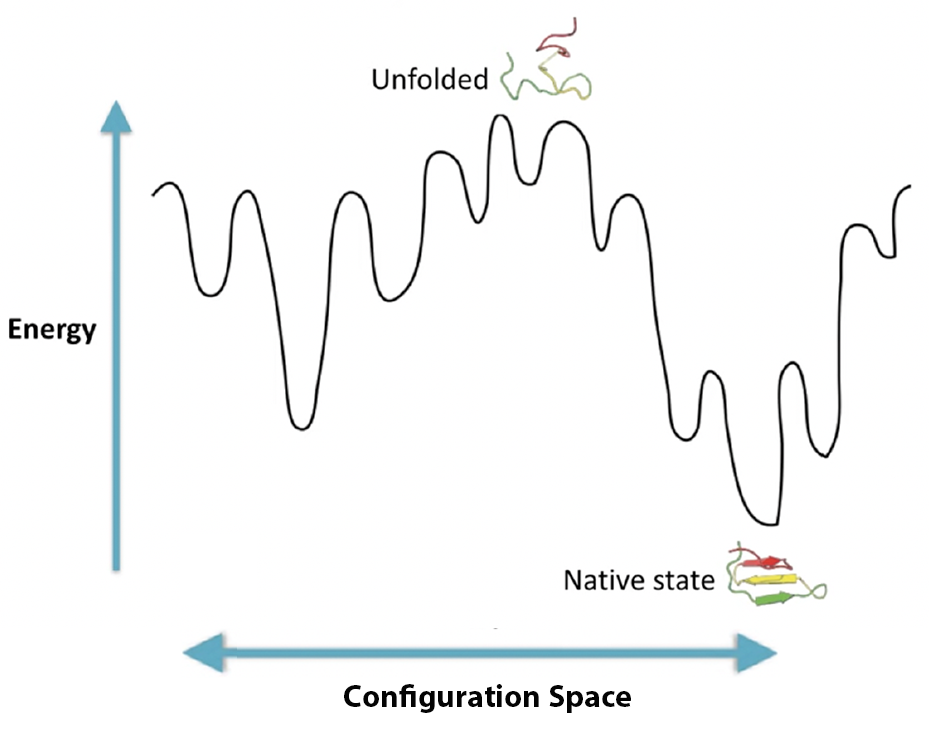
\includegraphics[width=\textwidth]{introduction/energy_landscape.png}
    \caption{Energy landscape.}
    \label{fig:landscape}
    \small
\end{figure}

To model all proteins coded by the human genome would require identifying the lowest energy structure for each of the fixed amino acids sequences for the 20 000 different proteins \cite{ponomarenko2016size}.  The protein folding research problem has been challenging for a number of reasons.  Firstly, a polypeptide chain can have a large number of different conformations; for each side chain in an amino acid in a protein there are a number of rotatable bonds with each amino acid having three different conformations leading to 3\textsuperscript{Nres} (Nres being the number of residues) possible conformations of every protein (Figure \ref{fig:angles_aa}).  Although the omega bond (peptide bond between the carbonyl carbon (C=O) of one amino acid and the nitrogen (N-H) of the adjacent amino acid in the peptide chain) is different as it is not really rotatable and results in the cis and trans forms \cite{craveur2013cis}.

\begin{figure}[th!]
    \centering
    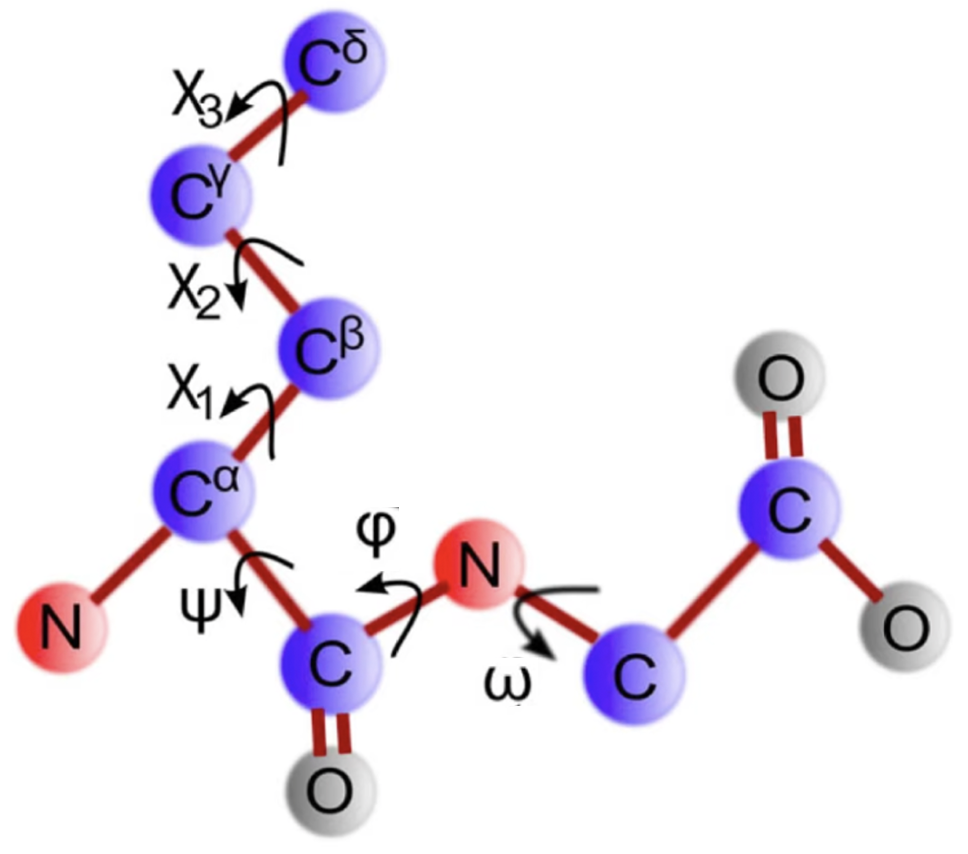
\includegraphics[width=\textwidth]{introduction/angles.png}
    \caption{Side-chain conformations.}
    \label{fig:angles_aa}
    \small
\end{figure}

Calculating the energy profile of a target protein was traditionally performed by searching through possible polypeptide chain conformations for a fixed sequence in an analogous way to how a protein naturally folds. For example Rosetta \cite{baker2001protein} simulates the actual process of folding to find the lowest energy structure rather than sampling all possible conformations.  The Rosetta folding takes place many times constructing 'decoys' to build an energy landscape to identify the lowest energy structure and therefore the most native-like structures. The folding algorithm utilises the fact that in some organisms separate genes encode interacting proteins, whereas in other organisms, their orthologues take the form of a single polypeptide chain \cite{hardin2002ab}. Therefore the structure of the protein can be viewed as a number of fragments that interact with specific kinetic and thermodynamic constraints.  During the ab initio folding process a Monte-Carlo search assembles these fragments with each assembly being scored based on a knowledge-based scoring function derived from the kinetic and thermodynamic constraints.  The model needs to capture detailed interactions between atoms therefore terms in the physics-based energy functions use mathematical means of modeling molecular interactions which need to favour:
\begin{itemize}
  \item close atomic packing (Lennard-Jones Potential \cite{jones1924determination});
  \item implicit solvation penalising buried polar atoms away from water;
  \item favour the formation of hydrogen bond interactions between polar atoms;
  \item model electrostatic interactions with the favourability of positive and negative charges to be close;
  \item model bending/torsional preferences of the polypeptide chain.
\end{itemize}
The calculation of an energy estimate or scoring function also takes the form of a knowledge-based function where statistical models define the properties of the native-like conformation. 

The method described greatly reduces the conformational search space.  However, additional strategies have also been employed to further reduce this search space.  Specifically for membrane proteins the Rosetta method was modified into a specific flavour, RosettaMembrane, where the energy function was modified to include terms that describe the interaction between target protein and the environment consisting of the anisotropic membrane. The membrane is modelled implicitly  with the energy terms including the scoring function that penalises non-helical torsion angles and non-spanning transmembrane helices within the membrane \cite{barth2007toward}.  



\section{Contact restraints used for Structure Prediction}
Contact-based modelling methods can address larger targets than conventional fragment-assembly-based ab initio methods \cite{Yang2020}. Contact-based modelling methods have been proven successful previously in modelling membrane proteins \cite{Hopf2012}.  Contact based restraints are determined by the introduction of co-variance data which supplies the additional restraints for the model building process by inferring residue-residue contacts.  The utilisation of contact predictions allows the generation of accurate ab initio models by guiding the folding process \cite{marks2011protein} .  This method led to the computational protein structure prediction for larger targets compared to what a solely fragment-assembly-based ab initio methods could construct \cite{Yang2020}. Additionally, contact-assisted ab initio modelling disposed of the need for membrane specialised folding methods like RosettaMembrane as these modelling methods have been proven successful previously in modelling membrane proteins \cite{Hopf2012,hopf2012three}.
Ab initio methods made significant strides when contact predictions were made available as modelling restraints \cite{Lee2016}. The definition of a contact is when the C$\beta$'s (C$\alpha$ in glycine) of two residues in three dimensional space are less than 8{\AA} apart.  For modelling purposes these binary contacts can be converted to distances, derived from experimental data, imposing further restraints on the modelling process \cite{braun2015combining}.   Prediction of residue-residue contacts relies on the fact that each pair of contacting residues co-varies during evolution. The process of co-variation occurs as the properties of the two residues complement each other in order to maintain structural integrity of that local region and, consequently, its original functionality (Figure \ref{fig:contacts}).  Therefore, if one residue from the pair is replaced, the other must also change to compensate the variation and hence preserve the original structure \cite{Lapedes}.  
\begin{figure}[th!]
    \centering
    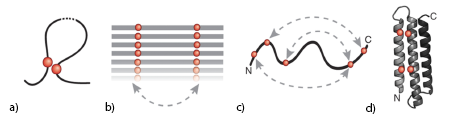
\includegraphics[width=\textwidth]{introduction/contacts.png}
    \caption{How residues separate in two-dimensions come together in three-dimensional space. }
    \label{fig:contacts}
    \small
    Interacting residues in a 3D structure compared to positions in a MSA displaying a co-evolving relationship. Adapted from \cite{Simkovic2017}.
    Co-evolutionary analysis used to infer contacts between amino acids in a protein by analysing the patterns of correlated mutations across a set of related protein sequences. a) The underlying assumption is that amino acids in close proximity within the protein structure tend to co-evolve due to their functional or structural interactions. b) Sequence Alignment: A multiple sequence alignment (MSA) is generated, which represents the amino acid sequences of related proteins. The MSA provides a basis for identifying patterns of conservation and variation across the protein family. c) based on the identified pairs of co-evolving positions, contact predictions are made, suggesting that these positions are likely in physical proximity within the protein structure. d) The inferred contacts can be visualised as a contact map or used to guide the modeling of the protein's three-dimensional structure.
\end{figure}

Initially contact prediction accuracy was limited due to transitive correlations where indirect covariation leads to a false positive contact generating noise in the prediction.  However, algorithms were developed where the link between two residues can be then reliably be detected in multiple sequence alignments. Methods included using a maximum entropy approach like direct coupling analysis (DCA) \cite{Morcos2011} or building a precision matrix (inverse co-variance matrix) like in contact prediction software PSICOV \cite{jones2012psicov}.  Early success with contact-assisted ab initio modelling of membrane proteins was made with EVfold and made use of the DCA approach in conjuction with Crystallography and NMR System (CNS) \cite{brunger1998crystallography}.  The use of contacts in this case led to substantial improvements in model accuracy for membrane proteins up to 360 residues in length and achieving RMSDs below 5{\AA} \cite{Hopf2012}.
Additionally,  machine learning algorithms were developed to predict contacts \cite{Wu2020} which was first observed in CONSIP2 \cite{kosciolek2016accurate} where evolutionary conservation was coupled with a traditional neural network with a sliding window approach. Later more advanced methods like RaptorX \cite{wang2018analysis} utilised a deep learning convoluted neural network (CNN).  CNNs are specifically designed to automatically extract hierarchical representations of input data by utilising convolutional layers, pooling layers, and fully connected layers \cite{albawi2017understanding}.  The latest methods such as TripletRes \cite{li2021deducing} exploit deep residual neural networks. Deep residual neural networks (ResNets) are a type of deep learning architecture that address the challenges of training very deep neural networks \cite{li2016demystifying}. Traditional deep neural networks suffer from the problem of vanishing gradients (where gradients are the rate of change of a function), where the gradients become very small as they propagate through many layers, leading to difficulties in training. ResNets alleviate this problem by skipping one or more layers, allowing the gradients to flow directly to the earlier layers during the training process \cite{li2016demystifying}. 

The predicted contacts can also be used for a range of analyses such as the identification of domain boundaries by analysing contact density profiles \cite{Rigden2002,Simkovic2017} and as a quality measure for ab initio models \cite{DeOliveira2016}.  Contacts can also be plotted into a two-dimensional contact map \cite{Simkovic2017} and be supplemented with other data, such as secondary structure prediction, for annotation \cite{sanchez2021conplot}.

Recent advances in contact predictions have meant more information can be extracted from MSAs allowing the prediction of residue distances rather than binary contacts.  The resultant distogram reveals more specific information in regard to predicted distances between residues in a target protein (Figure \ref{fig:distogram}). The prediction of inter-residue distances has dramatically improved the accuracy of ab initio modelling by imposing more restraints for the folding process \cite{du2021trrosetta}.  Initial attempts to go beyond binary contact prediction and predict residue distances was difficult. Methods were developed that attempted the use of regression to infer residue distances as they are real value features and therefore intuitive.  Advances were made in distance predictions when the problem was tackled as a classification problem and rather than inferring distances in {\AA} a set of bins for discrete distance values works much better with accuracy on par with contact predictions \cite{Greener2019}.

\begin{figure}[htb]
\begin{subfigure}{0.5\textwidth}
  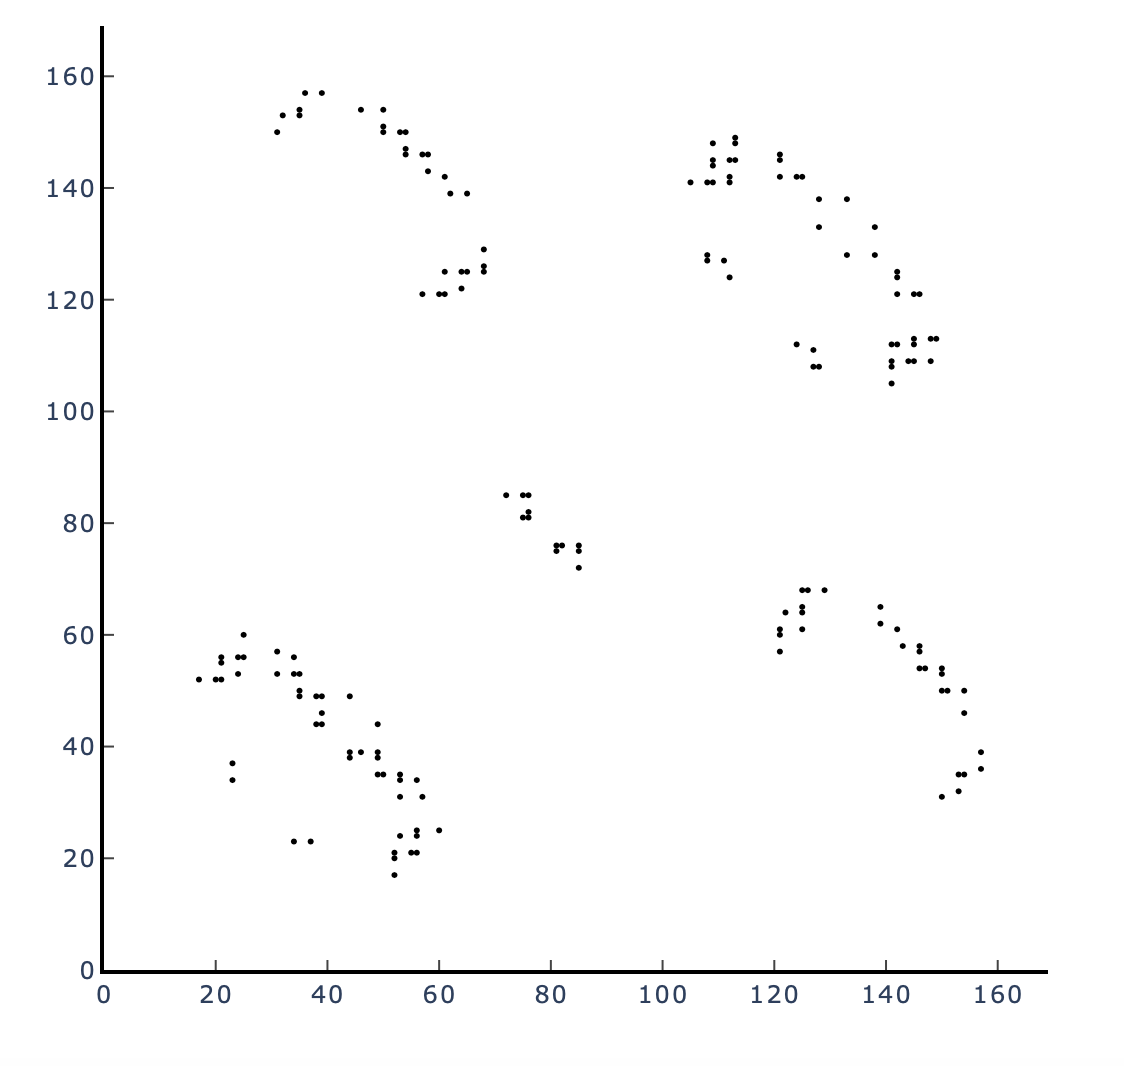
\includegraphics[width=\linewidth]{introduction/contact_map.png}
  \caption{Example contact map}
  \label{fig:4yms}
\end{subfigure}\hfil % <-- added
\begin{subfigure}{0.55\textwidth}
  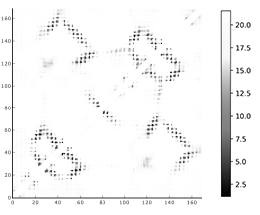
\includegraphics[width=\linewidth]{introduction/distogram.png}
  \caption{Example distogram}
  \label{fig:5do7}
\end{subfigure}\hfil % <-- added
\caption{Contact map and distogram comparison}
\small{Contacts are coloured black in the contact map; in a distogram each inter-residue pain is coloured based on a spectrum relating to the predicted distance of each specific pair of residues (in this case white to black)}
\label{fig:distogram}
\end{figure}


\section{Use of Deep Learning Algorithms for Membrane Protein Structure Prediction}
Classical protein structure prediction aimed, given a sequence, to search for the three-dimensional fold that dominates the partition function (statistical likelihood) and has the lowest free energy, making it the state most observed in nature.  The prediction of protein structure therefore possessed the twin core challenges of conformation search, ruled by Levanthal's paradox (identifying a protein's native fold by searching randomly takes an enormous amount of time yet a protein folds in seconds), and the scoring challenge, adhering to Anfinsen's dogma (the three-dimensional fold is determined by the amino acid sequence).   The well established fragment assembly ab initio approaches described in the previous section build protein models by utilising a function that models the postulates and theory derived from experimental data.  The fragment assembly methods, however, consume a high amount of computing resources and have the drawback of requiring native-like fragments being available. These methods, even with the inclusion of contact derived restraints, were only able to output reliable models for a tiny fraction of the protein universe and were especially poor for those with contact dense topologies \cite{leman2020macromolecular}.  Converting the contact information into predicted distance geometry constraints, similar to what is performed in NMR structure determination, is computationally cheaper and has been shown to produce models that are closer to their native state \cite{havel1991evaluation}.  Recently, methods such as AlphaFold, AlphaFold2 and RosettaFold have developed machine learning algorithms that predict distances which are used to generate accurate models by generating minimised free energy surface along the molecular coordinates (family-specific potentials of mean force).  The machine learning methods, or deep learning if the number of neural network layers are greater than six, construct a function to build a model by extracting features from an input data set and linking these to labels of the output data set.  Training the program involves it going back and forth in an automated fashion, taking the outputs and comparing to the inputs until a link between output and input is established.  This is similar to the classical approach where experimental data was used to construct functions that make predictions, and if the prediction were not accurate more data is gathered to refine the rules of the function; a very laborious and time consuming process.  With machine learning the function is built much more quickly with the experimental data not being used explicitly but  inferred through the learning that has taken place by linking the input features of models in the PDB (sequence) to the labels of the output structures (for example inter residue distances, main chain hydrogen bond network and torsion angles)(Figure \ref{fig:model_building}).
\begin{figure}[th!]
    \centering
    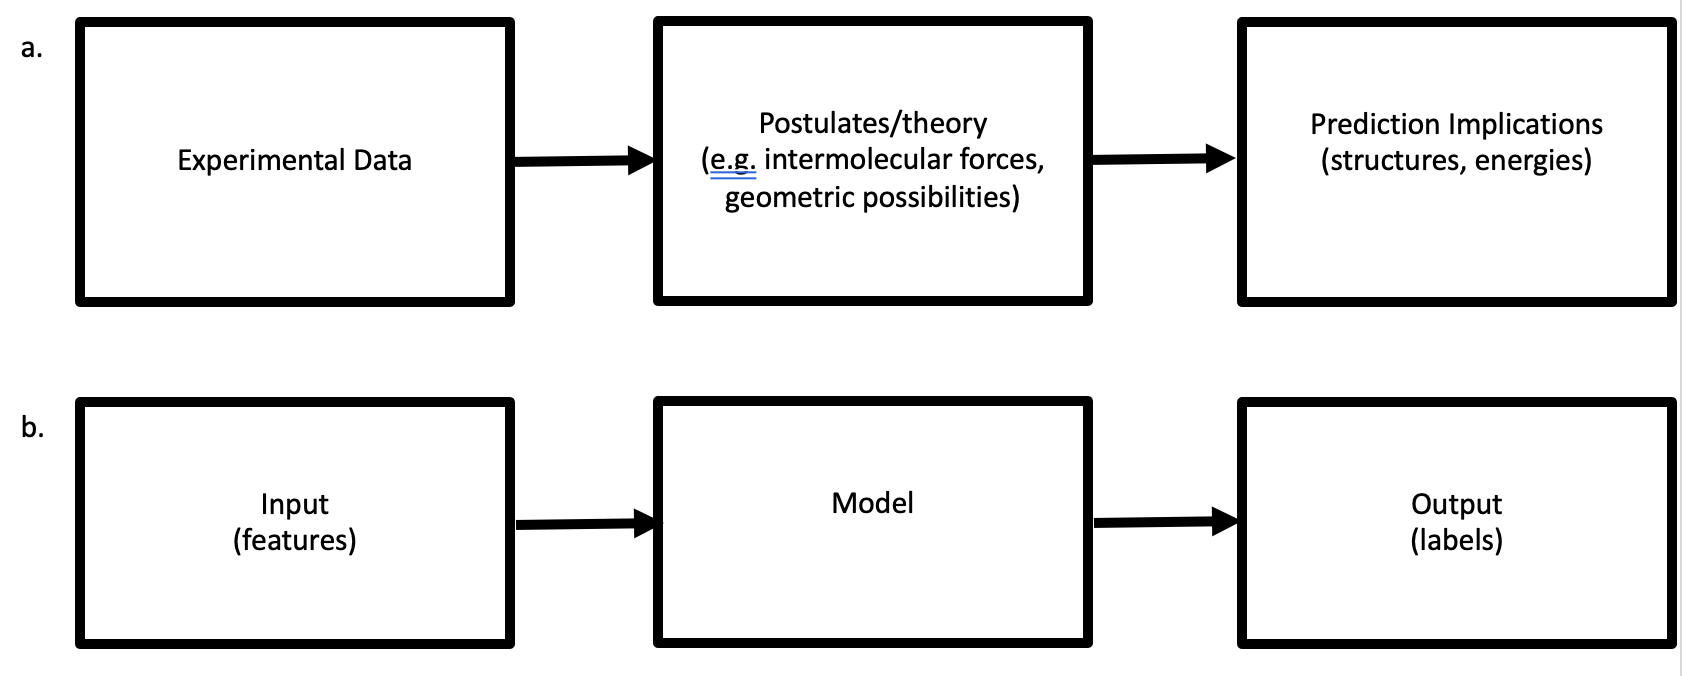
\includegraphics[width=\textwidth]{introduction/model_building.png}
    \caption{Comparison of the model function building between classical (a) and machine learning (b) methods}
    \label{fig:model_building}
    \small
\end{figure}

The deep learning methods such as AlphaFold \cite{Jumper2021}, DMPfold \cite{Greener2019} and trRosetta \cite{yan2021accurate} build predicted protein structures by predicting inter residue distances, main chain hydrogen bond network and torsion angles.  Benchmarking these methods has demonstrated that they work just as well for membrane proteins as they do for soluble proteins \cite{Greener2019,hegedHus2021alphafold2}.  DMPfold was shown to be able to model 26 of the 28 transmembrane proteins with a TM-score of at least 0.5 to the native structure and a mean TM-score of 0.74 \cite{Greener2019}.  The accuracy of AlphaFold2 transmembrane protein modeling has been tested by exploring the construction of structures from the ABC protein superfamily. For these transmembrane proteins AlphaFold2 performed exceedingly well when testing template-free structure prediction as well as attempting a new ABC fold, dimer modeling, and stability in molecular dynamics simulations \cite{hegedHus2021alphafold2}.  

\section{Exploitation of Advanced Methods}
This thesis details the utilisation of the methods described to build models of three intracellular organelle residing integral membrane proteins.  Unusual structural features are predicted during the investigation and subsequently methods for screening membrane proteins possessing these features were implemented. The work carried out during this PhD intersects with the unexpected acceleration in the field of protein structure prediction initiated in CASP13 with the release of AlphaFold \cite{Jumper2021}. The release of the accurate deep learning protein structural prediction methods half way through the PhD gave the opportunity to modify research plans in order to take advantage of these fast and accurate methods.  For example, in Chapter 3, a topology was mapped for the protein Tmem41b using contact map analysis; with the release of DMPfold, an accurate three dimensional model could be constructed which displayed the re-entrant loops that fragment assembly methods could not build.  Furthermore, the release of the AlphaFold database \cite{david2022alphafold} enabled a library of trRosetta models to be enriched with the more accurate AlphaFold equivalents; this enabled us to search for specific structural motifs within a library of high quality models that had no experimental structures (Chapter 5).  The field of protein structure is currently moving at a very fast pace and I feel privileged to have been in this field, as a researcher utilising these bioinformatic methods as well as my role as a CASP assessor in CASP14, at this very important juncture.   



\chapter{General Experimental Methods}
\section{Choice of Methods}
Initial methods utilised contact assisted (converted to distance restraints) fragment assembly modelling tools, both general and membrane specific protocols, to perform membrane protein structure prediction; Rosetta ab initio and RosettaMembrane.  As the PhD progressed, deep learning methods became available and these were exploited to generate more accurate predicted structures; first DMPfold then trRosetta followed by AlphaFold2 (prior to the release of AlphaFold2 AlphaFold models from the AlphaFold database were used).

Accurate contact predictions were required to guide the fragment assembly modelling process and distance predictions were required for modelling using the deep learning methods.  In order to obtain as accurate contact and distance predictions as possible, multiple sequence alignments were required not only to be as deep as possible but also sequences need to be as diverse as possible with both the magnitude of depth and diversity being related to the length of the query protein sequence \cite{ovchinnikov2015large}. The function relating these three variable is known as the Number of Effective Sequences (Neff) and is the ratio of number of sequence clusters at an 80\% sequence identity clustering threshold to the square root of the protein length \cite{ovchinnikov2015large}.  Neff has been shown to positively correlate with contact prediction and model accuracy \cite{Ovchinnikov2017}.  Attempts were made to increase Neff values of MSAs by generating them using metagenomic sequence databases. When implemented, the Neff does indeed increase, however, in some cases the contact prediction derived from a metagenomic database contained less detail compared to solely using Uniprot i.e signals for some contacts were completely lost (Figure \ref{fig:cmap_degrade}). 

\begin{figure}[th!]
    \centering
    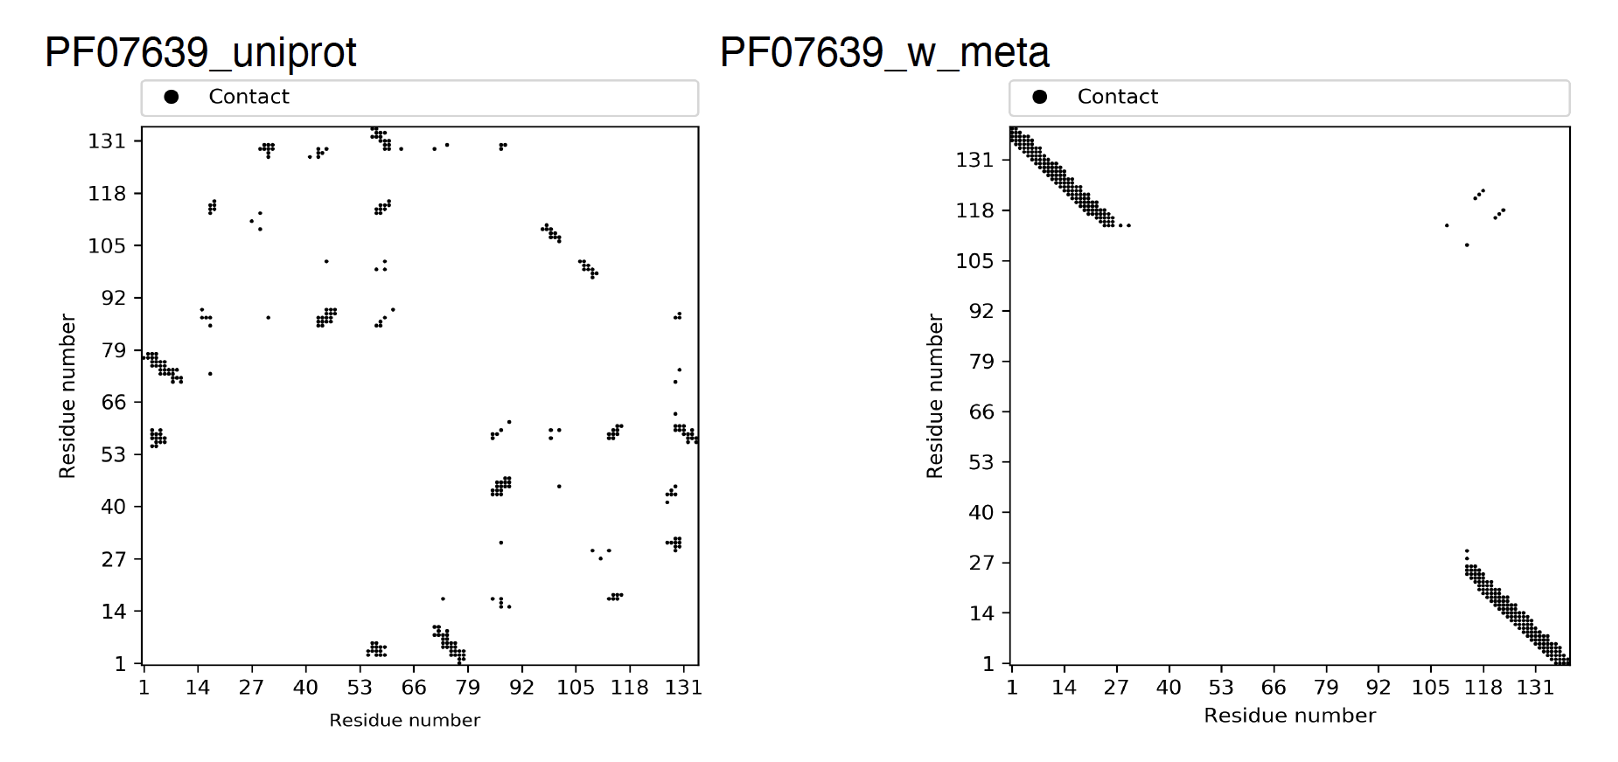
\includegraphics[width=\textwidth]{Experimental Methods/Screenshot 2022-08-02 at 12.14.54.png}
    \caption{Comparison of contact maps constructed with (right) and without (left) metagenomic sequence data.}
    \label{fig:cmap_degrade}
    \small
    Contact were derived using DeepMetaPsicov with the representative sequence for the Pfam domain PF07639.
\end{figure}

Additionally, the use of a metagenomic database made it difficult to maintain annotations as they lack reliable source organism information therefore making the use of phylogeny to link structure to function more difficult.  Therefore any use of metagenomics was considered carefully before implementation.

Results chapters 3 and 4 describe the structure-function investigation into two different autophagy proteins.  Chapter 5 describes the search for specific structural motifs from a number of structural databases.  Methods utilised that were common to more than one chapter are described here with chapter specific methods detailed in the relevant chapter.

Local installations and runs were made on a Ubuntu 18.04.6 workstation  AMD Ryzen Threadripper 2990WX 32 Core CPU (3.0GHz, 80MB CACHE). 64GB Corsair VENGEANCE DDR4 2933MHz ~ (8 x 8GB) was installed.  GPU acceleration was not used for the earlier model building and the graphic card installed was a PNY QUADRO P620 - 2GB GDDR5, 512 CUDA Cores - 4 x mDP.  The required databases were located over two 4TB SEAGATE BARRACUDA SATA-III 3.5" HDD, 6GB/s, 5400RPM, 256MB CACHE.

Model building for the Oca2 protein utilised a local instalation of ColabFold and exploited GPU acceleration via the ASUS TUF GeForce RTX 3080 OC LHR 12GB GDDR6X Ray-Tracing Graphics Card, 8960 Core, 1815MHz Boost.

\section{Software}

\subsection{Pfam Database Screening}
In order to screen the Pfam database with query sequences the HMM-HMM comparison tool, HHpred \cite{El-Gebali2019} (Homology detection and structure prediction by HMM-HMM comparison) was used. HHpred utilises Hidden Markov Models (HMMs) and compares a query protein sequence against a database of profile Hidden Markov Models. HHpred generates a profile Hidden Markov Model from the query sequence. This profile HMM captures the statistical properties and patterns of the query sequence.  HHpred searches a database of profile HMMs, such as the Pfam.  It compares the profile HMM of the query sequence against the profile HMMs in the database.  HHpred performs a sequence-sequence alignment between the query sequence and the database sequences that show significant similarity based on the profile HMM comparison. HHpred then calculates consensus alignments and generates alignment scores, such as the E-value (expectation value - is a statistical measure that estimates the number of false positives expected to be found by chance in a database search; the lower the more significant) and probability score, to assess the significance of the matches. These scores indicate the likelihood of homology and similarity between the query sequence and the matched protein structures. Typical threshold values for probability in HHpred range from 90\% to 95\%, meaning that only matches with a probability above the specified threshold are considered significant.
The threshold for the E-value is typically set to a small value, such as 0.01 or 0.05, implying that only matches with E-values below the threshold are considered significant.

Sequence based searches against the PDB and Pfam-A\_v32.0  databases used the locally installed HHPred v3.0 \cite{Zimmermann2018} with default parameters and eight iterations for MSA generation in the HHblits \cite{Remmert2012} stage;

\begin{lstlisting}[style=linux-terminal]
hhblits -p 20 -Z 10000 -loc -z 1 -b 1 -B 10000 -ssm 2 -sc 1 -seq 1 -dbstrlen 10000 -norealign -maxres 32000 -contxt /path/to/context\_data.crf
\end{lstlisting}

\subsection{Contact map predictions (Metagenomic)}
The MSAs were generated using Jackhmmer v3.3 \cite{Johnson2010}, default parameters with five iterations against a custom metagenomic database. The metagenomic database was a concatenation of: EupathDB \cite{Aurrecoechea2017}, Uniref100 \cite{Apweiler2004}, the Marine Eukaryotic Reference Catalogue (MERC) \cite{Steinegger2018}, the Soil Reference Catalogue (SRC) \cite{Steinegger2018}, MGnify \cite{Mitchell2019}. Local installations of DeepMetapsicov v1.0  \cite{Kandathil2019} and ResPre \cite{Li} were used to generate contact predictions with ConKit v0.12 \cite{conkit2017} utilised to visualise the contact maps. ConPlot was used to overlay additional prediction data \cite{sanchez2021conplot}.

\subsection{Model Building}
\subsubsection{Model building: Rosetta Ab initio}
Rosetta version 3.10 suite \cite{raman2009structure} was used for the initial Roestta model building. Rosetta uses the distribution of local structures in related sequences of solved structures to approximate structures of fragments in the query protein. These short structures are then assembled via a Monte Carlo search with a scoring function based on conformational statistics; Rosetta energy function.  The Rosetta energy function is derived from statistical analysis of known protein structures and incorporates various terms to estimate the energy associated with different aspects of protein conformation, such as bond lengths, angles, and non-bonded interactions \cite{baker2001protein}. 

The Rosetta flag file contains the paths for the fasta sequence, the PSIPRED \cite{McGuffin2000} secondary structure prediction, 3mer/9mer fragments, and the restraint files.

Fragments for the Rosseta Ab initio model building were generated using the local installation of Rosetta Fragment Picker:

\begin{lstlisting}[style=linux-terminal]
/path/to/fragment_picker.linuxgccrelease @best-frags.flags -in::file::vall /path/to/vall.apr24.2008.extended.gz
\end{lstlisting}

Restraint files were generated using python scripts available with the Rosetta distribution; 'create\_evfold\_contact\_map.py' converts contact data (in EVfold \cite{braun2015combining}) to a compatible format that is acceptable c to 'extract\_top\_cm\_restraints.py' \cite{braun2015combining} to create a '.cst' file.  The '.cst' file lists predicted distances generated from the contact data that is used by Rosetta to read and implement the restraints.

\begin{lstlisting}[style=linux-terminal]
/path/to/AbinitioRelax.linuxgccrelease @/flags_tmem41b
\end{lstlisting}


\subsubsection{Model building: RosettaMembrane}
The RosettaMembrane protocol \cite{yarov2006multipass} uses, in addition to the fasta sequence, PSIPRED secondary structure prediction \cite{McGuffin2000}, 3er/9er fragments, and the restraint files, a membrane topology prediction file.  An OCTOPUS \cite{Viklund2008} prediction file is processed using the 'octopus2span.pl' Perl script.  The output file is then further processed into a format acceptable to RosettaMembrane using the 'run\_lips.pl' script;

\begin{lstlisting}[style=linux-terminal]
/path/to/run_lips.pl ../tmem41b.fasta ./tmem41b.span /path/to/blastpgp /db_blast/nr /path/to/alignblast.pl
\end{lstlisting}


The script did have to be modified due to it attempting to run a CGI script (lips.txt) that was no longer available remotely; the url is not run as a CGI (Common Gateway Interface) script, it was just where the script could be downloaded from. A CGI  script allows interaction between a web server and other software applications, enabling dynamic content generation and processing of user requests. CGI scripts are commonly used to perform tasks such as processing form data and interacting with databases. When a user submits a request to a web server, the server can execute a CGI script to process the request and generate a response. The CGI script can receive input parameters from the user's request, perform necessary computations or operations, and generate an output. In this case as the CGI script was no longer available the script was run locally by downloading (http://tanto.bioe.uic.edu/lips/lips.txt), made executable and the run\_lips.pl was made to point at the local script rather than the url by modifying line 132 in order to execute the local version of the script;

\begin{lstlisting}[style=linux-terminal]
$data=`curl -s $url -d sequence='$sequences' -d num=$first_num`;
\end{lstlisting}
to \\

\begin{lstlisting}[style=linux-terminal]
$data=`/rosetta/lips.txt -d sequence='$sequences' -d num=$first_num`;
\end{lstlisting}

The RosettaMembrane is then executed with the appropriate flag file;

\begin{lstlisting}[style=linux-terminal]
/path/to/membrane_abinitio2.linuxgccrelease @ ./flags_membrane.txt
\end{lstlisting}

\subsubsection{Clustering of Rosetta Decoys}
SPICKER \cite{Zhang2004} (SPatial Clustering with Kernels) is a protein structure clustering algorithm used to group similar protein structures based on their three-dimensional coordinates. SPICKER takes a set of protein structures as input, typically represented by their Cartesian coordinates (x, y, z) of atoms. SPICKER then calculates the pairwise root-mean-square deviation (RMSD) distances between all pairs of structures. RMSD measures the structural similarity between two protein structures by quantifying the average distance between corresponding atoms after superimposition. SPICKER employs a kernel density estimation technique to estimate the density of structures in the multi-dimensional RMSD space. It constructs a density function by assigning each structure a probability density value based on its RMSD distance to other structures.v The density-based clustering algorithm DBSCAN (Density-Based Spatial Clustering of Applications with Noise) is applied to identify clusters in the estimated density function. DBSCAN groups structures that have high density and are closely located in the RMSD space. Structures that are not in any cluster are considered as noise.  SPICKER selects the most representative structure from each cluster based on the average RMSD distance to other structures in the same cluster. This representative structure is often referred to as a "centroid" or "medoid" and is used to represent the cluster.

SPICKER \cite{Zhang2004} was used to cluster the output models from Rosetta.  SPICKER was executed within the ccp4 suite which auto generates the required input files.

\begin{lstlisting}[style=linux-terminal]
ccp4-python /path/to/spicker.py -e /path/to/spicker -m ./models/ -t 50 
\end{lstlisting}



\subsubsection{Model building: trRosetta}
Ab initio models were built using the trRosetta \cite{Yang2020} local installation with default settings utilising an MSA from HHblits in the '.a3m' format. Transform-restrained Rosetta (trRosetta) is a Rosetta protocol that utilises predicted distances and orientations as restraints that are derived from a deep residual-convolutional network.  The network takes an MSA as input and the outputs are used as energy minimisation restraints in the Rosetta model building.  This differs from Rosetta contact assisted ab initio model building as in addition to the C$\beta$–C$\beta$ distances the orientations (defined by six parameters) are predicted which accurately describe the relative positions of the backbone of two residues.

The predicted distances and side-chain orientations were generated using:
\begin{lstlisting}[style=linux-terminal]
python ./predict.py -m ./model2019 example/T1001.a3m example/T1001.npz
\end{lstlisting}
Models are constructed using trRosetta by:
\begin{lstlisting}[style=linux-terminal]
python trRosetta.py T1008.npz T1008.fasta model.pdb
\end{lstlisting}

\subsubsection{Model building: DMPfold}
DMPfold \cite{Greener2019} utilises deep-learning to predict inter-residue distances, main chain hydrogen bond network and torsion angles.  These are then used in the model building process. The Ab initio models were built using a DMPfold local installation with default settings utilising an MSA built by Jackhmmer.  The alignments in '.aln' format is then used by a DMPfold script to generate distance restraints: 
\begin{lstlisting}[style=linux-terminal]
csh aln2maps.csh example/PF10963.aln
\end{lstlisting}
The restraints were then used to build the models:
\begin{lstlisting}[style=linux-terminal]
/path/to/DMPfold/run_dmpfold.sh /w9dy28.fasta ../output.21c ../output.map ./w9_1_84_models
\end{lstlisting}

\subsubsection{Homology Modelling}
Homology modeling, also known as comparative modeling, is a computational method used to predict the three-dimensional structure of a protein based on its sequence similarity to one or more known protein structures. It relies on the principle that proteins with high sequence similarity share similar structures and functions. A target protein, is selected for which the experimental structure is unknown but a related template structure with known three-dimensional coordinates exists. Suitable template structures are identified by searching sequence databases using algorithms such as HHpred. Templates with high sequence similarity to the target are preferred, ideally with sequence identity above a certain threshold (e.g., 30-40\%). The target protein sequence is aligned with the template sequence to identify corresponding positions and regions. Using the sequence alignment as a guide, the three-dimensional coordinates of the target protein are constructed by copying the coordinates from the template structure. The quality and reliability of the homology model are assessed using various validation criteria and scoring functions. This study employed predicted contact satisfaction scores (see below). MODELLER \cite{eswar2006comparative} is a software package widely used for homology modeling and comparative protein structure prediction and was used for the study of Atg9 (Chapter 4). 

\subsection{Transmembrane Region Prediction}
Unless otherwise stated the transmembrane helical topology predictions were obtained from the Topcons server \cite{Tsirigos2015}. TopCons combines multiple sources of information, including predicted transmembrane helices, signal peptides, and homologous proteins, to make accurate predictions.  Based on this combined information from signal peptide prediction, transmembrane helix prediction, and homology-based prediction, TopCons generates a consensus prediction for the presence and location of transmembrane regions in the protein sequence.

When confidence scores were required for individual transmembrane region predictions TMHMM (TransMembrane Hidden Markov Model) was employed. TMHMM employs a Hidden Markov Model (HMM) approach.  TMHMM is trained using a dataset of known transmembrane proteins with experimentally verified transmembrane helices. The HMM is trained to recognize the statistical patterns and properties associated with transmembrane regions.

Other transmembrane prediction software was utilised for comparison purposes:
\begin{enumerate}
\item Octopus \cite{viklund2008octopus};
\item Spoctopus \cite{teixeira2017membrane}; 
\item Philius \cite{reynolds2008transmembrane} ;
\item Polyphobius \cite{jones2007improving} ;
\item SCAMPI \cite{reeb2015evaluation};
\end{enumerate}

\subsection{Secondary Structure Prediction}
Secondary structure predictions were made employing a local installation of PSIPRED v4.0 \cite{McGuffin2000}. (Protein Structure Prediction Server). PSIPRED employs a  neural network to make its predictions. PSIPRED Generates a position-specific scoring matrix (PSSM). A PSSM is a matrix that encodes the sequence profile, which represents the frequency and propensity of each amino acid at each position in the sequence. The PSSM is generated by performing a sequence database search using tools like PSI-BLAST \cite{altschul1998iterated}. The final output of PSIPRED is a prediction of the secondary structure for each residue in the protein sequence. This prediction is usually represented as a sequence of letters corresponding to the predicted secondary structure states (H for alpha helix, E for beta strand, and C for coil).

\subsection{Conservation Mapping}
Conservation was mapped on to the models using the ConSurf server \cite{Ashkenazy2016}. 

To visualise the conservation as a spectrum using Consurfs conventional spectrum the Consurf processed PDB file (with updated with ConSurf colours - PDB\_FILE) and the python script, consurf\_new.py, was downloaded from the server; PyMol was then initialised and the processed PDB file was loaded with the subsequent run of the consurf\_new.py script ('run consurf\_new.py' in PyMol terminal);


\subsection{Visualisation of Models}
Visualisation of models was achieved using PyMOL v2.3.0 \cite{DeLano2002}.

Membrane planes were visualised by:

\begin{enumerate}
\item Downloading membrane\_planes.py \cite{baugh2011real} from RosettaCommons and place in the same directory as the PyMol executable;
\item Downloading visualise\_membranes.pml from RosettaCommons the attached .pml \cite{baugh2011real} file;
\item Download the translated version of the pdb file from PDBTM or generate the translated version from the OPM server; 
\item Initialise pymol with a command like the following;  
\begin{lstlisting}[style=linux-terminal]
/path/to/PyMOL ./3org.pdb ./visualize_membrane.pml  (/path/to/pymol/executable/ /path/to/translated/pdb/file/ /path/to/pml/file)
\end{lstlisting}

\end{enumerate}

\subsection{Structural Alignments}
Structural alignment methods aim to compare and align protein structures to identify similarities, infer evolutionary relationships, and gain insights into their functional and structural properties. There are many methods for assessing similarity \cite{Holm2016,orengo199636,falicov1996surface,krissinel2004secondary} and commonly rely on comparing the sizes of shared substructures, such as the length of alignment, where longer alignments are considered more favorable. Additionally, a distance measure like RMSD (Root Mean Square Deviation) is commonly used to evaluate the difference between these substructures, with lower values indicating greater similarity.  RMSD  quantifies the average distance between corresponding atoms in the two sets of coordinates. It is calculated by aligning the structures and measuring the displacement of each atom.  The distance between each pair of corresponding atoms in the superposed structures is calculated. The deviation or displacement of each atom is obtained by subtracting the position of the corresponding atom in one structure from the position of the corresponding atom in the other structure. The deviations are squared, and the squared deviations are summed across all atoms in the structure. The summed squared deviations are divided by the number of atoms, and the square root of the result is taken to obtain the RMSD value \cite{yusuf2008alternative}.  

\[ \text{RMSD} = \sqrt{\frac{\sum\limits_{i=1}^{n}(x_i - y_i)^2}{n}} \]

\begin{itemize}
\item  \(N\) is the total number of atoms.
\item  \(\mathbf{X}_i\) and \(\mathbf{Y}_i\) denote the coordinates of the corresponding atoms in the two compared structures.
\item  The summation \(\sum_{i=1}^{N}\) iterates over all the atoms.
\item  \((\mathbf{X}_i - \mathbf{Y}_i)^2\) calculates the squared differences between the corresponding atom coordinates.
\end{itemize}
RMSD is expressed in units of length. A lower RMSD value indicates a closer match between the structures, while a higher RMSD value suggests greater differences or structural variation.

Local installation of Dali v4.0 \cite{Holm2016} was used to structurally align the output models and to query against the PDBTM \cite{Kozma2012}.  Dali has high sensitivity in detecting structural similarities identifying remote homologues and recognise similarities even when sequence similarity is low.  Dali is capable of handling both small and large protein structures and can align multiple structures simultaneously, enabling the detection of structural relationships among a set of proteins.  Dali provides Z-scores that assess the significance of the structural similarity. This statistical measure helps evaluate the reliability of the alignments and distinguish true similarities from random matches. Z-scores provide a measure of how well the observed similarity score (DALI Z-score) compares to the scores obtained from random structure alignments.  First Dali generates random structural alignments by shuffling and superimposing the secondary structure elements of the two proteins being compared. This generates a distribution of similarity scores for random alignments.  The similarity score used in Dali is the Z-score-like score, which is based on the root mean square deviation (RMSD) between aligned residues, the number of aligned residues, and the length of the proteins. The Z-score is then calculated by comparing the similarity score of the observed alignment with the distribution of scores obtained from the random alignments. It represents the number of standard deviations the observed score is away from the mean of the random distribution. A higher Z-score indicates a higher level of significance for the structural similarity.


\subsection{Precision}
Precision score evaluation of models in relation to the predicted contacts at various contact cutoff values were calculated and plotted using ConKit. A 70\% precision cut off  for the top L contacts is suggestive of good quality models \cite{DeOliveira2016}.
%where L = sequence length (rounded down to the nearest whole number of contacts)


\subsection{Other prediction data}
ConKit was also used to predict and visualise potential structural domain boundaries \cite{Rigden2002}\cite{Simkovic2017}. Residue analysis of putative amphipathic regions were performed using HELIQUEST \cite{Gautier2008} to determine the presence, direction and magnitude of any hydrophobic moment. 

\chapter{\emph{In silico prediction of structure and function for a large family of transmembrane proteins that includes human Tmem41b}}

\section{Introduction}
Recent strides in computational structural biology have opened up an opportunity to understand previously uncharacterised proteins.  The under-representation of transmembrane proteins in the Protein Data Bank highlights the need to apply new and advanced bioinformatics methods to shed light on their structure and function. 

Membrane proteins can be grouped according to their interaction with various cell membranes: integral membrane proteins (IMPs) are permanently anchored whereas peripheral membrane proteins transiently adhere to cell membranes. IMPs that span the membrane are known as transmembrane proteins (TMEMs) as opposed to integral monotopic membrane proteins that adhere to one side of the membrane \cite{Fowler2006}. Membrane proteins also include various lipid-modified proteins \cite{Resh2016}.

Autophagy-related proteins (Atg) are responsible for the formation of autophagosomes that traffic unwanted intracellular components to the lysosomes for degradation.  Atg9 (Chapter 4) is the only established transmembrane Atg \cite{guardia2020structure}, however, there is a growing body of evidence that two proteins belonging to the Pfam PF09335 family may also be transmembrane Atgs; Tmem41b and Vmp1 \cite{Morita2019}. 

In this chapter, the Pfam PF09335 family is linked to the PF06695 family and a conveniently small archaeal sequence was identified. Subsequently, utilising state of the art methods, structural predictions for not only the archaeal sequence but also for two prominent members of the Pfam family PF09335 (Tmem41b and YqjA) were made. In order to carry out these predictions, data derived from sequence, evolutionary covariance and ab initio modelling was exploited. The result of the modelling indicated that both PF09335 homologues (DedA proteins) and PF06995 homologues contain re-entrant loops (stretches of protein that enter the bilayer but exit on the same side of the membrane).  Additionally, the predictions also anticipate that the re-entrant loops form part of a pseudo-inverted repeat topology. The predicted presence of both of these structural features strongly suggests that DedA proteins are secondary active transporters for an uncharacterised substrate.


\section{DedA Proteins}
The family Tmem41 has two human representatives, namely Tmem41a and Tmem41b; both share the PF09335 ('SNARE{\_}ASSOC'/ ‘VTT‘/’Tvp38’/’DedA’) Pfam \cite{El-Gebali2019} domain. The profile of Tmem41b has recently risen due to experimental evidence pointing to its involvement in macroautophagy regulation (making it a possible Atg protein, i.e. an autophagy related protein) and lipid mobilisation \cite{Moretti2018}. Other studies identify Tmem41b to be involved in motor circuit function, with TMEM41B-knockout \emph{Drosophila melanogaster} showing neuromuscular junction defects and aberrant motor neuron development in SMN1 knockout zebrafish \cite{Lotti2012}. Also, it has been reported that in TMEM41B-knockout HeLa cells there is an inhibition of Zika virus replication \cite{Scaturro2018}. Tmem41b has also been identified as a host cell factor for SARS-CoV-2 \cite{Schneider2020}. Tmem41b is the only common host cell factor identified for flaviviruses and coronaviruses and is the only autophagy-related protein identified as a viral host factor \cite{Hoffmann2021}.\\
Additionally, Tmem41b has been shown to be essential for mouse embryonic development: homozygous knockout mice embryos suffer early termination of their development after 7–8 weeks \cite{VanAlstyne2018}. Tmem41b is a structurally uncharacterised 291-residue protein found in the endoplasmic reticulum (ER) localising at the mitochondria-associated ER membranes \cite{Moretti2018}. Disruption of the PF09335 domain by various residue substitutions \cite{Tabara2019} or its removal \cite{Moretti2018} results in inhibition of autophagosome formation and impaired lipid mobilisation in human embryonic kidney (HEK) cells.\\
Tmem41b homologues, hereafter referred to as DedA proteins \cite{Morita2019}, are present in all domains of life \cite{Keller2013}. The Pfam PF09335 domain was first identified in the \emph{Saccharomyces cerevisiae} protein Tvp38 \cite{Inadome2007}, and the authors concluded that Tvp38 associates with SNARE proteins (SNAP REceptor).  SNARE proteins are responsible for the fusion of vesicles with a target membrane.  Specifically, Tvp38 was shown to associate with t-SNARE sub-types in Tlg2-containing compartments, suggesting a role in membrane transport. Investigations into the bacterial and archaeal prevalence of these proteins showed that 90\% of bacterial species and 70\% of archaeal species encode proteins with the PF09335 domain \cite{Doerrler2013}. Bacterial and archaeal PF09335-containing proteins are collectively known as the DedA family \cite{Doerrler2013,nonet1987hist}. Detailed studies of the \emph{Escherichia coli} DedA proteins have indicated that there are eight E. \textit{coli} representatives of the DedA family (YqjA, YghB, YabI, YohD, DedA, YdjX, YdjZ, and YqaA) with overlapping functions \cite{Doerrler2013,Keller2013}, with YdjX and YdjZ being the most closely related to human Tmem41b in terms of sequence similarity \cite{Doerrler2013}. Phenotypically, DedA knock-out \emph{E. coli} cells display increased temperature sensitivity, cell division defects, activation envelope stress pathways, compromised proton motive force, sensitivity to alkaline pH and increased antibiotic susceptibility \cite{Doerrler2013}\cite{Keller2014}. As \emph{E. coli} expresses multiple DedA homologues, lethal effects are not observed as long as at least one DedA is expressed \cite{Keller2014}\cite{Thompkins2008}. \emph{Borrelia burgdorferi} contains only one DedA protein in its genome and knockout cells display the same phenotype as the \emph{E. coli} knockout strains.  The \emph{B. burgdorferi} homologue is indeed essential \cite{Feng2010}. Interestingly, \emph{E. coli} knockout cells can be rescued with the B. burgdorferi homologue that shows only 19\% sequence identity with YqjA. The functions of DedA have also been studied in the pathogen \emph{Burkholderia thailandensis} where one family member was found to be required for resistance to polymyxin \cite{Panta2019}.

\section{Specific Methods}
This PhD coincided with a rapid development in the field of ab initio structure prediction.  The most advanced methods at the time were always utilised and as new methods and model databases were released these were employed to gather additional structural information as well as to validate previous modelling attempts. 

\subsection{Model building: trRosetta}
In order to test whether the modelling software could accurately capture the re-entrant loop-helix structural motif, a model representing the crystal structure of 6cb2 was constructed using both trRosetta and DMPfold \cite{Greener2019}. The crystal of 6cb2 is comparable in terms of size (293 residues) and has the common structural features (inverted repeat with two re-entrant/TMhelix structures) to the Tmem41b and its homologous proteins.  The output structure was structurally aligned against the crystal structure using DALI (server) and a gave Z-score of 35 for the trRosetta with 27.5 for the DMPfold equivalent. A significant Z-score indicates a higher level of structural similarity between two protein structures than would be expected by chance alone. In Dali, Z-scores greater than a certain threshold (typically around 2.0) are considered statistically significant, indicating a meaningful structural similarity between the compared proteins \cite{Holm2016}. Therefore, scores leave no doubt that the correct fold was modelled (figure \ref{fig:6cb2_super}) and therefore added to the confidence of any models constructed for PF09335 and PF06695 family members using trRosetta and DMPfold.  


\begin{figure}[th!]
    \centering
    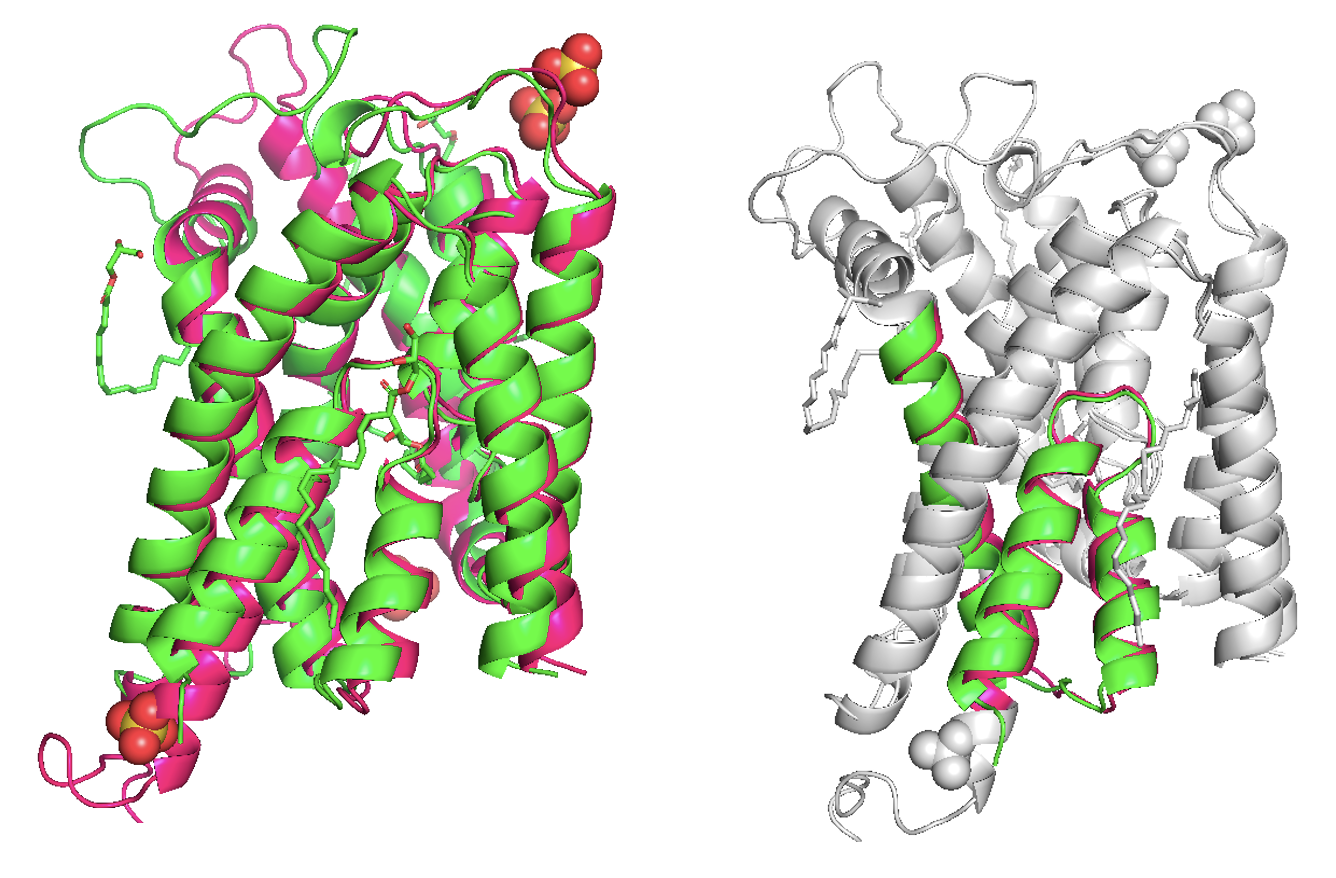
\includegraphics[width=\textwidth]{Results/6cb2_models.png}
    \caption{6cb2 Models}
    \label{fig:6cb2_super}
    \small
    The crystal structure in green and the trRosetta model in magenta.  The second image highlights the re-entrant structural motif feature that became prominent during the course of this investigation. 
\end{figure}


\subsection{Dataset for custom re-entrant sequence database}
A library of re-entrant loop sequences together with the putative re-entrant loop sequences from the Mt2055, Tmem41b and YqjA models were clustered to establish any visible relationships of the sequences. The library was built by obtaining a non-redundant set of 56 re-entrant helix sequences by first retrieving all 714 TM proteins that contain at least one re-entrant loop from the PDBTM \cite{Kozma2012} and removing redundancy with a 40\% identity threshold. The resulting 127 protein structures were split into their component chains, eliminating any chain lacking a re-entrant loop. The resulting set of 188 unique re-entrant loop sequences were then filtered removing any sequences of less than 10 residues and more than 20, thereby ensuring the collection of sequences conformed to the length of typical \cite{Yan2010} re-entrant loops. The remaining 56 sequences were clustered, supplemented by candidate re-entrant sequences from the proteins studied here. Clustering was performed using CLANS v1.0 \cite{Frickey2004} with the BLAST \cite{Altschul1997} results used to calculate strengths of similarity.

\subsection{Dataset for custom structural re-entrant database}
In addition to the construction of the re-entrant sequence database a structural database was also built for the re-entrant loops in the PDBTM. A library of re-entrant loop pdb structures together with the putative re-entrant loop structures from the Mt2055, Tmem41b and YqjA protein models were clustered on their structural similarity. The library was built by obtaining a non-redundant (removing redundancy with a 40\% sequence identity threshold) set of 125 chains from the PDBTM \cite{Kozma2012} that contain at least one re-entrant loop. 40\% sequence identity threshold is considered to be a reasonably stringent criterion for redundancy removal. It ensures that the retained homologues have a significant level of similarity with the query sequence, indicating a high likelihood of shared evolutionary ancestry and potential functional conservation. As this investigation focuses on re-entrant loops that are immediately preceded by a TM helix that is packed against the loop, all re-entrant loops (boundaries defined by PDBTM) in addition to the preceding 30 residues were extracted. The resulting 193 library entries, supplemented with the re-entrant loop features (defined by the OMP server \cite{Lomize2012} and accompanied by the preceding 30 residues) from the ab initio modelling underwent an all-against-all structural alignment using a local installation of Dali v4.0 \cite{Holm2016}. The Z-scores for these alignments were then used for clustering with CLANS v1.0 \cite{Frickey2004} with a Z-score of 4.5 used as the cut-off threshold.

\section{Sequence Analysis}
HHpred \cite{Zimmermann2018} was used to screen a selection of DedA proteins against the Pfam database \cite{El-Gebali2019}. Hits were observed in the same region against both PF09335 and the Pfam domain PF06695 (‘Sm{\_}multidrug{\_}ex’) which is strongly indicative of homology: a probability of 99.4\% with an E-value of 9E-17 for the PF09335 hit and 98.3\% and 2E-10 respectively for PF06695. An HHpred search against the Pfam database using a member of PF06695 - the short archaeal sequence Mt2055 (UniProt code W9DY28) \cite{Apweiler2004} - returned similar results (Table \ref{table:hhpred} ). Figure \ref{fig:msa} shows the MSA for the same sequences along with the relative positions of the two Pfam domains under investigation.  The Mt2055 sequence originates from the unpublished draft genome of the archaebacterium Methanolobus tindarius DSM 2278.  For many of the subsequent analyses, the shorter archaeal sequence was used initially but the clear homology among this set of proteins means that inferences can be drawn across the group.

\begin{table}[]
\caption{HHpred results for Tmem41b and homologues demonstrate homology between Pfam families PF09335 and PF06695.}
\centering
\resizebox{\columnwidth}{!}{%
\begin{tabular}{llllllll}
\rowcolor[HTML]{BDCCD4} 
\multicolumn{2}{l}{\cellcolor[HTML]{BDCCD4}{\color[HTML]{666666} \textbf{}}}                                                  & \multicolumn{2}{l}{\cellcolor[HTML]{BDCCD4}{\color[HTML]{666666} \textbf{}}}                                                    & \multicolumn{2}{l}{\cellcolor[HTML]{BDCCD4}{\color[HTML]{666666} \textbf{\begin{tabular}[c]{@{}l@{}}PF09335\\ 'SNARE\_ASSOC'/ \\ ‘VTT ‘/’Tvp38’\end{tabular}}}} & \multicolumn{2}{l}{\cellcolor[HTML]{BDCCD4}{\color[HTML]{666666} \textbf{\begin{tabular}[c]{@{}l@{}}PF06695\\ ‘Sm\_multidrug\_ex’\end{tabular}}}} \\
\rowcolor[HTML]{BDCCD4} 
{\color[HTML]{666666} \textbf{}} & {\color[HTML]{666666} \textbf{Species}}                                                    & {\color[HTML]{666666} \textbf{\begin{tabular}[c]{@{}l@{}}UniProt\\ Code\end{tabular}}} & {\color[HTML]{666666} \textbf{Length}} & {\color[HTML]{666666} \textbf{Probability}}                                          & {\color[HTML]{666666} \textbf{E-Value}}                                         & {\color[HTML]{666666} \textbf{Probability}}                                   & {\color[HTML]{666666} \textbf{E-Value}}                                  \\
\rowcolor[HTML]{FFFFFF} 
{\color[HTML]{666666} Tmem41b}   & {\color[HTML]{666666} \begin{tabular}[c]{@{}l@{}}Homo \\ sapiens\end{tabular}}             & {\color[HTML]{666666} Q5BJD5}                                                          & {\color[HTML]{666666} 291}             & {\color[HTML]{666666} 99.4}                                                   & {\color[HTML]{666666} 9E-17}                                                    & {\color[HTML]{666666} 98.3}                                            & {\color[HTML]{666666} 2E-10}                                             \\
\rowcolor[HTML]{E5EBEF} 
{\color[HTML]{666666} Ydjx}      & {\color[HTML]{666666} \begin{tabular}[c]{@{}l@{}}Escherichia \\ coli\end{tabular}}         & {\color[HTML]{666666} P76219}                                                          & {\color[HTML]{666666} 236}             & {\color[HTML]{666666} 99.6}                                                   & {\color[HTML]{666666} 2.1E-17}                                                  & {\color[HTML]{666666} 99.1}                                            & {\color[HTML]{666666} 9.9E-13}                                           \\
\rowcolor[HTML]{FFFFFF} 
{\color[HTML]{666666} Ydjz}      & {\color[HTML]{666666} \begin{tabular}[c]{@{}l@{}}Escherichia \\ coli\end{tabular}}         & {\color[HTML]{666666} P76221}                                                          & {\color[HTML]{666666} 235}             & {\color[HTML]{666666} 99.6}                                                   & {\color[HTML]{666666} 1.1E-17}                                                  & {\color[HTML]{666666} 99.0}                                            & {\color[HTML]{666666} 4.5E-16}                                           \\
\rowcolor[HTML]{E5EBEF} 
{\color[HTML]{666666} Yqja}      & {\color[HTML]{666666} \begin{tabular}[c]{@{}l@{}}Escherichia \\ coli\end{tabular}}         & {\color[HTML]{666666} P0AA63}                                                          & {\color[HTML]{666666} 220}             & {\color[HTML]{666666} 99.62}                                                  & {\color[HTML]{666666} 5.6E-15}                                                  & {\color[HTML]{666666} 99.41}                                           & {\color[HTML]{666666} 1.3E-12}                                           \\
\rowcolor[HTML]{FFFFFF} 
{\color[HTML]{666666} Tvp38}     & {\color[HTML]{666666} \begin{tabular}[c]{@{}l@{}}Saccharomyces \\ cerevisiae\end{tabular}} & {\color[HTML]{666666} P36164}                                                          & {\color[HTML]{666666} 337}             & {\color[HTML]{666666} 99.4}                                                   & {\color[HTML]{666666} 7.9E-15}                                                  & {\color[HTML]{666666} 98.7}                                            & {\color[HTML]{666666} 2.7E-10}                                           \\
\rowcolor[HTML]{E5EBEF} 
{\color[HTML]{666666} Mt2055}    & {\color[HTML]{666666} \begin{tabular}[c]{@{}l@{}}Methanolobus \\ tindarius\end{tabular}}   & {\color[HTML]{666666} W9DY28}                                                          & {\color[HTML]{666666} 168}             & {\color[HTML]{666666} 99.0}                                                   & {\color[HTML]{666666} 2.4E-10}                                                  & {\color[HTML]{666666} 99.8}                                            & {\color[HTML]{666666} 1.8E-20}                                          
\end{tabular}
}
\label{table:hhpred}
\end{table}

\begin{figure}[th!]
    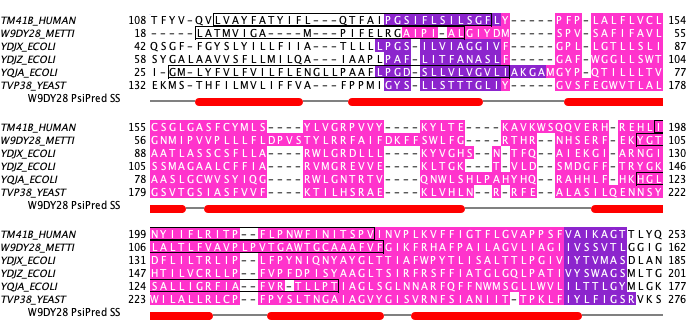
\includegraphics[width=\textwidth]{Results/fig1.png}
    \caption{MSA for query protein selection listed in table \ref{table:hhpred}.}
    \label{fig:msa}
    \small
    Magenta highlights the regions matched by HHpred to the PF06695 Pfam domain while purple is used for additional residues included in the PF09335 Pfam domain matches. The black boxed regions represent the locations of the putative re-entrant loops as identified by the modeling of the respective proteins. The secondary structure for the archaeal W9DY29 sequence (Mt2055) is also depicted with the relative positions of alpha helices shown as red blocks.
\end{figure}

There are no known experimental protein structures representing PF09335 or PF06695, but both Gremlin and DMPfold have constructed ab initio models for these Pfam domains and have made them available in repositories \cite{Greener2019, Ovchinnikov2017}.

Analysis of the HHpred results obtained for the archaeal protein Mt2055 revealed the presence of additional hits for both PF06695 and PF09335 Pfam domains, in which the C-terminal half of the domains aligned with the N-terminal half of the Archaea protein. For example, residues 1-69 of the archaeal protein aligned with residues 52-117 of the Pfam PF09335 profile with a probability of 74.15\%.

Interestingly, contact density analysis \cite{Rigden2002}\cite{Sadowski2013} supported the existence of a domain boundary around residue 60, in broad agreement with the HHpred results (Figure \ref{fig:w9_dom_anal}). Both the HHpred and contact density results therefore pointed to a specific domain structure being present.

\begin{figure}[th!]
    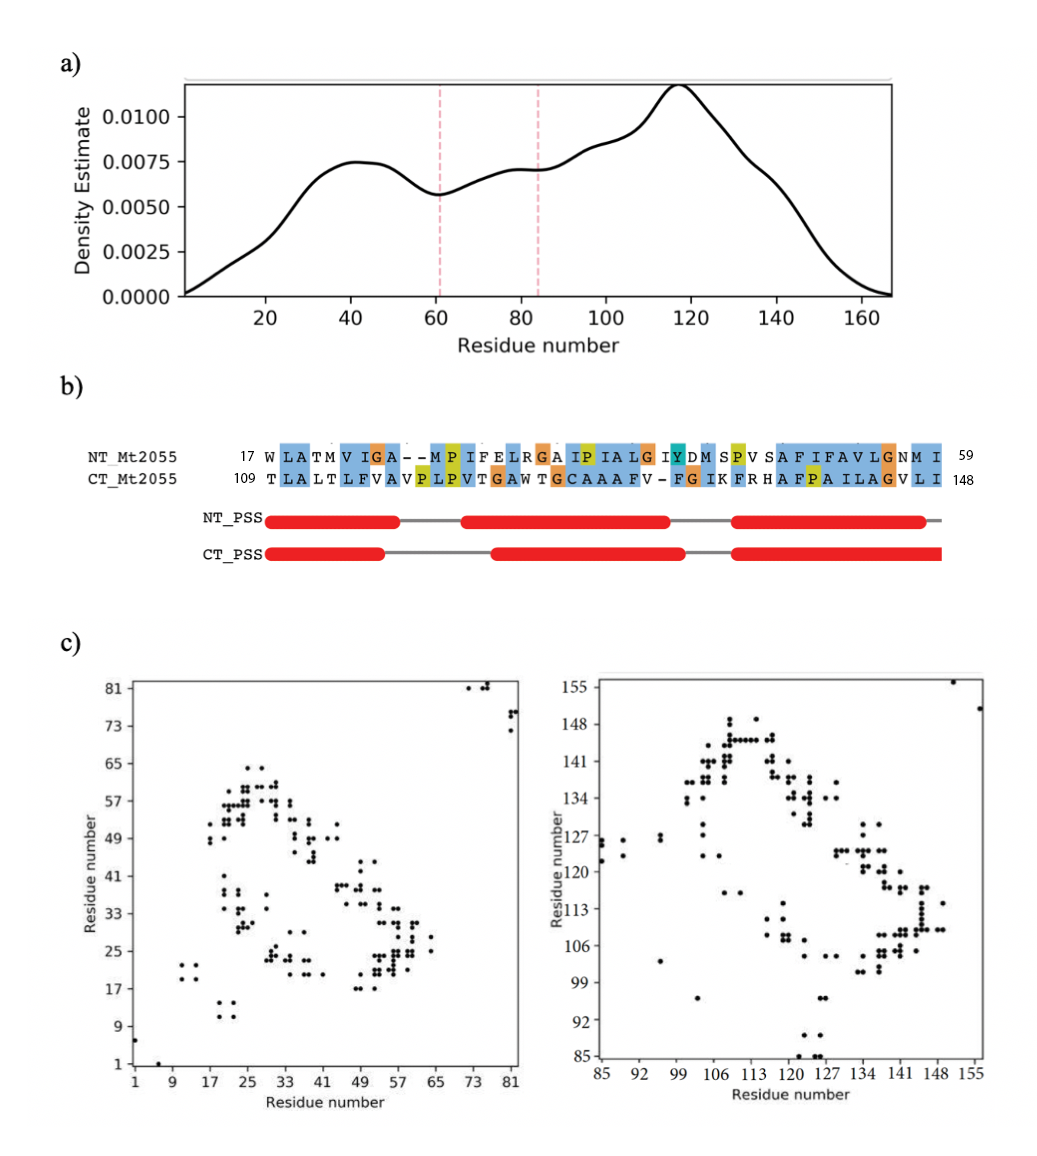
\includegraphics[width=\textwidth]{Results/fig2.png}
    \caption{Mt2055 domain analysis. }
    \label{fig:w9_dom_anal}
    \small
    (a) Contact density profile constructed by ConKit \cite{Simkovic2017} utilising DeepMetaPSICOV contact prediction. Solid black line represents contact density and dotted red lines mark density minima corresponding to possible domain boundaries. (b) HHalign alignments for the N-terminal and C-terminal Mt2055 halves, formatted using Jalview \cite{Waterhouse2009} and coloured according to the ClustalX \cite{jeanmougin1998multiple} scheme. Red bars represent helical secondary structure. (c) Maps of predicted contacts generated by DeepMetaPSICOV \cite{Kandathil2019} and plotted using ConKit \cite{conkit2017}; left is N-terminal half (residues 1-84) and right is C-terminal half (residues 85-168). Black points represent predicted intramolecular contacts.
\end{figure}

When the Mt2055 sequence was split at residue 60-61, the resulting N-terminal region of 60 residues and the C-terminal section of 79 residues could be aligned using HHalign \cite{Soding2005} with a 78\% probability and an E-value of 1.9E-3. Examination of the map of predicted contacts for Mt2055 reveals features that are present in both the N- and C-terminal halves of the protein (Figure \ref{fig:w9_dom_anal}c). Taken together, these data strongly support the existence of a tandem repeat within the Mt2055 protein and hence across the PF06695 and PF09335 protein families.\\
Interestingly, an equivalent sequence analysis with HHpred of other PF09335 homologues including Tmem41b itself does not reveal a repeat. However, inspection of their corresponding predicted contact maps does reveal features repeated when N- and C-halves of the protein are compared (Figure \ref{fig:tm_c_map}). Apparently, evolutionary divergence has removed all trace of the repeat sequence signal in bacterial and eukaryotic proteins, although the feature remains visible by evolutionary covariance analysis.\\

In order to assess the composition of the repeat identified, transmembrane helical topology predictions were carried out but gave inconsistent results for most proteins: only for the archaeal protein Mt2055 did all methods agree that four transmembrane helices were predicted to be present in the whole protein, two in each of the repeats (Table \ref{table:tm_pred}).

\begin{table}
\caption{Predicted number of TM regions for PF09335/PF06695 homologs}
\resizebox{\columnwidth}{!}{%
\centering
\begin{tabular}{lccccccc}
\rowcolor[rgb]{0.753,0.753,0.753} ~         & \multicolumn{1}{l}{TOPCONS} & \multicolumn{1}{l}{OCTOPUS} & \multicolumn{1}{l}{PHILIUS} & \multicolumn{1}{l}{POLYPHOBIUS} & \multicolumn{1}{l}{SCAMPI} & \multicolumn{1}{l}{SPOCTOPUS} & \multicolumn{1}{l}{TMHMM}  \\
{\cellcolor[rgb]{0.753,0.753,0.753}}Mt2055  & 4                           & 4                           & 4                           & 4                               & 4                          & 4                             & 4                          \\
{\cellcolor[rgb]{0.753,0.753,0.753}}Tmem41b & 6                           & 6                           & 6                           & 7                               & 6                          & 5                             & 6                          \\
{\cellcolor[rgb]{0.753,0.753,0.753}}Ydjx    & 7                           & 7                           & 5                           & 6                               & 6                          & 7                             & 5                          \\
{\cellcolor[rgb]{0.753,0.753,0.753}}Ydjz    & 6                           & 7                           & 6                           & 6                               & 6                          & 6                             & 5                          \\
{\cellcolor[rgb]{0.753,0.753,0.753}}Tvp38   & 5                           & 7                           & 5                           & 7                               & 6                          & 6                             & 5                         
\end{tabular}
}
\label{table:tm_pred}
\end{table}

\begin{figure}[th!]
    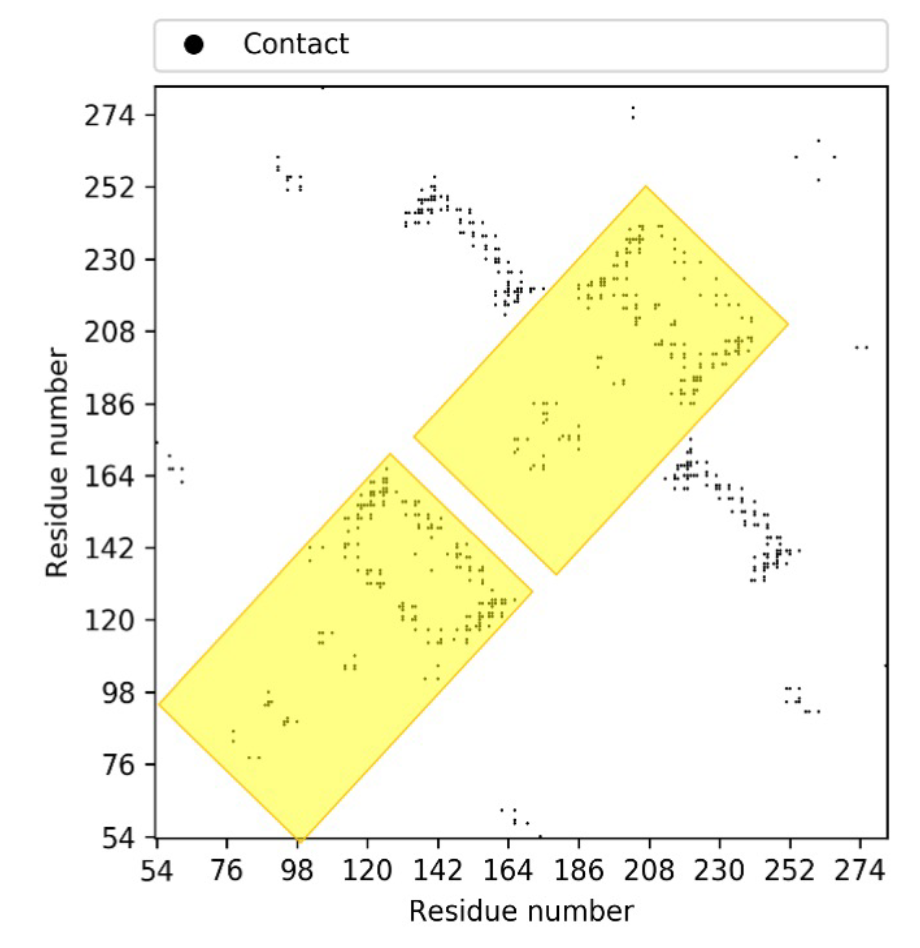
\includegraphics[width=\textwidth]{Results/fig3.png}
    \caption{Tmem41b Contact map constructed using DeepMetaPSICOV and plotted using Conkit.}
    \label{fig:tm_c_map}
    \small
    The highlighted areas represent repeat units that have been revealed through evolutionary covariance analysis.
\end{figure}

Several authors have deposited structures of uncharacterised Pfam families in databases \cite{El-Gebali2019}; however, Pfam domain boundaries for PF09335/PF06695, which define the limits of these previous modelling exercises, do not reflect the conserved structural domain that we predict. Given the fact that the available ab initio models were inconsistent with the transmembrane helix topology, secondary structure and contact predictions, new models of Mt2055 as well as Tmem41b and YqjA were built. 

\section{Initial Modelling}
Initial modelling of DedA proteins centered around constructing DeepContact \cite{Liu2018} derived contact restrained Mt2055 models using Rosetta \emph{ab initio}.  The output models were visually of very poor quality and could not possibly be stable within a membrane.  Subsequently, in an effort to improve the quality of the contact information a metagenomics \cite{Ovchinnikov2017} sequence database was used to generate the predicted contacts.  The MapPred \cite{wu2020protein} server was used to trial the use of metagnomics; for Mt2055 the Neff of the MSA was raised to 2687 from the  1648 Uniprot-derived MSA; for Tmem41b the Neff of the MSA was raised to 8874 from the 2144 Uniprot derived MSA.  The success at raising the Neff values of the MSAs for the query proteins led to the construction of a custom metagenomics sequence database. JackHMMER \cite{Johnson2010} was used to generate the MSAs and ResPre \cite{Li} to make the contact predictions based on the metagenomics enhanced MSAs.  With the custom metagenomics database, for Mt2055 the Neff reached 7470 and for Tmem41b the Neff increased to 88573.  Figure \ref{fig:seq_coverage} shows how the increase in Neff translated to local sequence regions  with the use of series of sequence coverage plots generated using ConKit \cite{conkit2017}; for example for Tmem41b, even though the metagenomic improved the global Neff score dramatically, the MSA coverage profile does highlight the fact that the metegenomics has little impact on the first one hundred residues.

\begin{figure}[th!]
    \makebox[\textwidth]{\includegraphics[width=\paperwidth]{...}}
    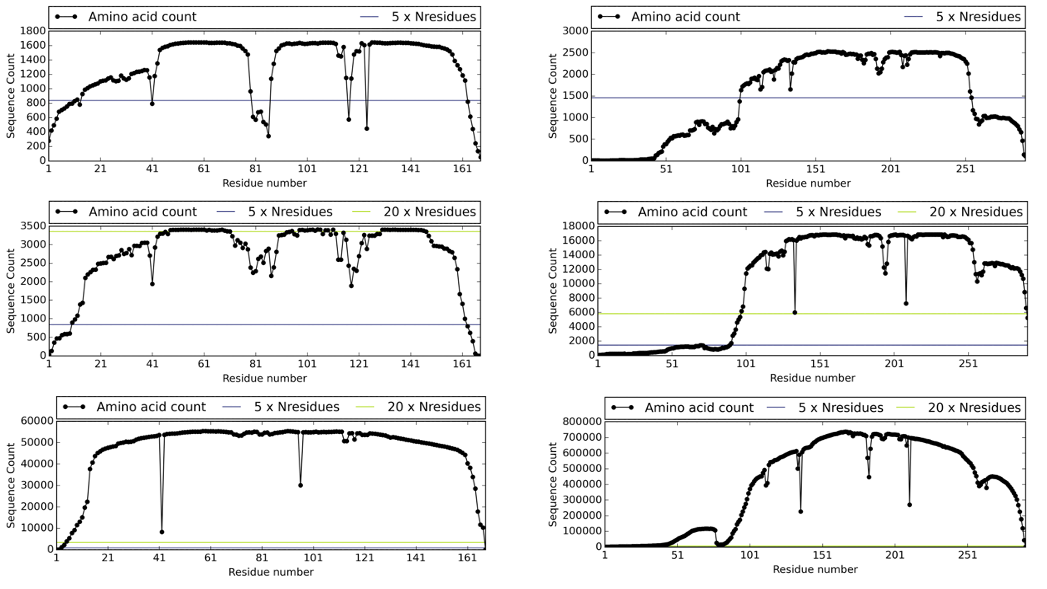
\includegraphics[width=\textwidth]{Results/meta_fig.png}
    \caption{MSA Sequence coverage profiles.}
    \label{fig:seq_coverage}
    \small
    Column 1: Mt2055, Column 2: Tmem41b, Row 1: Uniprot derived, Row 2: MapPred derived, Row 3: Custom metagenomics database derived.
\end{figure}

Again, even with the metagenomic enhanced contact predictions, the poor model quality could be visually identified (short transmembrane helices -less than 5 helical turns- that could not possibly span the lipid bi-layer) and quantitatively measured using a contact satisfaction profile plotted using ConKit (figure \ref{fig:precision}).  Running these models as well as the examples from the previous set against the PDB using Dali \cite{Holm2016} to identify possible stuructural homologues did not yield any significant results with the top Z-score being 3.5.

\begin{figure}[th!]
    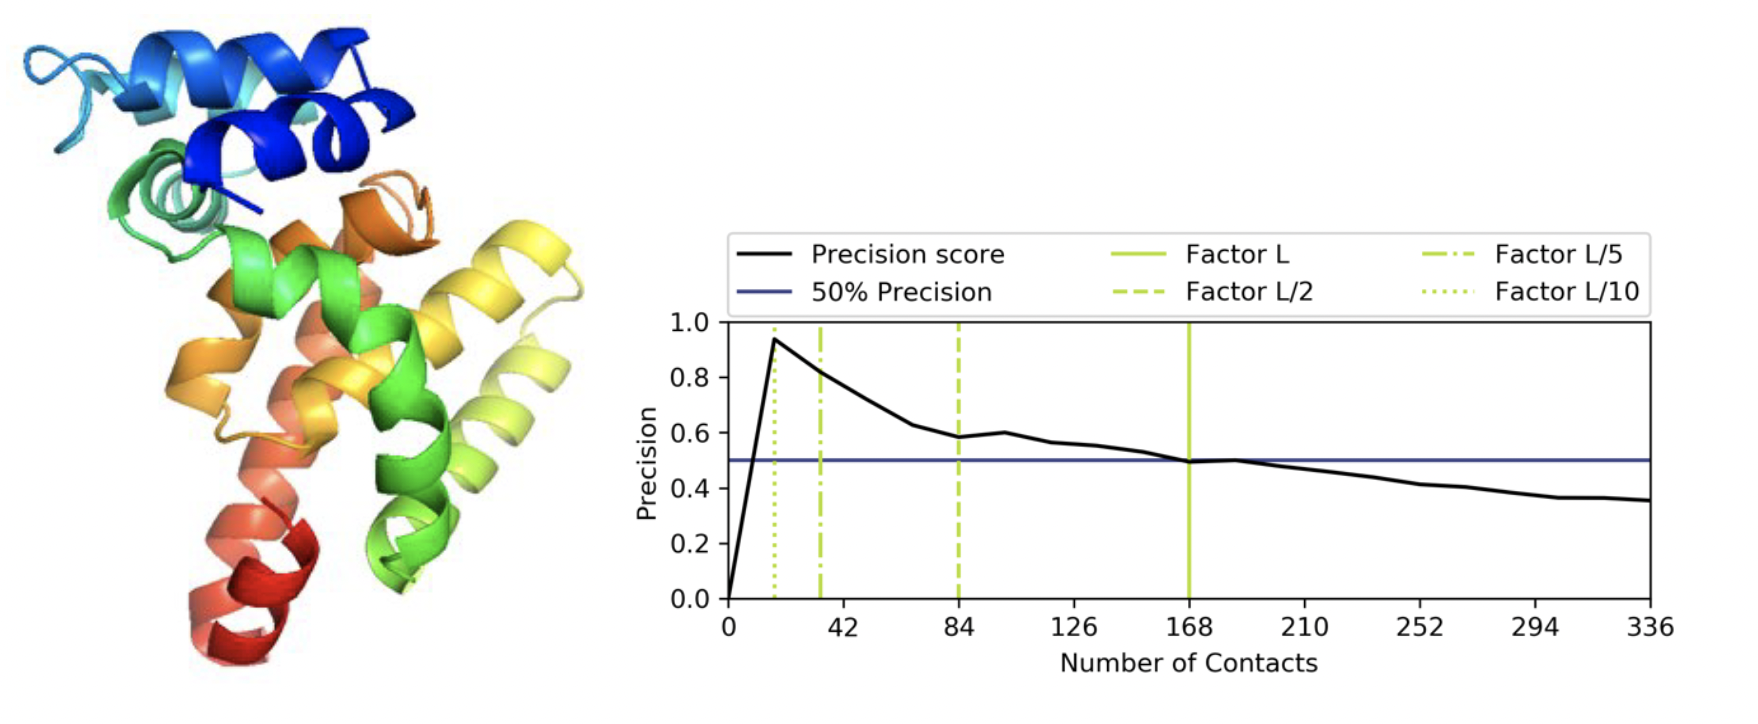
\includegraphics[width=\textwidth]{Results/meta_ros_model_fig.png}
    \caption{Rosetta Ab initio model with Precision Profile.}
    \label{fig:precision}
    \small
    Left: Mt2055 Rosetta ab initio model utilising restraints derived from Respre (Li et al.,
n.d.) and a metagenomic database for MSA construction; coloured with rainbow; blue C -terminal
to red N-terminal; right: precision profile depicting contact satisfaction at various contact cutoff values where L = sequence length (rounded down to the nearest whole number of contacts). The 50\% precision cut of is shown (blue line) as a visual marker. A minimum of 70\% contact satisfaction for the top L contacts would be suggestive of good quality models \cite{de2017comparing}..
\end{figure}

Building on the premise of utilising the contacts as restraints in the model making, it was decided to switch to the Rosetta Ab initio Membrane protocol \cite{alford2015integrated}.  This version of Rosetta \textit{ab initio}, in addition to the contact derived restraints, uses membrane topology predictions as further restraints and are more heavily weighted than the contact information.  TopCons \cite{Tsirigos2015} was used to generate the membrane topology predictions for the query proteins which were subsequently converted into the Rosetta Membrane compatible OCTOPUS \cite{Viklund2008} format.\\

One thousand models were constructed. The output models from the RosettaMembrane flavour were visually superior to the outputs from Rosetta ab initio;  these models possessed helices packed together in such a way that they could conceivably sit in a membrane bi-layer.  Screening the highest ranking model (centroid of the largest cluster determined by SPICKER \cite{Zhang2004}) against the PDB using DALI and filtering out globular proteins and all hits with a Z-score less than 5 resulted in a list of strong hits with Type VII ABC transporters (Table \ref{table:abc}) with the strongest hit against 5lilA (Figure \ref{fig:5lil_super}). \\

In an effort to identify a potentially stronger hit from the one thousand models, the set of models were processed into a local DALI database and 5lilA was used to query the library.  However, the same model with a Z-score of 8.8 was picked out.  Consequently a further ten thousand RosettaMembrane models were constructed and 5lil was screened against this new model set.  A model with a Z-score of 9.9 was identified.

\begin{table}
\caption{DALI PDB hits with top model from first round of RosettaMembrane modelling}
\resizebox{\columnwidth}{!}{%
\centering
\begin{tabular}{lllllll}
\rowcolor{cyan} Hit                  & Z-Score & RMSD & lali & Nres & \%ID & Hit Name                                           \\
\rowcolor[rgb]{0.137,1,0.769} 5lil-A & 8.8     & 3.8  & 131  & 615  & 12   & MACROLIDE EXPORT ATP-BINDING/PERMEASE PROTEIN MAC  \\
\rowcolor{cyan} 5lj6-A               & 8.3     & 5    & 132  & 600  & 8    & MACROLIDE EXPORT ATP-BINDING/PERMEASE PROTEIN MAC  \\
\rowcolor[rgb]{0.137,1,0.769} 5lj7-B & 8       & 4.9  & 132  & 599  & 8    & MACROLIDE EXPORT ATP-BINDING/PERMEASE PROTEIN MAC  \\
\rowcolor{cyan} 5lil-B               & 7.1     & 4.9  & 132  & 604  & 8    & MACROLIDE EXPORT ATP-BINDING/PERMEASE PROTEIN MAC  \\
\rowcolor[rgb]{0.137,1,0.769} 5mal-A & 7       & 3.9  & 104  & 234  & 14   & LIPASE;                                            \\
\rowcolor{cyan} 5lj7-A               & 6.7     & 4    & 125  & 592  & 11   & MACROLIDE EXPORT ATP-BINDING/PERMEASE PROTEIN MAC  \\
\rowcolor[rgb]{0.137,1,0.769} 5mal-B & 6.6     & 3.5  & 103  & 234  & 15   & LIPASE;                                            \\
\rowcolor{cyan} 5ws4-B               & 6.4     & 4    & 129  & 650  & 8    & MACROLIDE EXPORT ATP-BINDING/PERMEASE PROTEIN MAC  \\
\rowcolor[rgb]{0.137,1,0.769} 6fpf-A & 6.3     & 3.9  & 125  & 257  & 6    & CHROMOSOME 16, WHOLE GENOME SHOTGUN SEQUENCE;      \\
\rowcolor{cyan} 5ws4-A               & 6.3     & 4    & 129  & 650  & 8    & MACROLIDE EXPORT ATP-BINDING/PERMEASE PROTEIN MAC  \\
\rowcolor[rgb]{0.137,1,0.769} 5gtm-B & 6.2     & 6.2  & 92   & 522  & 12   & INTERFERON-INDUCED GTP-BINDING PROTEIN MX1;        \\
\rowcolor{cyan} 5nil-J               & 6.1     & 4.2  & 131  & 629  & 13   & OUTER MEMBRANE PROTEIN TOLC;                       \\
\rowcolor[rgb]{0.137,1,0.769} 5nik-J & 6.1     & 4.2  & 131  & 629  & 13   & OUTER MEMBRANE PROTEIN TOLC;                       \\
\rowcolor{cyan} 5gko-B               & 6.1     & 3.8  & 126  & 650  & 8    & MACROLIDE EXPORT ATP-BINDING/PERMEASE PROTEIN MAC  \\
\rowcolor[rgb]{0.137,1,0.769} 5nik-K & 5.9     & 4.4  & 133  & 629  & 12   & OUTER MEMBRANE PROTEIN TOLC;                       \\
\rowcolor{cyan} 5nil-K               & 5.9     & 4.4  & 133  & 629  & 12   & OUTER MEMBRANE PROTEIN TOLC;                       \\
\rowcolor[rgb]{0.137,1,0.769} 5do7-C & 5.8     & 5.3  & 129  & 579  & 7    & ATP-BINDING CASSETTE SUB-FAMILY G MEMBER 5;       
\end{tabular}
}
\label{table:abc}
\end{table}

\begin{figure}[th!]
    \centering
    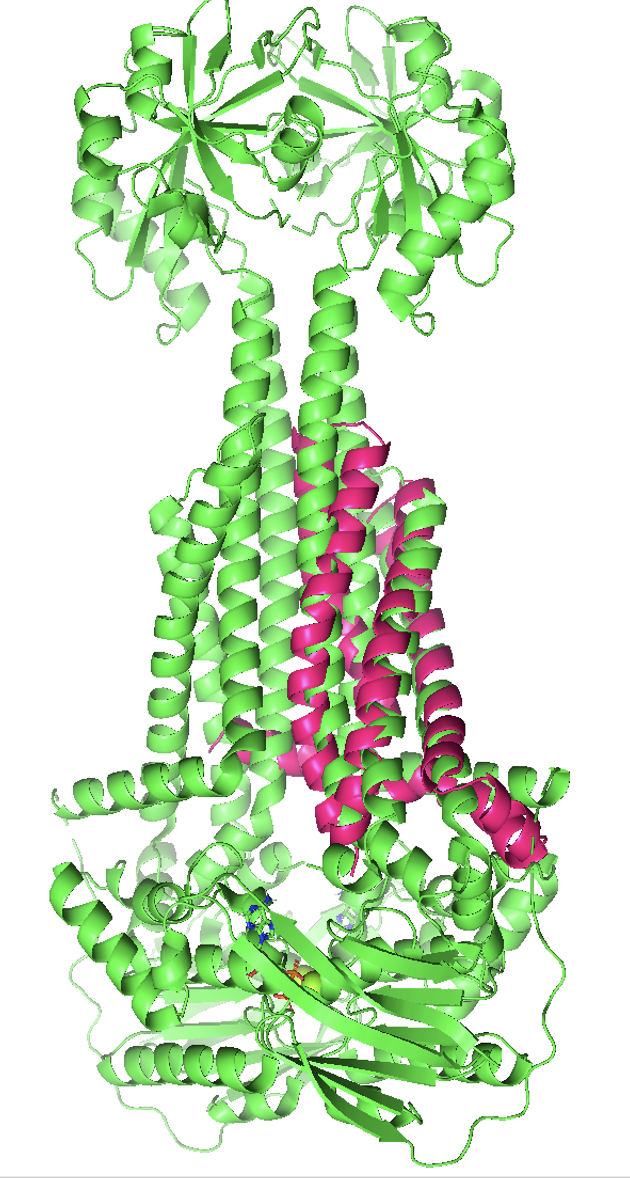
\includegraphics[width=50mm, scale =0.5]{Results/5lil_super_fig.png}
    \caption{Rosetta Membrane model structurally aligned with 5lilA.}
    \label{fig:5lil_super}
    \small
    Rosetta Ab initio Membrane model (magenta) structurally aligned with 5lil (green).
\end{figure}

Next the idea of refining the model based on use of contact restraints was experimented with; the contacts from the model with the highest alignment Z-score with 5lil were used as restraints to construct a further ten thousand new models.  The output models were again converted to a DALI database and 5lil was screened against the new library.  This additional refinement step did not produce models with any higher alignment scores with 5lil.  A comparison of the 5lil contact map and the model contact map \ref{fig:5lil_cmaps} clearly showed that they certainly shared the transmembrane helical topology.  Study of the structural alignment (figure \ref{fig:5lil_schem}) also confirmed this. Additionally, both the model and 5lil possessed an amphipathic helix, albeit in the opposite direction (although this would not have contributed to the DALI Z-score calculation as only the aligned regions are used for this calculation).\\

5lil was an interesting structural hit. The fold and topology of the MacB transmembrane and periplasmic domain is different from the six other ABC transporter superfamilies and has an independent evolutionary origin from other ABC transporters. 5lil has a four-transmembrane helix topology, periplasmic domain, and stalk.  5lil forms a pump with TolC,  this complex uses cytoplasmic ATP hydrolysis to move substrates from the periplasm to the outside of the cell. 5lil is not considered a transporter as the ATP hydrolysis is used to transmit a conformational changes from cytoplasmic side of the membrane to the periplasmic side; TolC is responsible for the movement of substrate from the periplasm to the outside of the cell. It is the transmembrane domain of 5lil that is responsible for this mechanotransmission \cite{pichoff2019roles}.

\begin{figure}[htb]
    \centering % <-- added
\begin{subfigure}{0.25\textwidth}
  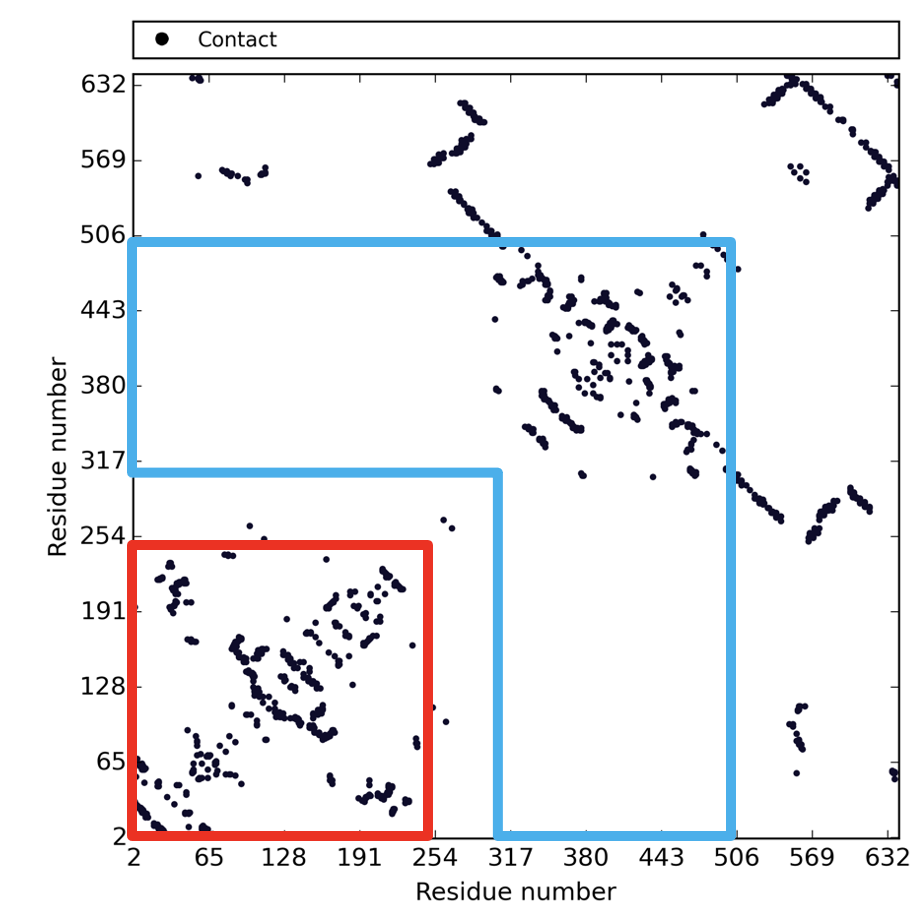
\includegraphics[width=\linewidth]{Results/5lil_1.png}
  \caption{5lilA contact map}
  \label{fig:0}
\end{subfigure}\hfil % <-- added
\begin{subfigure}{0.25\textwidth}
  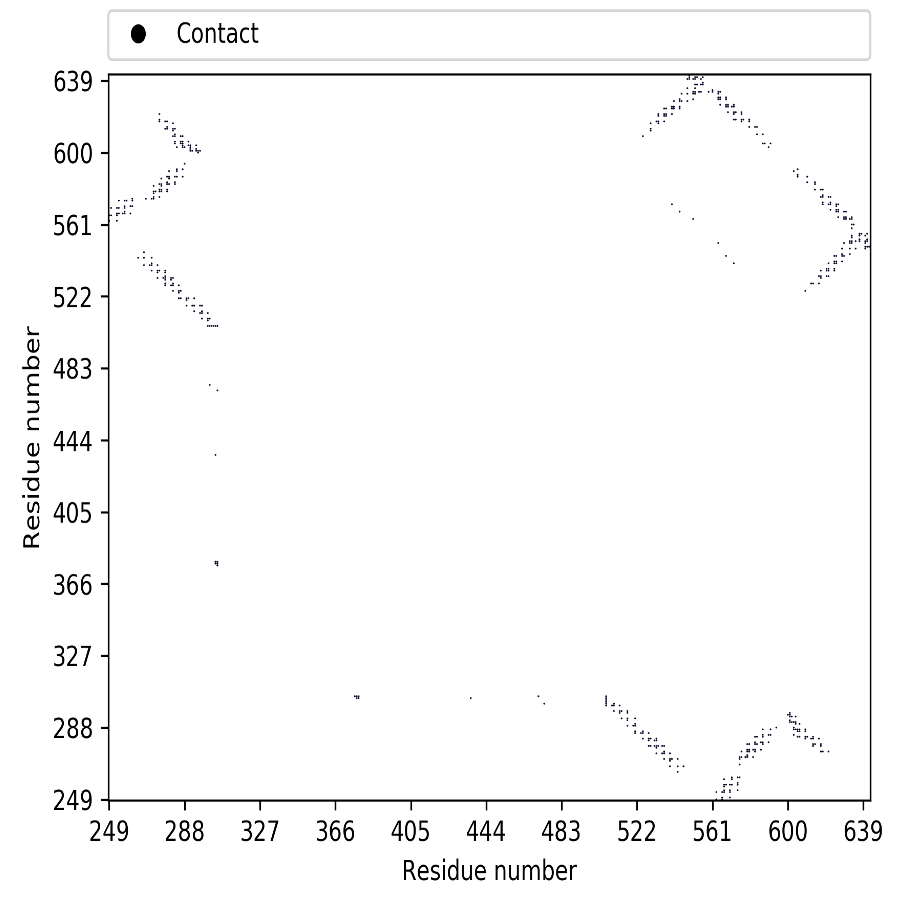
\includegraphics[width=\linewidth]{Results/5lil_2.png}
  \caption{Edited 5lil contact map}
  \label{fig:1}
\end{subfigure}\hfil % <-- added
\begin{subfigure}{0.25\textwidth}
  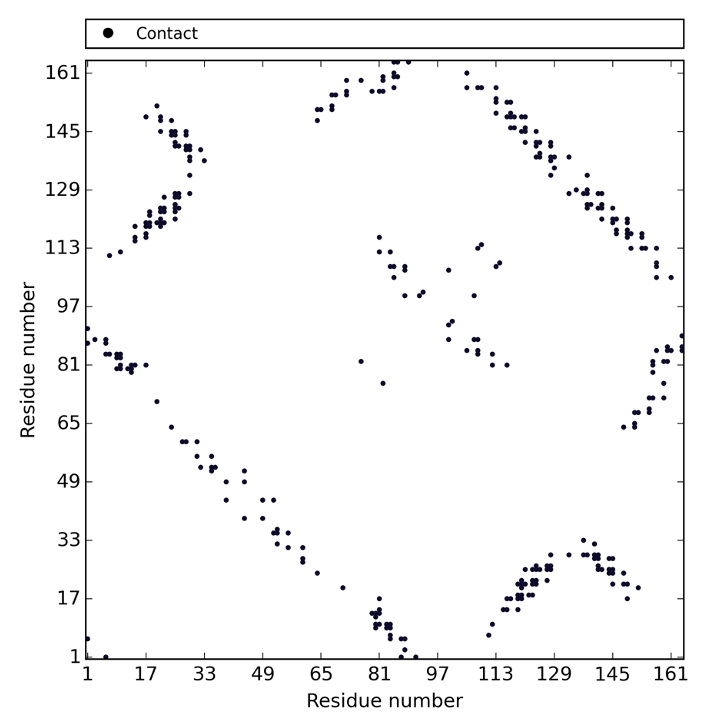
\includegraphics[width=\linewidth]{Results/5lil_topmodel.png}
  \caption{Top model contact map}
  \label{fig:2}
\end{subfigure}
\caption{5lil Contact map analysis}
\small
a) Blue box is periplasmic domain (residues 306-503) and red box is nucleotide binding domain (residues 1-240). b) 5lilA contact map with periplasmic and nucleotide biding domains removed. c) Rosetta membrane top model contact map.
\label{fig:5lil_cmaps}
\end{figure}

\begin{figure}[th!]
    \centering
    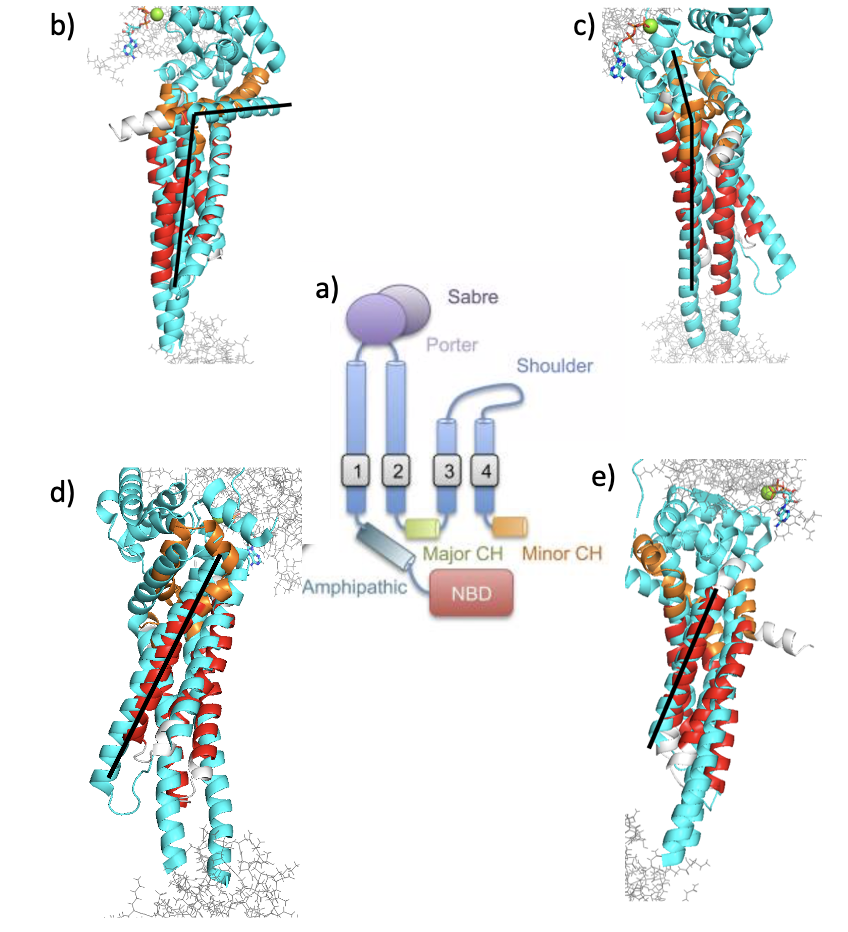
\includegraphics [width=100mm, scale =0.5]{Results/macb_fig.png}
    \caption{Structural alignment analysis of 5lilA and model.}
    \label{fig:5lil_schem}
    \small
    Cartoon: structurally aligned regions; Wire: non aligned regions. cyan: structural aligned region of 5lil; Red: regions of model that are predicted to be transmembrane helices by transmembrane topology prediction tools \ref{table:tm_pred}; Orange: regions of model where there is a lack on consensus between transmembrane topology prediction tools; White: Regions of model that are not predicted to to be transmembrane helices. 
    a)5lilA schmatic (adapted from \cite{pichoff2019roles}). b)Highlighted with a black stick is the alignment of model TM1 with TM1 of 5lilA (involved in dimer formation) along with the presence of the amphipathic helix. c) highlighted with a black stick is the alignment of model TM2 with TM2 of 5lilA (involved in dimer formation) Coupling helix 1 (CH1) (involved in NBD interaction). d)Highlighted with a black stick is the alignment of model TM3 with TM3 of 5lilA. e) Highlighted with a black stick is the alignment of model TM4 with TM4 of 5lilA and Coupling helix 1 (CH2) (involved in NBD interaction). 
\end{figure}

In spite of the fact that the resultant RosettaMembrane models appeared visually more promising; being more in line with transmembrane proteins and having good structural alignments with crystal structures of Type VI ABC transporters; once again when performing quantitative analysis of the ab initio models it resulted in poor precision scores (Figure \ref{fig:5lil_prec}). The unsuccessful modelling attempts lead to the detailed review of all sequence-based prediction data using custom visualisation plots.

\begin{figure}[th!]
    \centering
    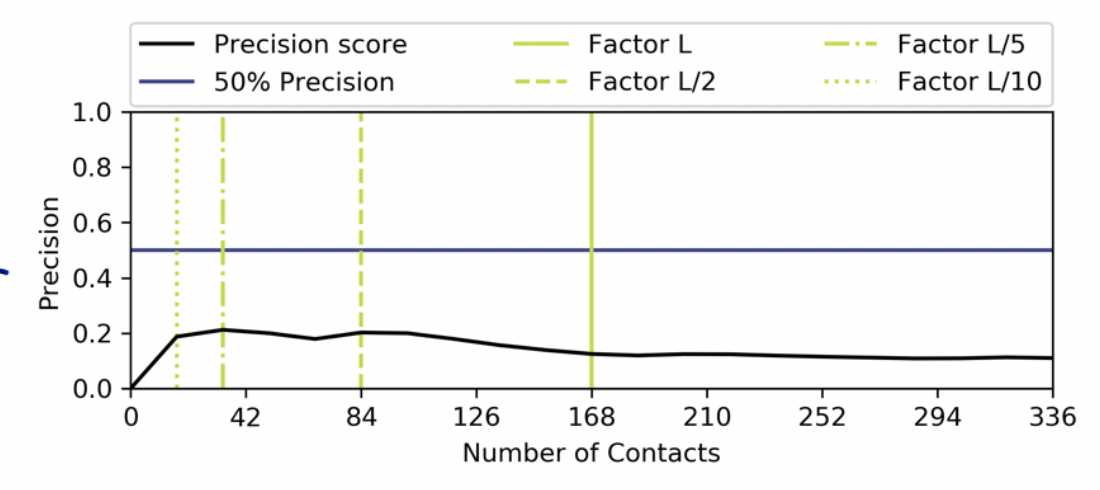
\includegraphics[width=100mm, scale =0.5]{Results/5lil_precision_fig.png}
    \caption{Precision profile for top RosettaMembrane model.}
    \label{fig:5lil_prec}
    \small
    Precision score evaluation of the RosettaMembrane model in relation to the predicted contacts at various contact cutoff values where L = sequence length (rounded down to the nearest whole number of contacts). The 50\% precision cut of is shown (blue line) as a visual marker. A minimum of 70\% contact satisfaction for the top L contacts would be suggestive of good quality models \cite{de2017comparing}.
\end{figure}

\newpage
\section{Development of ConPlot}
The poor precision scores of models built by Rosetta ab initio and RosettaMembrane, along with evidence that the transmembrane topology predictions may contain false positives (Table \ref{table:tm_pred}) led to the desire to visually cross-reference all available prediction data for both Mt2055 and Tmem41b. ConKit \cite{conkit2017}, a python interface to contact predictions, was chosen as a suitable platform to integrate various prediction data. ConKit was already able to output contact predictions in the form of a contact map where the contact predictions are visualised as a two-dimensional binary matrices \cite{godzik1993regularities}.  The contact maps traditionally have a blank space on and near the diagonal axis as they exclude contacts between sequential near neighbours. The ConKit software was adapted to parse other prediction data and output the data in a visual format with the contact map (figure \ref{fig:conplot}). The void in the diagonal of the contact map has been used previously to hold a visualisation of secondary structure information \cite{taylor2016algorithm}.  Various properties can be predicted by other sequence-based methods such as membrane and disorder predictions as well as residue conservation scores.  By integrating this multitude of data a more complete and integrated two-dimensional visual representation of the protein. \\

\begin{figure}[th!]
    \centering
    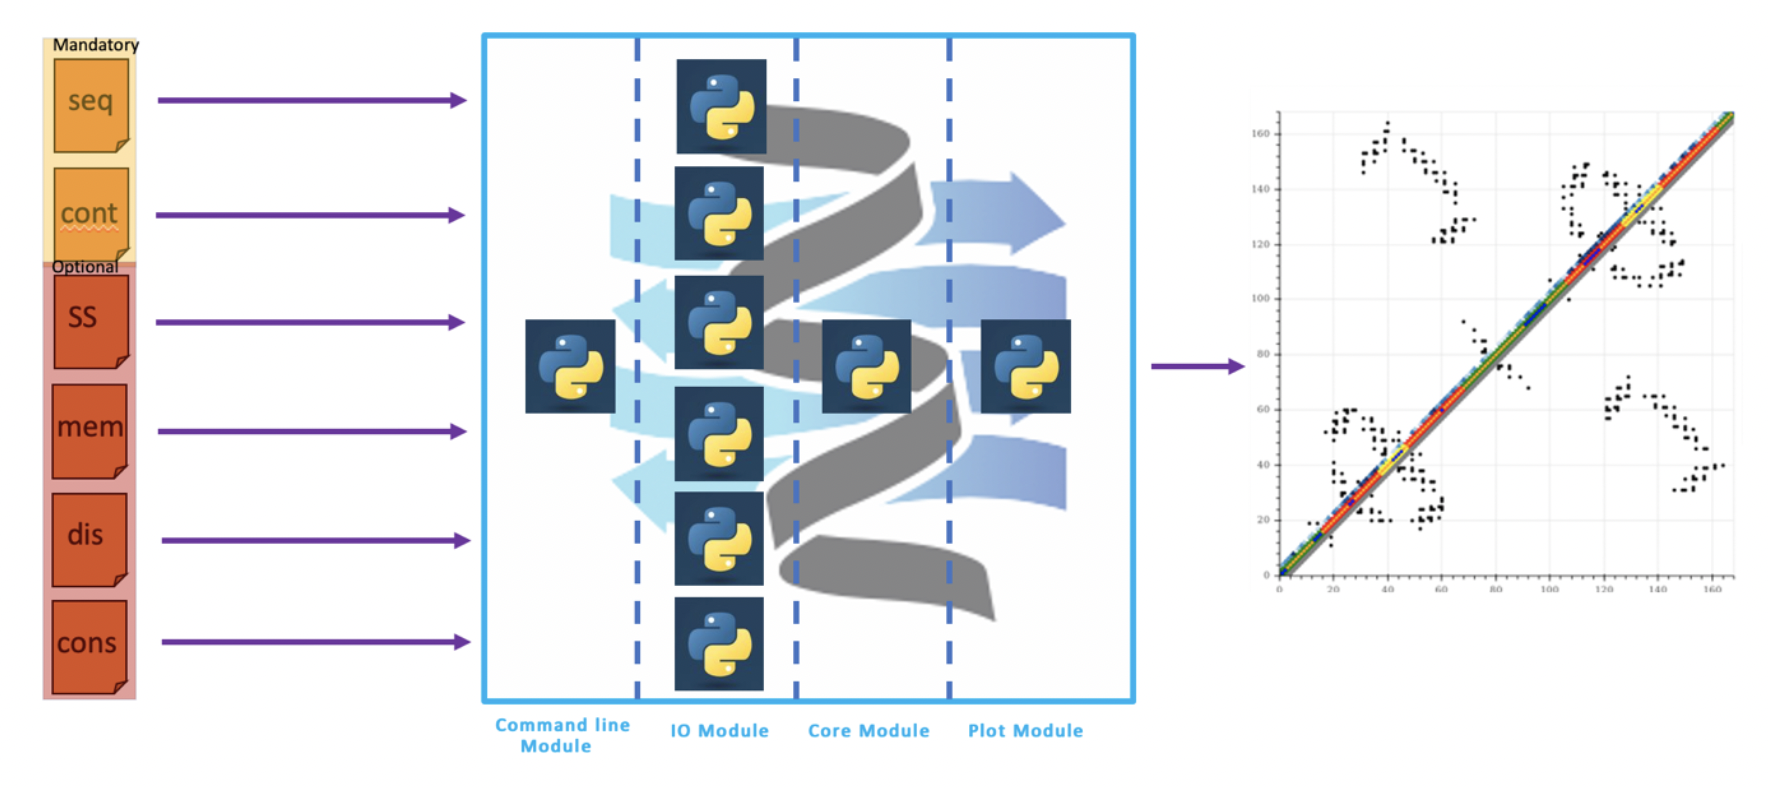
\includegraphics[width=\textwidth]{Results/conkit.png}
    \caption{Integration of new parsers into Conkit.}
    \label{fig:conplot}
    \small
    ConKit flow diagram showing prediction data types (left). Both the sequence data and contact information are mandatory sets of data required to build the data visualisation map; secondary structure (psipred format), membrane prediction (Topcons format), disorder prediction (Iupred2a format) and individual residue conservation scores (consurf format are optional data sets to be processed. New ConKit module scripts (middle) were constructed and integrated into the ConKit software. New output with prediction data visualised on diagonal (right) in the form of an interactive plot.
\end{figure}

New scripts were integrated into the command line, IO, core and plot modules of ConKit. The modifications to ConKit produced the desired output where all available prediction data for a given protein was displayed visually (figure \ref{fig:conplot}). (This visual cross referencing functionality was later developed into the web based application ConPlot \cite{sanchez2021conplot}).

With the visualisation of membrane predictions (TopCons) and secondary structure (PSIPRED) for Mt2055, inspection of the enhanced ConKit output revealed the possible presence of a re-entrant loop structure between residues 16–42 (Figure \ref{fig:w9_enhan_cmap}); a predicted transmembrane region (red) with a break in the centre that separates two distinct predicted helices (blue; from residues 16–25 and 28–42) in contact with each other). The predicted contact map also highlights a second re-entrant loop from residues 105–131, in accordance with the evidence that the protein family resulted from a tandem duplication. 

\begin{figure}[th!]
    \centering
    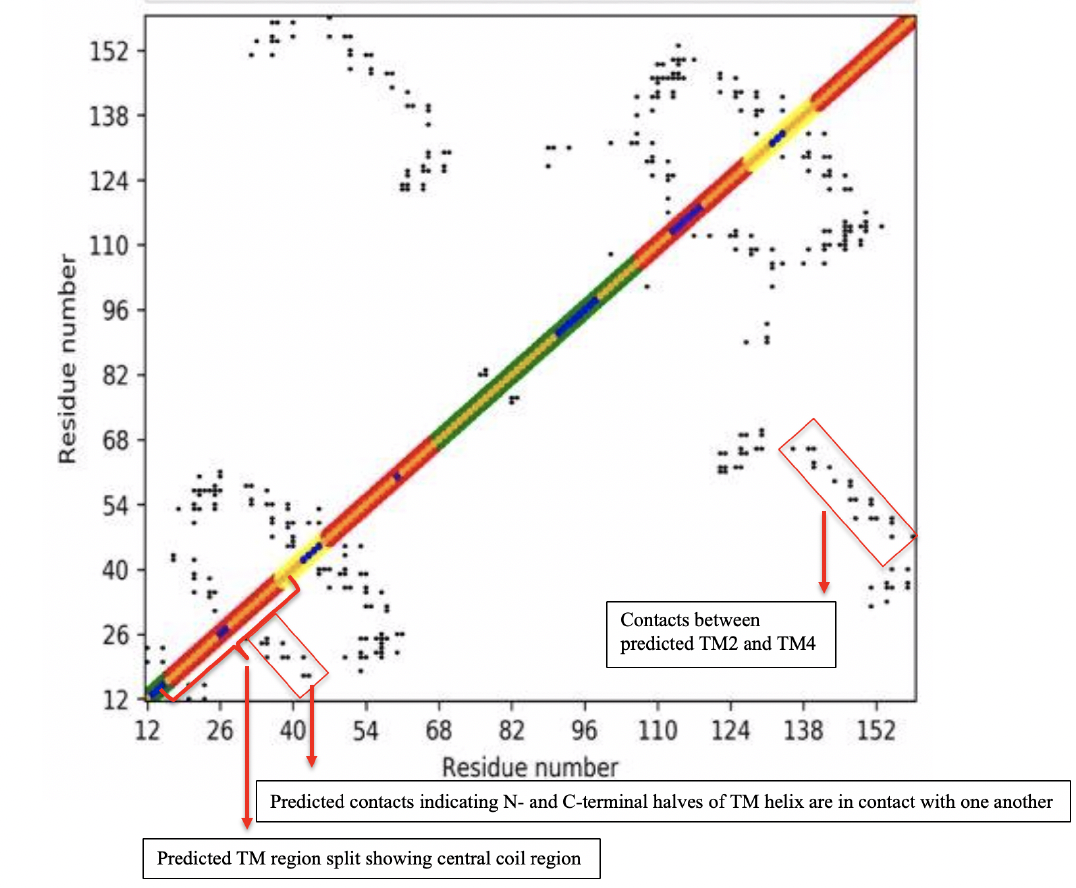
\includegraphics[width=\textwidth]{Results/enhanced_c_map_fig.png}
    \caption{Enhanced Mt2055contact map.}
    \label{fig:w9_enhan_cmap}
    \small
    Mt2055 Contact map constructed using DeepMetaPSICOV predictions with TOPCONS  membrane prediction & PSIPRED  secondary structure predictions overlaid. The outer diagonals show the TOPCONS membrane prediction (red regions being predicted TM helices, green; inside cell, yellow; outside). The thin central diagonal is the secondary structure prediction (orange, helix; blue, coil).
\end{figure}

Such a prediction would more obviously be treated as indicative of some kind of kink in the helix \cite{Law2016} but the explanation here is that these regions form re-entrant helices. A similar contact map feature can be easily generated from three transmembrane helices, however, this would result in a box feature of around 20x20 residues (and obviously reflected in the diagonal).  Since the re-entrant loop is making contact with itself this can only result in an approximately 10 residue antiparallel feature on the contact map.  Only approximately half of the transmembrane helix that is packed with the re-entrant helix will be making contact with the re-entrant loop, therefore, this would result in an additional 10 residue antiparallel feature in addition to a 10-residue parallel feature.  Together with the diagonal these will display an approximately 10x10 box feature (also reflected in the diagonal) on the contact map rather than the 20x20 box feature that three transmembrane helices (1 parallel pair and two anti-parallel ones) would produce (Figure \ref{fig:rent_cmap} ).  


\begin{figure}[th!]
    \centering
    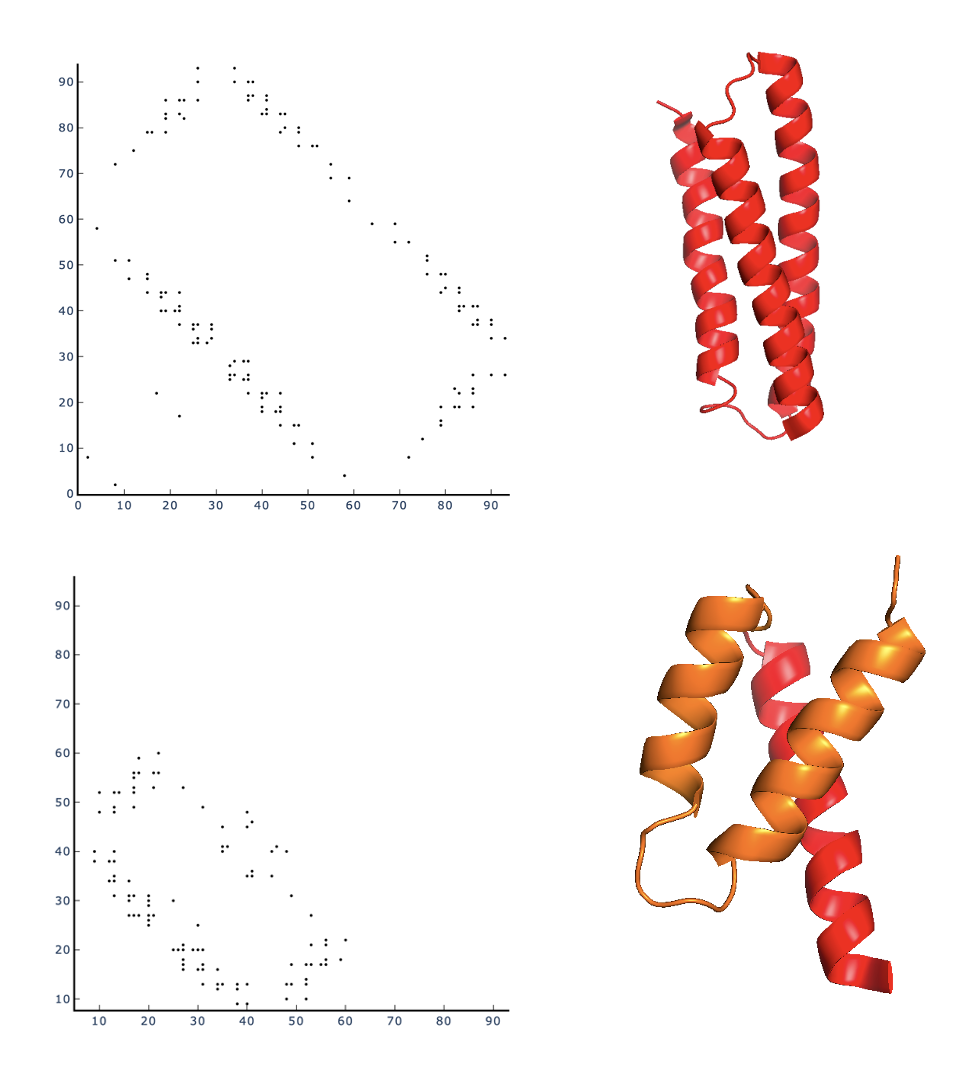
\includegraphics[width=\textwidth]{Results/rent_cmap.png}
    \caption{Re-entrant contact map.}
    \label{fig:rent_cmap}
    \small
    Top: Three transmembrane helix bundle (right) with its respective contact map (left); bottom: Re-entrant loop packed with a transmembrane helix (right) with its respective contact map (left).
\end{figure}

Similar contact map features, indicative of re-entrant loops packing against TM helices, can be seen clearly on the contact maps of other DedA proteins (data not shown). The MSA in Figure \ref{fig:msa} shows the relative positions of the re-entrant loops in their respective sequences.

Examination of the equivalent data for Tmem41b as well as the yeast homologue Tvp38 and two bacterial homologs YdjX and YdjZ revealed that all homologues contain a core consisting of an amphipathic helix, re-entrant loop and transmembrane helix in that order and inversely repeated (Figure \ref{fig:topology}). 

\begin{figure}[th!]
    \centering % <-- added
\begin{subfigure}{0.5\textwidth}
  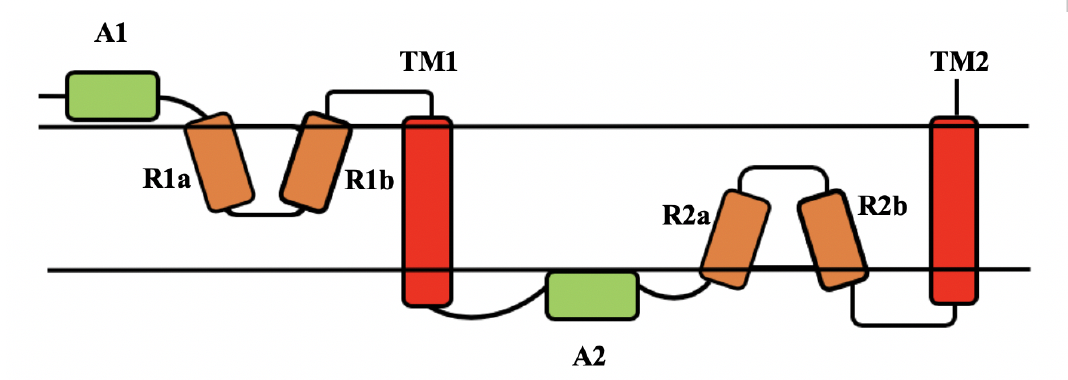
\includegraphics[width=\linewidth]{Results/w9_topology.png}
  \caption{Predicted topology for Mt2055}
  \label{fig:0}
\end{subfigure}\hfil % <-- added
\begin{subfigure}{0.5\textwidth}
  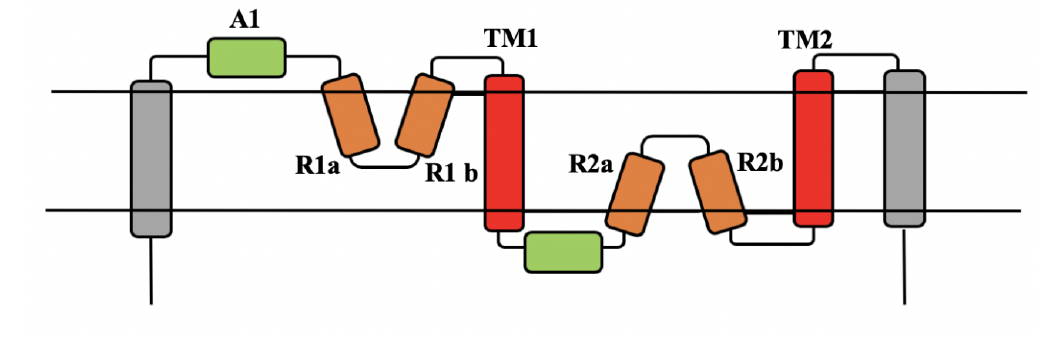
\includegraphics[width=\linewidth]{Results/tm_topology.png}
  \caption{Predicted topology for Tmem41b}
  \label{fig:1}
\end{subfigure}
\caption{DedA predicted topology}
\small
a) Predicted topology for Mt2055 based on contact, secondary structure, membrane & amphipathic predictions;
A1 – amphipathic helix 1; R1a (N-terminal half of re-entrant helix 1); R1a (C-terminal half of re-entrant helix 1; TM1- transmembrane helix 1; A2 – amphipathic helix 2; R1a (N-terminal half of re-entrant helix 2; R2a (Cterminal half of re-entrant helix 2; TM2- transmembrane helix 2.
b) Proposed topology for Tmem41b; A1 – amphipathic helix 1; R1a (N-terminal half of re-entrant helix 1; R1a (C-terminal half of re-entrant helix 1; TM1- transmembrane helix 1; A2 – amphipathic helix 2; R1a (N-terminal half of re-entrant helix 2; R2a (C-terminal half of re-entrant helix 2; TM2- transmembrane helix 2; with the presence of two-additional TM helices compared to Mt2055; Grey TM helices are additional helices to the core present in Tmem41b.
\label{fig:topology}
\end{figure}


\section{Advanced Modelling}
Alternative modelling software was identified that was not bound to membrane predictions and utilised a distance matrix approach rather than the use of the simpler quantal contact matrix restraints.  The modelling of Mt2055, Tmem41b and Yqja was executed using a locally installed version of trRosetta \cite{Yang2020} with default settings (figure  \ref{fig:trros_models}).

The Mt2055, Tmem41b and YqjA models had estimated TM scores of 0.633, 0.624 and 0.635 respectively, suggesting that they were likely to have captured the native fold of the family as a 0.5 cut off assumes generally the same fold \cite{zhang2005tm}. An all-against-all pairwise structural superposition of the models with DALI gave a mean Z-score of 11.9 confirming their strong similarity. The satisfaction of predicted contacts to validate the models (Figure \ref{fig:trros_models}) \cite{Simkovic2017} was also used to assess model quality. This showed that 80\% of the top L predicted contacts (where L is the length of the protein) were satisfied by the model contacts for both Mt2055 and YqjA and a value of 60\% was achieved for Tmem41b.  The high contact satsfaction scores are suggestive of good quality models \cite{DeOliveira2016}.  \\

Additionally, using ConPlot the superposition of the model contact map with the predicted contact map visually highlights the how close in alignment the two sets of contacts are (figure \ref{fig:w9_conplot}).\\

The models (Figure \ref{fig:trros_models}) confirmed the presence the predicted features: two inversely symmetrical repeated units each possessing a re-entrant loop (orange) packed with a TM helix (red).  In addition to this, the models also revealed that each repeating unit had a helix lying parallel to the membrane surface (green).\\

\begin{figure}[th!]
    \centering
    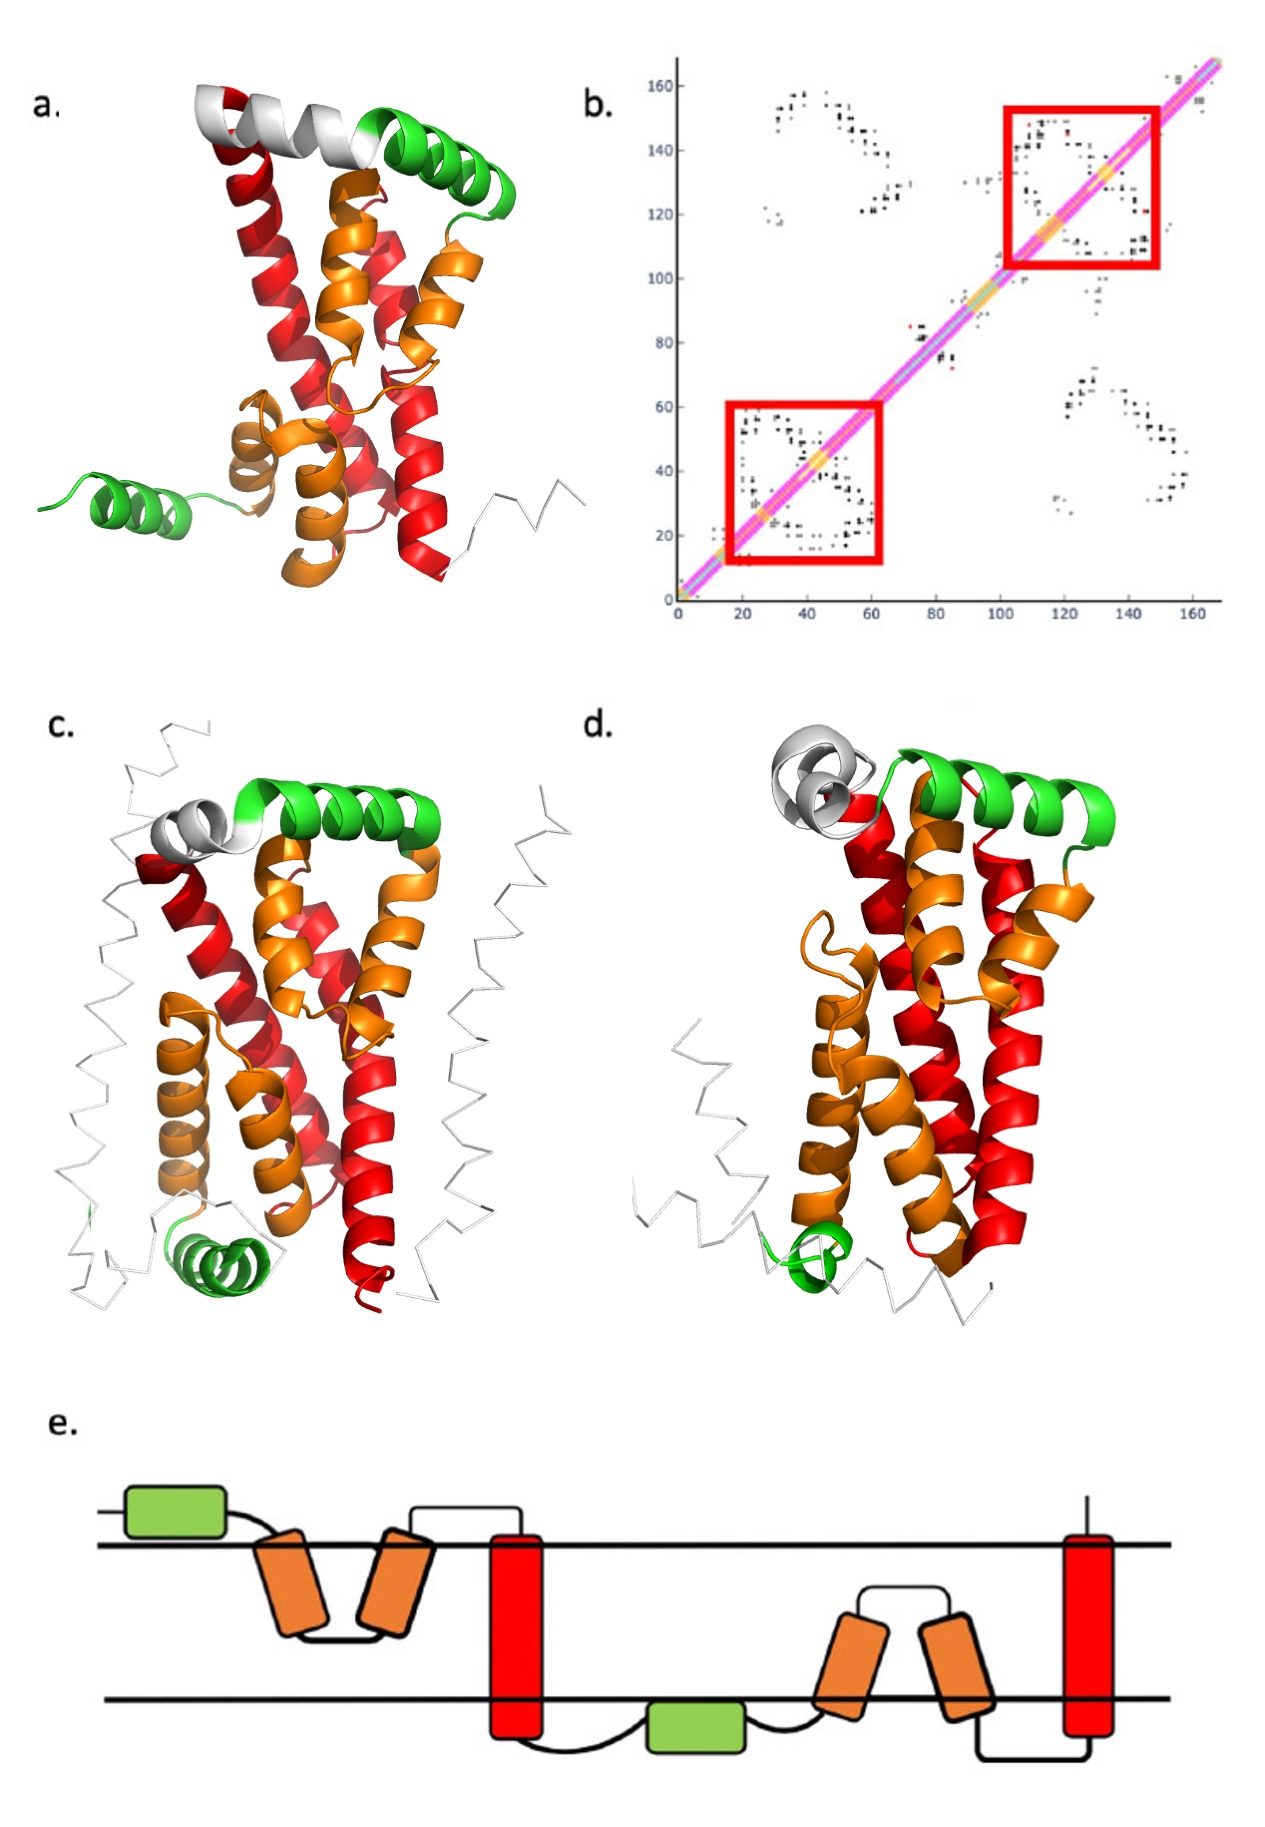
\includegraphics[width=100mm, scale =0.5]{Results/fig4.jpg}
    \caption{trRosetta Models}
    \label{fig:trros_models}
    \small
    (a) trRosetta model of MT2055 - amphipathic helix (green) and a re-entrant loop (orange) packed with a TM helix (red) (b) Superposition of DMP predicted contact map for Mt2055 and contacts from the Mt2055 model. Black points are matching contacts, red are mismatches and grey are contacts predicted but not present in the model. Diagonal is a visual representation of transmembrane helix and secondary structure prediction – central diagonal is the visualisation of the TopCons transmembrane prediction (orange being a TM helix) and the outer diagonals are the visual representation of the PSIPRED secondary structure prediction (pink – alpha helix and yellow – coil). Red boxes highlight the re-entrant loop and TM helix packing contact map signature. c) trRosetta model of Tmem41b only showing the conserved structural domain (residues 39-217) d) trRosetta model of YqjA only showing the conserved structural domain (residues 14-176). e) Proposed topology 
\end{figure}

\begin{figure}[th!]
    \centering
    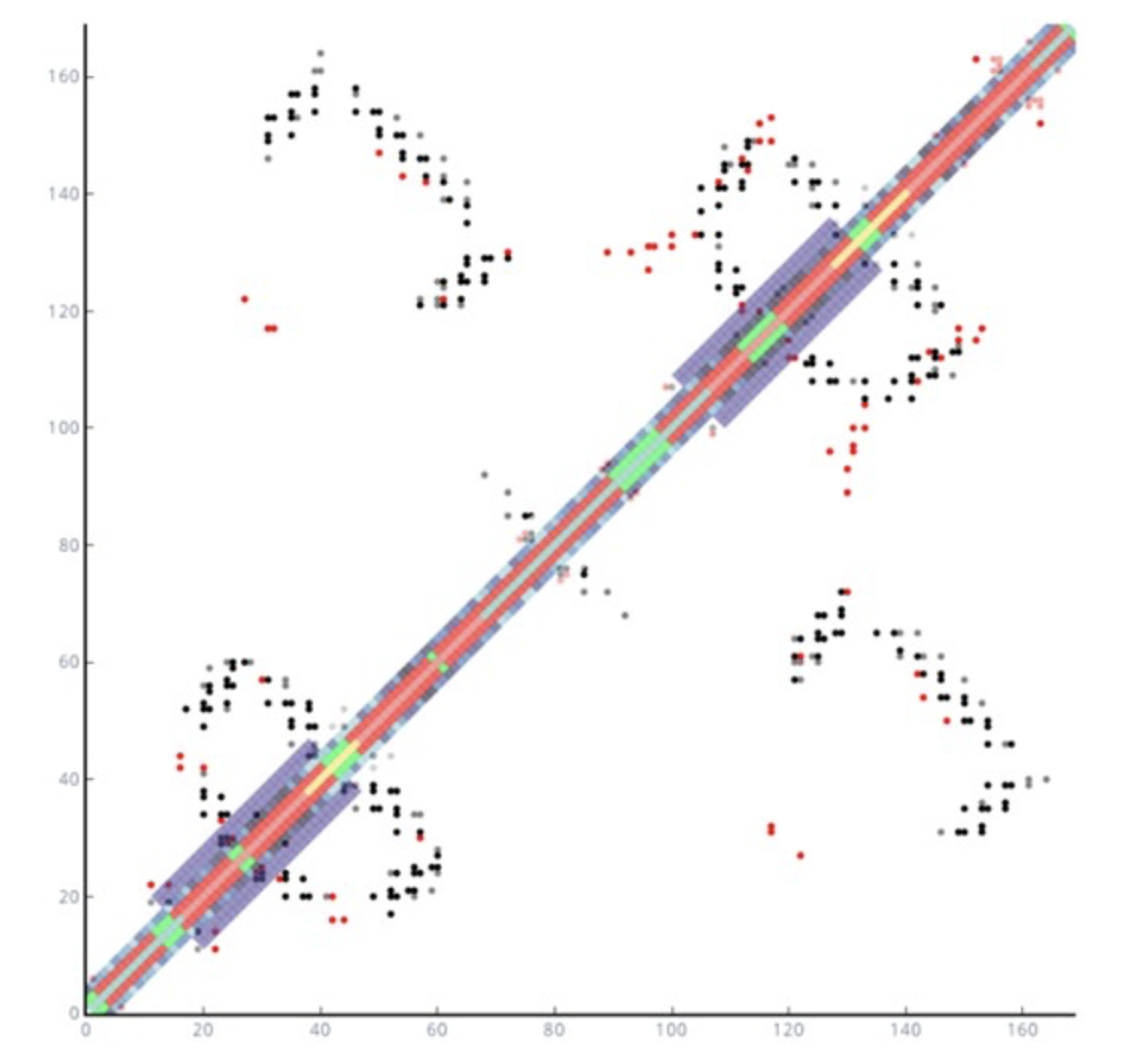
\includegraphics[width=100mm, scale =0.5]{Results/enhanced_c_map2.png}
    \caption{ConPlot Analysis}
    \label{fig:w9_conplot}
    \small
    Superposition of DeepMetaPSICOV predicted contact map with contacts present in the structure modelled with DMPfold. Black points indicate matches between the two maps, red points indicate contacts present in the model but not predicted and grey points are contacts predicted but not present in the model. Central track 0 in the diagonal is used for the TOPCONS transmembrane prediction (blue—outside cell, yellow—inside cell, light red—predicted transmembrane helix). PSIPRED secondary structure prediction is visualized by the tracks +1 and -1 adjacent to the centre of the diagonal (red—helix, green—coil). Tracks +2 and -2 represent CONSURF sequence conservation prediction (blue gradient, darker blue—more conserved, lighter blue—less conserved). Outermost tracks +3, -3, +4 and -4 were added using a custom file in which the location of the suspected re-entrant loops is highlighted in purple: between residues 16–42 and residues 105–131. 
\end{figure}


Further verification of local structures of the models was carried out. In order to test for whether the membrane-parallel helices (green in Figure \ref{fig:trros_models}) were amphipathic, an analysis of helical wheel diagrams for the fifteen residues preceding the putative re-entrant loops was performed with HELIQUEST \cite{Gautier2008}. The quantitative measures of the hydrophobic moment for the regions being analysed (Figure \ref{fig:heliquest}) support that they are indeed amphipathic helices. The hydrophobic moments ranged from 0.298 to 0.546 on a scale of 0-1.

\begin{figure}[th!]
    \centering
    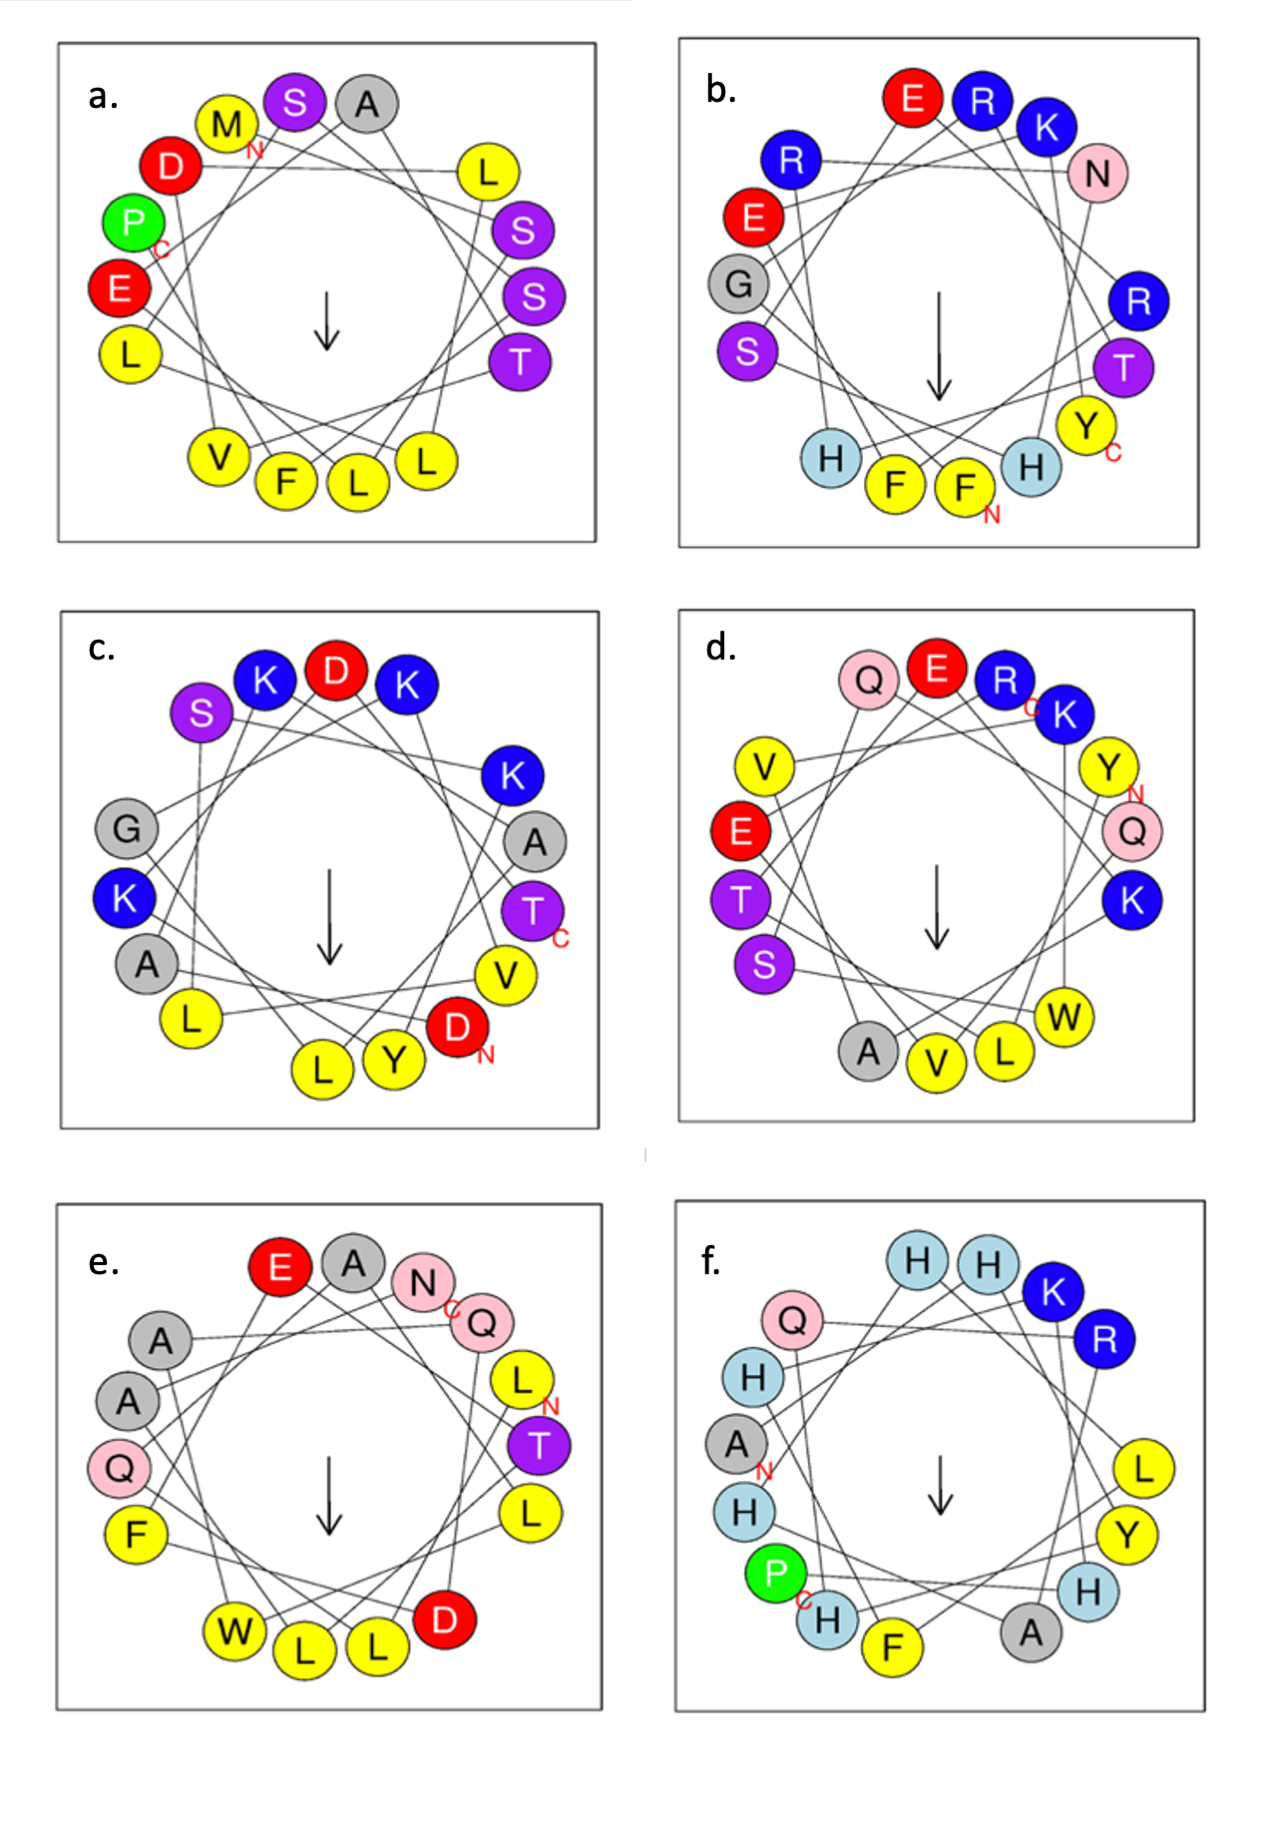
\includegraphics[width=125mm, scale =0.5]{Results/fig5.png}
    \caption{Helical wheel diagrams generated using the HELIQUEST server}
    \label{fig:heliquest}
    \small
    Hydrophobic residues are shown in yellow, serine and threonine in purple, basic residues in dark blue, acidic residues in red, asparagine and glutamine in pink, alanine and glycine in grey, histidine in light blue and proline in green circles. Arrows represent direction and magnitude of the hydrophobic moment and residue marked with ‘N’ is the N-terminal end of the putative amphipathic helix with the residue marked ‘C’ being the C-terminal end. (a) Mt2055 putative amphipathic helix 1 (hydrophobic moment of 0.298). (b) Mt2055 putative amphipathic helix 2 (hydrophobic moment of 0.546). (c) Tmem41b putative amphipathic helix 1 (hydrophobic moment of 0.471). (d) Tmem41b putative amphipathic helix 2 (hydrophobic moment of 0.420). (e). YqjA putative amphipathic helix 1 (hydrophobic moment of 0.295). (f) YqjA putative amphipathic helix 2 (hydrophobic moment of 0.396).
\end{figure}

The predicted presence of the amphipathic-re-entrant loop-TM helix features in DedA domain proteins prompted a desire to map sequence conservation on to the ab initio models. Using the CONSURF server to perform the mapping of sequence conservation onto the query models, it revealed that the re-entrant loop sequences are highly conserved. The high sequence conservation of re-entrant loops indicate that they are likely to be functionally and/or structurally important (Figure \ref{fig:consurf}).

\begin{figure}[th!]
    \centering
    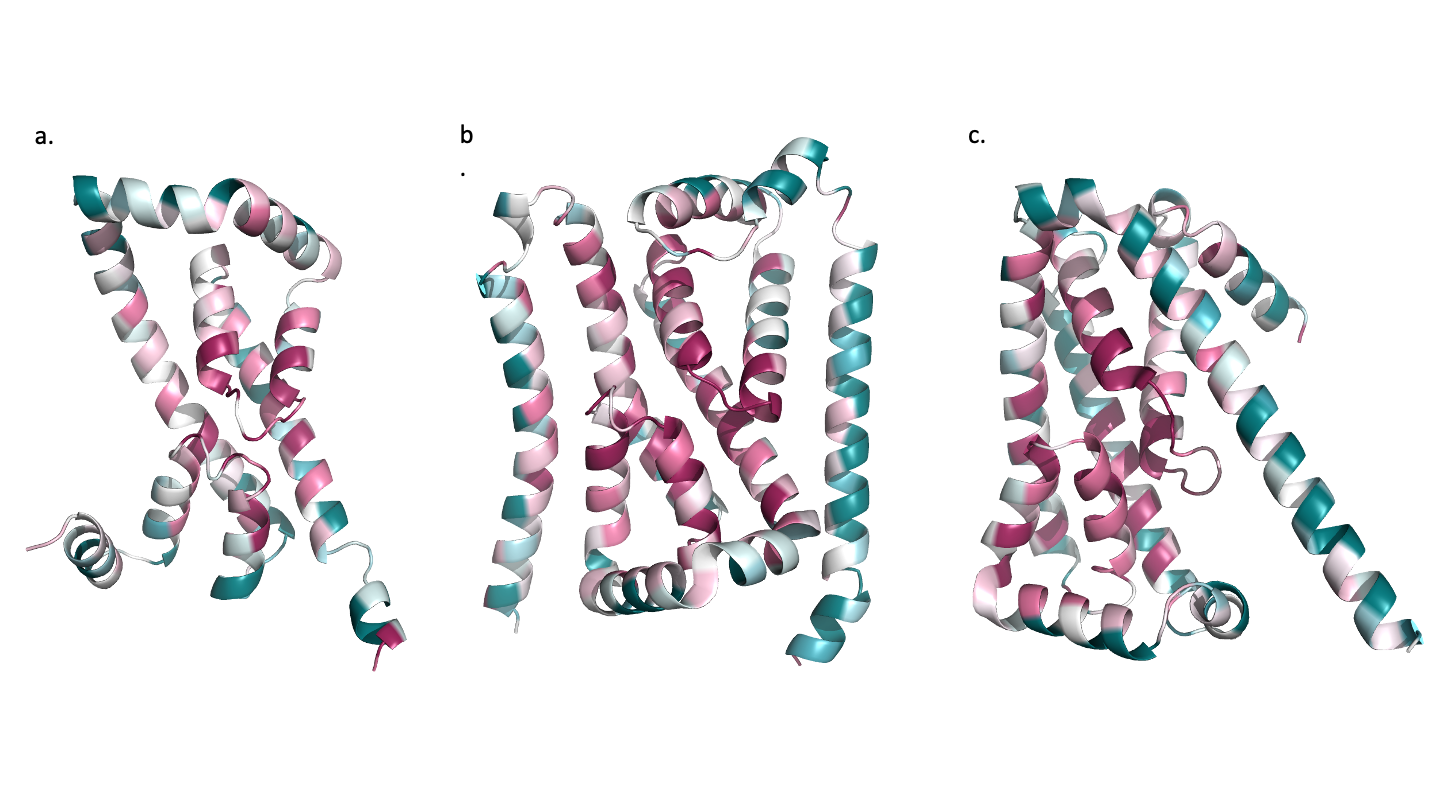
\includegraphics[width=\textwidth]{Results/fig6.png}
    \caption{CONSURF conservation mapping}
    \label{fig:consurf}
    \small
    trRosetta models with Consurf conservation mapping for (a) Mt2055 (b) Tmem41b (c) YqjA. Conservation is shown as a spectrum from purple (highly conserved) to blue (not conserved).
\end{figure}


Re-entrant loops were initially reported in the early 1990s in the cardiac Na\textsuperscript{+}/Ca\textsuperscript{2+} exchanger \cite{iwamoto1999unique}.
Since then re-rentrant loops have been detected in other membrane transporters and channels such as aquaporins \cite{de2001refined}, potassium channels \cite{zhou2001chemistry} and chloride channels \cite{dutzler2002x}.  The sequence-structure relationships of re-entrant loops have been studied before \cite{Yan2010} revealing that while TM helices have an even distribution of hydrophobic residues, re-entrant loops show an uneven distribution. Indeed, examination of the putative re-entrant loop sequences identified an inconsistent hydrophobicity distribution in both putative re-entrant loops of the homologues studied here (Figure \ref{fig:hydro_profiles}) with the C-terminal side being more hydrophilic. Interestingly it is the residues around the turning points of the re-entrant loops that more conserved (Figure \ref{fig:consurf}).  

\begin{figure}[th!]
    \centering
    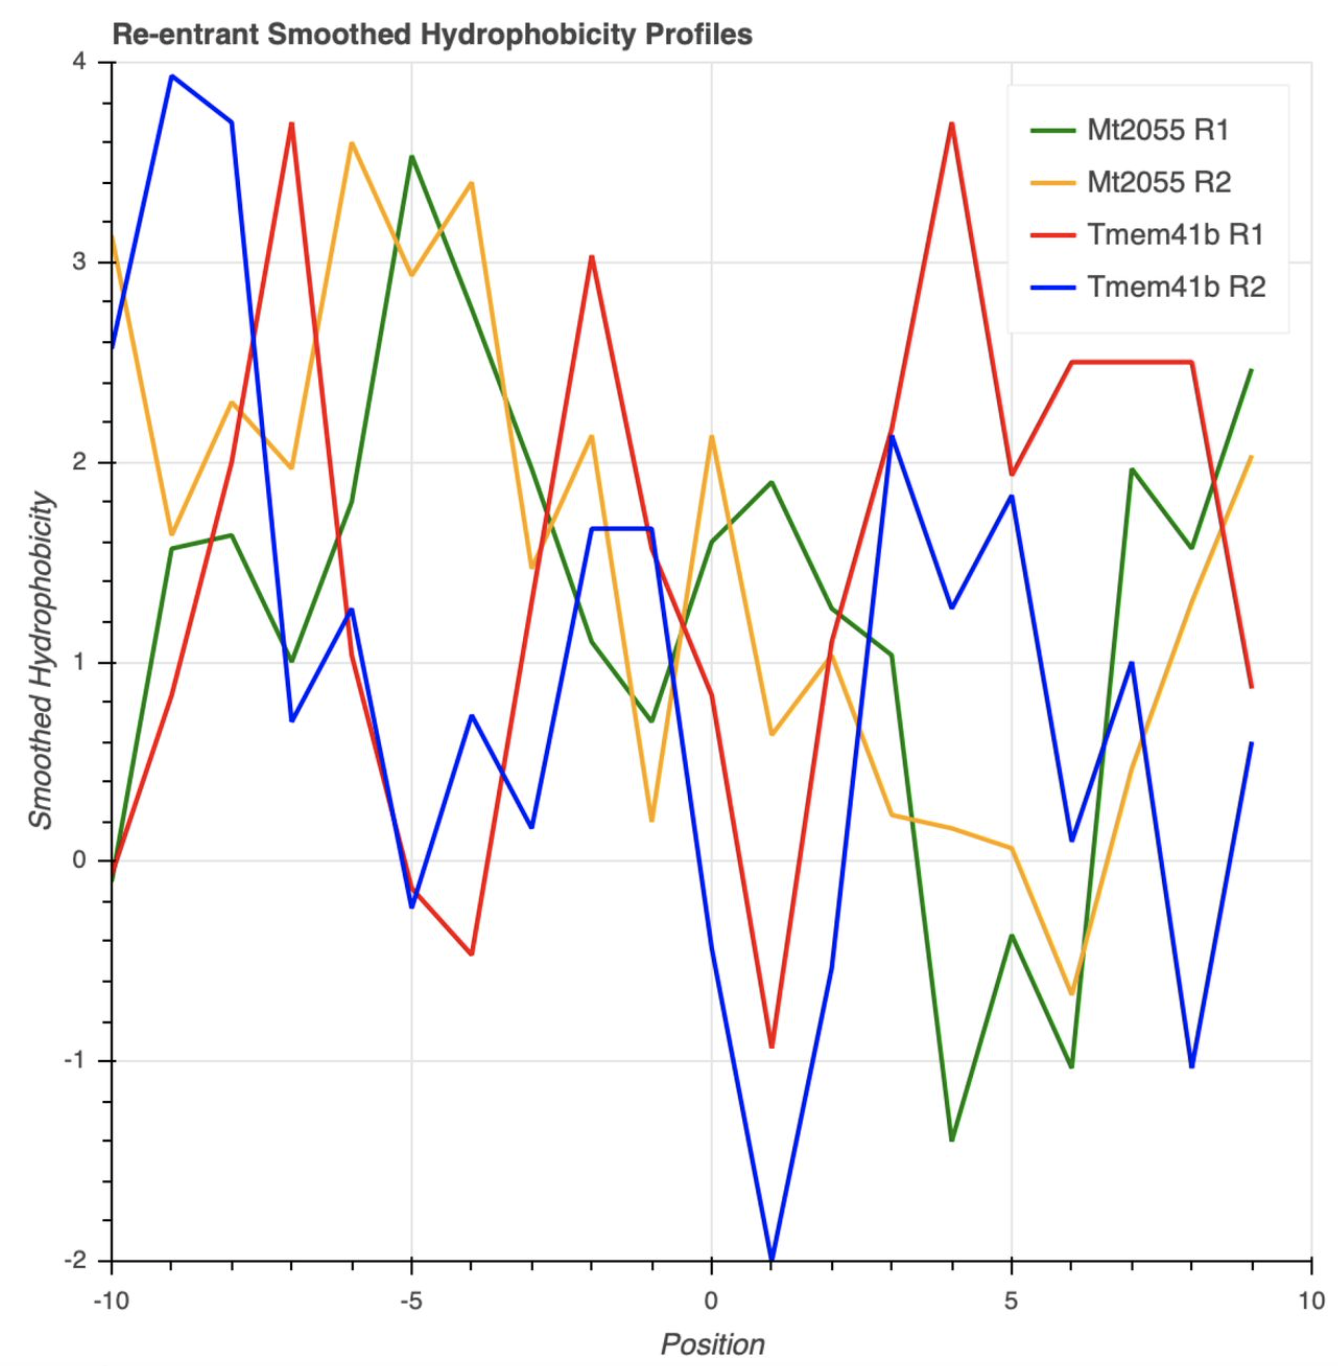
\includegraphics[width=125mm, scale =0.5]{Results/hydro_profiles.png}
    \caption{Re-entrant hydrophobic profiles}
    \label{fig:hydro_profiles}
    \small
    Smoothed hydrophobicity profiles for putative re-entrant loops of Mt2055 and Tmem41b. Smoothed the hydrophobicity distribution using a sliding window of three residues. For each position the mean hydrophobicity \cite{Kyte1982} of the three positions covered by the window is calculated and assigned to the position at the center of the window. Positions are numbered by assigning the central residue (proline; see later) as 0.
\end{figure}

Assessing the conservation across the sequence of PF09335/PF06695 homologues, ConSurf highlights regions of strong conservation. The strongly conserved regions are located in at the turning points of the re-entrant loops  and the mid-points of the tranmembrane helices that are packed against the re-entrant loops.  These regions come together in three-dimensional space. \\

In an effort to locate the presence of any functional residues the CONSURF data at the regions of highest conservation were examined. As expected from the sequence analysis, the conservation data identified the presence of proline residues at the ‘turning point’ of all putative re-entrant loops in the MSAs. Thus, the conserved proline identified above is suggested by the models to have a structural role providing the tight turn required for the approximate 20° (figure \ref{fig:angles}) angle making up the re-entrant loop.  


\begin{figure}[th!]
    \centering
    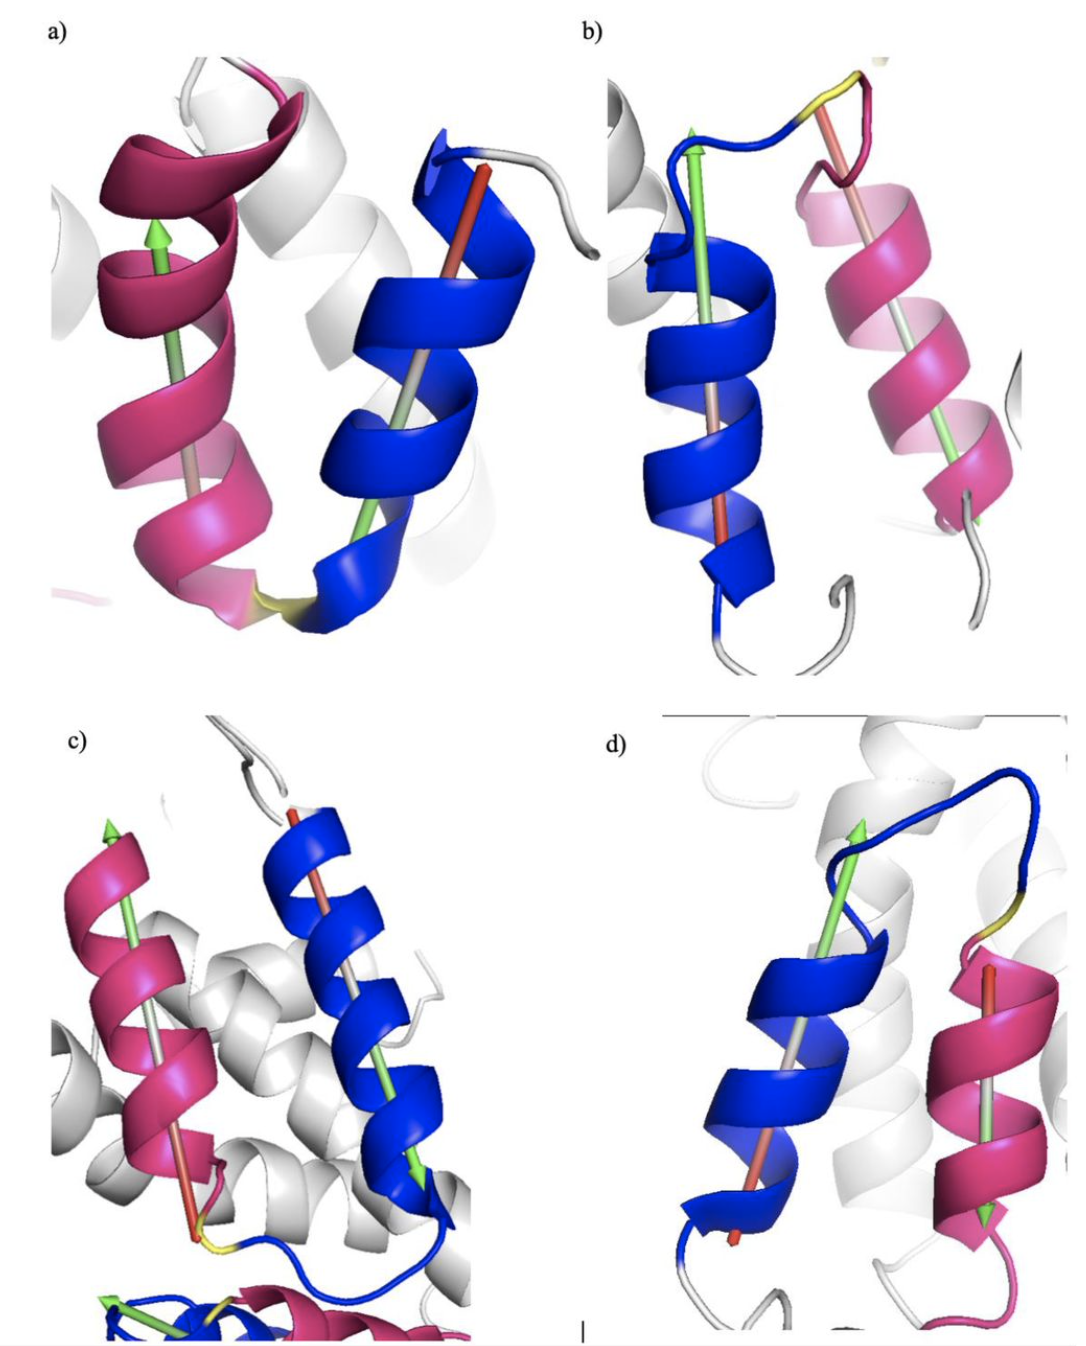
\includegraphics[width=125mm, scale =0.5]{Results/re_angles.png}
    \caption{Re-entrant angle measurements}
    \label{fig:angles}
    \small
    Tight re-entrant turn of around 160° a) Mt2055 R1 b) Mt2055 R2 c) Tmem41b R1 d) Tmem41b R2. Blue is C-terminal side of re-entrant loop, pink is N-terminal side of re-entrant loop, yellow is position of the proline. It can be seen that the proline residue is slightly off set from the turning point in some re-entrant loops possibly as a result of inaccuracy in the modelling.
\end{figure}

\section{Clustering of re-entrant loops}
The presence of re-entrant loops and the high density of conserved residues within them prompted an examination of experimentally characterised re-entrant loops in the PDBTM database. A total of 56 non-redundant re-entrant helices were identified (see Methods). All 56 were clustered with the putative re-entrant loops from Mt2055 and four PF09335 homologues (Tmem41b, Tvp38, YdjX and YdjZ) using relative E-values derived from an all-against-all BLAST run in CLANS \cite{Frickey2004} with a 0.1 p-value cut-off. The largest cluster contained 14 sequences, of which four were putative re-entrant sequences from the query proteins (Mt2055 C-terminal re-entrant, YdjX C-terminal re-entrant, Ydjz N-terminal re-entrant and YdjZ C-terminal re-entrant), seven (3org, 5tqq, 3nd0, 3det and 6coy) were re-entrant loop sequences from Cl\textsuperscript{-}/H\textsuperscript{+} antiporters, one was from a boron exchanger (5l25), one from an electron transporter (2n4x) [albeit classified as a member of the lysine exporter superfamily \cite{Saier2016}] and one from a mechanogated channel (5z10).\\

Analysis of the Cl\textsuperscript{-}/H\textsuperscript{+} antiporter structures show that they contain a similar inverted repeat as we infer for the DedA homologues, resulting in pseudo-2-fold axis of symmetry running along the membrane \cite{Duran2013}. Again similarly, the Cl\textsuperscript{-}/H\textsuperscript{+} antiporter 3orgA also contains the amphipathic helices on the N-terminal side of the re-entrant loops. The fact that the presence of the amphipathic helices is restricted only to 3orgA and not found in all homologues suggest that these features are not essential for function. A similar distribution of conservation is observed between the putative pore region of Tmem41b and the Cl\textsuperscript{-}/H\textsuperscript{+} antiporter 3orgA (Figure \ref{fig:3org}(d)). Analysing the sequence of all re-entrant loops of the top cluster (comprising members of the Tmem41b family and the transporters) revealed that they all contain a proline at the turning-point. \\

 
 
 A second clustering exercise was implemented where all re-entrant loops in addition to the proceeding 30 residues were extracted from a non-redundant re-entrant loop containing subset of the PDB. The resulting 193 library entries, supplemented with the re-entrant loop features from the ab initio models, underwent an all-against-all structural alignment utilising Dali. The Z-scores for these alignments were then used to cluster all the structures.  This screen resulted in the Mt2055, Tmem41b and YqjA re-entrant loop feature structures clustering with the re-entrant loop features of Cl\textsuperscript{-}/H\textsuperscript{+} antiporters; this was a similar result to the original sequence-based clustering; as expected all six re-entrant structures from the query models clustered together. The CLC transporter re-entrant structures of 3orgA (re-entrant 1 and re-entrant 2), 7bxu and 5tqq also clustered with the queries. Additionally, the re-entrant structure from an Undecaprenyl pyrophosphate phosphatase (UppP) (6cb2) also clustered with the queries. UppP is an integral membrane protein that recycles lipid and has structural similarities to CLC transporters \cite{Workman2018}. Contact maps derived from the pdb files of CLC and UppP structures show the contact map signature corresponding to the re-entrant/TM helix structural feature (data not shown). Interestingly, the UppP is more similar to the PF09335 family being only 271 residues in length and having only 6 TM helices with UppP being involved in phospholipid trafficking; a function possibly related to autophagosome construction which Tmem41b has been shown to be involved with. 
 \begin{figure}[th!]
    \centering
    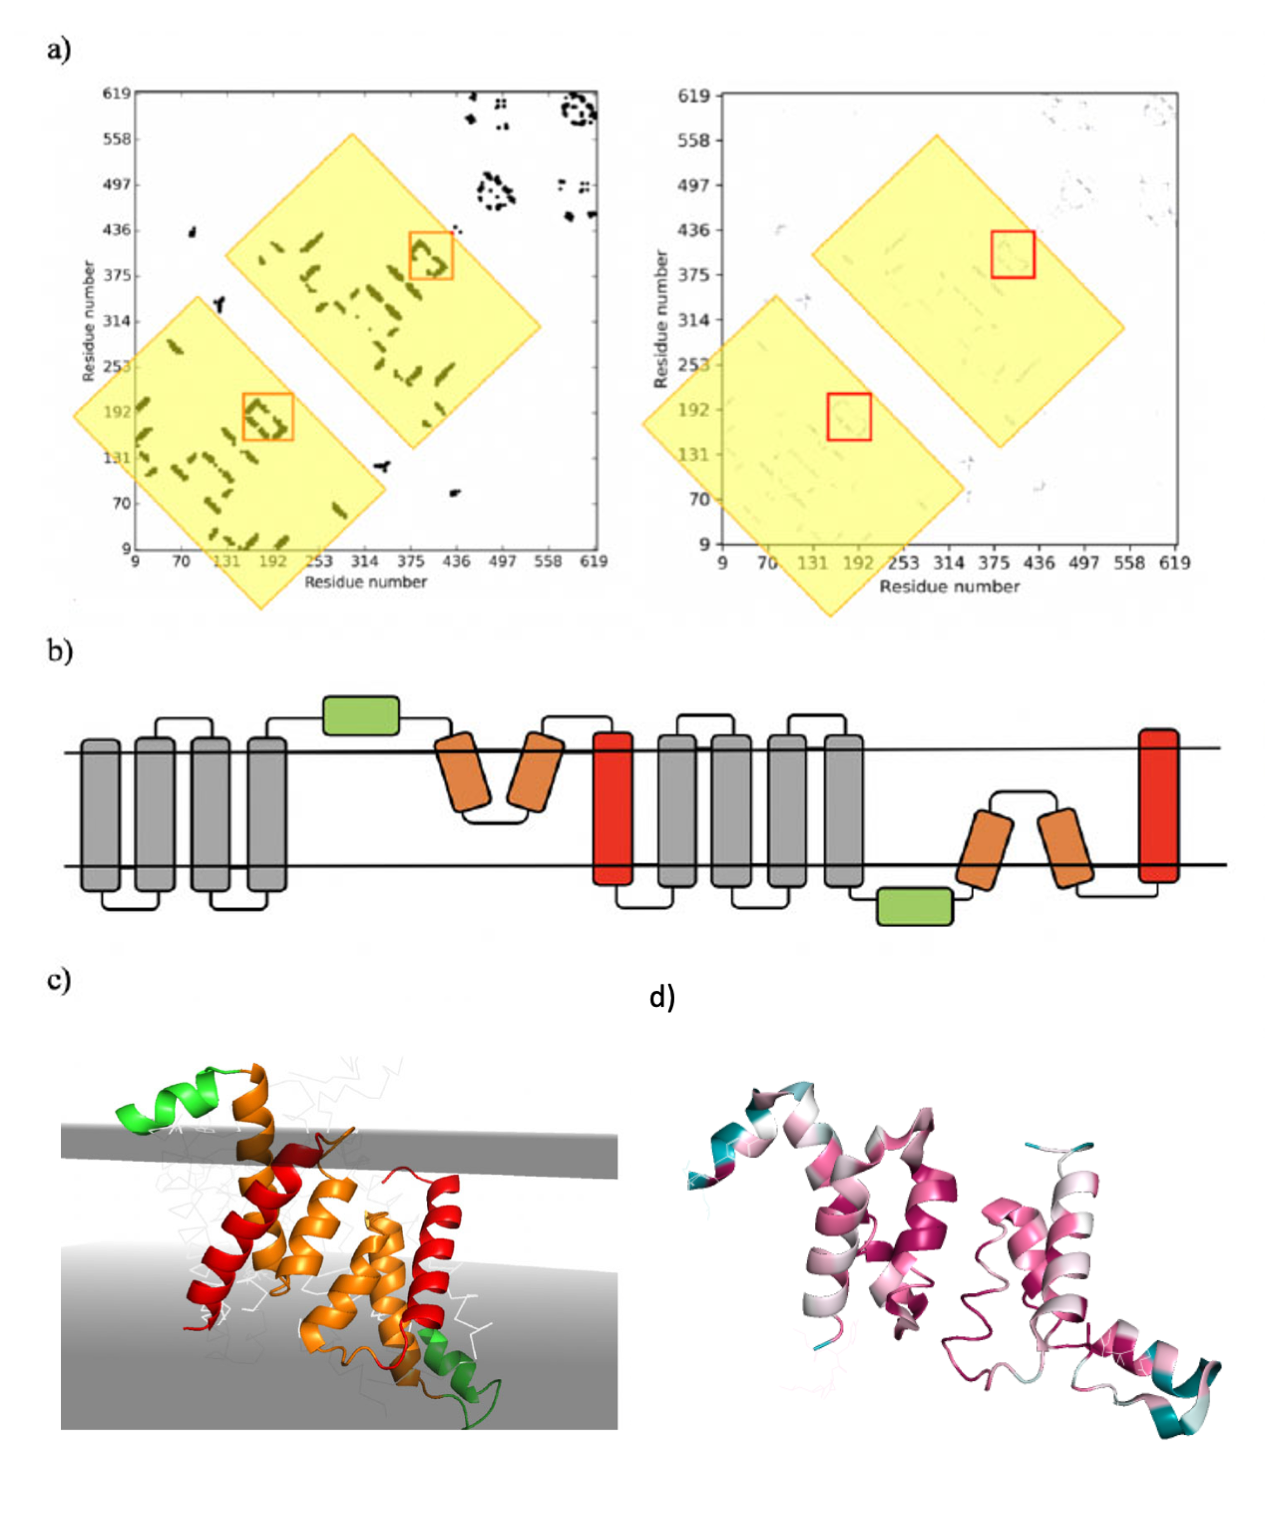
\includegraphics[width=150mm, scale =0.75]{Results/fig7.png}
    \caption{3orgA Analysis}
    \label{fig:3org}
    \small
    (a) Left - Predicted Contact map with repeating units highlighted in yellow boxes, contact map signature of re-entrant loop packed with TM helix in red boxes.; Right - The Experimental Contact map obtained from the PDB structure with repeating units highlighted in yellow boxes, contact map signature of re-entrant loop packed with TM helix in red boxes. (b) Actual 3orgA topology; grey: TM Helices that are additional to the core; red: TM helices contributing to the formation of the core; orange; re-entrant loops contributing to the formation of the core; green: amphipathic helices contributing to the formation of the core. (c) The 2-fold pseudo symmetry of the amphipathic/re-entrant loop/TM helix core inverted repeat structure of 3orgA with membrane positions shown as grey planes obtained from PDBTM.(d) Consurf conservation mapping on to the core inverted repeat structure of 3orgA.
\end{figure}

 In order to test whether 6cb2 predictions would generate the same contact map features as PF09335 and PF06695 homologues,  a TopCons \cite{Tsirigos2015} topology prediction was used to compare the predicted membrane topology of 6cb2 to its actual topology.  This exercise resulted in TopCons predicting false positive transmembrane helices at the positions of the re-entrant loops, as what was proposed for Tmem41b and homologues.  To investigate further, visual representations of the membrane topology from TopCons and the PSIPRED secondary structure prediction were plotted along the diagonal of the contact prediction for 6cb2 (Figure \ref{fig:6cb2_conplot}).  This clearly highlights that the N- and C- halves of the TopCons false positive predicted transmembrane helices in question were making contact with each other (by a length of around 10 residues).  Additionally, the secondary structure plot shows an interruption at the halfway point of the predicted transmembrane helices which would account for the abrupt change in direction of helix in the membrane.
 \begin{figure}[th!]
    \centering
    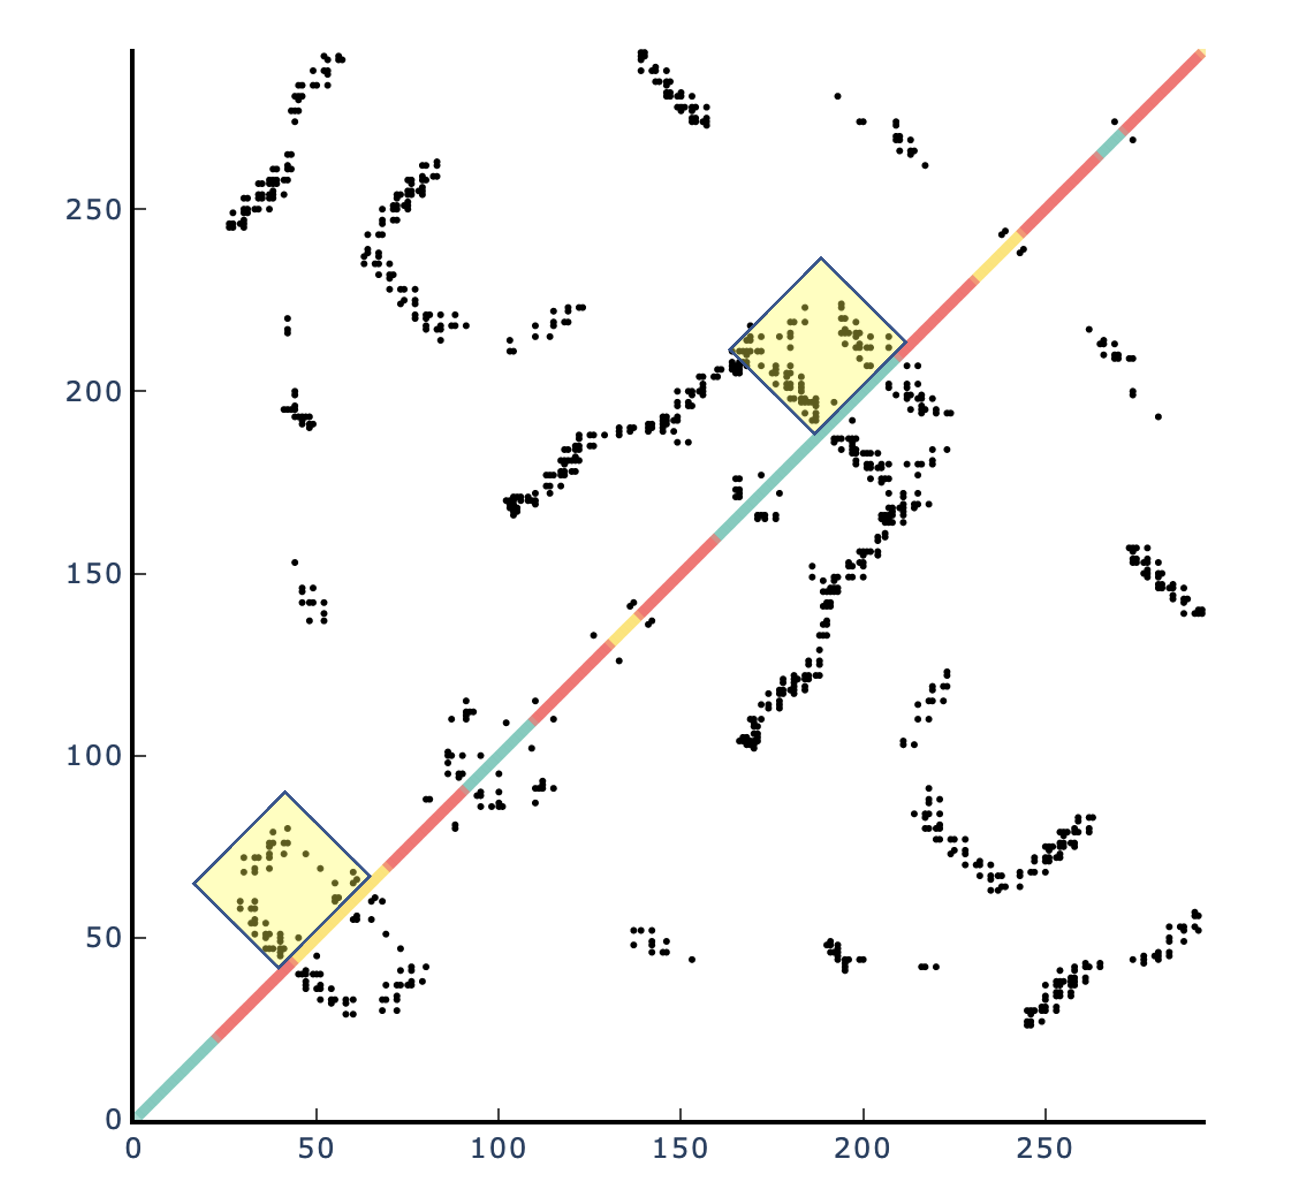
\includegraphics[width=\textwidth]{Results/6cb2_c_map.png}
    \caption{6cb2 Contact map}
    \label{fig:6cb2_conplot}
    \small
    Contacts for 6cb2 (black points) and a visual representation of the TopCons topology prediction (green -outside, red – TM helix, yellow-inside, yellow boxes are the re-entrant loop-TM-helix ‘signature’).  Cross-referencing the first re-entrant contact map  feature with the TopCons topology prediction it is clear that the TopCons topology must be wrong; the first TopCons predicted TM helix cannot be making contact with a region out-side of the membrane.  Indeed, examination of the crystal structure reveals that the contact feature highlighted does in fact result from a re-entrant loop packed with a TMhelix .
\end{figure}

A recent study has identified key residues (Figure \ref{fig:Yqja}) in the E. coli DedA protein YqjA that, when replaced in site directed mutagenesis experiments, resulted in properly folded (membrane localized) but non-functional proteins unable to complement alkaline pH sensitivity of E. coli YqjA mutant and antibiotic sensitivity of YqjA/YghB double mutant \cite{Panta2019}. Highlighting the essential residues (E39, D51, R130 and R136) on the YqjA model is striking as they come together in three-dimensional space with the N-terminal side of the first re-entrant possessing E39 and the C-terminal side possessing D51. R130 and R136 are similarly positioned on the second re-entrant loop (Figure \ref{fig:Yqja}). Re-entrant loops are known to form pores and here we have two proton-titratable residues (E39, D51) in close proximity to essential basic residues (R130 and R136) within a putative pore. This three-dimensional arrangement of key residues could serve a role in the coupling of the protonation status with the binding of a yet to be characterised substrate as is postulated for the multi-drug H\textsuperscript{+} antiporter MdfA \cite{Heng2015} where these same residues are located inside a central cavity.  

\begin{figure}[th!]
    \centering
    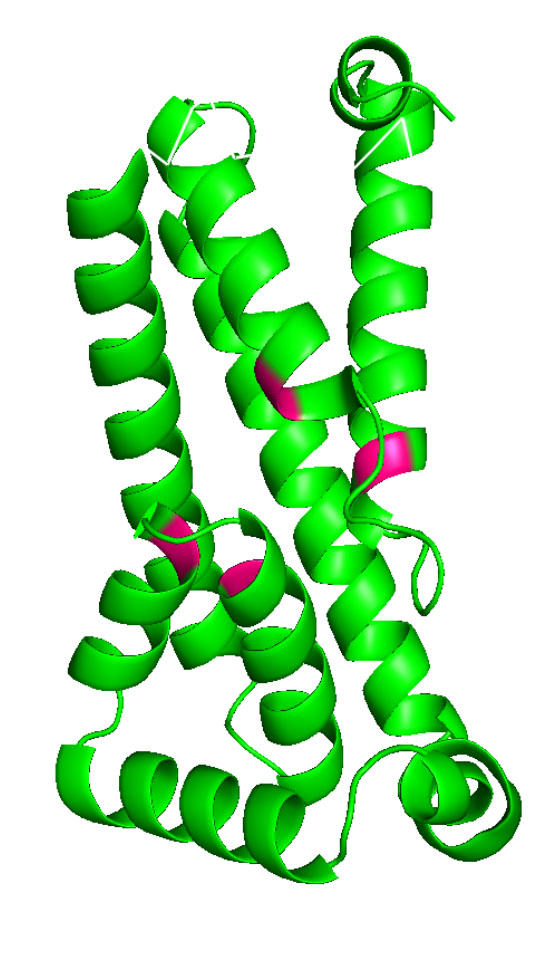
\includegraphics[width=50mm, scale =0.5]{Results/fig8.jpg}
    \caption{Annotated Yqja model}
    \label{fig:Yqja}
    \small
    Essential residues determined by SDM experiments highlighted in pink on a truncated YqjA model
\end{figure}

\section{Model Stability}
As it can be seen on Figure \ref{fig:3org}(c) that 3org contains additional helices that surround the interfacial helix - re-entrant loop - transmembrane motif. Indeed 3org forms a dimer, where the dimer interfaces are formed by the re-entrant loops and the additional transmembrane helices that surround this core. This arrangement ensure the lipid embedded structure is energetically stable \cite{Feng2010}. In the proposed model for the PF09335 and PF06695 homologues, the re-entrant loops are not wrapped by other helices thus lipids may interact them; this could be energetically unfavorable.  However, the shielding of the re-entrant loops produced by this wrapping could be achieved in Tmem41b and other family members by a similar dimerization as seen in 3org. Indeed, homodimers and higher oligomers have been detected experimentally in \emph{E. coli} YqjA \cite{Keller2015, scarsbrook2021topological}. Furthermore, submission of all three of the final models to the DeepHomo server \cite{yan2021accurate} reveals the clustering of moderately strong contact predictions (with a reliability > 0.5) that are not satisfied by the 3D monomeric structure and hence are consistent with homomeric intermolecular interactions being conserved across the family (figure \ref{fig:deephomo}). 

\begin{figure}[htb]
    \centering % <-- added
\begin{subfigure}{0.5\textwidth}
  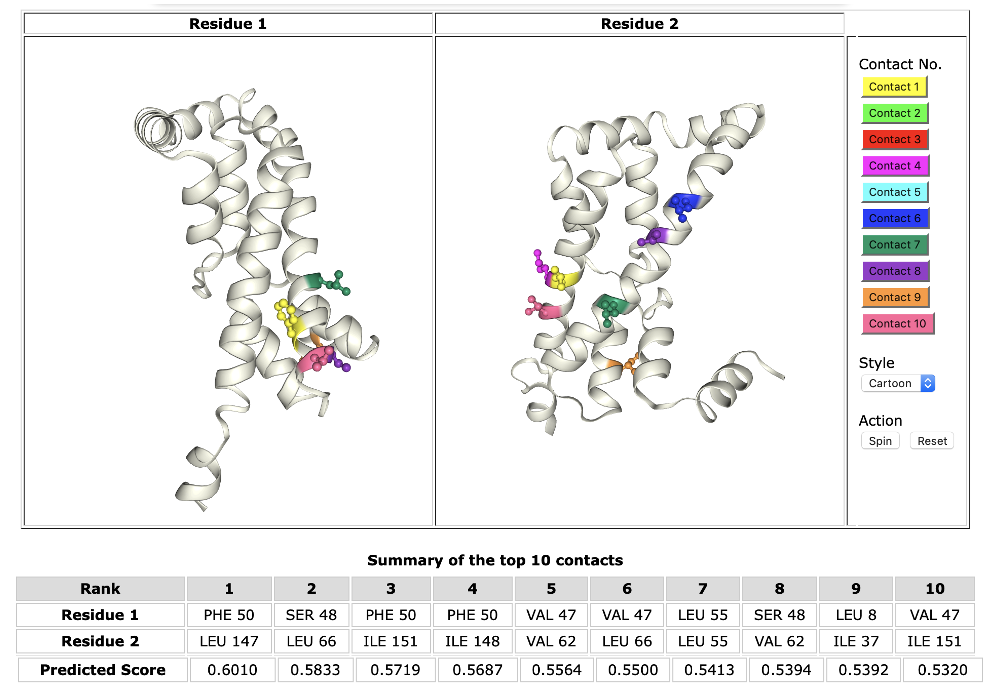
\includegraphics[width=\linewidth]{Results/w9_deep_homo.png}
  \caption{DeepHomo results for Mt2055}
  \label{fig:0}
\end{subfigure}\hfil % <-- added
\begin{subfigure}{0.5\textwidth}
  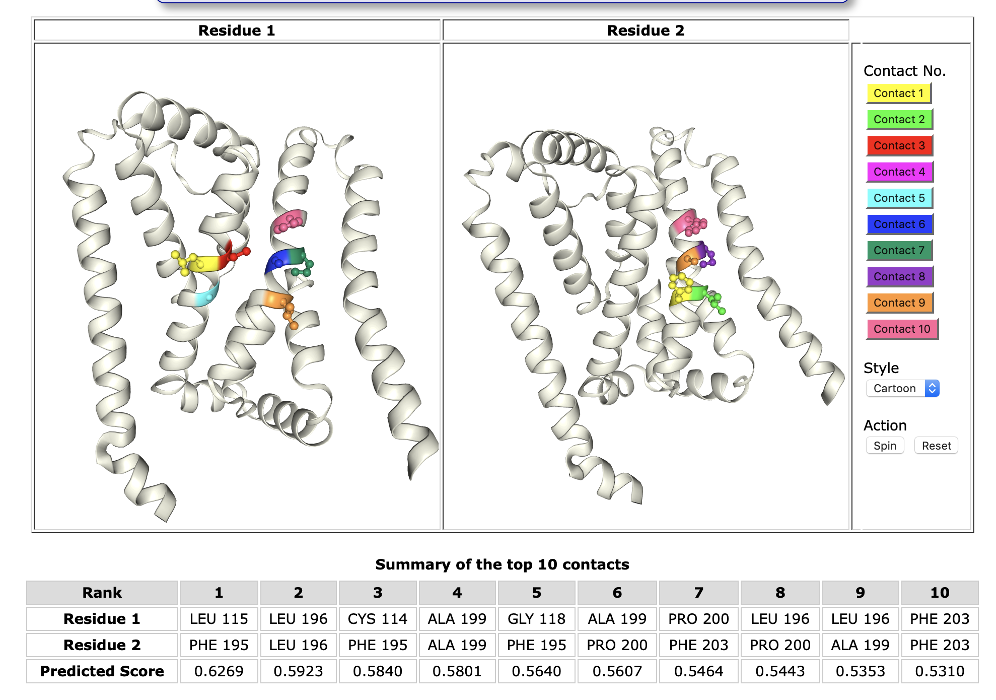
\includegraphics[width=\linewidth]{Results/tm_deephomo.png}
  \caption{DeepHomo results for Tmem41b}
  \label{fig:1}
\end{subfigure}
\caption{DeepHomo Results}
\small
The figure depicts two identical monomers displayed side-by-side, highlighting two corresponding residues involved in a contact. Summary of rankings and residue pairs for the top 10 contacts are displayed. The predicted scores range from 0.0 to 1.0, where higher scores indicate a higher likelihood of contact between the residue pairs.
\label{fig:deephomo}
\end{figure}

\section{AlphaFold2 Modelling}
The recent release of AlphaFold2 (AF2) \cite{Jumper2021} provided another opportunity to model Tmem41b and related proteins.  AF2 constructed models that support the trRosetta monomer predictions (Figure \ref{fig:w9_af}); aligning each of the trRossetta models for Mt2055, Tmem41b and YqjA with their respective AF2 counterparts yielded Z-scores of 18.4, 21 and 19.4 respectively.  Figure \ref{fig:af2_modelling} provides a visual insight of how the DedA domain modeling evolved during the period of this PhD; displaying the output models from the three incarnations of Rosetta to an AF2 model. 

Attempts to model homodimers of Mt2055 utilising the multimer mode of AF2 proved unsuccessful; chains of the output models did not come together to form an interface.  


\begin{figure}[htb]
    \centering % <-- added
\begin{subfigure}{0.25\textwidth}
  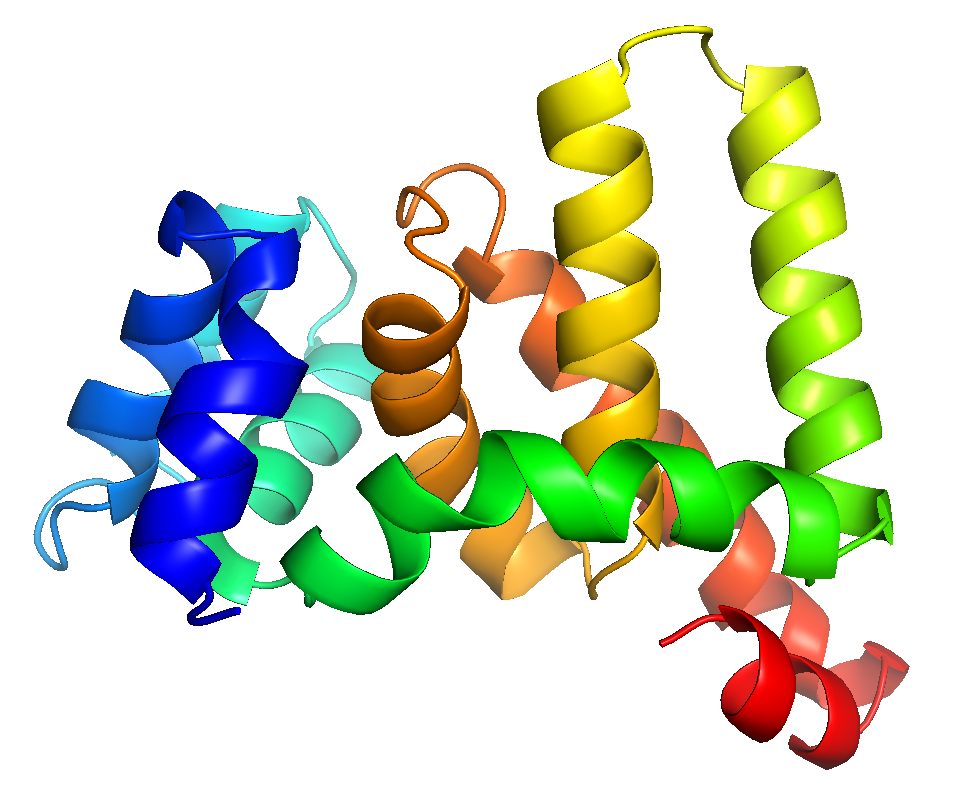
\includegraphics[width=\linewidth]{Results/w9_ros.png}
  \caption{Rosetta ab initio Mt2055 model}
  \label{fig:w9_ros}
\end{subfigure}\hfil % <-- added
\begin{subfigure}{0.25\textwidth}
  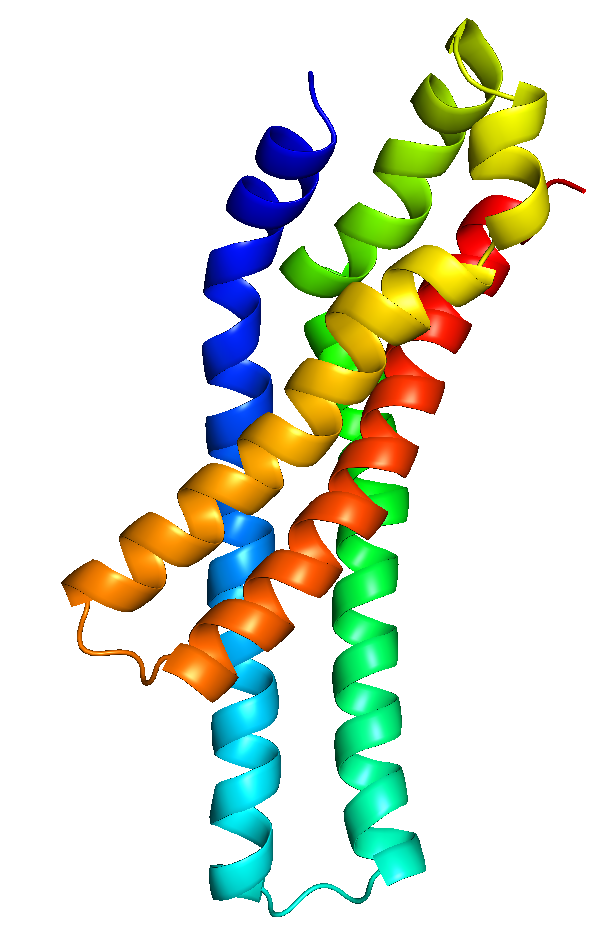
\includegraphics[width=\linewidth]{Results/w9_rosM.png}
  \caption{RosettaMembrane Mt2055 model}
  \label{fig:w9_rosM}
\end{subfigure}
\begin{subfigure}{0.25\textwidth}
  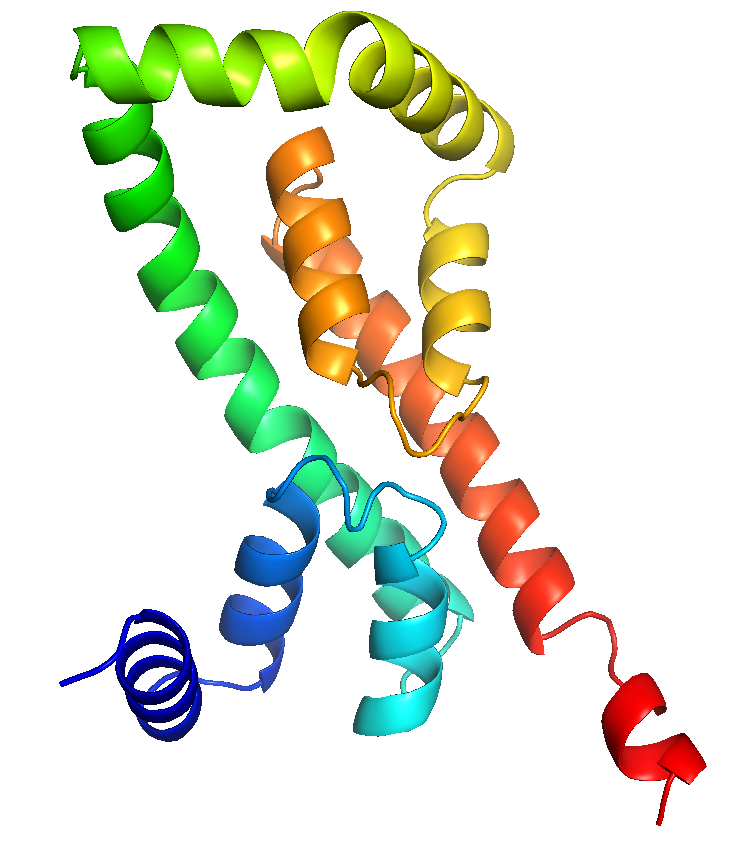
\includegraphics[width=\linewidth]{Results/w9_tr.png}
  \caption{trRosetta Mt2055 model}
  \label{fig:w9_tr}
\end{subfigure}\hfil % <-- added
\begin{subfigure}{0.25\textwidth}
  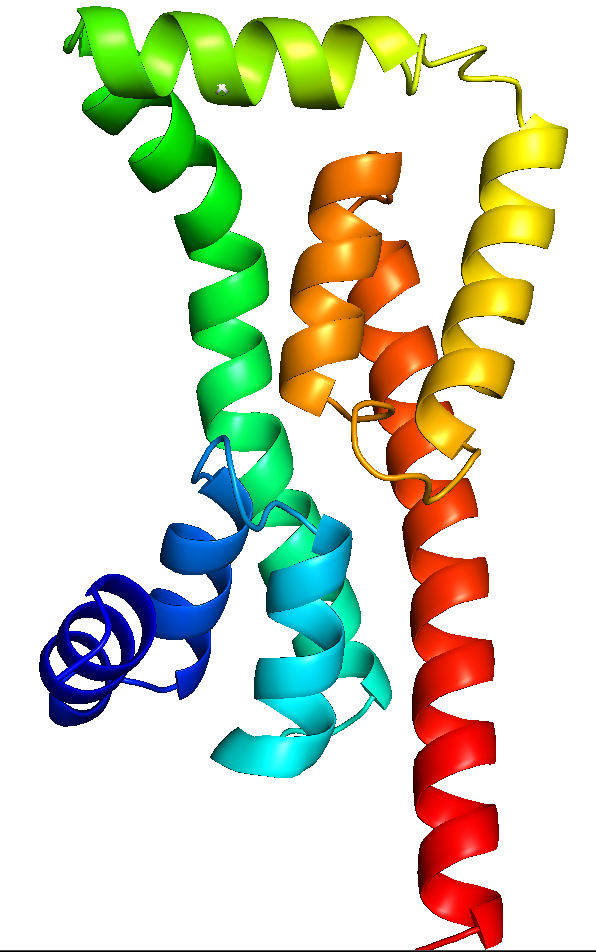
\includegraphics[width=\linewidth]{Results/w9_af.png}
  \caption{AF2 Mt2055 model}
  \label{fig:w9_af}
\end{subfigure}\hfil % <-- added
\caption{AlphaFold2 Modelling}
\small
Rainbow spectrum: N-terminal blue to C-terminal red.
\label{fig:af2_modelling}
\end{figure}


AF2 also gave rise to the opportunity to make structural predictions for another prominent member of the PF09335 family; Vmp1.  Attempts to model Vmp1 with Rosetta methods did not result in sensible models, even the DedA domain could not be modeled within the context of Vmp1.  Vmp1 is a 406 residue protein and Tmem41b forms complexes \emph{in vitro} and \emph{in vivo} with this other possible Atg protein \cite{Mizushima2011}. Molecular interaction of
Tmem41b is not detected with other Atg proteins. Tmem41b knockout cells exhibit inhibition of autophagosome formation and accumulation of lipid droplets \cite{Moretti2018} \cite{morita2018genome} Phenotypically Vmp1 knockout cells (KO) resemble Tmem41b KO cells indicating functional redundancy. Exogenous expression of the respective protein in the knockout cells restores function and the overexpression of Vmp1 in Tmem41b knockout cells restores autophagic flux with the reverse not being true \cite{Moretti2018}.

Examination of the Respre predicted contact map for Vmp1 (figure \ref{fig:vmp1}) predicts there is a bundle of three transmembrane helices on both the N-erminal and C-terminal sides of the conserved DedA structural domain.  Analysing the contact features of the DedA domain indicates an atypical pattern when comparing the equivalent region of the contact maps to other PF09335 homologues; the internal symmetry is broken. In the case of the C-terminal side of the DedA domains of Vmp1 the contact map can be interpreted in line with other PF09335 homologues displaying the common features as expected. However, the contact map features for the N-terminal symmetric half show a thirty-residue insertion between the first re-entrant loop and the proceeding transmembrane helix.  Here it can be seen that the TM helix simultaneously makes contact with the insertion and the C-terminal half of the re-entrant loop.  The insertion is highly conserved; this can be seen by the Consurf conservation mapping on the diagonal of the Vmp1 contact map.  The existence of this insertion could explain why Vmp1 is able carry out its function in the absence of Tmem41b while the reverse is not possible; the insertion may be a structurally essential feature not present in Tmem41b. The experimental evidence suggests that Vmp1 and Tmem41b oligomerise. It is possible that both homo-oligomers and hetero-oligomers form but only those where Vmp1 is present result in a functional protein.  

\begin{figure}[th!]
    \centering
    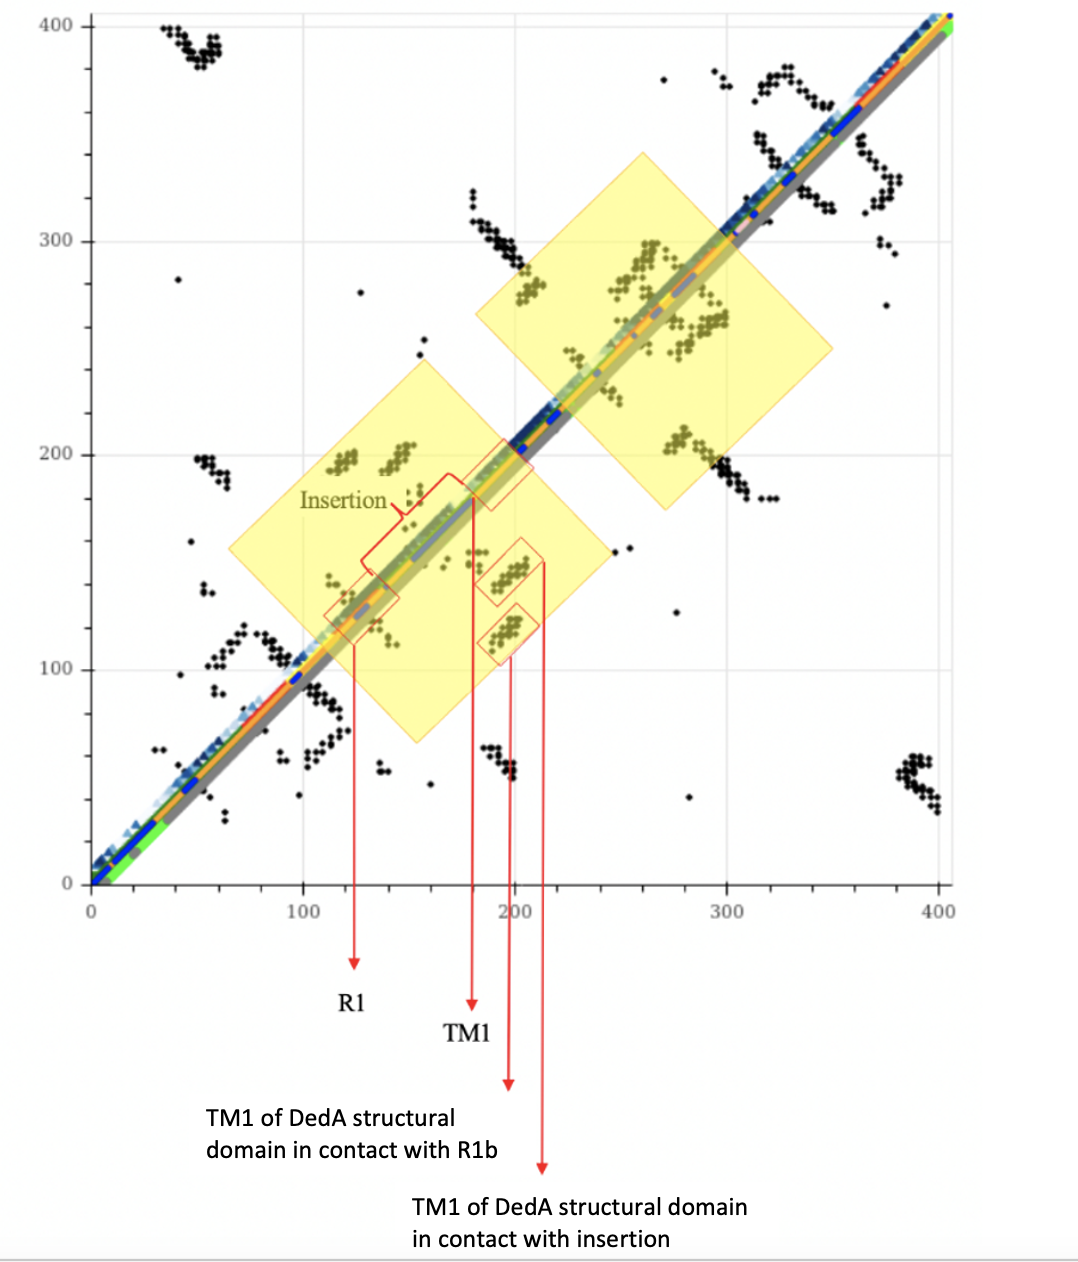
\includegraphics[width=150mm, scale =0.5]{Results/vmp1.png}
    \caption{Enhanced contact map for Vmp1}
    \label{fig:vmp1}
    \small
    Vmp-1 contact map constructed using DeepMetaPSICOV with additional information overlaid on the
diagonal. The outer diagonals show the TOPCONS membrane prediction (red regions being predicted TM helices, green; inside cell, yellow; outside). The thin central diagonal is the secondary structure prediction (orange, helix; blue, coil). Additionally, there is a blue spectrum diagonal which indicates levels of conservation from Consurf \cite{Ashkenazy2016} (the darker the blue the higher the level of conservation). Also, the grey (ordered) and lime green (disordered) diagonal utilises disorder predictions from IUPRED2a \cite{Meszaros2018}. R1 is the N-terminal re-entrant loop; R1b is the C-terminal half of the N-terminal re-entrant loop.
\end{figure}

Modelling of Vmp1 using AF2 produced a  model where most regions have a high pLDDT scores (Figure \ref{fig:vmp1_af}).  The model reveals three transmembrane helices upstream not in contact with each other and one downstream from the DedA domain.  This is in contrast to the predicted contact map where three transmembrane bundles are expected on both sides of the DedA domain. The familiar DedA domain features are clearly visible but with some differences.  Firstly, the N-terminal side amphipathic helix of the DedA domain is missing and an additional amphipathic helix is present on the C-terminal side of the DedA structural domain.  Secondly there is a loop region between the first re-entrant loop and the proceeding transmembrane helix, placing this region at the entrance of a putative channel.  The loop region corresponds to the insertion highlighted in the examination of the contact map, however, as opposed to the interpretation of the predicted contact map, in the AF2 model the loop insertion is not in contact with the proceeding transmembrane helix as the contact map suggested (Figure \ref{fig:vmp1_topt}). 


\begin{figure}[th!]
    \centering
    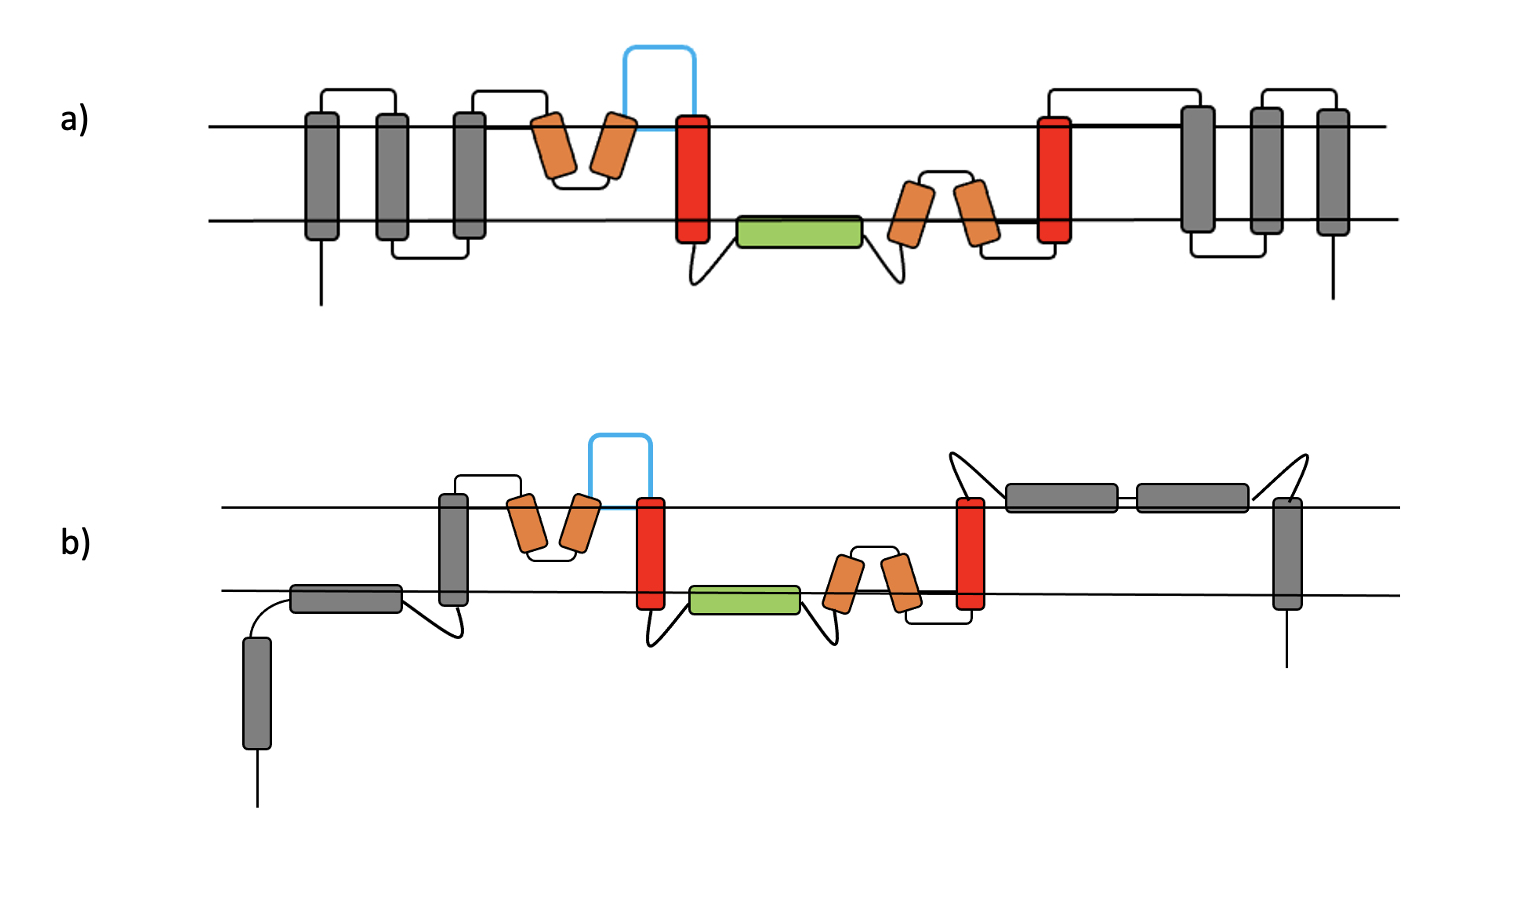
\includegraphics[width=170mm, scale =1]{Results/vmp1_topo.png}
    \caption{Topology of Vmp1 derived from the AF2 model}
    \label{fig:vmp1_topt}
    Grey: Helices that are additional to the established DedA core; red: TM helices belonging to the established DedA domain; orange; re-entrant loops belonging to the established DedA domain; green: amphipathic helices belonging to the established DedA domain; Blue: Highly conserved DedA domain loop insert.  a) Vmp predicted topology derived from predicted contact map analysis.  The presence of the amphipathic helix cannot be extrapolated from the predicted contact map, it's presence here is assumed based on helical secondary structure prediction and reference to the DedA domain topology to homologues.  The absence, compared other members of the DedA superfamily, of the N-terminal side amphipathic helix is assumed to to the lack of helix seconary structure allocation in this region.  b) Vmp predicted topology derived from predicted AF2 structure analysis.
    \small
    
\end{figure}


The discrepancy between the model and the interpretation of the ResPre predicted contact map can be explained by the fact that if the protein exists in multiple conformations, the contact map would be a superpostion of all the alternative conformations; the AF2 would be a representation of one of these conformations.  Additionally comparing predicated contact maps derived from alternative methods show that there is a lack of consistency between the various algorithms being used to generating co-variance data for Vmp1.

Further structural examination of the loop insertion modelled by AF2 was limited as unfortunately the local quality pLDDT scoring for this region is low.  ConSurf mapping of residue conservation for the insertion loop shows highly conserved regions along this structure. HHpred was used to query the PDB with the sequence making up the length of the mysterious loop, however, no hits were reported.

\begin{figure}[th!]
    \centering
    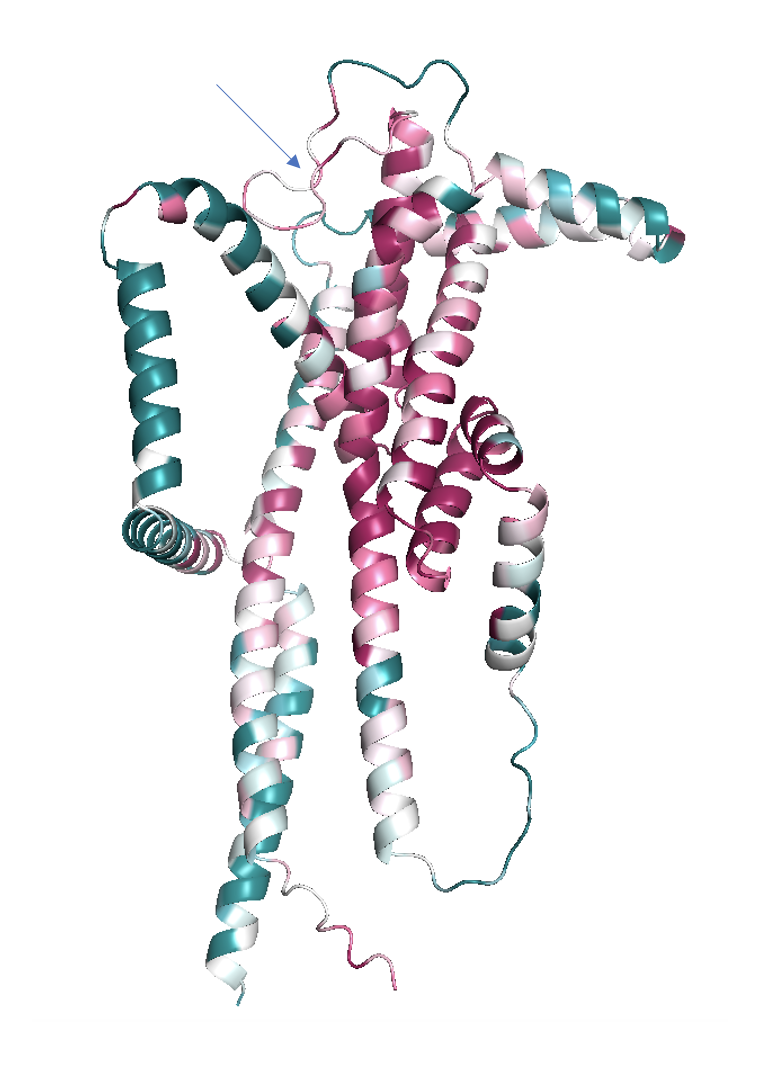
\includegraphics[width=100mm, scale =0.5]{Results/vmp1_af_consurf.png}
    \caption{Vmp1 AF2 model with ConSurf conservation mapping }
    \label{fig:vmp1_af}
    \small
    Arrow indication to conserved loop region.
\end{figure}

Examination of the N-terminal half contact map features of the AF2 Vmp1 model does show poor correlation with the predicted contact of the same region (Figure \ref{fig:vmp1_af_cmap}).  This indicates the N-terminal half may not be a valid structural prediction.  Vmp1 is part of the DedA family but with an atypical N-teminal domain.  AF2 uses the MSA to aid the modelling; any deep MSA will contain other members of the DedA family thereby maybe introducing noise into the N-terminal domain.  The introduction of this noise could impact on modelling in this region.  The introduction of noise through generation of deep MSAs built using a metagenomic database (during a separate piece of research - data not shown) has been shown result in contact signal loss and consequent decrease in model accuracy.

\begin{figure}[th!]
    \centering
    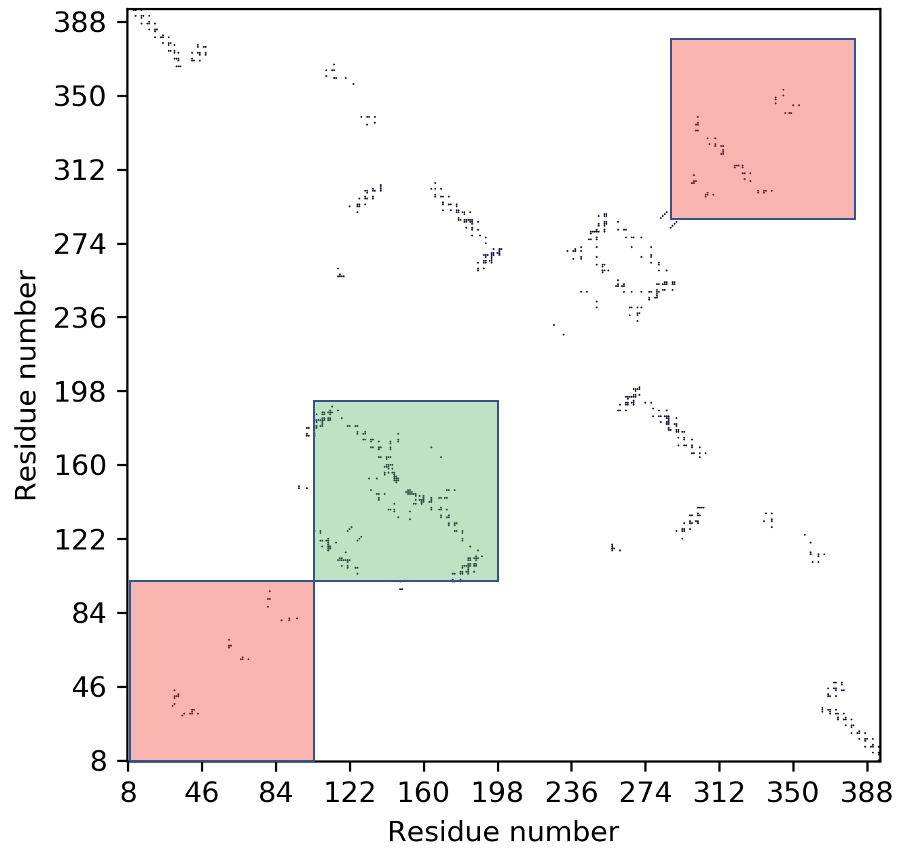
\includegraphics[width=100mm, scale =0.5]{Results/af_vmp1_cmap.png}
    \caption{Vmp1 AF2 model contact map}
    \label{fig:vmp1_af_cmap}
    \small
    Red boxes highlight missing three-helical bundles present on predicted contact map. Green box highlights N-terminal hald of DedA domain where the AF2 model contact features do not correlate with the predictions.
\end{figure}


\section{Potential homology between the DedA family and ABC transporters}
Performing a HHpred search with the Tmem41b sequence against the full PDB results in a strong hit against the Type I ABC transporter 3d31C. The hit has a 90\% probability and is across the whole length of the sequence.  This finding along with the ABC transporter structural hit with models where the re-entrant loop is forced into a transmembrane conformation points to the possibility that DedA proteins maybe related to ABC transporters.   A similar link has been suggested for the transmembrane autophagy protein Atg9 where the N- and C- terminal domains share membrane and tertiary topology (i.e. have a repeat) with sequence similarity identified locally around proline residues in the re-entrant loops and sequence similarity to N- terminal region of the transmembrane domains of T1 ABC exporters \cite{zhang2021evolution}.\\

A comparison of the proposed topology of Tmem41b with the topology of 3d31C (figure \ref{fig:abc_topology}) does indeed support an evolutionary link between the two where one side of the re-entrant loop has flipped forming a straight transmembrane helix or alternatively one half of the transmembrane helix has flipped forming a V-shaped re-entrant loop.  This 'flipping' has been shown previously in CPA/AT transporters \cite{sudha2021evolutionary}.

\begin{figure}[th!]
    \centering
    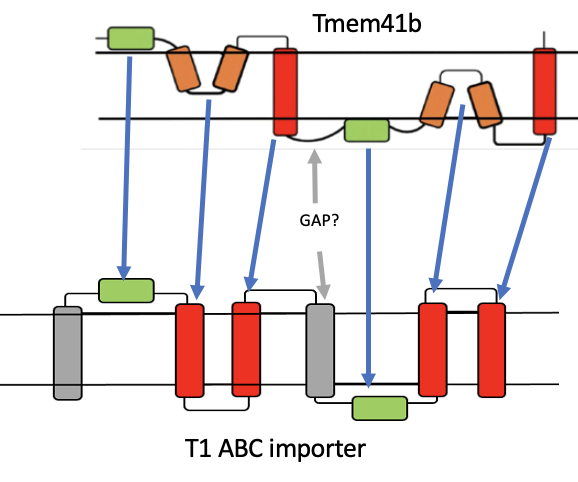
\includegraphics[width=100mm, scale =0.5]{Results/topology_comparison.png}
    \caption{Comparison of topologies of Tmem41b and 3d31C}
    \label{fig:abc_topology}
    \small
\end{figure}

However, analysis of the HHpred alignment (figure \ref{fig:abc_aln}) does reveal that the structural features do not correspond with each other in sequence indicating that the HHpred hit was a chance hit.

\begin{figure}[th!]
    \centering
    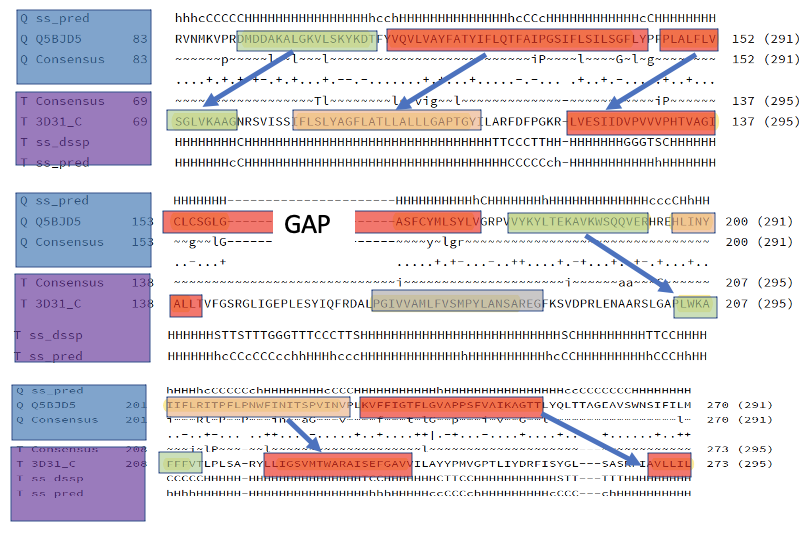
\includegraphics[width=100mm, scale =0.5]{Results/3d31c_aln.png}
    \caption{Annotated HHpred alignments of Tmem41b and 3d31C}
    \label{fig:abc_aln}
    \small
\end{figure}



\section{Conclusions}
Sequence, co-variance and ab initio modelling analyses show that the Pfam PF09335 and PF06695 domains are distantly homologous. These domains contain a structural core composed of a pseudo-inverse repeat of an amphipathic helix, a re-entrant loop and a TM helix. All PF09335 homologues contain this central core with additional TM- helices flanking either side.

Since the publication of this material \cite{mesdaghi2020silico}, the predictions made during this investigation in regard to the presence of re-entrant loops have been experimentally verified by cysteine accessibility method (SCAM) analysis for both Tmem41b \cite{okawa2021evolution} and Yqja \cite{scarsbrook2021topological}.  The presence of re-entrant loops in a transmembrane protein strongly indicates a transporter or pore functionality since this structural feature has, hitherto, only been found in proteins of this kind \cite{Yan2010} . The structural similarities between the DedA proteins and the Cl\textsuperscript{-}/H\textsuperscript{+} antiporters raise the possibility that the families studied here are, in fact, unsuspected distant homologues having several structural features in common. In that regard it is relevant to recall a hypothesis that DedA proteins are H\textsuperscript{+} antiporters as concluded from site-directed mutagenesis (SDM) experiments \cite{Kumar2014} \cite{Kumar2016}.

Querying the models against the PDB using DALI did not yield any significant hits. However, analysis of the prediction data revealed two features of DedA proteins that independently suggest that they are secondary transporters: both an inverted repeat architecture and the presence of a re-entrant loop, which are both independently and strongly associated with transporter function \cite{Duran2013} \cite{Yan2010}. Additionally, the fact that DedA proteins show structural similarities with H\textsuperscript{+} antiporters indicate that these proteins may also couple substrate transport with an opposing H\textsuperscript{+} current. Indeed, the YqjA homologue also contains strategically placed residues known to be involved in H\textsuperscript{+} antiporter activity. The ab initio models show that the essential residues come together in the region that would be buried in the membrane potentially forming a substrate chamber consistent with the transport of a specific substrate. Further research needs to be carried out to determine what this substrate is and confirm the mechanism of transport.

The investigation into Tmem41b demonstrates how covariance prediction data have multiple roles in modern structural bioinformatics: not just by acting as restraints for model making and serving for validation of the final models but by predicting domain boundaries and revealing the presence of cryptic internal repeats not evidenced by sequence analysis. Furthermore, contact map features were characterised and proven to be a re-entrant helix signal.  This ability to characterise contact map features in relation to re-entrant loops, was very exciting at the time as it gave the possibility to allow detection of this feature in other protein families by contact map analysis.  However, the acceleration in the advancement of ab initio modelling techniques such as AF2 has to some extent superseded the idea of using contact map features to predict the presence of structural features in uncharacterised proteins from contact maps; AF2 model databases can now be mined with query structures using methods like DALI, making the search for the contact map features obsolete.







\chapter{\emph{Modelling of Atg9}}
\section{Background}
The use of covariance methods to successfully predict key structural features that are possessed by the autophagy transmembrane protein Tmem41b and its DedA homologues led to the identification of another transmembrane autophagy protein to potentially structurally characterise; Atg9.  Like Tmem41b and Vmp1, Atg9 has been shown to function in the initiation stage of autophagasome formation at the endoplasmic reticulum \cite{Zhuang2017} and its structure and molecular physiological role was a mystery.

In autophagy, Atgs are proteins involved in autophagosome construction.  Atg9 is the only transmembrane Atg protein and is the first protein of the core autophagy machinery to arrive at the site of autophagosome construction.  Atg2 receives lipids from the endoplasmic reticulum (ER) and relays them to Atg9 which moves lipids between outer and inner layers of liposomes  resulting in growth of the phagophore which develops into an autophagosome \cite{sawa2020reconstitution,yamamoto2012atg9}.  Atg9 deficiency results in phenotypical features including abnormal ER expansion \cite{zhuang2017atg9}, cellular growth defects and impaired phagocytosis \cite{tung2010loss}. One copy of Atg9 is possessed by most organisms, however, there are examples of species where Atg9 has not been identified at all for example in Alveolata species \cite{aslan2017comparative,rigden2009autophagy}. There are two human Atg9 homologues; Atg9a and Atg9b.  Atg9b is restricted to fetal tissues as well as being present in placental tissues and tissues of the testes \cite{kusama2009comprehensive}. Atg9b has also be identified in certain cancer cell lines \cite{ma2017role,yun2020wnt}.  Atg9a is the predominant form and was the subject of the attempted structural characterisation described in this chapter.  Atg9 also functions as a regulator of the innate immune system where it attenuates the actions of STING thereby depressing the immune PRR/TBK1/IRF3 axis pathway \cite{imanishi2019reciprocal}.

Previous studies have shown that Atg9 is a multi-spanning transmembrane protein and have indicated that both the N- and C-termini are cytosolic with predictions that Atg9 possesses six transmembrane helices \cite{Young2006}. 


\section{Specific Methods}
\subsection{Transmembrane prediction}
TMHMM \cite{krogh2001predicting} was used to predict transmembrane helix regions of Atg9.  Although other methods such as TopCons are known to be more accurate \cite{Tsirigos2015}, TMHMM reports the probability that a region is in fact transmembrane rather than outputting a binary 'yes/no' designation.  The probability reporting feature of TMHMM was important here as there was the possibility of the presence of an unsuspected transmembrane helix within the accepted topology of Atg9. TMHMM uses algorithms for parameter estimation and transmembrane helix region prediction by utilising hidden Markov models (HMMs) describing hydrophobicity, charge bias, helix lengths, and grammatical constraints. 

\subsection{Homology modelling}
The potential homology between Atg9 and the transmembrane domain of Type I ABC transporters was used to construct homology models which provided potentially useful 3-D structures. The software Modeller \cite{eswar2006comparative} was used to predict the structure for Atg9 based on its sequence alignment with the transmembrane domain of two HHpred hits of Type I ABC transporters. Modeller used the sequence alignments as an input in addition to the atomic coordinates of the transmembrane domain of Type I ABC transporters, and a script file.  The script file loaded the 'AutoModel' class, created an 'AutoModel' object, and set the parameters to guide the model building procedure. The script also named the 'alnfile' that contained the Atg9-ABC alignment (in the PIR format) as well as defining the known ABC structure in the alignment file.  The last line of the script file called the make method and constructed the models. The output of Modeller was a calculated model containing all non-hydrogen atoms.  The validity of the models were evaluated by calculating the ResPre \cite{yang2019genetic} predicted contact satisfaction for the top L contacts. 

\subsection{Screening PDB for ABC Transporters}
A python script was written that search for and identified the key words 'ABC' or 'CASSETTE' in the title line of each of the PDB files of the PDB.  This resulted in 51 ABC structures being detected and being the approximate number of ABC transporters present in the PDB reported in the literature 
\cite{wilkens2015structure,hegedHus2021alphafold2}.

\section{Sequence Analysis}
Initial HHpred screening of the Atg9 sequence against the PDB \cite{Burley2018} using HHpred \cite{Zimmermann2018} reveals strong hits for the transmembrane domain (TMD) region with a number of several ABC transporters with the alignments covering the putative transmembrane domain of Atg9. The HHpred probabilities ranged from 50-20\%.  Additionally, all the ABC hits clustered at the top of the probability ranked results.

ABC transporters are a large superfamily \cite{rees2009abc} of integral membrane proteins that can be subdivided into a number of classes that show a high level of conservation in their nucleotide binding domains (NBDs).  The conservation of the NBD is in contrast to the transmembrane domain regions where great diversity is present in terms of both sequence and structure \cite{rees2009abc}. 

In order to assess the similarity of the transmembrane domains from the cluster of HHpred Atg9 ABC transporter hits, a Dali \cite{Holm2016} all-against-all comparison for these structures was performed.  The resulting Z-scores ranged from 19.5-31.3, showing clear structural similarity between these hits (figure \ref{fig:abc_comp}) supporting the idea that the Atg9 ABC transporter hits are probably not chance occurrences. 

%width=\textwidth
\begin{figure}[th!]
    \centering
    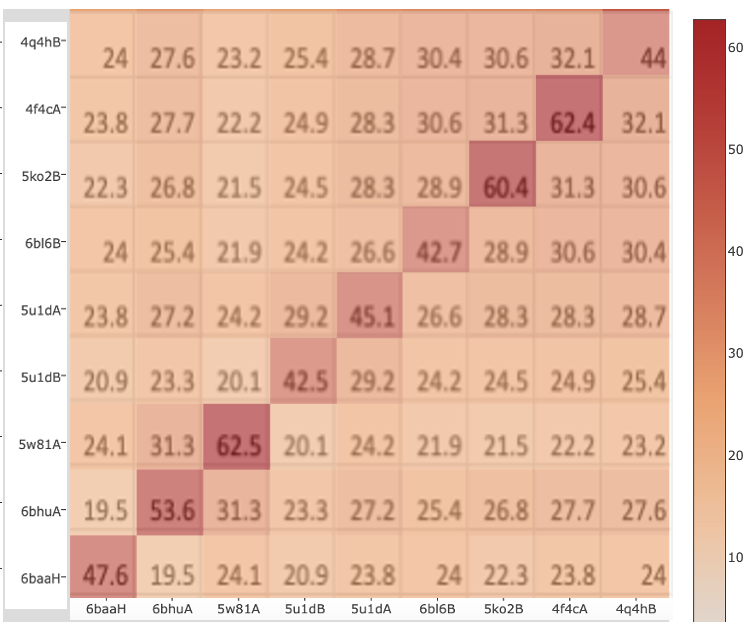
\includegraphics[width=90mm, scale=0.9]{Modelling of Atg9/abc_fold_comparison.png}
    \caption{Structural Alignments of ABC Transporter Hits}
    \label{fig:abc_comp}
    \small
    %Rosetta Ab initio Membrane model (magenta) structurally aligned with 5lilA (green).
\end{figure}


Querying the ABC transporters identified by HHpred against the Evolutionary Classification of Domain Boundaries (ECOD) database \cite{Cheng2014} indicated that all the ABC transporter hits were of Type 1 (Table \ref{ecod1}). 

\begin{table}
\caption{ECOD ABC Comparison}
\resizebox{\columnwidth}{!}{%
\centering
\arrayrulecolor{black}
\begin{tabular}{!{\color{white}\vrule}l!{\color{black}\vrule}l!{\color{black}\vrule}l!{\color{black}\vrule}l!{\color{black}\vrule}l!{\color{black}\vrule}l!{\color{black}\vrule}} 
\hline
\rowcolor[rgb]{0.267,0.447,0.769} \multicolumn{1}{!{\color{white}\vrule}c!{\color{black}\vrule}}{\textcolor{white}{\textbf{Domain ID~}}} & \multicolumn{1}{c!{\color{black}\vrule}}{\textcolor{white}{\textbf{X Group Name~}}} & \multicolumn{1}{c!{\color{black}\vrule}}{\textcolor{white}{\textbf{H Group Name~}}} & \multicolumn{1}{c!{\color{black}\vrule}}{\textcolor{white}{\textbf{T Group Name~}}} & \multicolumn{1}{c!{\color{black}\vrule}}{\textcolor{white}{\textbf{F Group Name~}}} & \multicolumn{1}{c!{\color{black}\vrule}}{\textcolor{white}{\textbf{Protein Name~}}}  \\ 
\hline
\rowcolor[rgb]{0.812,0.835,0.918} e5w81A4                                                                                                & Type II ABC exporter TMD fold                                      & Type I ABC exporter TMD fold                                       & Type I ABC exporter TMD fold                                       & ABC\_membrane                                                                       & Cystic fibrosis TM conductance regulator                                  \\ 
\hline
\rowcolor[rgb]{0.914,0.922,0.961} e4q4hA1                                                                                                & Type II ABC exporter TMD fold                                      & Type I ABC exporter TMD fold                                       & Type I ABC exporter TMD fold                                       & ABC\_membrane                                                                       & ABC transporter                                                                      \\ 
\hline
\rowcolor[rgb]{0.812,0.835,0.918} e4f4cA3                                                                                                & Type II ABC exporter TMD fold                                      & Type I ABC exporter TMD fold                                       & Type I ABC exporter TMD fold                                       & ABC\_membrane                                                                       & Multidrug Resistance Protein PGP-1                                                   \\ 
\hline
\rowcolor[rgb]{0.914,0.922,0.961} e3b5xA3                                                                                                & Type II ABC exporter TMD fold                                      & Type I ABC exporter TMD fold                                       & Type I ABC exporter TMD fold                                       & ABC\_membrane                                                                       & LIPID A Export ATP-binding/Permease Protein MSBA                                     \\ 
\hline
\rowcolor[rgb]{0.812,0.835,0.918} e5ko2A4                                                                                                & Type II ABC exporter TMD fold                                      & Type I ABC exporter TMD fold                                       & Type I ABC exporter TMD fold                                       & ABC\_membrane                                                                       & Multidrug resistance protein 1A                                                      \\ 
\hline
\rowcolor[rgb]{0.914,0.922,0.961} e5u1dA3                                                                                                & Type II ABC exporter TMD fold                                      & Type I ABC exporter TMD fold                                       & Type I ABC exporter TMD fold                                       & ABC\_membrane                                                                       & Antigen peptide transporter 1                                                        \\ 
\hline
\rowcolor[rgb]{0.812,0.835,0.918} e6bl6A2                                                                                                & Type II ABC exporter TMD fold                                      & Type I ABC exporter TMD fold                                       & Type I ABC exporter TMD fold                                       & ABC\_membrane                                                                       & Lipid A export ATP-binding/permease protein~MsbA                                     \\
\hline
\end{tabular}
}
\arrayrulecolor{black}
\label{ecod1}
\end{table}


Type 1 ABC transporters have transmembrane domains that are MetI-like.  The transmembrane domains of some of this group of ABC transporters are separate proteins \cite{kadaba2008high} from the nucleotide binding domain: this is exemplified by the methionine MetNI ABC transporter. This is in contrast to other type 1 ABC transporters such as ModBC and MalFGK where the NBD and TMD are one complete protein; these are generally larger and their subunits contain six transmemrane helices.  The homologous link between the two types of type 1 ABCs is recognised as the six helices correspond to the MetNI transporter where each MetI subunit is organised around a core of five transmembrane helices.  Utilising TMHMM, the Atg9 sequence was used to predict the number of TM helices (figure \ref{fig:atg9_tmhmm}).   TMHMM predicted six transmembrane helices, in line with type 1 ABC TMDs.  It should be noted that in addition to the strong predictions for the six TM helices, there was a low probability transmembrane prediction signal around residue 250. 

\begin{figure}[th!]
    \centering
    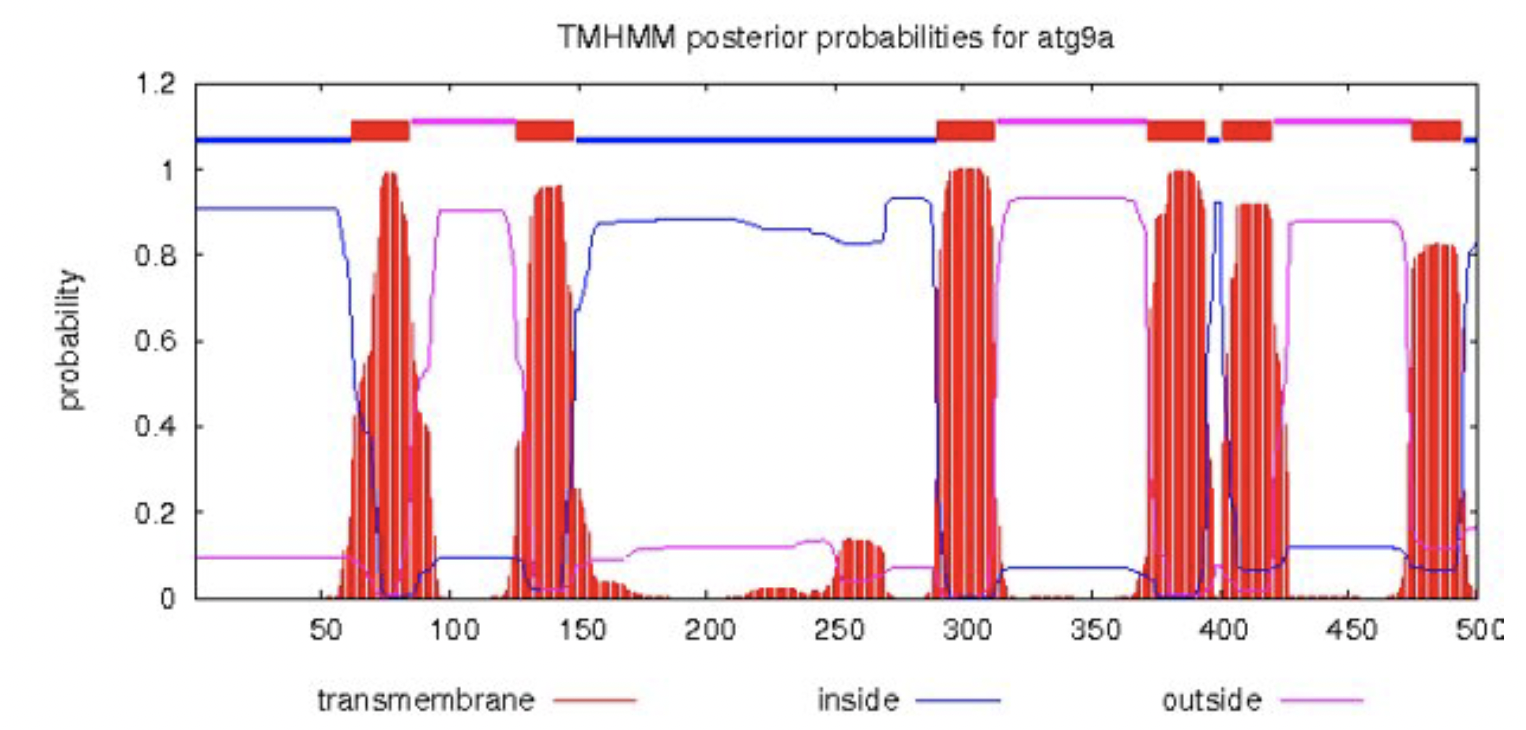
\includegraphics[width=90mm, scale=0.9]{Modelling of Atg9/atg9_tmhmm.png}
    \caption{TMHMM Prediction for TMD of Atg9}
    \label{fig:atg9_tmhmm}
    \small
    %Rosetta Ab initio Membrane model (magenta) structurally aligned with 5lilA (green).
    \label{fig:tmhmm}
\end{figure}


The combination of the HHpred probability scores and a lack of other good transmembrane protein matches in addition to the transmembrane topology prediction indicates that the Atg9 transmembrane region could very well have a Type 1 ABC transporter transmembrane domain - like fold.




To validate an ABC transporter-like fold for the putative transmembrane region of Atg9, the identification of any conserved key residues would be useful. Most ABC are transporters (importers or exporters) and all possess a nucleotide binding domain (NBD), at which hydrolysis of ATP provides the energy to drive the active transport. Atg9 does not contain the NBD sequence motifs and therefore obviously lacks NBD so unless it interacts non-covalently with an ATPase, Atg9 is not at least a conventional ABC transporter.  Conservation across the transmembrane domains of ABC transporters whose presence could be cross-referenced against Atg9 to validate the TMD ABC matches is not possible as the TMDs of the ABC superfamily are very diverse. Relating the observation of Atg9 having an ABC-like fold to its possible function is therefore not straightforward and cannot be accomplished by sequence analysis alone. Therefore, it was determined that three-dimensional modelling of Atg9 would be performed.  If modelled accurately, an ABC-like fold may be revealed, validating the ABC transporter link. 


\section{Homology Modelling}

Modeller was used to construct a homology model of the putative transmembrane domain of Atg9. The transmembrane domain of the top two HHpred hits were used as templates; 5w81 and 4q4h; with sequence similarities of 23\% and 24\% respectively. The sequence alignment was generated using ClustalW \cite{thompson2003multiple}. 

5w81 is the anion channel cystic fibrosis transmembrane conductance regulator CFTR. As with standard ABC transporters, CFTR is an active pump powered by ATP hydrolysis and possesses two transmembrane domains and two nucleotide-binding domains. CFTR is, however, atypical in that the channel gating in addition to ATP hydroysis also requires the phosphorylation of a cytosolic regulatory domain.  CFTR has two transmembrane and nucleotide-binding domains and is a single protein with each transmembrane domain containing six transmemtrane helices \cite{zhang2017conformational}. Figure \ref{fig:5w81_hmo} is the output 5w81 template homology model.


\begin{figure}[th!]
    \centering
    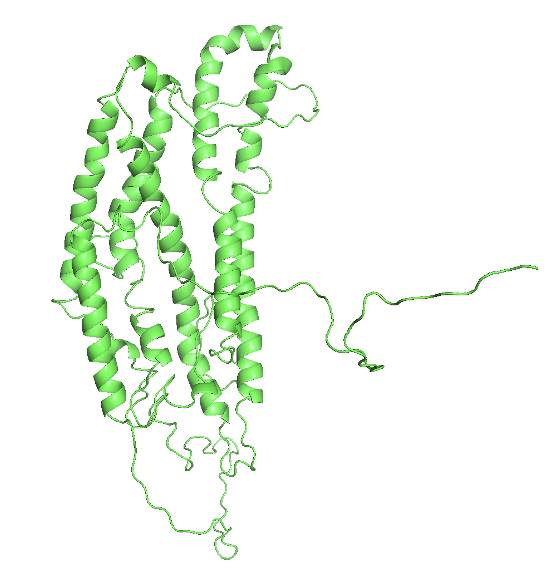
\includegraphics[width=50mm, scale=0.5]{Modelling of Atg9/atg9_hmo_5w81.png}
    \caption{Homology model for Atg9 (5w81 template)}
    \label{fig:5w81_hmo}
    \small
    %Rosetta Ab initio Membrane model (magenta) structurally aligned with 5lilA (green).
\end{figure}

\begin{figure}[htb]
    \centering % <-- added
\begin{subfigure}{0.5\textwidth}
  \includegraphics[width=\linewidth]{Modelling of Atg9/atg9_hmo_5w81_cmap.png}
  \caption{Atg9-5w81 Homology Model Contact Map}
  \label{fig:0}
  \end{subfigure}\hfil % <-- added
  \begin{subfigure}{0.45\textwidth}
  \includegraphics[width=\linewidth]{Modelling of Atg9/5w81_respre_super.png}
  \caption{Superposition of Atg9 ResPre predicted contacts with the Atg9-5w81 homology model}
  \label{fig:5w81_hom_cmap_super}
\end{subfigure}\hfil % <-- added
\begin{subfigure}{0.75\textwidth}
    \includegraphics[width=\linewidth]{Modelling of Atg9/prec_5w81_respre.png}
    \caption{Precision profile of the Atg9 5w81 homology model}
    \label{fig:prec_5w81}
\end{subfigure}\hfil % <-- added
\caption{Atg9 5w81 Homology Model Quality Determination}
\small
\label{fig:atg9_5w81_quality}
\end{figure}


\begin{figure}[th!]
    \centering
    \includegraphics[width=50mm, scale=0.5]{Modelling of Atg9/atg9_hmo_4q4h.png}
    \caption{Homology model for Atg9 (4q4h template)}
    \label{fig:4q4h_hmo}
    \small
\end{figure}

A second homology model was constructed utilising 4q4h as a template. 4q4h is the crystal structure of TM287/288 ABC exporter and, like 5w81, possesses six transmembrane helices in each TMD \cite{hohl2014structural}.  Figure \ref{fig:4q4h_hmo} shows this output homology model.

\begin{figure}[htb]
    \centering % <-- added
\begin{subfigure}{0.5\textwidth}
  \includegraphics[width=\linewidth]{Modelling of Atg9/atg9_hmo_4q4h_cmap.png}
  \caption{Atg9 4q4h Contact Map}
  \label{fig:0}
\end{subfigure}\hfil % <-- added
\begin{subfigure}{0.45\textwidth}
  \includegraphics[width=\linewidth]{Modelling of Atg9/super_atg9_hmo_4q4h.png}
  \caption{Superposition of ResPre predicted contacts with 4q4h homology model}
  \label{fig:4q4h_hom_cmap_super}
\end{subfigure}\hfil % <-- added
\begin{subfigure}{0.75\textwidth}
  \includegraphics[width=\linewidth]{Modelling of Atg9/prec_hmo_4q4h.png}
  \caption{Precision profile of the Atg9 4q4h homology model}
  \label{fig:prec_4q4h}
\end{subfigure}\hfil % <-- added
\caption{Atg9 4q4h homology model quality determination}
\small
\label{fig:atg9_4q4h_quality}
\end{figure}

Performing the predicted contact satisfaction analysis \cite{Simkovic2017} for both homology models revealed a poor contact satisfaction profile indicating that the correct fold of Atg9 was not achieved through the homology modelling exercise (figures \ref{fig:prec_5w81} and \ref{fig:prec_4q4h}).  In an effort to determine whether there were any local regions where the modelling had captured the correct fold, the contact maps derived from the ResPre \cite{yang2019genetic} predictions and the homology models were superposed (figures \ref{fig:5w81_hom_cmap_super} and \ref{fig:4q4h_hom_cmap_super}).  The superpositions did hint at common features (Figures \ref{fig:5w81_hom_cmap_super} and \ref{fig:4q4h_hom_cmap_super}).  The figures use the homology model as the reference structure; grey points are homology model contacts not present in the predicted contact map while black points are contacts present in both model and prediction; red points are contacts present in the prediction but not in the model. Analysis proved difficult; it was problematic to ascertain whether the contact map features were by virtue of alpha helical contacts and therefore not indicative of homology or whether local structural features had actually been actually correctly folded.

\section{Ab initio Modelling}
The unsuccessful Atg9 homology modelling trial led to an attempt to construct ab initio models for Atg9 in an effort to test the hypothesis that Atg9 possesses an ABC-like fold. A metagenomics-enriched database was employed to obtain as accurate as possible covariance-based contact predictions.  The use of the metagenomics database to build the MSA for Atg9 was successful in raising the Neff from 438 (using Uniprot) to 843 for the whole protein. The sequence coverage profile showed that the number of sequences in the MSA covering the C-terminal side after position remain low (Figure \ref{fig:atg9_msa}).  The boundary at position 500 represents the end of the first domain; indeed, HHpred alignments of Atg9 show the Type I ABC transporters transmembrane domains matching with this first putative domain.  Calculating the Neff values for this first domain gave values of 554 when using Uniprot and 1024 when utilising the metagenomics database. JackHMMER \cite{Johnson2010} was then used to generate the MSAs and ResPre \cite{Li} to make the contact predictions based on the metagenomics enhanced MSAs for the putative transmembrane domain of Atg9.  The predicted contact information was then used as restraints to construct models using both Rosetta ab initio and RosettaMembrane protocols.  TopCons transmembrane predictions were also used as restraints for RosettaMembrane model building.  One thousand models of each were constructed and each of the thousand were clustered using Spicker; the centroid of the largest cluster was selected as the top model.  RosettaMembrane models contained a number of larger clusters with the maximum cluster size being 200 and the smallest cluster being 68.  This is in contrast to the clustering of the Rosetta ab initio models where cluster sizes were much smaller with the maximum cluster size being five and the smallest clusters being only two, indicating that the output models did not converge on a consensus energetic minimum.  

\begin{figure}[htb]
\begin{subfigure}{0.5\textwidth}
  \includegraphics[width=\linewidth]{introduction/atg9_mas_uni.png}
  \caption{Atg9 Uniprot MSA coverage}
  \label{fig:0}
\end{subfigure}\hfil % <-- added
\begin{subfigure}{0.5\textwidth}
  \includegraphics[width=\linewidth]{introduction/atg9_msa_meta.png}
  \caption{Atg9 metagenomic MSA coverage}
  \label{fig:1}
\end{subfigure}\hfil % <-- added
\caption{Atg9 MSA Sequence coverage profiles}
\small
\label{fig:atg9_msa}
\end{figure}

The output models from the RosettaMembrane flavour appeared more plausible compared to the outputs from Rosetta ab initio;  these models possessed helices packed together in such a way that they could conceivably sit in a membrane bi-layer.  Indeed running the top model against the PDB using DALI did result in three ABC transporter hits albeit of the Type II class; 6quz-D (z=3.9), 2lw1-A (z=5.4),  and 4MRN-B (z=6).  Despite the fact that the resultant RosettaMembrane models appeared visually promising and good PDB structural hits with ABC transporters, quantitative analysis of both the Rosetta ab initio and the RosettaMembrane  structural predictions resulted in poor precision scores (Figure \ref{fig:atg9_ab_models}) indicating that the correct fold had not been predicted \cite{DeOliveira2016}.

\begin{figure}[htb]
    \centering % <-- added
\begin{subfigure}{0.25\textwidth}
  \includegraphics[width=\linewidth]{Modelling of Atg9/atg_ros_ab.png}
  \caption{Rosetta Ab initio model of Atg9 TMD}
  \label{fig:0}
\end{subfigure}\hfil % <-- added
\begin{subfigure}{0.25\textwidth}
  \includegraphics[width=\linewidth]{Modelling of Atg9/prec_ros.png}
  \caption{Precision profile of Rosetta Ab initio model of Atg9 TMD}
  \label{fig:0}
\end{subfigure}\hfil % <-- added
\begin{subfigure}{0.25\textwidth}
  \includegraphics[width=\linewidth]{Modelling of Atg9/atg_ros_mem.png}
  \caption{RosettaMembrane model of Atg9 TMD}
  \label{fig:1}
\end{subfigure}\hfil % <-- added
\begin{subfigure}{0.25\textwidth}
  \includegraphics[width=\linewidth]{Modelling of Atg9/prec_rosmem.png}
  \caption{Precision profile of Rosetta Ab initio model of Atg9 TMD}
  \label{fig:0}
\end{subfigure}\hfil % <-- added
\caption{Ab initio modelling of Atg9}
\small
Precision score evaluation of the Rosetta ab initio and RosettaMembrane model in relation to the predicted contacts at various contact cutoff values are shown where L = sequence length (rounded down to the nearest whole number of contacts). The 50\% precision cut off is shown (blue line) as a visual marker. A minimum of 70\% contact satisfaction for the top L contacts would be suggestive of good quality models \cite{DeOliveira2016}.
\label{fig:atg9_ab_models}
\end{figure}

\section{Contact Map Analysis}
Efforts to obtain evidence of Atg9 and Type I ABC tranporter transmembrane domain homology independent of the HHpred results using homology and ab initio modelling did not yield convincing data.  In the case of ab initio modeling this was to be expected as trying to make accurate structural prediction for a 500 residue protein was, at the time, uncommon as large complex proteins present a convergence challenge for ab initio structure prediction (Figure \ref{fig:croem_vs_5w81}). The idea of successful ab initio modelling was relying heavily on the contact predictions acting as restraints.  Knowing that the contact predictions are very reliable an alternative tool was identified that could screen the PDBTM utilising the contact information by passing the need to structurally predict the structure of Atg9; MapAlign \cite{Ovchinnikov2017}. 

MapAlign was developed in 2017 by the Baker group as a tool to refine the structures of ab initio models.  MapAlign was used to identify contact map feature matches to known structures and aid the modelling of large and complex proteins that otherwise would be a challenge for ab initio structure prediction. MapAlign exploits the fact that structural matches can be detected by covariance analysis in the absence of detectable sequence similarity since structural similarity is retained over larger evolutionary distances.  MapAlign was used to screen predicted contacts against of the PDB; performing contact-based structure matching by comparing contact maps of the query and target and attempting to align predicted contacts with the contact patterns of experimental structures then highlighting any structural matches. In its original implementation, the matches were then used to refine the ab initio models.  MapAlign compares two contact maps and returns an alignment that attempts to maximize the number of overlapping contacts at the same time as attempting to minimise the number of gaps.

MapAlign was employed to screen the predicted contacts of the putative transmembrane domain of Atg9 against a library of non-redundant PDBTM structures. The input contact predictions for Atg9 were filtered to leave only the medium (above six residues apart) and long range (above twelve residues apart) contacts; this step was taken as the successful usage of MapAlign by the GREMLIN group only utilised these sets of predicted contacts when employing this contact map alignment tool \cite{Ovchinnikov2017} and therefore may have been optimised for these contact categories. 

MapAlign provided a list of the 25 top hits ranked by the MapAlign score (a combination of contact satisfaction and gap penalties).  The top 25 results listed PDBTM hits that seemed not to be related in any way and there was no clustering of related proteins at the top of the list.  Within the top 25 hits there were, however, six ABC transporter hits (Figure  \ref{table:map_align_eco}) that, according to the Evolutionary Classification of Protein Domains (ECOD), were all of the Type II class.

\begin{table}
\caption{ECOD classification comparison of the ABC transporter MapAlign hits}
\resizebox{\columnwidth}{!}{%
\centering
\arrayrulecolor{black}
\begin{tabular}{!{\color{white}\vrule}l!{\color{black}\vrule}l!{\color{white}\vrule}l!{\color{white}\vrule}l!{\color{white}\vrule}l!{\color{white}\vrule}l!{\color{white}\vrule}} 
\hline
\rowcolor[rgb]{0.267,0.447,0.769} \multicolumn{1}{!{\color{white}\vrule}c!{\color{black}\vrule}}{Domain ID~} & \multicolumn{1}{c!{\color{white}\vrule}}{X Group Name~} & \multicolumn{1}{c!{\color{white}\vrule}}{H Group Name~} & \multicolumn{1}{c!{\color{white}\vrule}}{T Group Name~} & \multicolumn{1}{c!{\color{white}\vrule}}{F Group Name~} & \multicolumn{1}{c!{\color{white}\vrule}}{Protein Name~}                \\ 
\hline
\rowcolor[rgb]{0.812,0.835,0.918} e5l22A2                                                                    & Type II ABC exporter TMD fold          & Type I ABC exporter TMD fold           & Type I ABC exporter TMD fold           & ABC\_membrane                                           & ABC transporter (HlyB subfamily)                                       \\ 
\hline
\rowcolor[rgb]{0.914,0.922,0.961} e5mkkA2                                                                    & Type II ABC exporter TMD fold          & Type I ABC exporter TMD fold           & Type I ABC exporter TMD fold           & ABC\_membrane                                           & Multidrug resistance ABC transporter ATP-binding and permease protein  \\ 
\hline
\rowcolor[rgb]{0.812,0.835,0.918} e5eg1A2                                                                    & Type II ABC exporter TMD fold          & Type I ABC exporter TMD fold           & Type I ABC exporter TMD fold           & ABC\_membrane                                           & Microcin-J25 export ATP-binding/permease protein McjD                  \\ 
\hline
\rowcolor[rgb]{0.914,0.922,0.961} e4aywA2                                                                    & Type II ABC exporter TMD fold          & Type I ABC exporter TMD fold           & Type I ABC exporter TMD fold           & ABC\_membrane                                           & ATP-BINDING CASSETTE SUB-FAMILY B MEMBER 10                            \\ 
\hline
\rowcolor[rgb]{0.812,0.835,0.918} e4mrnA1                                                                    & Type II ABC exporter TMD fold          & Type I ABC exporter TMD fold           & Type I ABC exporter TMD fold           & ABC\_membrane                                           & ABC TRANSPORTER RELATED PROTEIN                                        \\ 
\hline
\rowcolor[rgb]{0.914,0.922,0.961} e3wmfA2                                                                    & Type II ABC exporter TMD fold          & Type I ABC exporter TMD fold           & Type I ABC exporter TMD fold           & ABC\_membrane                                           & ATP-binding cassette, sub-family B, member 1                           \\ 
\hline
\rowcolor[rgb]{0.812,0.835,0.918} e4ry2A3                                                                    & Type II ABC exporter TMD fold          & Type I ABC exporter TMD fold           & Type I ABC exporter TMD fold           & ABC\_membrane                                           & ABC-type bacteriocin transporter                                       \\
\hline
\end{tabular}
}
\label{table:map_align_eco}
\arrayrulecolor{black}
\end{table}

The use of the contact map alignment method MapAlign again did not provide definitive hits that would indicate a common co-evolutionary profile between Atg9 and Type I ABC transporter transmembrane domains. 

A major issue with both the ab initio modelling and attempted contact map alignment methods is that even with good co-variance information the biologically
important contacts it reveals will be a superposition of contacts from different conformational states and if it is an oligomer, intra- and inter-molecular contacts would also be present; if Atg9 is indeed an oligomeric transporter then both of these would result in noise when attempting to model or align contact maps.


\section{Analysis: Low Resolution CryoEM Model}

During the investigation into Atg9 a low resolution (7.8Å) CryoEM structure of Arabidopsis Atg9 was published \cite{Lai2020}.  The group combined contact prediction using co-evolutionary data to construct a model and claim insight into the Atg9 architecture.  The group concludes that Atg9 has six transmembrane $\alpha$-helices and forms a homotrimer where at the center, the protomers interact via their membrane-embedded and C-terminal cytoplasmic regions. 

The published material gave another possible avenue to determine the molecular function of Atg9 and whether it is related to Type I ABC transporters.  The conclusion that Atg9 forms a homo-trimer is in conflict with the possibility of the ABC transporter link as there are no ABC transporters that function by forming a trimer; although this could still be possible if Atg9 is only distantly related to ABCs and not explicitly a member of the ABC transporter super family. Careful examination of the data presented in the paper indicate that the authors' conclusions are speculative as the experimental interpretation is dependent on the bioinformatics at this resolution.  The team utilised RaptorX \cite{Ma2015} to generate the covariance-derived contact predictions, again, the paper does not show the predicted contact map to demonstrate the strength of the inter-helical predictions that are the key information that allowed them to tentatively trace the transmembrane helices. Analysing the data further presented in the paper the authors state that "the final model places C$\alpha$ of the pairwise residues are within 15 Å of each other in 43 out of the top 46 identified pairs, with an average distance of 10.2 Å. The 7\% violated C$\alpha$- C$\alpha$ distance constraints is in agreement with the observed false-positive rate in previous structure prediction studies of known protein structures using evolutionary covariance."; 15Å was a very generous threshold as contact prediction methods are usually bench-marked with C$\beta$ (not C$\alpha$) within 8Å.  This analysis leads to the possibility that the resolution of the EM-map coupled with information gained from the model of Atg9 was insufficient to dock predicted model in the map as they based their speculation from only small amounts of data. For example, in the section titled the cytoplasmic region:

'Consequently, we ascribe the remaining density in our reconstruction to largely represent the structured domains of the C-terminal regions. The estimated volume of this region is 20\% of the density of the entire protomer, which approximately corresponds to the size of a 20 kDa polypeptide and is consistent with the calculated mass of the structured domain (16 kDa). The C-terminal region forms three distinct petal-shaped features around the three-fold axis where the middle loop is tucked behind.'

The structure and the proceeding docking should have been verified; this could have been achieved by using domain (N- or C- terminal) specific antibodies to label these regions in the single particle reconstruction or alternatively use the tagging before going onto structure prediction and docking; this may have improved the particle alignments and resolution. Consequently the experimental data does not offer much constrain to the structure prediction and docking therefore it is only as good as the bioinformatic predictions that were applied.

\begin{figure}[th!]
    \centering
    \includegraphics[width=\textwidth]{Modelling of Atg9/respred_cmap_anal.png}
    \caption{Atg9 ResPre TMD Contact map analysis}
    \label{fig:respr_anal}
    \small
    The Purple box groups predicted transmembrane helical contacts that are accounted for in the Lai et al (2020) paper.  Outside of the purple box are predicted transmembrane contacts that the Lai et al (2020) model does not account for. The coloured outlines of the boxes correspond to the positions of the contacts as annotated in the contact map.
\end{figure}
In order to evaluate the bioinformatic predictions provided in the paper a metagenomic enhanced ResPre contact map with the visualisation of embedded prediction data was constructed and used to compare with the helical contacts described in the Lai et al (2020) paper \ref{fig:respr_anal}.  The authors interpretation of their low-resolution map use predicted contacts between transmembrane 1 and 2, 4 and 5 , 3 and 6, and 1 and 4, all antiparallel. However, interpretation of the enhanced ResPre contact map strongly supports an orientation between TM1 and 4 as parallel. Also, the ResPre contact data shows a parallel signal between transmembrane 2 and 3. Both the parallel assignments 2-3 and 1-4 are inconsistent with the straightforward topology presented in the paper and suggests that the C- and N- termini are on opposing sides of the membrane rather than the same side (Figure \ref{fig:respre_anal2}).  This finding prompted a further investigation into the experimental origins of the accepted topology of Atg9 \cite{Young2006}. During the research by Young (2006) they obtained experimental data for the topology of the N- and C-terminal domains using in vitro translocation into microsomes, followed by protease protection. This was possible because they had specific antibodies to the N- and C-terminus. The experimental data supported a model of 6 transmembrane helices, with both termini in the cytosol.  However, the paper does highlight some property of the putative transmembrane between TM2 and 3 which was determined not to be a transmembrane:  Lai et al (2020) also highlight this in their paper from the homology of the plant protein with myosin proteins (Figure S6). This region is also of interest as it contains a large number of conserved residues. Additionally, the data in Young (2006) is more equivocal regarding the orientation of the C-terminus and not as robust as for the N-terminus. This all gives a basis for a possible alternative topology for Atg9.

\begin{figure}[th!]
    \centering
    \includegraphics[width=\textwidth]{Modelling of Atg9/cmap_comparison_w_lai_etal.png}
    \caption{Comparison of Lai et al. low resolution interpretation with our contact data. }
    \label{fig:respre_anal2}
    \small
    a) Comparison of helical contacts with ResPre predicted helical contact features; blue boxes are helical contacts that are consistent with the proposed CryoEM model and green boxes are helical contacts that are inconsistent with the CryoEM model.  The coloured outlines of the boxes correspond to the positions of the contacts as annotated in \ref{fig:respr_anal} contact map. 'A' - parallel, 'AP' -  Anti-parallel.
    b) Established Atg9 topology.
\end{figure}

\newpage



\section{ABC Transporter Survey}
The strong co-variance data supports an alternative to the accepted topology for Atg9. The possible existence of an additional transmembrane helix between TM 2 and transmembrane 3 would satisfy the predicted contact map features. Submitting the putative transmembrane domain sequence of Atg9 to the transmembrane helix prediction tool TMHMM, does indeed show a weak signal for a predicted helix between transmembrane 2 and transmembrane 3 (Figure \ref{fig:atg9_tmhmm}). The presence of the weak TMHMM signal between predicted helices transmembrane 2 and 3 prompted an investigation into the possible
structural features that are responsible for these ‘blips’. As HHpred predicted a evolutionary link between Atg9 and ABC transporters, the sequences for experimentally solved ABC transporter structures were screened for the presence of these weak signals using TMHMM. The transmembrane domains of ABC transporters show low sequence conservation and are structurally divergent, with this diversity being related to their distinct functions. Screening the PDB (see specific methods) for ABC transporters resulted in 51 entries which can be classified into eight ABC transmembrane domain folds; Pgp, ABCG2, MalFG, BtuC, EcfT, LptFG, MacB, and MlaE \cite{srikant2020evolutionary}.  The sequences for each of the 51 entries were submitted to a local installation of TMHMM.  The TMHMM output results for each sequence were visually inspected. The screening identified ten ABC transporters with at least one weak transmembrane prediction TMHMM signal; 2ONK-C, 3WME-A, 4MRN-B, 4RYZ-A, 4TQV-A, 4TMS-C, 5DO7-A, 5MKK-B, 5NIK-J and 6AN7-D.  For each of these the TMHMM profile, predicted contact map and the crystal structure were visually cross referenced in order to identify any structural features that were the origin of the 'blip' being reported by TMHMM (Figure \ref{fig:3wme_tmhmm} shows one example - 3wme).  At the same time, contact features for the transmembrane domain of the predicted contact map were annotated to identify their representation on the actual crystal structure with the aim of cross referencing these with any common contact map features present in the Atg9 predicted contact map. 

\begin{figure}[htb]
\begin{subfigure}{0.3\textwidth}
  \includegraphics[width=\linewidth]{introduction/3wme.png}
  \caption{3wme Experimental Structure.  Colour spectrum, blue is N-terminal to red C-terminal.  Q-loop highlighted which corresponds to the position of TMHMM 'blip'.}
  \label{fig:0}
\end{subfigure}\hfil % <-- added
\begin{subfigure}{0.5\textwidth}
  \includegraphics[width=\linewidth]{introduction/3wme_tmhmm.png}
  \caption{3wme TMHMM profile}
  \label{fig:atg9_tmhmm}
\end{subfigure}\hfil % <-- added
\caption{Analysis of 3wme TMHMM profile.  Red box highlighting 'blip'. }
\small
\label{fig:3wme_tmhmm}
\end{figure}

\begin{figure}[th!]
    \centering
    \includegraphics[width=100mm, scale=1]{introduction/3wme_cmap.png}
    \caption{3wme Predicted contact map analysis.    }
    \label{fig:3wme Contact map analysis}
    \small
    Transmembrane contact map features highlighted with red boxes.  Red font indicates contacts that are not present in the contact map of the experimental structure; black font indicates that features are shared by the contact map of the experimental structure. P-parallel, AP-antiparallel, I-inside, O-outside, M-membrane. 
\end{figure}

 The ABC transporter screen identified three features in ABC transporters that are responsible for a weak TMHMM transmembrane prediction signals; the nucleotide domain binding Q-loop, the extra-cellular domain and certain periplasmic helices (Figure \ref{fig:abc_tmhmm}); none of these structural features would be expected to be present in Atg9 due to the absence of the nucleotide binding domain. Also, such as in 4tqu (Figure \ref{fig:4tqu}),  a weak TMHMM was produced for a helix that has no specific function stated in the paper \cite{maruyama2015structure}. Additionally, there are cases such as in 4yms (Figure \ref{fig:4yms}) where the TMHMM prediction does not match the actual topology; five transmembrane helices are present in the crystal structure but only three were predicted.
 
 Analysing the predicted contact map features of the transmembrane domain of the ABC transporters in order to predict the structural feature representing the TMHMM 'blip' for Atg9 revealed that most of these features can be satisfied by the interhelical interfaces in the three dimensional structure when comparing to the contact map of the crystal.  There are examples, however, where the features are not satisfied by the structure; contacts responsible for dimer formation being present as well as  small contact features that cannot be satisfied by looking at the crystal structure and are possibly as a result of an alternative conformation (Figure \ref{fig:3wme Contact map analysis}).  In conclusion, the ABC transporter survey did not provide a firm indication as to what structural feature Atg9 possesses that would produce the TMHMM 'blip'.
 
 
\begin{figure}[htb]
\begin{subfigure}{0.25\textwidth}
  \includegraphics[width=\linewidth]{introduction/4yms.png}
  \caption{4yms}
  \label{fig:4yms}
\end{subfigure}\hfil % <-- added
\begin{subfigure}{0.25\textwidth}
  \includegraphics[width=\linewidth]{introduction/4tqu.png}
  \caption{4tqu}
  \label{fig:4tqu}
\end{subfigure}\hfil % <-- added
\begin{subfigure}{0.25\textwidth}
  \includegraphics[width=\linewidth]{introduction/5do7.png}
  \caption{5do7}
  \label{fig:5do7}
\end{subfigure}\hfil % <-- added
\begin{subfigure}{0.25\textwidth}
  \includegraphics[width=\linewidth]{introduction/6an7.png}
  \caption{6an7}
  \label{fig:6an7}
\end{subfigure}\hfil % <-- added
\caption{Analysis of ABC TMHMM profiles by cross-referencing with experimental structures.}
\small
\label{fig:abc_tmhmm}
\end{figure}


\section{Analysis: High Resolution CryoEM Model}
\begin{figure}[th!]
    \centering
\includegraphics[width=\linewidth]{Modelling of Atg9/6wqz.png}
    \caption{Atg9 High resolution CryoEM model}
    \label{fig:6wqz}
    \small
    Atg9 monomer topology adapted from \cite{guardia2020structure}. Spectrum: Blue-N-terminal to red C-terminal.
\end{figure}

A second CryEM model of Atg9 was published (Figure \ref{fig:6wqz}) \cite{guardia2020structure} and in contrast to the previous published CryEM model it was high resolution at 2.9 Å.  The model revealed that Atg9 has a novel fold and is a domain-swapped homotrimer with the N- and C-terminal halves of the transmembrane domain being pseudo repeats;  consisting of two transmembrane helices and one re-entrant loop with sequence similarity identified locally around proline residues in the re-entrant loops.  The domain swapping involves  a domain of one of the subunits that extends into another subunit and interacts with the main domain of this subunit with this interaction being synonymic to that of the same domain in the monomer. In Atg9 two transmembrane helices from one monomer cross over and stack in parallel with two transmembrane helices from the neighboring monomer. The model also reveals an intricate system of cavities that are consistent with its putative role lipid in lipid transport.  Also molecular dynamics simulations predict that Atg9 has membrane-bending properties.

Comparing this high resolution accurate model to the bioinformatic work conducted for Atg9, the model did not support a six transmembrane helix topology for the transmembrane domain of Atg9.  The CryoEM model shows four transmembrane helices and two re-entrant loops. Transmembrane 1, 2, 4 and 5 (helices 2, 6, 14 and 15) were predicted correctly and transmembrane 3 and 6 (helices 11 and 19) were mis-classified and were actually revealed to be re-entrant loops.  The re-entrant loops present are atypical with the cytosolic N-terminal side extending out of the membrane by approximately 6 helical turns and a proline present at the membrane interface causing the helix to turn and run parallel before forming a loop and leaving the membrane on the same cytosolic side (Figure \ref{fig:atg9_pro}). 

\begin{figure}[th!]
    \centering
\includegraphics[width=\linewidth]{Modelling of Atg9/h_res_cro_anal2.png}
    \caption{Atg9 CryoEM Analysis}
    \label{fig:atg9_pro}
    \small
    Left: Atg9 monomer topology adapted from \cite{guardia2020structure}. Red helices are from and adjacent Atg9 forming the interface. Right: Atg9 trimer (blue are cytosolic regions, yellow are membrane embedded regions, pink are luminal regions and green are interfacial helical regions (boundaries for colouring and membrane planes obtained from the PDBTM \cite{Kozma2012}).
\end{figure}

In an effort to identify the mysterious 'blip' on the TMHMM prediction and the contact map features making contact with the 'blip', the relevant regions of the model were examined. The  TMHMM 'blip' was triggered by a short alpha helix (helix 9) on the cytosolic side of the membrane between transmembrane helix 1 and the first re-entrant loop.  The helix in question makes contact with the alpha helix that extends out of the membrane from the first N-terminal side of the first re-entrant loop (Figure \ref{fig:croem_anal1}).  Cross referencing transmembrane helical contacts in the cryoEM structure with the predicted contact map features of the transmembrane domain confirms that they are in agreement.

\begin{figure}[th!]
    \centering
    \includegraphics[width=\linewidth]{Modelling of Atg9/h_res_cro_anal1.png}
    \caption{Atg9 CryoEM Analysis}
    \label{fig:croem_anal1}
    \small
    Left: Atg9 monomer topology adapted from \cite{guardia2020structure}. Right: Respre predicted contact map for Atg9. Red boxes are regions of predicted transmembrane helices; green box is the region that contained the TMHMM 'blip'; blue boxes are regions of high sequence conservation.
    
\end{figure}

The successful CryoEM structure determination of Atg9 resulted in two models in alternate conformations.  An attempt to utilise contact predictions to indicate the plausibility of a third conformational state was carried out. The two contact maps from the alternate PDB conformation structures were compared to the predicted contact map in an effort to identify features that are present in the predicted map but not in the PDB files.  The presence of additional features might indicate that there is another conformational state as the predicted contact map will show superimposed contacts that are important from all conformational states. By subtracting away contacts explained by the known structures and getting any leftover plausible, consistent sets of strongly-predicted contacts would indicate further a biologically important conformation or, of course, contacts relating to oligomeric interfaces. Utilising ConKit the structural contacts sets of the two experimentally determined PDB structures were combined and mapped against the Atg9  predicted contact two-dimensional coordinates (Figure \ref{fig:atg9_conformation}). The Figure \ref{fig:4.16a} contact map on the left shows grey points representing the predicted contacts for Atg9, black points are the predicted contacts satisfied by structural contacts and red points are contacts present in the structure but not present in the predictions.  Three predicted contact features (pink, yellow and blue boxes) in the same area of the contact map (green) not present in the structures were identified. The corresponding regions were mapped on to Atg9 (right).  In the monomer these contacts could not be explained. Figure \ref{fig:4.16b} shows unsatisfied contacting regions from the predicted contacts mapped on to the trimer; the trimeric state accounts for the three sets of contacts not satisfied by the monomer.

\begin{figure}[htb]
    \centering % <-- added
\begin{subfigure}{0.75\textwidth}
  \includegraphics[width=95mm, scale=0.9]{introduction/cryo_cmap_anal.png}
  \caption{Superposition of CryoEM contacts for both conformations with predicted contact maps comparison.  Green shaded area indicates transmembrane region where unaccounted contacts are present. Corresponding colours of boxes on the contact map (left) are mapped on to the Atg9 monomer (right) (these shaded regions mirrored across the diagonal).  In the monomer these contacts cannot be explained.}
  \label{fig:4.16a}
\end{subfigure}\hfil % <-- added
\begin{subfigure}{0.75\textwidth}
  \includegraphics[width=85mm, scale=0.9]{introduction/cryo_cmap_anal2.png}
  \caption{Inter-chain contacts. Corresponding colours of boxes on contact map (left Figure \ref{fig:4.16a}) are mapped on to the Atg9 trimer.The trimeric state accounts for the three sets of contacts not satisfied by the monomer}
  \label{fig:4.16b}
  \small
  
\end{subfigure}\hfil % <-- added
\caption{Atg9 CryoEM Contact Analysis}
\small

\label{fig:atg9_conformation}
\end{figure}

Unfortunately, the evolutionary co-variance data did not provide any evidence for a third conformation. The predicted contact map of Atg9 is a superposition of inter- and intra-chain contacts. The PDB files contain the actual inter and intra chain contacts. The contact predictions for Atg9 were all satisfied by the actual contacts from the two Atg9 CryEM structures. Therefore, based on co-variance analysis there were no additional contacts that would be required to suggest an additional conformation.  However, examining the contact prediction map it can be seen that there are very few contact predictions for the residues after position 600. Visualising the actual contacts for 6wr4 it is true that there are few contacts for residues 600 onward, however, for the 6wqz conformation there are obviously contacts present that were never predicted.  Indeed examining the sequence coverage for both the Uniprot and metagenomic MSAs used for the co-variance analysis to construct the contact predictions for Atg9, figure \ref{fig:atg9_msa} reveals that after residue 600 there is poor sequence coverage.  The poor sequence coverage for residues after 600 indicates that there is not enough data to perform co-variance analysis here and to make contact predictions for the C-terminal end of Atg9. Therefore, the limitations in data quality mean that a third conformation cannot be ruled out.

In terms of a predicted function or a predicted characterisation of a substrate for this putative transporter further analysis was unable to determine any plausible possibilities. Conservation was mapped on to the PDB structures and regions of high conservation were visualised. The region between helix 7 and 9 along with helix 13 and 12 is highly conserved and therefore critical to structure or function (Figure \ref{fig:croem_anal1}). 

\section{Potential homology between the Atg9 and ABC transporters}

 The availability of a high resolution model gave rise to the opportunity to further examine the possibility of obtaining structural evidence to support the HHpred determined sequence similarity to Type I ABC transporters.  An attempted DALI pairwise structural alignment could not align the top HHpred PDB hit Type I ABC transporter 5w81 with Atg9.  Subsequently both structures were visualised in PyMol and the regions corresponding to HHpred alignment on both structures were highlighted (Figure \ref{fig:croem_vs_5w81}).


\begin{figure}[th!]
    \centering
    \includegraphics[width=\linewidth]{Modelling of Atg9/cryo_vs_5w81.png}
    \caption{Atg9 CryoEM comparison to 5w81}
    \label{fig:croem_vs_5w81}
    \small
    Cyan (on left image): regions of alignment of 5w81 with Atg9 (ribbon, non-aligned regions shown as wire); Pink (on right image):regions of alignment of Atg9 with 5w81; Green: non-aligned regions; Blue are highly conserved non aligned regions. 
\end{figure}

Assuming that Atg9 and Type 1 ABC transporters are distant homologues, comparing the topologies of the highlighted regions on both models show that the internal repeat unit of Atg9 is similar to the to the region between transmembrane 1 to transmembrane 3 in the ABC transporter;   transmembrane 3 of the ABC transporter is not a re-entrant loop (Figure \ref{fig:abc_topo}) and the re-entrant loop has straightened forming a transmembrane helix or alternatively one half of the transmembrane helix has developed a major kink forming forming the unusual Atg9 re-entrant loop.  A similar observation of evolutionary modification of transporter helices has been shown previously in CPA/AT transporters \cite{sudha2021evolutionary}.

\begin{figure}[th!]
    \centering
    \includegraphics[width=100mm, scale=0.9]{Modelling of Atg9/atg9_topo_abc.png}
    \caption{Comparison of Atg9 and 5w81 topology}
    \label{fig:abc_topo}
    \small
    Top: Transmembrane domain topology of Atg9; Bottom: Transmembrane domain topology of typical Type 1 ABC transporter.
\end{figure}

This structural observation is reinforced by performing a PDB search using HHpred for the first repeat unit of Atg9 (residues 1-300). HHpred reported top scores of 20\%-45\% probability matches with the N- terminal region of the transmembrane domains of various Type I ABC exporters.  The first two N-terminal transmembrane helices of the ABC transporters aligned with the two N-terminal transmembrane helices of Atg9. The third transmembrane helix of the ABC transporter, however, did not align with the N-terminal re-entrant loop; this could be because of a difficulty to broaden the alignment due to the long insertion between transmembrane helix 2 and the first re-entrant loop in Atg9.

The sequence and structural evidence supporting an evolutionary link between Atg9 and Type I ABC transporters has recently been reported by another group \cite{maeda2020structure} who additionally superimposed the Type I ABC transporter, MsbA, bound to its substrate LPS with the C-terminal half of Atg9; interestingly this places LPS in a similar position to lipids bound to Atg9 \cite{maeda2019autophagic}. 

\section{Use of Deep Learning Methods}

Modelling of Atg9 using traditional fragment based assembly methods, even with meatagenomic derived contact information, was always going to be difficult due to the immense conformational space resulting from Atg9 being a large protein.  The release of newer modelling methods utilising distances and side-chain orientations such as DMPfold (Figure \ref{fig:4dmp_m1} and Figure \ref{fig:4dmp_m2}) also struggled with Atg9 modelling where contact satisfaction profiles were poor when compared against the high resolution Atg9 CryoEM model (Figure \ref{fig:atg9_dmp_m1_quality} and Figure \ref{fig:atg9_dmp_m2_quality}).  This difficulty in modelling could be related to the fact that Atg9 possesses a novel fold therefore the trained neural networks would have difficulty in constructing a model for a new fold.




\begin{figure}[th!]
    \centering
    \includegraphics[width=50mm, scale=0.5]{Modelling of Atg9/dmp_m1.png}
    \caption{Atg9 TMD DMPFold Model 1}
    \label{fig:4dmp_m1}
    \small
\end{figure}

\begin{figure}[htb]
    \centering % <-- added
\begin{subfigure}{0.25\textwidth}
  \includegraphics[width=\linewidth]{Modelling of Atg9/dmp_m1_cmap.png}
  \caption{Contact Map for DMPFold Model 1}
  \label{fig:0}
\end{subfigure}\hfil % <-- added
\begin{subfigure}{0.25\textwidth}
  \includegraphics[width=\linewidth]{Modelling of Atg9/dmp_m1_super.png}
  \caption{Superposition of Atg9 DMPFold Model 1 Contact Map with the High Resolution Atg9 CryoEM contact map}
  \label{fig:1}
\end{subfigure}\hfil % <-- added
\begin{subfigure}{0.25\textwidth}
  \includegraphics[width=\linewidth]{Modelling of Atg9/prec_dmp_m1.png}
  \caption{Precision profile of the Atg9 DMPFold model 1 against High Resolution Atg9 CryoEM Contacts}
  \label{fig:1}
\end{subfigure}\hfil % <-- added
\caption{Atg9 DMPFold Model 1 Quality Determination}
\small
\label{fig:atg9_dmp_m1_quality}
\end{figure}

\begin{figure}[th!]
    \centering
    \includegraphics[width=50mm, scale=0.5]{Modelling of Atg9/dmp_m2.png}
    \caption{Atg9 TMD DMPFold Model 2}
    \label{fig:4dmp_m2}
    \small
\end{figure}

\begin{figure}[htb]
    \centering % <-- added
\begin{subfigure}{0.25\textwidth}
  \includegraphics[width=\linewidth]{Modelling of Atg9/dmp_m2_cmap.png}
  \caption{Contact Map for DMPFold Model 2}
  \label{fig:0}
\end{subfigure}\hfil % <-- added
\begin{subfigure}{0.25\textwidth}
  \includegraphics[width=\linewidth]{Modelling of Atg9/dmp_m2_super.png}
  \caption{Superposition of Atg9 DMPFold Model 2 Contact Map with the High Resolution Atg9 CryoEM contact map}
  \label{fig:1}
\end{subfigure}\hfil % <-- added
\begin{subfigure}{0.25\textwidth}
  \includegraphics[width=\linewidth]{Modelling of Atg9/dmp_m2_prec.png}
  \caption{Precision profile of the Atg9 DMPFold model 2 against High Resolution Atg9 CryoEM Contacts}
  \label{fig:1}
\end{subfigure}\hfil % <-- added
\caption{Atg9 DMPFold Model 1 Quality Determination}
\small
\label{fig:atg9_dmp_m2_quality}
\end{figure}

The recent release of AlphaFold2 (AF2) \cite{Jumper2021} provided another opportunity to model Atg9. AF2 was able to construct a highly accurate model (Figure \ref{fig:af_6wqz}); aligning the model with the high resolution CryoEM structure 6wqz yielded a Z-score
of 50. This is a remarkable feet given that Atg9 has a new fold and AF2 was trained on the PDB in April 2018 when Atg9 was not present. The ability to model proteins where the fold has not been seen before has also been reported previously \cite{hegedHus2021alphafold2}.

\begin{figure}[th!]
    \centering
    \includegraphics[width=50mm, scale=0.5]{Modelling of Atg9/af_6wqz.png}
    \caption{Superposition of AF2 model with CryoEM Atg9 (6wqz)}
    \label{fig:af_6wqz}
    \small
    AF2 model shown as rainbow (Blue: N-terminal to Red: C-terminal). CryoEM structure shown as grey.
\end{figure}

\newpage
\section{Conclusions}
The aim of the investigation into Atg9 was to build on the success of the Tmem41b study (Chapter 3) of using contact information to build plausible models and relate features of the models to function.  The attempt to structurally characterise Atg9 utilised contact information in three ways; comparing the crude homology models obtained by assuming an ABC-like fold with the predicted contact map directly, comparing the predicted contact map of Atg9 with actual contact maps of folds in the PDB (in addition to recently released CryEM models) and in making models.  Unlike Tmem41b, Atg9 is a large complex protein and successfully exploiting the methods utilised for Tmem41b proved difficult.  The eventual release of a high resolution model for Atg9 showed structural parallels with Tmem41b; the presence of re-entrant loops and a pseudo repeat.  However, unlike Tmem41b these features could not be deciphered through contact map analysis as Atg9 is much larger and complex in comparison to the DedA domain of Tmem41b.  A repeating set of contact map features could not be identified in the contact map of Atg9 as opposed to Tmem41b where a repeat in the form of contact map features is clearly visible. The re-entrant loops present in Atg9 are very unusual and have not been reported in any other solved structure.  Like Tmem41b these re-entrant loops have a conserved proline at their turning point and the residues on either side of this proline are highly conserved. However, in contrast to Tmem41b where the angle between the N-terminal and C-terminal halves of the re-entrant loops are around 20°, the N-terminal and C-terminal helices of the re-entrant loops in Atg9 are much wider apart and are not in contact therefore would not produce any contact map features.

An evolutionary relationship between the transmembrane region of Atg9 and the transmembrane region of Type I ABC transporters is a possibility given the sequence and structural similarities. Failure of the homology modelling is explainable knowing that two of the six ABC homologous transmembrane helices possess a large kink resulting in the formation of re-entrant loops in place of the equivalent transmembrane helices in Type I ABC transporters.  It would be plausible to hypothesise that Atg9 eveloved from Type 1 ABC transporters given the much broader species distribution of ABCs with Atg9 evolving much later. 


Currently most phylogenies of ABC transporters rely on the most conserved part of the protein which is the nucleotide binding domain and further investigation into the similarity between Type I ABC transporters and Atg9 is required to fully understand the evolutionary relationship between them. 

Although a high resolution model now exists for Atg9, the availability of new highly accurate protein structure prediction methods such as AlphaFold will allow the opportunity to model Atg9 protein-protein complexes to aid the understanding of Atg9 behaviour.  Atg9 is known to interact with a variety of proteins in the process of autophagasome construction such as ULK1, Atg2 as well modulating elements of the primary immune response through its interaction with STING \cite{li2019tmem203}.  Attempted Alphafold modelling of these complexes may help to provide evidence of whether these interactions are indeed direct or whether other proteins mediate the interaction.
%use AF to model complex with STING ...don't use template in case it forces into 1 conformation





\chapter{\emph{Re-entrant loop search}}
\section{Introduction}
The identification of re-entrant loop structures present in both the Tmem41b and Atg9 targets prompted an investigation into how prevalent these specific structural features are.  

Historically it was thought that alpha helical transmembrane proteins form helical bundles of parallel/antiparallel helices that cross the membrane in perpendicular orientations. However, as more and more alpha helical membrane proteins were solved, their structures revealed  more complex structural topologies.  One such structural feature possessed by some alpha helical transmembrane proteins is the re-entrant loop.  Rather than entering the membrane orthogonally and leaving the opposite side, the re-entrant loop enters the membrane on one side and then turns back to the same side from which it originated and leaves (Figure \ref{fig:topology}).  Re-entrant loops were initially reported in the early 1990s in the cardiac Na\textsuperscript{+}/Ca\textsuperscript{2+} exchanger \cite{iwamoto1999unique}. Since then re-rentrant loops have been detected in other membrane transporters and channels such as aquaporins \cite{de2001refined}, potassium channels \cite{zhou2001chemistry} and chloride channels \cite{dutzler2002x}. 

\begin{figure}[th!]
    \centering
    \includegraphics[width=150mm, scale=0.75]{Pfam/topology.png}
    \caption{An inverse pseudo repeat topology showing types of alpha-helical transmembrane structure motifs}
    \label{fig:topology}
    \small
    Green: amphipathic helix, red: transmembrane helix, orange: re-entrant loop.
\end{figure}

Previous studies \cite{Yan2010} have grouped re-entrant loops into three categories. The classification was based on secondary structure distribution along the length of the re-entrant loop.  The re-entrant loops were classed as a helix–coil–helix, helix–coil, coil–helix motifs or regions of entirely of irregular secondary structure \cite{Yan2010}. It has been demonstrated that smaller residues are over represented in re-entrant loops and that the hydrophobicity distribution for re-entrant loops is not symmetric when comparing to transmembrane helices \cite{Yan2010}.  

\begin{figure}[th!]
    \centering
    \includegraphics[width=150mm, scale=0.6]{Pfam/re-ent_hydrop_profile.png}
    \caption{Comparison of smoothed hydrophobicity profiles for protein sequences of re-entrant loops and transmembrane helices.}
    \label{fig:hydrophob}
    \small
    Position 0 is the deepest residue embedded in the membrane (adapted from \cite{Yan2010}).
\end{figure}


Sequence methods have been developed which attempted to predict the presence of re-entrant loops utilising hidden Markov models \cite{Yan2010,viklund2006structural}. These methods have been used to predict that more than 10\% of transmembrane proteins contain re-entrant loops and that the their presence increases linearly with the number of transmembrane regions. These studies also indicate that re-entrant loops are most commonly found in channel proteins and least commonly in signal receptors \cite{viklund2006structural}. 

The research into DedA proteins described in chapter 3 predicted that the re-entrant loops present in these proteins form part of an inverse pseudo repeat (Figure \ref{fig:hydrophob}) where they face one another in the membrane with each re-entrant loop in contact with a transmembrane helix.  This architecture has also been highlighted other proteins such as aquaporins \cite{tornroth2010structural}, ion-coupled transporters (where the re-entrant loops are responsible for recognising ions such as Cl\textsuperscript{−} and Mg\textsuperscript{2+}) \cite{forrest2015structural}, and undecaprenyl-diphosphatase (UppP) (where they recognise head groups of phospholipids) \cite{el2018crystal}.  Face-to-face re-entrant loops are also known to recognise small hydrophilic molecules such as uridine and glutamate \cite{forrest2015structural}.  It is common for the re-entrant loops within these structures to possess a highly conserved proline at the turning point (the residue embedded deepest in the membrane) \cite{mesdaghi2020silico} and display an inconsistent hydrophobicity distribution where C-terminal side is more hydrophilic in contrast with transmembrane helices where hydrophobicity distribution is more consistent \cite{Yan2010}. 

The subsequent research into Atg9 revealed the presence of two re-entrant loops with topologies not reported previously.  The high resolution CryoEM structure of human Atg9 was shown to possess four transmembrane helices, and two re-entrant loops (Figure \ref{fig:atg9_pro}).  One re-entrant loop is seen to penetrate far into the membrane with its C-terminal half being parallel to bilayer. The other re-entrant loop is atypically long and the helix extends from the membrane far into the cytosol; this forms a structural scaffold that makes contact with different parts of the oligomer.  The turning points of both re-entrant loops are formed by highly conserved proline residues (Figure \ref{fig:atg9_top})  \cite{guardia2020structure}. 

\begin{figure}[th!]
    \centering
\includegraphics[width=\linewidth]{Pfam/atg9_topo.png}
    \caption{Atg9 Topology}
    \label{fig:atg9_top}
    \small
    Atg9 monomer topology adapted from \cite{guardia2020structure}. Red helices are from and adjacent Atg9 forming the interface. 
\end{figure}


The identification of the DedA re-entrant structural motif (re-entrant loop in contact with its proceeding tranmembrane helix) as well as the unusual Atg9 re-entrant loops prompted an investigation into the prevalence of these structures within Pfam \cite{El-Gebali2019} and the human proteome.


%NEED TO INCLUDE https://journals.plos.org/ploscompbiol/article?id=10.1371/journal.pcbi.1009930


\section{Specific Methods}

\subsection{Building the trRosetta Transmembrane Pfam Database}

\subsubsection{Phase 1}
%other\_reg.txt (contains phobius predicted transmembrane regions), pdb\_pfamA\_reg.txt, pfamseq.txt, pfamA.txt and pfamA\_reg\_seed.txt. 

The following  Pfam-A\_v34.0 files were downloaded from Pfam server for local use: other\_reg.txt,  pfamA.txt and pfamA\_reg\_seed.txt. 

A 'transmembrane protein list' was constructed by filtering the 'other\_reg.txt' file to provide a list of 'pfamseq\_acc' numbers for all sequences with at least one transmembrane region predicted by Phobius \cite{kall2007advantages}. Each 'pfamseq\_acc' in the list was cross-referenced with the  'pfamA\_reg\_seed' table to obtain the Pfam accession numbers of all seed sequences possessing at least one Phobius predicted transmembrane region.  The resulting list was then filtered leaving one (random) seed sequence for each Pfam domain. A final round of filtering was performed to remove any sequences that had less than two predicted transmembrane regions within the Pfam doamin boundaries (Figure \ref{fig:flow_1}).

\begin{figure}[th!]
    \centering
\includegraphics[width=\linewidth]{Pfam/flow_1.png}
    \caption{Pfam transmembrane filtering.}
    \label{fig:flow_1}
    \small
\end{figure}



From a total of 18259 Pfam members, 14538 had no predicted Phobius transmembrane regions; 1401 had at least one transmembrane region outside of the Pfam domain; 944 had one transmembrane region within the Pfam boundaries; 1377 had a minimum of two transmembrane regions with the Pfam boundaries.  The 1337 seed representatives were then modelled using a local installation of trRosetta. 



The models then underwent a local Dali \cite{Holm2016} all against all and the Z-scores were used to cluster the models using CLANS \cite{Frickey2004} with the expectation that clusters resembling Pfam Clans would form. A 0.1 attraction value was used and singletons removed. Examination of the largest cluster revealed not only multiple members of Pfam Clan CL0182 (Ion Transporter Superfamily) but additional Pfam members that were not recorded members of the CL0182 Clan. Investigation into these potentially new members of CL0182 revealed these proteins had multiple Pfam domains resulting in strong structural alignments outside of the Pfam boundaries for the representative Pfam model (Figure \ref{fig:pfam_domain}). 

\begin{figure}[th!]
    \centering
    \includegraphics[width=150mm, scale=0.75]{Pfam/pfam_domains.png}
    \caption{Structural alignment of PF11874 model with model of CL0182 member PF06808}
    \label{fig:pfam_domain}
    \small
    Top: Contact density profile for trRosetta model PF11874  with estimated positions of structural domain boundaries.  Green represents CL0182 region. Orange represents PF11874 region. 
    Bottom: Structural alignment of PF11874 trRosetta model with PF06808.  Green represents CL0182 region. Orange represents PF11874 region.  Magenta is the additional Pfam domain.
\end{figure}

In order to overcome this issue the clustering of the models was re-implemented.

\subsubsection{Phase 2}
Models that had only one Pfam domain annotation formed an initial library of 1076 entries. Each of the 261 models that possessed more than one Pfam label were were partitioned into their structural domains using SWORD (Swift and Optimized Recognition of Domains) \cite{postic2017ambiguity} rather than relying on Pfam domain boundaries as these have been shown sometimes not to reflect the actual structural boundaries \cite{mesdaghi2020silico}.  The SWORD output lists a number of partitioning solutions; the highest ranking solution that possessed the whole Pfam domain in one partition was chosen.  This partition was then added to the library. SWORD was unable to partition 25 of the 261 proteins that possessed more than one Pfam domain, in which case the Pfam domain boundaries were used to truncate the model (Figure \ref{fig:sword}).

\begin{figure}[th!]
    \centering
    \includegraphics[width=150mm, scale=0.75]{Pfam/sword.png}
    \caption{SWORD output for model PF11874}
    \label{fig:sword}
    \small
\end{figure}

Next, in order to provide validity to the trRosetta modelling of the Pfam domains, available experimental structures were also added to the library. Of the 1337 transmembrane Pfam domains modelled, 306 had at least one experimental structure (5215 structures in total).  2385 of these structures possessed only one Pfam domain which represents 187 out of the 306 Pfam domains with an experimental structure.  These 2385 experimental structures were filtered to leave one representative for an individual Pfam domain (highest resolution selected - if there were equal resolutions both were selected, giving opportunity to include alternative conformations); 222 (for 187 transmembrane Pfam domains) experimental structures representing transmembrane Pfam domains were added to the library.

The sequences of the trRosetta models from the library were then used to mine the EBI AlphaFold database for homologues utilising MrParse \cite{simpkin2021exploiting}. 
For a query sequence MrParse identifies and ranks homologues in the EBI AlphaFold database.  Models with the highest H-score (measure of structural quality; percentage of residues with a given plddt score) were selected.  MrParse provided 865 models that were truncated removing either side of the aligned region.  The 865 AlphaFold models identified were used to supplement the library of trRosetta and experimental models. 165 of the AlphaFold models had an experimental representative in the library (Figure \ref{fig:flow2}). 

\begin{figure}[th!]
    \centering
    \includegraphics[width=150mm, scale=0.75]{Pfam/flow2.png}
    \caption{Transmembrane Pfam structural library construction}
    \label{fig:flow2}
    \small
\end{figure}



The library then underwent an all-against-all structural alignment using a local installation of Dali.  The Z-scores were then used to cluster the models in CLANS. Initially the default 0.1 attraction value setting with a minimum of one link and singletons were removed. Examination of the largest cluster revealed multiple members of Pfam Clan CL0192 (Rhodopsin Superfamily). In order to determine the optimal attraction value to use in the clustering process, members of the largest cluster were surveyed when clustered using different attraction values. An attraction value of 0.25 was deemed optimal; values above this resulted in loss of Pfam CL0192 members; values below this resulted in additional members of the cluster outside of Pfam CL0192 membership that possessed Z-scores under 5 when aligned with experimental representatives of CL0192.  Also, lowering the attraction value resulted in distribution of Z-scores to ebb towards the lower end (Figure \ref{fig:att_values}).  Utilising the attraction value of 0.25 resulted in the median Z-scores being greater than the mean indicating that the distribution is negatively skewed i.e. the cluster is favouring higher Z-scores.

\begin{figure}[htb]
    \centering % <-- added
\begin{subfigure}{0.4\textwidth}
  \includegraphics[width=\linewidth]{Pfam/att_val_1.png}
  \caption{Z-score distribution for members of the largest cluster at 0.25 attraction value}
  \label{fig:att1}
\end{subfigure}\hfil % <-- added
\begin{subfigure}{0.4\textwidth}
  \includegraphics[width=\linewidth]{Pfam/att_val_2.png}
  \caption{Z-score distribution for members of the largest cluster at 0.2 attraction value}
  \label{fig:att2}
\end{subfigure}
\caption{Comparison of Z-score distribution for members of the largest cluster for 0.25 and 0.2 attraction values.}
\small
\begin{flushleft}Violin plots visualising Z-score distribution for the largest cluster.  Superimposed box-plot indicates the range and interquartile range as well median for the Z-scores of the cluster. The superimposed Swarm plot visualised the position within the distribution of Pfam model self-hits (AlphaFold with trRosetta/AlphaFold with experimental/trRosetta with experimental)\end{flushleft}.
\label{fig:att_values}
\end{figure}




\section{Re-entrant loop survey }
A library of re-entrant loop sequences was built by obtaining a non-redundant set of 56 re-entrant helix sequences by first retrieving all 714 TM proteins that contain at least one re-entrant loop from the PDBTM \cite{Kozma2012} and removing redundancy with a 40\% identity threshold. The resulting 127 protein structures were split into their component chains, eliminating any chain lacking a re-entrant loop. As some chains possessed more than one re-entrant loop it resulted in a set of 193 unique re-entrant loop sequences. 

The previous chapters highlighted the presence of proline at the turning points of the re-rentrant loops possessed by the query proteins.  The observation of the presence of proline at this key region of re-entrant loops prompted a survey of the proline content of re-entrant loops. The survey analysed the sequences from the 193 re-entrant loop sequence library and revealed that 44\% (85/193) of structures in the library contained at least one proline residue.  This proportion jumps to 76\% (29/38) when a filter of a minimum re-entant loop length of 18  is applied. This is in contrast to transmembrane helices and interfacial helices (whose sequences were extracted from the PDBTM) where only 39\% (2386/6056) and 30\% (215/712) respectively contain at least one proline residue. Proline is an atypical amino acid as its side chain is connected to the protein backbone twice which results in a five-membered nitrogen-containing ring making it unable to form many of the main chain conformations that can be adopted by the other amino acids \cite{woolfson1990influence};  consequently proline is often located in tight turns where there is sharp change in direction. The presence of proline can also cause kinks in alpha helices as it cannot form a normal helical conformation. Furthermore, there is evidence that even for non-proline kinks, it is proline that first introduced this conformation but subsequently became redundant as tertiary contacts consolidated the structure \cite{yohannan2004evolution}.
Functionally, prolines also prevent membrane protein misfolding \cite{wigley2002protein}.  Interestingly, there are examples where the presence of proline in a re-entrant loop allows it to act as a pivot, enabling the two segments of the loop to switch between states through a conformational change \cite{Kumeta2018,Williamson2015}. Even though the importance of prolines is well understood and transmembrane sequences from the Human Gene Mutation Database \cite{stenson2003human} have one of the highest phenotypic incidences for proline substitutions, their evolution is poorly understood as proline substitutions are difficult establish resulting from the dramatic structural changes that would occur  \cite{partridge2004missense}.  Additionally it has been shown that proline contributes to structural and thermodynamic transmembrane complex stabilization \cite{schmidt2016structural}.  


\section{Pfam Re-entrant Screen}
To screen Pfam for structures that possess the re-entrant/TM helix structural motif, a library of transmembrane Pfam models was constructed (see 5.2.1).  The library contained a trRosetta representative model for each of the 1377 transmembrane Pfam families in addition to being supplemented by 222 experimental structures and 865 AlphaFold models.  The library underwent an all-against-all structural alignment using a local installation of Dali.  164 of the transmembrane Pfam entries in addition to the trRosetta model had a AlphaFold and experimental representative.  As expected, the comparison of the structural alignments of the AlphaFold and trRosetta models with their corresponding experimental structure yielded mean Z-scores of 19.5 with a range of 0.1-60 and 15 with a range of 0.1-40 respectively (Figure \ref{fig:comparison1}). 

\begin{figure}[th!]
    \centering
    \includegraphics[width=150mm, scale=0.75]{Pfam/tr_af_comp.png}
    \caption{Comparison of trRosetta and AlphaFold2.}
    \label{fig:comparison1}
    \small
    \begin{flushleft}Comparison of the trRosetta and AlphaFold2 structural alignments with their corresponding experimental structure. Red: AlphaFold2; Blue:  trRosetta.\end{flushleft}
\end{figure}

Next the distribution of the Dali Z-scores with their corresponding experimental structure was examined (Figure \ref{fig:comparison2}). For both AlphaFold and trRosetta the modal class Z-score was 10-15 with AlphaFold2 being able to achieve Z-scores beyond 45, outperforming trRosetta.

\begin{figure}[th!]
    \centering
    \includegraphics[width=150mm, scale=0.75]{Pfam/comp2.png}
    \caption{Comparison of trRosetta and AlphaFold Structural alignment distributions}
    \label{fig:comparison2}
    \small
    \begin{flushleft}Comparison of the distribution of the trRosetta and AlphaFold structural alignment Dali Z-scores with their corresponding experimental structure. Red: AlphaFold2; Blue: trRosetta.\end{flushleft}
\end{figure}



The Z-scores were then used to cluster the models using CLANS with the expectation that clusters resembling Pfam Clans would form. A 0.25 attraction value was used with a minimum of one link and singletons removed. 

Examination of the largest cluster revealed not only multiple members of Pfam Clan CL0192 (Rhodopsin Superfamily) but additional Pfam members that were not recorded members of the CL0192 Clan. The cluster consisted of a total of 100 members, capturing 39 out of the 45 Pfam representatives of CL0192 members (78 structures in total - trRosetta/AlphaFold/experimental) as well as one out of the CL0347 (Tetraspannin-like) members.  Additionally 11 Pfam representatives (totalling 21) were present that did not belong to a Pfam Clan. Table \ref{table:clustering} gives a breakdown for the 20 largest clusters. Distributions of Z-scores for the 17 largest clusters that possess Pfam domains outside of the dominant Pfam clan are shown in Figure \ref{fig:clusters}   


\begin{table}[]
\caption{Cluster composition of the 20 largest clusters (based on Z-score) of the model library entries}
\begin{tabular}{ccccc}
\rowcolor[HTML]{BFBFBF} 
Cluster & Size & Dominant Clan                                                                & Other Clans  & Possible New Members \\
\rowcolor[HTML]{E9EBF5} 
1       & 100  & CL0192 (39/45)                                                               & CL0347 (1/6) & 11                   \\
2       & 47   & CL0015 (20/23)                                                               & N/A          & 3                    \\
\rowcolor[HTML]{E9EBF5} 
3       & 37   & CL0062 (15/20)                                                               & N/A          & 1                    \\
4       & 32   & CL0182 (19/19)                                                               & N/A          & 3                    \\
\rowcolor[HTML]{E9EBF5} 
5       & 30   & CL0111 (16/19)                                                               & N/A          & 5                    \\
6       & 27   & CL0064 (12/13)                                                               & CL0142 (1/7) & 1                    \\
\rowcolor[HTML]{E9EBF5} 
7       & 25   & CL0184 (13/22)                                                               & N/A          & 0                    \\
8       & 19   & CL0375 (8/13)                                                                & CL0396 (1/2) & 2                    \\
\rowcolor[HTML]{E9EBF5} 
9       & 14   & \multicolumn{1}{l}{\cellcolor[HTML]{E9EBF5}All exp struct from 6 Pfam clans} & N/A          & N/A                  \\
10      & 13   & CL0222 (5/7)                                                                 & N/A          & 1                    \\
\rowcolor[HTML]{E9EBF5} 
11      & 12   & CL0181 (8/17)                                                                & N/A          & 1                    \\
12      & 12   & CL0308 (3/3)                                                                 & CL0340 (2/4) & 3                    \\
\rowcolor[HTML]{E9EBF5} 
13      & 11   & CL0062 (5/20)                                                                & N/A          & 1                    \\
14      & 11   & CL0176 (4/4)                                                                 & N/A          & 1                    \\
\rowcolor[HTML]{E9EBF5} 
15      & 11   & CL0315 (10/11)                                                               & N/A          & 0                    \\
16      & 10   & CL0322 (5/5)                                                                 & N/A          & 0                    \\
\rowcolor[HTML]{E9EBF5} 
17      & 8    & CL0307 (6/9)                                                                 & N/A          & 0                    \\
18      & 8    & N/A                                                                          & N/A          & 5                    \\
\rowcolor[HTML]{E9EBF5} 
19      & 8    & CL0425 (2/3)                                                                 & N/A          & 2                    \\
20      & 7    & N/A                                                                          & N/A          & 3                   
\end{tabular}
\small
Values in the size column represent the total number of models in the cluster. Values in parenthesis indicate the number of unique Pfam model accessions out of total established members present in the cluster.  Values in the possible new members column are the number of unique Pfam model accessions present in the cluster that do not belong to the dominant clan.
\label{table:clustering}
\end{table}




 \begin{figure}[htb]
    
    \centering % <-- added
\begin{subfigure}{0.2\textwidth}
  \includegraphics[width=\linewidth]{Pfam/cl01.png}
  \caption{Cluster 1}
  \label{fig:cl01}
\end{subfigure}\hfil % <-- added
\begin{subfigure}{0.2\textwidth}
  \includegraphics[width=\linewidth]{Pfam/cl02.png}
  \caption{Cluster 2}
  \label{fig:cl02}
\end{subfigure}\hfil % <-- added
\begin{subfigure}{0.2\textwidth}
  \includegraphics[width=\linewidth]{Pfam/cl03.png}
  \caption{Cluster 3}
  \label{fig:cl03}
\end{subfigure}\hfil % <-- added
\begin{subfigure}{0.2\textwidth}
  \includegraphics[width=\linewidth]{Pfam/cl04.png}
  \caption{Cluster 4}
  \label{fig:cl04}
\end{subfigure}\hfil % <-- added
\begin{subfigure}{0.2\textwidth}
  
  \includegraphics[width=\linewidth]{Pfam/cl05.png}
  \caption{Cluster 5}
  \label{fig:cl05}
\end{subfigure}\hfil % <-- added
\begin{subfigure}{0.2\textwidth}
  \includegraphics[width=\linewidth]{Pfam/cl06.png}
  \caption{Cluster 6}
  \label{fig:cl06}
\end{subfigure}\hfil % <-- added
\begin{subfigure}{0.2\textwidth}
  \includegraphics[width=\linewidth]{Pfam/cl08.png}
  \caption{Cluster 8}
  \label{fig:cl08}
\end{subfigure}\hfil % <-- added
\begin{subfigure}{0.2\textwidth}
  \includegraphics[width=\linewidth]{Pfam/cl09.png}
  \caption{Cluster 9}
  \label{fig:cl09}
\end{subfigure}\hfil % <-- added
\begin{subfigure}{0.2\textwidth}
  \includegraphics[width=\linewidth]{Pfam/cl10.png}
  \caption{Cluster 10}
  \label{fig:cl10}
\end{subfigure}\hfil % <-- added
\begin{subfigure}{0.2\textwidth}
  \includegraphics[width=\linewidth]{Pfam/cl11.png}
  \caption{Cluster 11}
  \label{fig:cl11}
\end{subfigure}\hfil % <-- added
\begin{subfigure}{0.2\textwidth}
  \includegraphics[width=\linewidth]{Pfam/cl12.png}
  \caption{Cluster 12}
  \label{fig:cl12}
\end{subfigure}\hfil % <-- added
\begin{subfigure}{0.2\textwidth}
  \includegraphics[width=\linewidth]{Pfam/cl13.png}
  \caption{Cluster 13}
  \label{fig:cl13}
\end{subfigure}\hfil % <-- added
\begin{subfigure}{0.2\textwidth}
  \includegraphics[width=\linewidth]{Pfam/cl14.png}
  \caption{Cluster 14}
  \label{fig:cl14}
\end{subfigure}\hfil % <-- added
\begin{subfigure}{0.2\textwidth}
  \includegraphics[width=\linewidth]{Pfam/cl18.png}
  \caption{Cluster 18}
  \label{fig:cl18}
\end{subfigure}\hfil % <-- added
\begin{subfigure}{0.2\textwidth}
  \includegraphics[width=\linewidth]{Pfam/cl19.png}
  \caption{Cluster 19}
  \label{fig:cl19}
\end{subfigure}\hfil % <-- added
\begin{subfigure}{0.2\textwidth}
  \includegraphics[width=\linewidth]{Pfam/cl20.png}
  \caption{Cluster 20}
  \label{fig:cl20}
\end{subfigure}\hfil % <-- added

\caption{Z-score distribution visualisations for the 16 largest clusters possessing Pfam domains outside of the dominant Pfam clan}
\small
\begin{flushleft}Violin plots: Z-score distribution. Box-plots: range/interquartile range/median. Swarm plot: position within the distribution of Pfam model self-hits (AlphaFold with trRosetta/AlphaFold with experimental/trRosetta with experimental) \end{flushleft}.
\label{fig:clusters}
\end{figure}

Cluster 9 was made up of experimental structures spanning 6 different Pfam families.  Visual inspection of the structural alignments showed that the structurally diverse transmembrane regions possessed beta sheet architecture in common.  Analysis with HHpred against these beta sheet regions  to detect homologous domains showed that they were Ig-like domains.

Surveying the members of cluster 1, 6, 8, and 12 revealed that members of two Pfam clans were present in addition to Pfam representatives not belonging to any clan.  For example, cluster 8 consisted of 19 members; 16 (8 unique Pfam members) belonged to CL0375 (Transporter superfamily, four TM region of clan 13 members); 1 member (PF01284) belonged to CL0396 (The MAL and related proteins for vesicle trafficking and membrane link (MARVEL) domain of 2 clan members); 2 (PF15108 and PF14985) did not belong to any Pfam clan.  Visual inspection of the structural alignments between the crystal representative of CL0375 (PF00822 - pdb code: 4P79), the CL0396 members and the Pfam models not belonging to a clan  show strong simularity that is indicative of homology (Figure \ref{fig:cluster_8}).

\begin{figure}[th!]
    \centering
    \includegraphics[width=75mm, scale=0.75]{Pfam/cluster_8.png}
    \caption{Structural alignment for Cluster 8 members}
    \label{fig:cluster_8}
    \small
    \begin{flushleft}Dali structural alignment for CL0375 member PF00822 - pdb code: 4P79 (green); CL0396 member, PF01284 (AF2 model) (magenta); PF15108 (AF2 model) (Orange); PF14985 (AF2 model)(cyan). \end{flushleft}
\end{figure}

Both PF15108 and PF14985 do not currently belong to any Pfam clan. PF14985 (TMEM140) has been shown to suppress the viability, migration, and invasion of cancer cells \cite{refaat2018retrospective}.  A HHpred screen of a PF14985 representative against Pfam show a 100\% probability hit with PF15108 (as well as itself).  PF15108, also known as TMEM37, is a voltage-dependent calcium channel gamma-like subunit protein. The $\gamma$ subunits are a family of 8 protein subunits; type 1,6 are regulators for trafficking & activation of muscle voltage dependent calcium channel (VDCC); types 2,3,4,8 are involved in the AMPA glutamate receptor localisation in the brain; type 5 and 7 have an unknown function \cite{chen2007calcium}.

Two of the clusters (18 and 20) contained Pfam families that were not labelled as Pfam clans.  Cluster 18 was composed of 5 bacterial DUFs (PF06790, PF04854, PF06161,PF07264, PF09955).    Cluster 20 was made up of 3 unique Pfam representatives (PF00230, PF10136, PF01226) across 7 models. PF01226 (Major intrinsic protein\_MIP) and PF01226 (Formate/nitrite transporter) are both transporters, however, PF10136 is labelled as 'Site-specific recombinase'. The structural alignment of the trRosetta model of PF10136 from cluster 20 with an experimental structure representative (PF01226, 3TDS) from the cluster (Figure \ref{fig:PF10136}) shows obvious structural homology.  This structural match contradicted   its Pfam annotated functions.  Indeed, during  this investigation Pfam was updated and the new version included a new Clan linking PF00230, PF10136 and PF01226 together (CL0716 - Aquaporin-like).  Additionally further annotation for the PF10136 entry states that there is no evidence that PF10136 is a recombinase and this may be a misannotation.

\begin{figure}[th!]
    \centering
    \includegraphics[width=75mm, scale=0.75]{Pfam/PF10136.png}
    \caption{Structural alignment between PF10136 and 3DTS}
    \label{fig:PF10136}
    \small
    Dali structural alignment for PF10136 (magenta) and 3DTS (green)
\end{figure}

In summary, the clustering of the transmembrane Pfam model library identified homology beyond what sequence analysis can accomplish.  The clustering was successful in identifying new homology connections between Pfam members such as the PF15108 and PF14985 being structural neighbours to members of the CL0375 Pfam clan.  The exercise also showed links between Pfam members that did not currently belong to a Pfam clan;  PF00230, PF10136 and PF01226.  Furthermore, the clustering exercise identified links between clans that were not previously known; CL0375 and CL0396.  


\subsection{Pfam Re-entrant/TM helix structural motif Screen}

Figure \ref{fig:rent_loop} shows the Re-entrant/TM helix structural motif motif (re-entrant loop in contact with its proceeding tranmembrane helix) that was identified during the investigation into the structure and function of the DedA protein family.  These motifs have only been reported in tranporter proteins.  The identification of the DedA re-entrant structural motif prompted an investigation into the prevalence of these structures within Pfam \cite{El-Gebali2019} as well as to being able to infer transporter function for Pfam families that have an unknown function.

\begin{figure}[th!]
    \centering
    \includegraphics[width=100mm, scale=0.99]{Pfam/rent_loop.png}
    \caption{Re-entrant/TM helix motif}
    \label{fig:rent_loop}
    \small
    \begin{flushleft}
Left: Re-entrant/TM helix motif contact map. Right: strutural model of Re-entrant/TM helix motif (red: transmembrane helix, orange: re-entrant loop).\end{flushleft}

\end{figure}

The re-entrant/TM helix structural motif library of 192 members (see Chapter 3 methods) underwent a pairwise screen against the Pfam transmembrane library using a local installation of Dali.

An initial check looked at the hits for the N-terminal re-entrant/TM helix structural motif from the eukaryotic CLC transporter 3ORG \cite{Feng2010}.  As expected the top hit with a Z-score of 6.1 was with the PF00654 (CLC transporter family) (Figure \ref{fig:clc}).

\begin{figure}[th!]
    \centering
    \includegraphics[width=75mm, scale=0.75]{Pfam/clc.png}
    \caption{Structural alignment between PF00654 (CLC) and 3ORG re-entrant/TM helix structural motif}
    \label{fig:clc}
    \small
   \begin{flushleft}
 Dali structural alignment for PF00654 (CLC) (magenta) and 3ORG N-terminal re-entrant/TM helix structural motif (green).\end{flushleft}

\end{figure}

Additionally, as expected, inspection of the re-entrant/TM helix structural motif hits for PF09335 (SNARE\_assoc - DedA domain) (Figure \ref{fig:tmem}) and PF06695 (Sm\_multidrug\_ex - member of the DedA superfamily) (Figure \ref{fig:sm}) brought together the re-entrant/TM helix structural motif of 3ORG, 5TQQ, 3ND0, 3DET, 6COY (all Cl\textsuperscript{-}/H\textsuperscript{+} antiporters), 5l25 (boron exchanger), 2n4x (electron transporter - albeit classified as a member of the lysine exporter superfamily \cite{Saier2016}) and 5z10 (mechanogated channel), all with Z-scores between 4 and 6.1.  


\begin{figure}[htb]
    \centering % <-- added
\begin{subfigure}{0.3\textwidth}
  \includegraphics[width=\linewidth]{Pfam/PF09335.png}
  \caption{Re-entrant/TM helix structural motif hits for PF09335 (SNARE\_assoc - DedA domain)}
  \label{fig:tmem}
\end{subfigure}\hfil % <-- added
\begin{subfigure}{0.3\textwidth}
  \includegraphics[width=\linewidth]{Pfam/PF06695.png}
  \caption{Re-entrant/TM helix structural motif hits PF06695 (Sm\_multidrug\_ex - member of the DedA super family)}
  \label{fig:sm}
\end{subfigure}
\caption{Re-entrant/TM helix structural motif hits for PF09335 and PF06695}
\small
Magenta - Pfam representative model; Green are the Re-entrant/TM helix structural hits. 
\label{fig:deda}
\end{figure}

Next the Pfam model hits for the re-entrant loop/TM helix  structural motif that had a Z-score greater than 4 were examined (Table \ref{table:3org_hits} ).


\begin{table}[]
\caption{Dali hits for 3org re-entrant loop/TM helix structural motif}
\resizebox{\columnwidth}{!}{%
\begin{tabular}{lllll}
\rowcolor[HTML]{E2EFDA} 
Hit Name & CLAN   & z   & Pfam Name                             & Pfam Description                                                                                                                                                                 \\
\rowcolor[HTML]{FFFFC7} 
PF13194  & NULL   & 5.2 & Domain of unknown function (DUF4010)  & \begin{tabular}[c]{@{}l@{}}This is a family of putative membrane proteins \\ found in archaea and bacteria.    \\ It is sometimes found C terminal to Pfam:PF02308.\end{tabular} \\
\rowcolor[HTML]{FFFC9E} 
PF10852  & NULL   & 4.6 & Protein of unknown function (DUF2651) & \begin{tabular}[c]{@{}l@{}}This family of proteins with unknown function appears \\ to be restricted to Bacillus spp.\end{tabular}                                               \\
\rowcolor[HTML]{FFFFC7} 
PF06450  & CL0182 & 4.4 & Bacterial Na\textsuperscript{+}/H\textsuperscript{+} antiporter B (NhaB)  & \begin{tabular}[c]{@{}l@{}}This family consists of several bacterial Na\textsuperscript{+}/H\textsuperscript{+} antiporter B \\ (NhaB) proteins. The exact function of this family is unknown.\end{tabular}          \\
\rowcolor[HTML]{FFFC9E} 
PF03606  & CL0182 & 4.2 & C4-dicarboxylate anaerobic carrier    & NULL                                                                                                                                                                             \\
\rowcolor[HTML]{FFFFC7} 
PF03806  & CL0182 & 4   & AbgT putative transporter family      & NULL                                                                                                                                                                            
\end{tabular}
}
\label{table:3org_hits}
\end{table}


Three of the hits with the Chloride channel re-entrant loop/TM helix structural motif belong to the Pfam clan CL0182 (Ion Transporter (IT) Superfamily).  Members of this family are known to possess re-entrant loops and have an pseudo inverse repeat topology.  A more detailed examination of this clan is detailed in Chapter 6.  Additionally two other significant hits were recorded; both being bacterial domains of unknown function (PF13194 - DUF4010 and PF10852 - DUF2651).  It can be seen from visual inspection of the structural alignment of the PF10852 model and the 3ORG query motif that DUF2651 does not possess the re-entrant/TM helix motif and was a false positive hit (Figure \ref{fig:10852}).  Inspection of the PF13194 structural alignment (Figure \ref{fig:13194}) verifies that DUF4010 does indeed possess the query motif.


\begin{figure}[htb]
    \centering % <-- added
\begin{subfigure}{0.3\textwidth}
  \includegraphics[width=\linewidth]{Pfam/13194.png}
  \caption{Structural alignment of re-entrant/TM helix structural motif of 3ORG with the PF13194 model}
  \label{fig:13194}
\end{subfigure}\hfil % <-- added
\begin{subfigure}{0.3\textwidth}
  \includegraphics[width=\linewidth]{Pfam/10852.png}
  \caption{Structural alignment of re-entrant/TM helix structural motif of 3org with the PF10852 model}
  \label{fig:10852}
\end{subfigure}
\caption{Re-entrant/TM helix structural motif structural alignments with PF13194 and PF10852}
\small
\begin{flushleft}
Green - Pfam representative model; Magenta are the Re-entrant/TM helix structural motif from 3org. \end{flushleft}

\label{fig:mg_trans}
\end{figure}

A detailed inspection of the representative model of DUF4010 shows two transmembrane domains where the N-terminal domain represents PF02308 and the C-terminal domain represents PF10852.  The PF10852 domain possess two re-entrant/TM helix motifs facing each other in the membrane and contributes to a pseudo inverse repeat architecture that is only known to be found in transporters.  An investigation into common domain organisation structures involving DUF4010 identified that DUF4010 is commonly found with MgtC (PF02308) which also has an unknown function.  MgtC is, however, known to be found in an operon with the Mg\textsuperscript{2+} transporter ATPase protein MgtB \cite{moncrief1999magnesium}.  The observation that PF10852 possesses re-entrant/TM helix motifs facing each other in the membrane and part of a pseudo inverse repeat architecture suggests it is a transporter; the fact that PF10852 is commonly found in proteins with the Pfam domain MgtC which is transcribed along side MgtB suggests that PF10852 is transporting a substrate relating to the transport of Mg\textsuperscript{2+}.


\section{Re-entrant/TM helix motif human AlphaFold database Screen}

The availability of the new highly accurate AlphaFold2 models gave the opportunity to identify the presence of re-entrant/TM helix motifs in other proteins within the human proteome.  The human AlphaFold database \cite{david2022alphafold} was screened with the both the N- and C-terminal re-entrant/TM helix motif from a human, bacterial and archaeal DedA representative; Tmem41b, YqjA and Mt2055, respectively. The screen resulted in a list of 559 non redundant hits with a Z-score of more than 4.  This list was further filtered removing hits that were predicted not to possess a minimum of one transmembrane helix.  The structural alignments of the resulting 217 hits were visually inspected for the presence of re-entrant loops (Figure \ref{fig:hits}).

\begin{figure}[htb]
    \centering % <-- added
\begin{subfigure}{0.3\textwidth}
  \includegraphics[width=\linewidth]{Pfam/slc2.png}
  \caption{Mt2055 C-terminal re-entrant/TM helix motif (magenta) structural alignments with the AlphaFold2 Solute Carrier Family 2 Facilitated Glucose Transporter (green)}
  \label{fig:false_pos}
\end{subfigure}\hfil % <-- added
\begin{subfigure}{0.3\textwidth}
  \includegraphics[width=\linewidth]{Pfam/tmb_w_tmb.png}
  \caption{Self-hit of Tmem41b C-terminal re-entrant motif (magenta) structural alignments with the Tmem41b C-terminal re-entrant motif (green)}
  \label{fig:self_hit}
\end{subfigure}
\caption{False positive hits. }
\small
False positive hits were mainly due to the re-entrant loop of the query structure aligning with two transmembrane helices in contact with one another (a) as opposed to a true positive hit where the query clearly has aligned with a corresponding re-entrant/TM helix structural motif (b)
\label{fig:hits}
\end{figure}

Thirty proteins were determined to exhibit a re-entrant loop/TM helix motif within the structurally aligned region.  The OMP server was then used to place the structures into a plasma membrane in order to determine whether the re-entrant motif actually sits within the membrane bi-layer boundaries rather than being part of a globular domain.  Indeed, performing a re-entrant/TM helix motif screen against the full PDB using PDBeFold \cite{krissinel2004secondary} it can be seen that these structural motifs are also found in globular proteins e.g. 4xrm (Figure \ref{fig:4xa}).  Furthermore examination of the hydrophobicity profile of the globular equivalent re-entrant/TM helix motif reveals the same inconsistent hydrophobicity distribution as seen in tranmembrane re-entrant loops where C terminal side is more hydrophilic (figure \ref{fig:4xb}).

\begin{figure}[htb]
    \centering % <-- added
\begin{subfigure}{0.3\textwidth}
  \includegraphics[width=\linewidth]{Results/4x_6c_super.png}
  \caption{4xrm (green) superposition with 6cb2 (magenta) re-entrant/TM helix motif}
  \label{fig:4xa}
\end{subfigure}\hfil % <-- added
\begin{subfigure}{0.3\textwidth}
  \includegraphics[width=\linewidth]{Results/4x_hydro.png}
  \caption{4xrm hydrophobicity distribution. (abscissa:residue position, ordinate: smoothed hydrophobicity)}
  \label{fig:4xb}
\end{subfigure}
\caption{4xrm comparison with 6cb2 re-entrant/TM helix structural motif }
\small
\label{fig:4x}
\end{figure}


Subsequently, 27 of the 30 models were confirmed to possess the re-entrant loop/TM helix motif within the membrane boundaries after visual inspection (see example Figure \ref{fig:q6q}).  Furthermore, the detailed visual inspection revealed that in 16 of the models although the re-entrant loop/TM helix motif was positioned within the membrane bi-layer, the helices of the re-entrant loop were atypically long with 5-6 helical turns on the N- and C- terminal halves; helical re-entrant loops typically display around three helical turns on both the N- and C- terminal halves with the turning point at the membrane mid-point.  This indicated that the structural alignments of those 16 models in question did not actually possess re-entrant loops and were in fact membrane spanning transmembrane helices.  Indeed, all of the 16 models were hits generated with the bacterial Yqja re-entrant loop/TM helix motifs; the re-entrant loop boundaries determined by the OMP server for the Yqja motifs were possibly inaccurate resulting in excessively long helical regions being included in the re-entrant loop part of the re-entrant loop/TM helix motif (Figure \ref{fig:q9b}).  
\begin{figure}[htb]
    \centering % <-- added
\begin{subfigure}{0.4\textwidth}
  \includegraphics[width=\linewidth]{Pfam/Q6Q4G3.png}
  \caption{Aminopeptidase Q (Q6Q4G3) }
  \label{fig:q6q}
\end{subfigure}\hfil % <-- added
\begin{subfigure}{0.3\textwidth}
  \includegraphics[width=\linewidth]{Pfam/Q9BUV8.png}
  \caption{Respirasome 
complex assembly factor 1 (Q9BUV8) }
  \label{fig:q9b}
\end{subfigure}
\caption{Other false positive hits}
\small
\begin{flushleft}
a) Presence of Aminopeptidase Q (Q6Q4G3) (green) false positive re-entrant loop/TM helix motif in relation to membrane bi-layer. The query (Yqja N-terminal re-entrant loop/TM helix motif) is shown in magenta. b) Presence of Respirasome 
complex assembly factor 1 (Q9BUV8) (green) re-entrant loop/TM helix motif in relation to membrane bilayer. The query (Yqja N-terminal re-entrant loop/TM helix motif) is shown in magenta.
\end{flushleft}

\label{fig:other_false_hits}
\end{figure}

The remaining nine models possessing the re-entrant loop/TM helix motif within the membrane bi-layer included three self hits with the human DedA homologues (Figure \ref{fig:selfhits}) as well as hits with transmembrane membrane proteins already known to possess the query structural motifs; Na\textsuperscript{+} transporters, Cl\textsuperscript{-} transporters and members of the Solute carrier family 13 (see Chapter 6). 

\begin{figure}[th!]
    \centering
    \includegraphics[width=150mm, scale=0.75]{Pfam/self_hits.png}
    \caption{Query DedA re-entrant loop/TM helix motif self hits}
    \label{fig:selfhits}
    \small
   \begin{flushleft}
 Query C-terminal re-entrant loop/TM helix motif from Tmem41b structurally alignments with (from left to right): Tmem41b, Tmem41a, Vmp1.\end{flushleft}

\end{figure}

In summary the screening of the DedA re-entrant loop/TM helix motif against the human AlphaFold database was able to identify known proteins that possess this structural motif.  Additionally, the screen also identified a hit that (Oca2) that is not known to have this structural feature.  Chapter 6 describes a detailed analysis of the predicted structure for Oca2 which contradicts the prevailing consensus topology of this physiological important protein. 
\iffalse

\fi



\section{Atg9 re-entrant AlphaFold Database Screen}

Atg9 possesses two re-entrant loops that have a structural role forming a kinked surface that contributes to the formation of a triangular wedge that acts as the inter-chain interface between each member of the trimer. The kinks of these re-entrant loops are formed by highly conserved proline residues, Pro302 in the N-terminal and Pro483 in C-terminal re-entrant loops \cite{guardia2020structure}.   These unusual re-entrant loops have not been recorded previously.  In an effort to identify other proteins that potentially possess these atypical structural features; the N-terminal re-entrant loop (residues 274-322) was extracted (Figure \ref{fig:atg9_rent}) and screened using the Dali server against the Human AlphaFold database. 

\begin{figure}[th!]
    \centering
    \includegraphics[width=75mm, scale=0.75]{Pfam/atg9_rent.png}
    \caption{Atg9 re-entrant isolated loop from CryoEM model with membrane planes}
    \label{fig:atg9_rent}
    \small
\end{figure}

The hits from the Dali results (Table  \ref{Table:dali_atg9_rent}) showed little consistency in terms of the classes and functions of the proteins.  The hits did not include the expected self-hit for Atg9.  In order to investigate the lack of self hits from the human AlphaFold database screen a pairwise Dali structural alignment was performed between the re-entrant loop in question and the Atg9 protein from which it was extracted.  Surprisingly Dali could not structurally align the two.  The inability of Dali being able to align the two structures possibly indicates some kind of limitation in the Dali software itself.  

Screening the hits generated by the Atg9 re-entrant loop screen by visually inspecting the structural alignments relative to the positioning of the membrane bilayer provided by the OMP server showed that even though accurate structural hits were obtained, they were not re-entrant loop structures.


\begin{table}[]
\caption{Dali results for structural screen of the Atg9 Re-entrant loop (Z-scores above 4.0)}
\resizebox{\columnwidth}{!}{%
\centering
\begin{tabular}{cl}
\rowcolor[HTML]{C65911} 
\multicolumn{1}{l}{\cellcolor[HTML]{C65911}Z-Score} & Hit Name                                                                 \\
\rowcolor[HTML]{FCE4D6} 
4.8                                                 & HUMAN:AF-Q15051-F1 IQ CALMODULIN-BINDING MOTIF-CONTAINING PROTEIN 1;     \\
\rowcolor[HTML]{F8CBAD} 
4.7                                                 & HUMAN:AF-P55081-F1 MICROFIBRILLAR-ASSOCIATED PROTEIN 1;                  \\
\rowcolor[HTML]{FCE4D6} 
4.7                                                 & HUMAN:AF-Q03135-F1 CAVEOLIN-1;                                           \\
\rowcolor[HTML]{F8CBAD} 
4.7                                                 & HUMAN:AF-Q7Z7H8-F1 39S RIBOSOMAL PROTEIN L10, MITOCHONDRIAL;             \\
\rowcolor[HTML]{FCE4D6} 
4.6                                                 & HUMAN:AF-Q9H307-F1 PININ;                                                \\
\rowcolor[HTML]{F8CBAD} 
4.6                                                 & HUMAN:AF-Q8IWA5-F1 CHOLINE TRANSPORTER-LIKE PROTEIN 2;                   \\
\rowcolor[HTML]{FCE4D6} 
4.6                                                 & HUMAN:AF-H3BTG2-F1 TESTIS-EXPRESSED PROTEIN 46;                          \\
\rowcolor[HTML]{F8CBAD} 
4.6                                                 & HUMAN:AF-Q96FZ7-F1 CHARGED MULTIVESICULAR BODY PROTEIN 6;                \\
\rowcolor[HTML]{FCE4D6} 
4.6                                                 & HUMAN:AF-Q9NST1-F1 1-ACYLGLYCEROL-3-PHOSPHATE O-ACYLTRANSFERASE PNPL     \\
\rowcolor[HTML]{F8CBAD} 
4.6                                                 & HUMAN:AF-Q9NS69-F1 MITOCHONDRIAL IMPORT RECEPTOR SUBUNIT TOM22 HOMOL     \\
\rowcolor[HTML]{FCE4D6} 
4.6                                                 & HUMAN:AF-Q8IVF4-F14 DYNEIN HEAVY CHAIN 10, AXONEMAL;                     \\
\rowcolor[HTML]{F8CBAD} 
4.6                                                 & HUMAN:AF-Q8NCM8-F11 CYTOPLASMIC DYNEIN 2 HEAVY CHAIN 1;                  \\
\rowcolor[HTML]{FCE4D6} 
4.5                                                 & HUMAN:AF-P04233-F1 HLA CLASS II HISTOCOMPATIBILITY ANTIGEN GAMMA CHANNEL \\
\rowcolor[HTML]{F8CBAD} 
4.5                                                 & HUMAN:AF-Q8IZT6-F11 ABNORMAL SPINDLE-LIKE MICROCEPHALY-ASSOCIATED PRO    \\
\rowcolor[HTML]{FCE4D6} 
4.5                                                 & HUMAN:AF-Q9UNK0-F1 SYNTAXIN-8;                                           \\
\rowcolor[HTML]{F8CBAD} 
4.4                                                 & HUMAN:AF-O00471-F1 EXOCYST COMPLEX COMPONENT 5;                          \\
\rowcolor[HTML]{FCE4D6} 
4.4                                                 & HUMAN:AF-Q8TE73-F13 DYNEIN HEAVY CHAIN 5, AXONEMAL;                      \\
\rowcolor[HTML]{F8CBAD} 
4.4                                                 & HUMAN:AF-O75154-F1 RAB11 FAMILY-INTERACTING PROTEIN 3;                   \\
\rowcolor[HTML]{FCE4D6} 
4.4                                                 & HUMAN:AF-P55268-F1 LAMININ SUBUNIT BETA-2;                               \\
\rowcolor[HTML]{F8CBAD} 
4.4                                                 & HUMAN:AF-Q96T54-F1 POTASSIUM CHANNEL SUBFAMILY K MEMBER 17;              \\
\rowcolor[HTML]{FCE4D6} 
4.3                                                 & HUMAN:AF-Q9H3R5-F1 CENTROMERE PROTEIN H;                                 \\
\rowcolor[HTML]{F8CBAD} 
4.3                                                 & HUMAN:AF-P56817-F1 BETA-SECRETASE 1;                                     \\
\rowcolor[HTML]{FCE4D6} 
4.3                                                 & HUMAN:AF-Q7Z419-F1 E3 UBIQUITIN-PROTEIN LIGASE RNF144B;                  \\
\rowcolor[HTML]{F8CBAD} 
4.3                                                 & HUMAN:AF-P24043-F6 LAMININ SUBUNIT ALPHA-2;                              \\
\rowcolor[HTML]{FCE4D6} 
4.2                                                 & HUMAN:AF-Q8TC41-F1 PROBABLE E3 UBIQUITIN-PROTEIN LIGASE RNF217;          \\
\rowcolor[HTML]{F8CBAD} 
4.2                                                 & HUMAN:AF-Q9BZF9-F1 UVEAL AUTOANTIGEN WITH COILED-COIL DOMAINS            \\
\rowcolor[HTML]{FCE4D6} 
4.2                                                 & HUMAN:AF-Q9UIF8-F1 BROMODOMAIN ADJACENT TO ZINC FINGER DOMAIN PROTEI     \\
\rowcolor[HTML]{F8CBAD} 
4.2                                                 & HUMAN:AF-Q5VIR6-F1 VACUOLAR PROTEIN SORTING-ASSOCIATED PROTEIN 53 HO     \\
\rowcolor[HTML]{FCE4D6} 
4.2                                                 & HUMAN:AF-Q8WXX0-F8 DYNEIN HEAVY CHAIN 7, AXONEMAL;                       \\
\rowcolor[HTML]{F8CBAD} 
4.2                                                 & HUMAN:AF-Q0VDD8-F7 DYNEIN HEAVY CHAIN 14, AXONEMAL;                      \\
\rowcolor[HTML]{FCE4D6} 
4.1                                                 & HUMAN:AF-P06127-F1 T-CELL SURFACE GLYCOPROTEIN CD5;                      \\
\rowcolor[HTML]{F8CBAD} 
4.1                                                 & HUMAN:AF-Q9Y6N6-F1 LAMININ SUBUNIT GAMMA-3;                              \\
\rowcolor[HTML]{FCE4D6} 
4.1                                                 & HUMAN:AF-Q93074-F1 MEDIATOR OF RNA POLYMERASE II TRANSCRIPTION SUBUN     \\
\rowcolor[HTML]{F8CBAD} 
4.1                                                 & HUMAN:AF-Q9NQ34-F1 TRANSMEMBRANE PROTEIN 9B;                             \\
\rowcolor[HTML]{FCE4D6} 
4.1                                                 & HUMAN:AF-Q14207-F1 PROTEIN NPAT;                                         \\
\rowcolor[HTML]{F8CBAD} 
4.1                                                 & HUMAN:AF-Q6TFL3-F1 COILED-COIL DOMAIN-CONTAINING PROTEIN 171;            \\
\rowcolor[HTML]{FCE4D6} 
4.1                                                 & HUMAN:AF-P02679-F1 FIBRINOGEN GAMMA CHAIN;                               \\
\rowcolor[HTML]{F8CBAD} 
4.1                                                 & HUMAN:AF-Q9UI33-F1 SODIUM CHANNEL PROTEIN TYPE 11 SUBUNIT ALPHA;        
\end{tabular}
}
\label{Table:dali_atg9_rent}
\end{table}


A more detailed inspection of the membrane channel hits was conducted as the re-entrant loop query originated from a putative channel protein. Slc44a2 controls platelet activation and thrombosis  mediating choline conductance across the mitochodrial membrane thereby regulating mitochondrial energetics \cite{bennett2020choline}. It can be seen in Figure \ref{fig:atg9_rent_hit} that the aligned region of the target does possess the correct fold but is not positioned in the membrane bi-layer. 


\begin{figure}[th!]
    \centering
    \includegraphics[width=75mm, scale=0.75]{Pfam/atg9_rent aln.png}
    \caption{Human SCL44A2 AlphaFold2 model with Magenta highlighting Atg9 re-entrant alignment region.}
    \label{fig:atg9_rent_hit}
    \small
\end{figure}

The simplicity of the re-entrant loop structure is probably responsible for the absence of any positive structural hits for these unusual structural features. A search involving the alignment of the Atg9 re-entrant loop with additional structural features (upstream and/or downstream from the re-entrant loop) could possibly yield structural hits when this kind of mining exercise with simple structural regions is performed. Structural information coupled with, for example, hydrophobic distribution would provided additional mining criteria to identify equivalent structural regions from a large database.  In terms of the specific Atg9 re-entrant loop; it could also be that this feature is unique to Atg9.


\section{Conclusions}
Large complex transmembrane proteins can be successfully be modelled with AlphaFold2.  The models can be used to infer homology in the absence of any detectable sequence similarity.  This can be seen, for example, the strong structural alignments between representative models of PF00230, PF10136 and PF01226.  Additionally, these highly accurate structural predictions made by AlphaFold2 can be mined to identify proteins possessing sub-structures of interest.  The presence of specific sub-structures can infer function of these proteins. Screening for simple sub-structures such as the Atg9 re-entrant loop proved difficult.  However, screening both a transmembrane Pfam model library as well as the human AlphaFold database for a more complex sub-structure such as the  re-entrant loop/transmembrane helix motif proved more successful resulting in identifying proteins possessing the re-entrant loop/transmembrane helix motif; as a result, the function of these proteins were inferred confidently (see chapter 6 for the in depth analysis of Oca2).  








\chapter{\emph{Structural Insights into Pink-eyed Dilution Protein (Oca2)}}
\section{Introduction}
%\subsection{Potential Improvements}

Albinism is a hereditary condition affecting the synthesis of melanin. The most prevalent and visually identifiable form of albinism is oculocutanous albinism. Oculocutanous albinism is a recessive disorder where individuals have a phenotype exhibiting melanin deficiency in the skin, hair, and eyes. Oculocutanous albinism results from mutations in genes that code for proteins that are involved in melanin production. The gene affected is used to classify the type of oculocutanous albinism  into one of the 7 subtypes (oculocutanous albinism 1-7); oculocutanous albinism  type 1:TYR, oculocutanous albinism type 2:OCA2, oculocutanous albinism type 3:TYRP1, oculocutanous albinism type 4:SLC45A2, oculocutanous albinism type 6:SLC24A5, oculocutanous albinism type 7:LRMDA and oculocutanous albinism type 5 gene is  located on chromosome 4q24 \cite{yang2019genetic}. Accurate diagnosis of the sub-type can only be achieved by a genetic screen \cite{arveiler2017clinical}. The most prevalent form of oculocutanous albinism is oculocutanous albinism type 2 in which mutations in the OCA2 gene cause changes in the transmembrane protein 'p-protein' (Oca2) thereby impacting melanin production. Polymorphisms of the OCA2 gene have been shown to be major contributor to skin colour \cite{lao2007signatures} and are thought to underlie blue eye colour in humans \cite{eiberg2008blue}. Oca2 is expressed in melanocytes and retinal pigment epithelium (RPE) where it is restricted to melanosomes.

Melanosomes are “lysosome-related organelles” but are functionally and morphologically distinct from lysosomes as they have an acidic luminal pH \cite{griffiths2002s} and possess cell–type-specific cargo proteins \cite{raposo2007lysosome}.  Trafficking pathways deliver these cargo proteins to immature melanosomes which contributes to their maturation \cite{raposo2007melanosomes}. Oca2 is located in the mature melanosomal membrane where it has been shown to control chloride conductance across the lipid bilayer \cite{bellono2014intracellular}. This chloride conductance is coupled to proton motive force and is related to maintenance of the optimal luminal pH for the tyrosinase function involved in production of melanin \cite{bellono2014intracellular} be. The currently accepted model of Oca2, based on hydrophobicity profiles, describes Oca2 as a 12 transmembrane helix protein with two luminal loops and an N-terminal disordered cytoplasmic loop \cite{gardner1992mouse}. Oca2 is glycosylated in the N-terminal luminal loop and the N-terminal cytoplasmic loop of Oca2 possesses dileucine motifs; both of these features are important for the trafficking of Oca2 from the ER to the melanosomes through a series of intracellular compartments \cite{sitaram2009localization}.

This study employs deep learning modelling methods to argue for a revised topology for Oca2.  Deep learning methods such as DMPfold \cite{Greener2019}, trRosetta \cite{Yang2020} and AlphaFold2 \cite{Jumper2021} build predicted protein structures by predicting inter residue distances, main chain hydrogen bond network and torsion angles and utilizing these as restraints in the model building process. Benchmarking these methods have demonstrated that they work just as well for membrane proteins as they do for soluble proteins \cite{Greener2019,hegedHus2021alphafold2}. DMPfold was shown to be able to model transmembrane proteins with a TM-score of at least 0.5 to the native structure and obtain a mean TM-score of 0.74 \cite{Greener2019}. The accuracy of AlphaFold2 transmembrane protein modelling has been tested by exploring the construction of structures from the ABC protein superfamily. For these transmembrane proteins AlphaFold2 performed exceedingly well when testing template-free structure prediction as well as attempting a new ABC fold, dimer modelling, and stability in molecular dynamics simulations \cite{hegedHus2022ins}.

The modelling of Oca2 using AlphaFold2 predicts the presence of a pseudo inverted repeat that forms a pore region flanked with two highly conserved re-entrant loops.  Additionally, a luminal loop proceeding the first transmembrane helix is predicted to be GOLD-like domain that allows trafficking through the Golgi from the endoplasmic reticulum to finally localise at the melanosomal membrane. The newly proposed topology shares features with sodium-carboxylate transporters (NaCT) which is supported by the obvious sequence homology.  

\section{Methods}


%Hardware
%Local ColabFold model building was performed on an Ubuntu 18.04.6 workstation AMD Ryzen Threadripper 2990WX 32 Core CPU (3.0GHz) with 64GB RAM.  GPU acceleration was performed by an ASUS TUF GeForce RTX 3080 OC LHR 12GB GDDR6X Ray-Tracing Graphics Card, 8960 Core, 1815MHz Boost.

\subsubsection{Pfam database screening}
Searches using the sequence of Oca2 were made against the Pfam\-A\_v35.0 \cite{El-Gebali2019} database using the HHPred v3.0 server \cite{Zimmermann2018} with default parameters (-p 20 -Z 10000 -loc -z 1 -b 1 -B 10000 -ssm 2 -sc 1 -seq 1 -dbstrlen 10000 -norealign -maxres 32000 -contxt /cluster/toolkit/production/bioprogs/tools/hh-suite-build-new/data/context\_data.crf) and eight iterations for MSA generation in the HHblits \cite{Zimmermann2018} stage.

\subsubsection{Structural database screening}
Dali v5.0 server \cite{Holm2016} was used to screen the PDB \cite{Burley2018} and the AF human proteome database \cite{david2022alphafold} for structural homologues of Oca2.  Pairwise alignments were also performed by the Dali server.

\subsubsection{Model building}
An initial Oca2 model was obtained from the AFDB \cite{david2022alphafold}.   The construction of the inward-facing homodimeric form and attempted alternate conformations was performed by a local installation of ColabFold \cite{mirdita2021colabfold}.  

The outward-facing monomers were constructed by first building a homology model of Oca2 using an outward facing structure of a homologue.  The HHpred server was used to identify 6wtw as a close homologue (99.97\% probability).  Modeller \cite{eswar2006comparative} functionality of the MPI bioinformatics toolkit server was used to build the homology model. The homology model as a template along with custom MSAs of varying depths were used as inputs in a local installation of ColabFold. Five models at each MSA depth were constructed and the model with the highest mean pLDDT score was selected for examination.

The outward facing homodimer was constructed using a local installation of ColabFold with the Modeller homology structure used as a template and an MSA with depth of 15 sequences.

\subsubsection{MSAs}
MSAs were build using the HHblits server \cite{Zimmermann2018} (Zimmermann et al., 2018) using default settings.  The reduction in MSA depth, as a strategy to assist exploration of conformational diversity in AF outputs, was achieved by randomly selecting sequences from the HHblits output. 

\subsubsection{Docking}
The Webina server \cite{kochnev2020webina} utilizing Autodock \cite{trott2010autodock} was used to dock citrate into the putative binding pocket of Oca2. A docking box size of 35x35x35 was used with the default coordinates for the box center.   Prodigy \cite{xue2016prodigy} was used to perform docking re-scoring.


\section{Results and Discussion}
\subsection{Oca2 is a member of the Ion Transporter (IT) Superfamily}

Oca2 is an 838-residue transmembrane protein annotated in UniProt with the Pfam domain CitMHS (PF03600).  An HHpred search of the Pfam database reveals that Oca2 also possesses strong sequence similarity to other members of the Ion Transporter (IT) Superfamily with HHpred probability scores above 99.9\% (Table \ref{table:oca2_hhpred_pfam}).

%Table 1: HHpred results for screen of Oca2 sequence against Pfam

\begin{table}
\caption{HHpred results for screen of Oca2 sequence against Pfam}
\resizebox{\columnwidth}{!}{%

\centering
\begin{tabular}{|l|l|l|l|l|l|} 
\hline
\rowcolor[rgb]{0.267,0.447,0.769} \multicolumn{1}{|c|}{Pfam Accession} & \multicolumn{1}{c|}{Pfam Name} & \multicolumn{1}{c|}{Probability} & \multicolumn{1}{c|}{E-Value} & \multicolumn{1}{c|}{Query HMM} & \multicolumn{1}{c|}{Template HMM}  \\ 
\hline
\rowcolor[rgb]{0.812,0.835,0.918} PF02040.18                           & ArsB                           & 100                              & 1.90E-26                     & 334-831                        & 2-422                              \\ 
\hline
\rowcolor[rgb]{0.914,0.922,0.961} PF00939.22                           & Na\_sulph\_symp                & 100                              & 3.50E-25                     & 324-837                        & 23-473                             \\ 
\hline
\rowcolor[rgb]{0.812,0.835,0.918} PF06450.15                           & NhaB                           & 100                              & 1.20E-24                     & 328-831                        & 42-503                             \\ 
\hline
\rowcolor[rgb]{0.914,0.922,0.961} PF16980.8                            & CitMHS\_1                      & 99.9                             & 2.30E-23                     & 332-829                        & 11-442                             \\ 
\hline
\rowcolor[rgb]{0.812,0.835,0.918} PF07399.14                           & Na\_H\_antiport\_2             & 99.9                             & 1.50E-22                     & 328-826                        & 1-413                              \\ 
\hline
\rowcolor[rgb]{0.914,0.922,0.961} PF06808.15                           & DctM                           & 99.9                             & 6.00E-20                     & 339-830                        & 1-410                              \\ 
\hline
\rowcolor[rgb]{0.812,0.835,0.918} PF02447.19                           & GntP\_permease                 & 99.9                             & 9.70E-19                     & 329-834                        & 1-443                              \\ 
\hline
\rowcolor[rgb]{0.914,0.922,0.961} PF03600.19                           & CitMHS                         & 99.9                             & 8.00E-19                     & 342-773                        & 1-348                              \\ 
\hline
       
\end{tabular}
}
\label{table:oca2_hhpred_pfam}
\end{table}



ArsB protein is established as a bacterial arsenite efflux pump \cite{rosen1999families}. Although it is common for ArsB to complex with the ATPase ArsA to form an ATP-driven pump that expels arsenite \cite{dey1995dual} it has been shown that ArsB can function independently as an arsenite efflux pump by coupling with proton motive force \cite{ji1992regulation}. Although Oca2 shows no sequence similarity with Cl\textsuperscript{-} transporters it has been demonstrated experimentally that Oca2 is required for melanosomal anion efflux contributing to the mediation of chloride-selective anion conductance which in turn modulates melanosome pH thereby regulating melanin synthesis \cite{bellono2014intracellular}.

\subsection{SLC13 members have a pseudo inverse repeat topology}
The IT Superfamily is made up of both symporters and antiporters \cite{sauer2020structural}.  Experimental structures are available for some members, but no experimental structures are available for Oca2. To identify experimental structures of close evolutionary relatives to Oca2, the sequence was screened against the PDB using HHpred. There were three hits above 99.9\% probability comprising members of Pfam families DASS  (divalent anion sodium symporter) family sodium-coupled anion symporter, Solute carrier family 13 member 5 and NaDC (Table \ref{table:oca2_hhpred_pfam}). Additionally, the AlphaFold2 model of Oca2 was screened against the full PDB using Dali. All hits above a Z-score of 35 were Na\textsuperscript{+} symporters in the inward conformation with the top hit being 7jsj, the Solute carrier family 13 member 5 and NadC (Table \ref{table:oca2_dali_pdb}). Furthermore, the AlphaFold2 model of Oca2 was screened against the Alphafold database of the human proteome using Dali; there were five hits above a Z-score of 30 for the conserved Pfam domain (PF16980);  Solute Carrier Family 13 Members 1,2,3,4 and 5 (Table \ref{table:oca2_hhpred_pdb}).

%Table 2: HHpred results for screen of Oca2 sequence against PDB

\begin{table}
\caption{HHpred results for screen of Oca2 sequence against PDB}
\resizebox{\columnwidth}{!}{%
\centering
\begin{tabular}{|l|l|l|l|l|l|} 
\hline
\rowcolor{cyan} Pfam Accession    & Pfam Name                   & Probability & E-Value  & Query HMM & Template HMM  \\ 
\hline
\rowcolor[rgb]{0.804,1,1} 6WTW\_B & DASS family sodium-coup     & 100         & 5.00E-24 & 323-837   & 32-490        \\ 
\hline
\rowcolor[rgb]{0.804,1,1} 7JSK\_B & Solute carrier fam 13 mem 5 & 99.99       & 8.20E-24 & 327-836   & 31-552        \\ 
\hline
\rowcolor[rgb]{0.804,1,1} 5UL9\_D & Transporter, NadC famil     & 99.9        & 3.70E-23 & 326-832   & 23-444        \\
\hline
\end{tabular}
}
\label{table:oca2_hhpred_pdb}
\end{table}


\begin{table}[th!]
    \centering
    \includegraphics[width=150mm, scale=0.75]{oca2/table_3.png}
    \caption{Dali results for structural screen of Oca2 against PDB}
    \label{table:oca2_dali_pdb}
\small
\end{table}

\begin{table}[th!]
    \centering
    \includegraphics[width=150mm, scale=0.75]{oca2/table_4.png}
    \caption{Dali results for structural screen of Oca2 against Human AlphaFold database}
    \label{table:oca2_dali_af}
\small
\end{table}



Solute carrier (SLC) proteins are integral membrane transport proteins that are classified into 66 families \cite{hediger2004abcs,perland2017classification}. Members within each family have greater than 20\% sequence identity. However, the homology between solute carrier families maybe non-existent \cite{hoglund2011solute} as the basis for the introduction of a family as a solute carrier protein is related to functionality rather than an evolutionary link. Currently there is one structure available for a mammalian SLC13 protein; 562 residue long sodium- dependent citrate transporter (NaCT), SLC13 member 5. NaCT displays inverted repeat pseudo-symmetry relating the N-terminal half to the C-terminal half \cite{sauer2021structure} with each repeat containing a re-entrant loop packing against a broken transmembrane helix, followed by a cytosolic amphipathic helix parallel to the membrane plane, a second re-entrant loop packing against a broken transmembrane helix then finally a transmembrane helix (Figure \ref{fig:oca2_1}). 

\begin{figure}[th!]
    \centering
    \includegraphics[width=150mm, scale=0.75]{oca2/oca2_1.png}
    \caption{NaCT topology. }
    \label{fig:oca2_1}
    \small
    Shaded regions highlight the pseudo inverse repeat. Red: transmembrane helix; Orange: re-entrant loop; Blue: broken helix; Green: amphipathic helix; Grey: extra-membrane helix. 
\end{figure}
 

\subsection{Oca2 has a pseudo inverse repeat topology}

\begin{figure}[th!]
    \centering
    \includegraphics[width=150mm, scale=0.75]{oca2/oca2_2.png}
    \caption{AlphaFold2 Oca2 model}
    \label{fig:oca2_2}
    \small
    a) Red: transmembrane helix; Orange: re-entrant loop; Blue: broken helix; Green: amphipathic helix; Purple: ‘N-terminal luminal loop’- putative GOLD domain; Grey: extra-membrane helix. b) Coloured by AlphaFold2 per-residue confidence score (pLDDT) between 0 and 100. pLDDT>90 (blue) to pLDDT<50 (red).
\end{figure}
 

Examination of the Oca2 AlphaFold2 model (Figure \ref{fig:oca2_2}) reveals a more complex topology compared to the currently accepted model of 12 transmembrane helices with two luminal loops and an N-terminal disordered cytoplasmic loop (\ref{fig:oca2_4}).

 The AlphaFold2 model shares topological features with NaCT: a pseudo inverse repeat, each possessing a broken transmembrane helix, an amphipathic helix and a re-entrant loop packing against a broken transmembrane helix.  Extrapolating functional annotations from homologues of Oca2 that have an experimental structure identified from the HHpred PDB screen indicates that each repeat unit of Oca2 possesses a transport domain made up of a re-entrant loop packed with transmembrane helix, where the transmembrane helix is broken in the centre. The amphipathic helices of each unit link the transport domain to a scaffold domain formed by the other helices of the conserved CitMHS domain. It has been shown in the experimental homologues that during the transport cycle, the two amphipathic helices are fixed in space with respect to the scaffold domain and cradle the transport domain during the conformational transition between the outward- and inward-facing states \cite{drew2016shared,sauer2020structural}. The rigidity of the Oca2 amphipathic helices could be achieved by salt bridges, between Glu403 with His668 as well as Asp408 with Lys614. Indeed, mutations of the equivalent residues (Arg102 – Asp398 and Lys107 – Glu305), in NaCT results in the abolition of substrate transport \cite{sauer2021structure}.  The distances between the potential salt bridge forming residues in the Oca2 model are beyond the 4Å threshold distance for salt bridge formation although in both cases the residues are located adjacent to flexible disordered loops which may facilitate the potential interaction for the residues forming a salt bridge (Figure \ref{fig:oca2_3}).  

\begin{figure}[th!]
    \centering
    \includegraphics[width=150mm, scale=0.75]{oca2/oca2_3.png}
    \caption{Oca2 Possible Salt Bridges}
    \label{fig:oca2_3}
    \small
    Presence of possible salt bridges stabilising the scaffold domain.  Magenta: NaCT salt bridges; Left: Lys107 – Glu305, Right: Arg102 – Asp398. Green: Oca2 possible salt bridges; Left: Asp408 - Lys614, Right: Glu403 with His668.
\end{figure}
 

Further inspection of the model identified additional structural features outside of the repeating units; a 171 residue long cytosolic N-terminal disordered region, a luminal 130 residue forming an eight stranded beta sandwich and a 95-residue cytosolic helical region separating the two inverse repeats (Figure \ref{fig:oca2_4}).

\begin{figure}[th!]
    \centering
    \includegraphics[width=150mm, scale=0.75]{oca2/oca2_4.png}
    \caption{Oca2 Topology}
    \label{fig:oca2_4}
    \small
    Top: Current consensus view of Oca2 topology \cite{sitaram2009localization}. Bottom: Proposed Oca2 Topology. Shaded regions are the pseudo inverse repeat. Red: transmembrane helix; Orange: re-entrant loop; Blue: broken helix; Green: amphipathic helix; Purple: ‘N-terminal luminal loop’; Grey: extra-membrane helix.
\end{figure}


\subsection{Oca2 dileucine motifs responsible for melanosome localisation are located on the disordered cytosolic N-terminal region}
The model of Oca2 has an N-terminal disordered loop. AlphaFold2 models this loop packed with transmembrane helices and when placed into a membrane bi-layer using the OMP server the 170 residue long cytosolic N-terminal disordered region crosses the membrane which is an obvious error. The region has very low confidence (pLDDT < 50) and as seen with other intrinsically disordered regions modelled by AlphaFold2 with the with the disordered region tending to be packed with the main domain \cite{ruff2021alphafold}.  Indeed, the quality metrics for the AlphaFold2 Oca2 structure with the TMAlphaFold database highlight residues that are present in the membrane that should not be.

An AF2 remodeling exercise was performed in order to attempt to obtain a model where the N-terminal disordered region does not transverse the membrane boundaries as defined by the OPM server \cite{Lomize2012}.   The output provided 5 new models. The highest-ranking model with a pLDDT score of 72.9 showed the disordered loop mostly on the cytosolic side of the membrane with the exception of a 5-residue region (60-65) dipping into the membrane bi-layer (Figure \ref{fig:oca2_5}).

Previous experimental studies have identified this loop to be cytoplasmic and possesses three dileucine motifs that required for human Oca2 function. These motifs
have been shown to be essential for the targeting and localisation of Oca2 to the melanosome membranes by interacting with members of the clathrin-associated heterotetrameric adaptor protein family, AP-1 and/or AP-3 \cite{sitaram2009localization}.

\subsection{Oca2 possesses a GOLD-like domain}

The AlphaFold2 model predicts that the first luminal 130 residue loop forms an eight stranded beta sandwich. Examination of experimental PDB structures of other members of the IT superfamily revealed that Oca2 is the only member of the superfamily to possess this beta sandwich structure. Screening the 130-residue sequence of the beta sandwich against the PDB using HHpred did not yield any significant hits. In order to identify proteins possessing structurally similar regions, the 130-residue beta sandwich region was extracted from the AlphaFold2 model of Oca2 and screened, using Dali, against the full PDB. The results (Table \ref{table:gold_dali_pdb}) gave a top hit with a Z-score of 10.3 for the central domain of tripeptidyl-peptidase 2 (TPP2) which is involved in the oligomerisation of TPP2 \cite{schonegge2012structure}. The other top hits from the screen are for proteins possessing the Golgi Dynamics (GOLD) domain and have Z-scores above 9. Although this region shows no sequence similarity to known GOLD domains, the identification of homology through structural information, independent of sequence similarity, agrees with previous studies that indicate that GOLD domains have low sequence identity even between family members \cite{nagae20163d}.
The functions of the GOLD domain are largely unknown although there are indications that  it is involved in the trafficking of proteins from the endoplasmic reticulum to other subcellular compartments \cite{nagae20163d}. Oca2 is known to become terminally glycosylated when it transits to a post-ER compartment to the Golgi \cite{sitaram2009localization}. Human Oca2 has three evolutionary conserved consensus N-glycosylation sites (Asn 214, 218, and 273) \cite{sitaram2009localization} within the putative GOLD domain \cite{sitaram2009localization} and it has been demonstrated that some ER-resident proteins undergo GOLD domain N-glycosylation which is important for their trafficking between the ER and Golgi \cite{pastor2017n}. All of this suggests that the region previously termed the N-terminal luminal loop in fact encodes a GOLD domain involved in the trafficking of Oca2 from the ER to the Golgi prior to localisation at melanosomal membranes.


\begin{table}[th!]
    \centering
    \includegraphics[width=150mm, scale=0.75]{oca2/table_5.png}
    \caption{Dali results for structural screen of beta sandwich region against PDB}
    \label{table:gold_dali_pdb}
\small
\end{table}




\subsection{Mutations in the Oca2 putative pore region results in severe albinism}

The pseudo inverse repeat - made up of a broken transmembrane helix, an amphipathic helix and a re-entrant loop packing against the broken transmembrane helix - forms a substrate-binding chamber possessing two flanking re-entrant loops with the N-terminal half of the re-entrant loop containing highly conserved residues.  Consurf \cite{Ashkenazy2016} analysis highlights this region as highly conserved.  Mutations in Oca2 disrupt melanin production within the melanosome. The hindered melanin synthesis has been linked to altered melanosome luminal pH which is correlated with reduced chloride conductance across the melanosome membrane \cite{bellono2014intracellular}. 

Positions of mutations that are characterised in vitro or in vivo were mapped onto the AlphaFold2 model in order to provide a structural context. Mutations at positions V443 and K614 are known to result in oculocutaneous albinism type II as well as inhibiting in vitro melanosome melanin content. Mapping these mutations onto the Alphafold2 model reveals that V443 is present on the N-terminal re-entrant loop of the first repeat unit and has a critical impact on chloride conductance across the melanosome membrane. The position of this functionally critical residue on a re-entrant loop is in accordance with other transporters where the re-entrant loop has a role in channel specificity \cite{mesdaghi2020silico}. K614 is present on the predicted cytoplasmic loop between the two inverse repeat units that would not contribute to any transport functionality of the protein; this is in agreement with the fact that in vitro studies show that K614 mutations have little effect on chloride conductance. K614 mutations present in albino patients also possess additional Oca2 mutations \cite{passmore1999novel}, so that the K614 change may itself not be of critical phenotypic importance.
Furthermore, mapping the 5-point mutation from Bellono et al (5mut: V443I, M446V, I473S, N476D, N489D) shows that they are all present on the N-terminal re-entrant loop/transmembrane helix structural motif of the first repeat. Again, these mutations result in inhibition of chloride conductance and are present in the putative pore region of the protein.
Mapping of other known mutations that result in severe albinism (F385, M395, N489, N679) \cite{king2003mc1r,passmore1999novel,simeonov2013dna} show that these critical residues are present in either the N- or C-terminal transport domain region; F385 and M395 in the first transmembrane helix of the N-terminal transport domain region, N489 in the second transmembrane helix of the N-terminal transport domain region that packs with the re-entrant loop and W679 in the first transmembrane helix of the C-terminal transport domain region (Figure \ref{fig:oca2_5}).
The mapping of known Oca2 mutations show that those present in the inverted repeat that forms the putative pore are more likely to result in the severe oculocutanous albinism type 2 phenotype. Similarly, mutation of Oca2 in regions important for melanosome localisation also results in the severe phenotype of oculocutanous albinism type 2. However, in contrast, mutations localised relatively distant to the putative pore region do not result in the severe phenotypes of oculocutanous albinism  type 2.

\begin{figure}[htb]
    \centering % <-- added
\begin{subfigure}{0.7\textwidth}
  \includegraphics[width=\linewidth]{oca2/oca2_5a.png}
  \caption{Oca2 topology with trafficking and example mutation sites mapped.}
  \label{fig:oca2_5a}
\end{subfigure}\hfil % <-- added
\begin{subfigure}{0.4\textwidth}
  \includegraphics[width=\linewidth]{oca2/oca2_5b.png}
  \caption{Oca2 model with example mutation sites mapped (Na\textsuperscript{+} ions shown as purple spheres)}
  \label{fig:oca2_5b}
\end{subfigure}
\caption{Oca2 Mutation Sites.}
\small

\label{fig:oca2_5}
\end{figure}



\subsection{Citrate docks at the putative binding site}
Bellono et al speculate that Oca2 might be an accessory subunit of a Cl\textsuperscript{-}  transporter or form a Cl\textsuperscript{-} channel or carrier protein itself like the bacterial homologue ArsB. The pseudo inverted repeat topology that includes re-entrant loops facing each other in the membrane packed against transmembrane helices has been seen previously in other chloride transporters such as CLC transporters \cite{Feng2010,mesdaghi2020silico}.  Attempts were made to perform Oca2 docking a chloride ion.  Docking of chloride was not successful; chloride did not dock at the putative binding site and was placed outside of the transport domain.  Consequently, as Oca2 has strong HHpred hits with SLC13 transporters, docking of the SLC13 substrate was considered.

SLC13 transporters are members of the larger divalent-anion sodium symporter (DASS) family \cite{bergeron2013slc13,markovich2004slc13,pajor2014sodium,prakash2003ion}. Most DASS transporters are sodium-coupled symporters that transport one substrate for each 2–4 sodium ions. However, some DASS members are antiporters \cite{pos1998escherichia}. Sequence analysis and examination of experimental models show that DASS symporters and antiporters share the same fold \cite{lolkema1998hydropathy}.  The DASS antiporters possess surrogate residues (K,R or H) to compensate for the absence of sodium ions.  Examination of Oca2 at the surrogate residue equivalent positions shows that the surrogate residues (K,R or H) that are present in the experimental structure of the DASS antiporter 6wu1 (LaINDY) are not present in Oca2. Furthermore, the substrate binding residues where the side chain is involved in the binding of two sodium ions identified in the DASS symporter experimental structure of 7jsk (NaCT) (Asn141 and Asn465) are present at the equivalent positions in the Oca2 model (Asn442 and Asn741).  Indeed, visualization of the electrostatic surface view of Oca2 highlights a negatively charged region corresponding to the putative Na\textsuperscript{+} binding site (Figure \ref{fig:oca2_6a}).



\begin{figure}[htb]
    \centering % <-- added
\begin{subfigure}{0.4\textwidth}
  \includegraphics[width=\linewidth]{oca2/oca2_6a.png}
  \caption{APBS electrostatic mapping surface view of Oca2 (transport domain only).}
  \label{fig:oca2_6a}
\end{subfigure}\hfil % <-- added
\begin{subfigure}{0.4\textwidth}
  \includegraphics[width=\linewidth]{oca2/oca2_6b.png}
  \caption{APBS electrostatic mapping surface view of NaCT. Spectrum: Red (negative) to blue (positive)}
  \label{fig:oca2_6b}
\end{subfigure}
\caption{Oca2 Electrostatics}
\small

\label{figure:oca2_6}
\end{figure}




In the human NaCT experimental structure \cite{sauer2021structure} a density which appears to be citrate is observed. There, in addition to Asn141 and Asn465, the authors propose additional substrate binding residues that form a substrate binding motif for citrate (Ser140-Asn141-Thr142 and Ser464-Asn465-Val466). The Oca2 model only possesses the Asn equivalents.  Webina \cite{kochnev2020webina} was subsequently employed in an attempt to dock citrate at the equivalent position in Oca2 as seen in NaCT. The citrate does indeed dock on Oca2 at the equivalent position as observed in NaCT (Figure \ref{figure:oca2_6}).  Furthermore, docking of citrate to the AlphaFold2 model of NaCT results in docking again at the equivalent position with similar scores (ΔG -6.3 kcal/mol and -5.1 kcal/mol for NaCT and Oca2 respectively).  To confirm this a rescoring exercise was performed for both Oca2 and NaCT; again, both NaCT and Oca2 obtained similar scores of $\Delta$G -5.4 kcal/mol and -5.5 kcal/mol respectively. Attempting to dock citrate on to ArsB, however, does not result in docking of citrate at the putative binding site.  Indeed, conservation mapping using Consurf highlights the putative ligand binding residues as highly conserved.



\begin{figure}[th!]
    \centering
    \includegraphics[width=150mm, scale=0.75]{oca2/oca2_7.png}
    \caption{Webina Oca2 docking of citrate}
    \label{fig:oca2_7}
    \small
    Yellow are the conserved Asn442/Asn741 and adjacent residues.
\end{figure}


These results suggest that citrate is a plausible substrate for Oca2, but this does not align with the experimental observation that Oca2 is involved with chloride conductance across the melanosome membrane.   Dicarboxylates are known to have a role in metabolic signaling. It is plausible that the movement of citrate (or another dicarboxylate) in and out of the melanosome could modulate chloride conductance across the melanosomal membrane downstream. Indeed, it has been shown that citrate inhibits melanin synthesis via the GSK3β$\beta$/$\beta$-catenin signaling pathway which involves the regulation of tyrosinase transcription factors\cite{zhou2020citric}; citrate may be involved in the regulation of melanin synthesis at other key points in synthesis pathway. 

\subsection{AlphaFold2 multimeric modelling protocol in combination with traditional homology modelling was able to model Oca2 in alternative conformations}

Given that DASS proteins operate via an elevator-type transport mechanism \cite{drew2016shared} and the obvious  homology that Oca2 shares with DASS transporters it can be confidently predicted that the Oca2 transport mechanism is also of the elevator type. The elevator-type transport mechanism involves the sliding of the transport domain through the bilayer as a rigid body while the scaffold domain remains fixed in order to achieve the transitions between the outward- and inward-facing states \cite{garaeva2020elevator}. During the transport cycle it has been demonstrated that DASS symporters cotransport by binding sodium first and then their substrate, with the reverse occurring during the release \cite{hall2005functional,mulligan2014functional,pajor2013functional,wright1983kinetics,yao2000transport}. During the course of transition between the outward and inward facing states the angle between the amphipathic helices and the re-entrant loops change by approximately 30° allowing the movement of the transport domain (Figure \ref{fig:oca2_8});  the presence of flexible hinge loops between the amphipathic helices and the re-entrant loops facilitate transport domain movement \cite{sauer2021structure}.

 \begin{figure}[th!]
    \centering
    \includegraphics[width=150mm, scale=0.75]{oca2/oca2_8.png}
    \caption{Elevator Mechanism}
    \label{fig:oca2_8}
    \small
    Blue: scaffold domain; Green: amphipathic helix; Orange: N- terminal of re-entrant loop.  Between the inward and outward states, the angles at amphipathic (green)/re-entrant loop (only N-terminal side showing - orange) hinges (dark blue) change by around 30° resulting in the movement of the transport domain (not shown) relative to the scaffold domain.
\end{figure}



Examination of the AlphaFold2 model showed that it was in the inward facing state where the angle between the N-terminal half of the re-entrant loop and the amphipathic helix is approximately 30° for the N-terminal side and approximately 55° for the C-terminal side. As observed for the DASS transporters VcINDY and LaINDY; the N-terminal angle increases by around 30° and the C-terminal angle decreases by around 30° when the transporter switches to the outward facing state \cite{sauer2021structure}. 
Attempts were made to model Oca2 in an outward facing conformation; building Oca2 locally using ColabFold resulted in 5 models all in the inward-facing conformation.  Application of strategies that have previously been successful in the sampling of the conformational space of transporters were also employed; feeding ColabFold with shallow multiple sequence alignments \cite{del2022sampling}.  Implementing this strategy also failed to generate models outside of the inward-facing conformational state.  Further attempts  were made to model Oca2 in an outward facing conformation by a combination of utilizing the VcINDY outward-facing structure as a template for AlphaFold2 \cite{mirdita2021colabfold} and by providing AlphaFold2 with  reduced depth MSAs.  However, again, AlphaFold2 was only able to generate the inward-facing conformation.  The inability to obtain the outward facing conformation may be due to there being only one outward facing entry in the PDB with all others being a single DASS symporter in a substrate-bound, inward-facing state; resulting in modeling to converge on the inward facing state. Indeed, the AlphaFold2 prediction neural networks were trained on all structures deposited in the PDB on or before April 30, 2018 \cite{Jumper2021} and many DASS homologues in the inward facing state were deposited before this date with the few outward facing examples being deposited in 2021 \cite{sauer2021structure}.  
The failure to generate Oca2 in an alternative by using previously known methods resulted in the employment of a novel strategy. A homology model of Oca2 was built using the VcINDY outward facing structure (6wtw) as a template for Modeller \cite{eswar2006comparative}.  The output structure had a Dali alignment Z score with 6wtw of 54.8, however, the Oca2 structural features that are not present in VcINDY such as the putative GOLD domain were obviously not modelled.  In order to rectify this, the Modeller model was then used in ColabFold in conjunction with various custom MSAs of varying depths to build a series of Oca2 structures (Table \ref{table:angles}). 


\begin{table}[th!]
    \centering
    \includegraphics[width=150mm, scale=0.75]{oca2/angle_table.png}
    \caption{Z-scores, angles and quality scores for the Oca2 models}
    \label{table:angles}
    \small
    Scores and measures for: Row 1 AlphaFoldDB model of Oca2 in the inward facing state; Row 2 6wtw experimental structure of the Oca2 homologue VcINDY in the outward facing conformation; Row 3 homology model of Oca2 when VcINDY in the outward facing conformation is used as a template; ColabFold constructed models using the homology model as a template at various MSA depths. 
\end{table}



%\begin{figure}[th!]
%    \centering
%    \includegraphics[width=150mm, scale=0.75]{oca2/angle_table.png}
%    \caption{Z-scores, angles and quality scores for the Oca2 models}
%    \label{table:angles}
%    \small
%    Scores and measures for: Row 1 AlphaFoldDB model of Oca2 in the inward facing state; Row 2 6wtw experimental structure of the Oca2 homologue VcINDY in the outward facing conformation; Row 3 homology model of Oca2 when VcINDY in the outward facing conformation is used as a template; ColabFold constructed models using the homology model as a template at various MSA depths. 
%\end{figure}





The output models displayed the characteristic inverse repeat architectures of the scaffold and transport domains as seen in DASS transporters as well as the putative GOLD domain as predicted in the earlier modelling of the inward facing state of Oca2. Reducing the MSA depth did negatively influence the quality scores of the output models but at the same time improved the Dali alignment Z score with respect to the outward facing DASS transporter 6wtw thereby indicating more outward-facing structures. Additionally, the measurement of the N-terminal amphipathic/re-entrant hinge angle and C-terminal amphipathic/re-entrant hinge angle showed the characteristic angle combinations of the outward facing state; N-terminal angle being larger than the C-terminal angle (Figure \ref{fig:oca2_9}).

\begin{figure}[th!]
    \centering
    \includegraphics[width=150mm, scale=0.75]{oca2/oca2_9.png}
    \caption{Alternative Conformations}
    \label{fig:oca2_9}
    \small
    Yellow: N-terminal amphipathic/re-entrant hinge; Orange: C-terminal amphipathic/re-entrant hinge.
\end{figure}
 


AlphaFold2 is able to construct a plausible Oca2 homodimer in both conformations when used in combination with traditional homology modelling. The close homologues of Oca2 have experimental structures that form homodimers \cite{nie2017structure,sauer2021structure}. Therefore attempts were made to model Oca2 as a homodimer.   First, ColabFold was employed to build a homodimer without using a template and utilizing the full MSA.  This produced five models each of which were in the inward facing conformation (Figure \ref{fig:oca2_10}).  Next the Modeller template and reduced MSA (15 sequences) were used to build a homodimer; this produced five models in the outward facing conformation (Figure \ref{fig:oca2_10}).

\begin{figure}[th!]
    \centering
    \includegraphics[width=150mm, scale=0.75]{oca2/oca2_10.png}
    \caption{Alternative Dimer Conformations}
    \label{fig:oca2_10}
    \small
    Yellow: N-terminal amphipathic/re-entrant hinge; Orange: C-terminal amphipathic/re-entrant hinge.
\end{figure}
 
				 

Pisa \cite{krissinel2007inference} was employed to determine the area of the interface which was calculated as 55111.2Å\textsuperscript{2}  for both models.  This interface area is much larger than NaCT; 21035.3 Å\textsuperscript{2}.  The presence of the putative GOLD domains in Oca2 contribute to this dimerization surface area resulting in this unusually large interface.  To our knowledge, dimerized GOLD domains have not been reported previously.   Further analysis of the homodimer interfaces of Oca2 revealed the presence of an interaction between Trp679 of both monomers which could contribute to the stabilisation of the interface formed from the two scaffold domains resulting in a stable rigid structure in the membrane (Figure \ref{fig:oca2_11}); this same interaction can be seen in the dimer interface of NaCT; Pi–Pi interaction between Trp408 and Trp408′ from the neighbouring protomers stabilizing the two scaffold domains together into a rigid framework \cite{sauer2021structure}.

 \begin{figure}[th!]
    \centering
    \includegraphics[width=150mm, scale=0.75]{oca2/oca2_11.png}
    \caption{Homodimer interface Pi-Pi interaction}
    \label{fig:oca2_11}
    \small
    Potential Pi-Pi interaction between Trp679 and Trp679’ stabilising the Oca2 homodimer interface.
\end{figure}




\section{Conclusions}

Oca2 shows structural similarities to SLC13 proteins. The AlphaFold2 model has provided the opportunity to revise the current consensus view of its topology. The AlphaFold2 model of Oca2 strongly suggests that it shares the DASS family topology and possesses a GOLD-like domain.  The DASS family contains both symporters and antiporters; Oca2 possesses symporter features.  Although the molecular specificity of Oca2 remains unclear, Oca2 possesses key citrate-binding residues as seen in NaCT and citrate docks to Oca2 at the putative binding site as observed in NaCT.   When clinically relevant and in vitro mutations are mapped on to the model it is seen that they cluster on the transport domain of the structure.  AlphaFold2 modelling of Oca2 has demonstrated that, like DAS transporters, Oca2 can exist in two plausible conformations: inward- and outward-facing, supporting an elevator-type transport mechanism.














































\chapter{Discussions and Conclusions}
\section{Discussion}

The most obvious area where further work may be performed, especially for the research covered in chapters 3 and 4, is the utilisation of models generated from the latest methods.  The field of protein structure prediction is developing at an incredible pace with new methods becoming available on an almost daily basis.  In terms of the DedA fold, we believe we have captured this accurately and the topology has since been experimentally verified \cite{okawa2021evolution,scarsbrook2021topological}. The question still remains, however, whether the DedA models are stable within a membrane.  It is clear that having the re-entrant loop exposed to lipid bi-layer would not be stable. Experimental evidence is available that these proteins exist as homodimers \cite{scarsbrook2021topological}.  The homodimers could plausibly shield the re-entrant loops from the hydrophobic environment of the membrane. It is now possible using AlphaFold2 or specialist oligomerisation software such as AlphaPulldown \cite{yu2023alphapulldown} to build potential homodimers.  The stability of these homodimer models when placed in a lipid bilayer could be tested using molecular dynamic simulations.  Additionally, further work needs to be carried out to determine what the substrate is for both DedA proteins and Atg9 as well as to provide validation that Oca2 transports a dicarboxylate such as citrate.  Bioinformatic methods for making ligand predictions based on deep learning methods are beginning to emerge \cite{kandel2021puresnet} and these could shed light on what these putative transporters are actually translocating.  Finally, the methodology for mining databases for specific membrane protein sub-structures could have been made more efficient through the inclusion of additional structural attributes. For example, identifying the re-entrant/transmembrane helix motifs could have been made more efficient and sensitive if the transmembrane subset of the AlphaFold database had first been processed with PDBTM's TMDET \cite{Kozma2012} algorithm. TMDET would have provided re-entrant loop annotation to the library of the transmembrane structures. This would have eliminated the need to manually place structures into the membrane using OPM \cite{Lomize2012} and visually inspect the membrane placed structures to identify hits.  An annotated transmembrane AlphaFold database could also be used to perform a full census of proteins that possess re-entrant loops as well as investigate other attributes of these regions such as residue composition or fold patterns that re-entrant loops form with adjacent structures in three dimensional space.

This study employed searches of structural databases for specific re-entrant structural motifs.  Another key structural feature of the target proteins studied in Chapters 3 and 4 is the tandem repeat.  Additional work could be carried out to mine for this interesting feature. Repeat proteins are commonly found across all domains of life and harbour a wide range of functions \cite{andrade2001protein}. The origin of these repeats derives from gene duplication events \cite{heringa1998detection} resulting from slipped-strand mispairing during DNA replication \cite{paques1998expansions} or through replication arising during the repairing of double strand DNA breaks \cite{paques1998expansions}. The length of the repeating sequence unit varies considerably \cite{heringa1998detection,tompa2003intrinsically} and can be used in conjunction with their tertiary structure to group repeat proteins into five classes \cite{kajava2006beta} a classification also adopted by the RepeatsDB; crystalline aggregates, fibrous repeat, elongated repeat, closed repeat, beads-on-a-string \cite{di2014repeatsdb}.  Many families of repeat proteins remain structurally uncharacterised by experimental methods, yet they are particularly favourable subjects for modelling: there is an expectation that each sequence repeat should adopt the same structural configuration, a rule that provides a form of internal validation.   



\section{Conclusions}
The past three years has seen an exponential improvement in protein structure prediction owing to the implementation of deep learning methods into the model building algorithms.  Indeed, high accuracy protein modelling has historically been associated with template based modelling where back in CASP2 \cite{dixon1997evaluation}, if a template was available, the best models were obtaining GDT\_TS scores of above 80\%; without a template the output models were considered random.  Over the years some small improvements were made to the accuracy of free modelling methods, especially for smaller proteins, where fragments assembly algorithms such as Rosetta \cite{baker2001protein} were implemented.  By CASP11 \cite{monastyrskyy2016new} some further improvements in ab initio modelling were observed where contact predictions had been incorporated into the model building process.  It wasn't until CASP13 \cite{cheng2019estimation}, with the use of deep learning for distance predictions by Deepmind's AlphaFold \cite{senior2019protein}, that models without a templates were scoring as well as template-based models.  Furthermore, with the introduction of AlphaFold2 \cite{Jumper2021} in CASP14, targets with or without available templates, were achieving GDT\_TS scores of above 90\%; AlphaFold2 had been re-engineered.  Along side other significant modifications there was the introduction of a key mechanism (attention algorithm) to reverse the tendency of the neural network to prefer models with more secondary structure \cite{Jumper2021}. 

This PhD demonstrated how contacts could be used to aid the model building process to output an accurate biologically relevant fold. Subsequently, the evolution of utilising MSAs for the prediction of contacts to the prediction of distances has been invaluable for highly accurate protein prediction.  Historically contact prediction and model construction were performed as independent stages in the model generation process. The new generation of model building algorithms combine these steps, predicting distances rather than binary contacts.  These distances are used as constraints which are refined as decoy models are built.  The availability of highly accurate protein models will be useful in the directing of experimental investigations where experimental structures are not available.  Indeed our models of the DedA fold were utilised in this way \cite{tiwari2021klebsiella,chen2022scramblases,scarsbrook2021topological,hama2022regulation}.  Our work over the course of this PhD has introduced novel tools that can be utilised in prediction data analysis (ConPlot) as well as novel methods that can be employed to enhance protein model building protocols (utilisation of homology models to sample conformations).  The availability of highly accurate models may also be used, bioinformatically coupled with mining of curated sequence and structure databases, for inference of function and molecular mechanism, as demonstrated with our work on Oca2. We have also demonstrated that contact analysis still has a role to play in modern structural bioinformatics; in model validation and conformation deciphering. Molecular dynamic simulations were not taken advantage of during this PhD; great strides have also been made in this area as a result of increased computing power utilising GPUs as well as improved energy functions.  In terms of studying membrane proteins specifically, all of these developments give rise to the opportunity to understand how they interact with other proteins, substrates, and membranes of various types. Deep learning methods have brought about a new era in protein modelling with the outlook for membrane protein modelling in the immediate future looking very bright indeed. 




\renewcommand\bibname{References} 
\bibliographystyle{IEEEtran} %IEEE bibliography style by default
\bibliography{bibs/sample2}


%\appendix
%\renewcommand{\thechapter}{A\arabic{chapter}}
%%TC:ignore
\chapter{Appendix 1 - Code Embed}
\label{app1}
\lstinputlisting[language=bash]{examplecode.cpp} %Insert Programming language and the file of the code for easy code embedding
\begin{landscape} 
\chapter{Appendix 2 - Landscape Pages}
\begin{figure}[th!]
    \centering
    \includegraphics[width=0.4\textwidth]{Sample1.png}
    \caption{Landscape Image
    \cite{specreport}}
    \label{fig:gantt}
\end{figure}
\end{landscape}




\end{document}